% 《固体的对称性数学理论》中文重排本
% Bradley & Cracknell, The Mathematical Theory of Symmetry in Solids
% 编译：xelatex ×3
\documentclass[11pt,a4paper,twoside,openright]{ctexbook}
\usepackage{amsmath,amssymb}
\usepackage{mathrsfs}
\usepackage[margin=2.5cm]{geometry}
\usepackage{graphicx}
\usepackage{float}
\usepackage{caption}
\usepackage{needspace}
\usepackage{booktabs}
\ctexset{
  chapter/name = {第,章},
  section/format = \Large\bfseries,
}
\raggedbottom
\clubpenalty=10000 \widowpenalty=10000 \predisplaypenalty=10000
\graphicspath{{figures/}}

\begin{document}
% 第三章
\chapter{空间群}
% 3.1 布拉维格子
\section{布拉维格子}

每个空间群 $\mathbf{G}$ 都有一组纯平移 $\{E \,|\, \mathbf{t}\}$，它们构成空间群 $\mathbf{G}$ 的一个不变子群 $\mathbf{T}$。这就是晶体所依托的布拉维格子的平移对称操作群；$\mathbf{t}$ 由式 (1.5.1) 给出：

\begin{equation*}
\mathbf{t} = n_{1}\mathbf{t}_{1} + n_{2}\mathbf{t}_{2} + n_{3}\mathbf{t}_{3},
\tag{1.5.1}
\end{equation*}

其中 $n_{1}$、$n_{2}$、$n_{3}$ 是整数，$\mathbf{t}_{1}$、$\mathbf{t}_{2}$、$\mathbf{t}_{3}$ 是布拉维格子的基本平移。如 1.5 节所述，由向量 $\mathbf{t}$ 确定的点称为格点；建立在向量 $\mathbf{t}_{1}$、$\mathbf{t}_{2}$、$\mathbf{t}_{3}$ 上的平行六面体称为基本晶胞。基本晶胞与惯用晶胞的区别已在 1.5 节提及并在图 1.8 中说明。整个格子由大量晶胞组成，相邻晶胞之间相差格子的一个向量 $\mathbf{t}$。严格地说，布拉维格子是无穷延伸的。固然可以假定真实晶体无穷延伸，然后发展其空间群及平移子群的表示理论；但实践中通常假定晶体有限，并施加周期性边界条件：设沿 $\mathbf{t}_{i}$（$i = 1, 2, 3$）方向有 $N_{i}$ 个晶胞，$N_{i}$ 是很大的数。为使 $\mathbf{G}$ 仍是群，采用 Born--von Kármán 周期性条件（Born and von Kármán 1913*a*, *b*）：若 $l_{1}$、$l_{2}$、$l_{3}$ 是整数，则

\begin{equation*}
\{E \,|\, l_{1}N_{1}\mathbf{t}_{1} + l_{2}N_{2}\mathbf{t}_{2} + l_{3}N_{3}\mathbf{t}_{3}\} = \{E \,|\, \mathbf{O}\}.
\tag{3.1.1}
\end{equation*}

这样做的好处是空间群成为有限群，从而可以应用有限群的理论。习惯上随后令 $N_{i} \rightarrow \infty$；这样做的理由是，由此得到的是一切具有物理意义的结果。直接处理无穷群并无不可，只是对无穷群必须重新表述不可约表示的许多定义和定理。

在完整描述各种可能的格子之前，先作几点一般性说明。第一，所有初基晶胞体积相同，均为

\begin{equation*}
V = \mathbf{t}_{1} \cdot (\mathbf{t}_{2} \times \mathbf{t}_{3}).
\tag{3.1.2}
\end{equation*}

第二，建立在布拉维格子任意三个独立格矢上的平行六面体，其体积不小于 $V$。第三，表征格子的基本矢量 $\mathbf{t}_{1}$、$\mathbf{t}_{2}$、$\mathbf{t}_{3}$ 常可有多种取法；我们将作出一个明确的取法（见表 3.1），此后即认定该取法。

1.5 节说过可能有 14 种不同的布拉维格子，并已在图 1.7 中绘出。同一晶系的两种布拉维格子，若能通过一个不经过更低对称晶系的连续形变互相变换，则没有区别。例如面心立方布拉维格子 $\Gamma_{c}^{f}$ 不能连续形变为体心立方布拉维格子 $\Gamma_{c}^{v}$，除非经过三方布拉维格子 $\Gamma_{rh}$。表 3.1 列出全部 14 种布拉维格子及我们所用的基本平移和相应晶胞的体积。晶体结构或空间群的\textit{类型}就是它所依托的布拉维格子，通常用表 3.1 第 1 列的符号标记。对单斜晶系，表 3.1 采用《X 射线晶体学国际表》（Henry and Lonsdale 1965）给出的两种定向中的第一种；$a$、$b$、$c$ 是惯用晶胞相邻棱上的向量，在《国际表》中，除布拉维格子对称性所要求的以外，对 $a$、$b$、$c$ 的相对大小没有其他限制。

表 3.1 的注（译文见下）逐列说明了各列含义；特别地，第 3 列给出相对右手直角坐标系 $Oxyz$ 表示的布拉维格子基本平移：例如 $\mathbf{t}_{1} = (p, q, r)$ 意为 $\mathbf{t}_{1} = p\mathbf{i} + q\mathbf{j} + r\mathbf{k}$，其中 $\mathbf{i}$、$\mathbf{j}$、$\mathbf{k}$ 是 $x$、$y$、$z$ 方向的单位向量；第 4 列以惯用晶胞的棱长 $a$、$b$、$c$ 给出初基晶胞体积（按式 (3.1.2)）。注 (v) 指出，《国际表》对某些空间群（表 3.7 的编号 38--41）对正交底心布拉维格子 $\Gamma_{o}^{b}$ 使用了另一种取向（记作 A），本书不使用 A 格子。注 (vii) 说明单斜晶系采用第一种定向，即把二次对称轴取在 $z$ 轴上。注 (viii) 给出 Belov（1964）汇集的 14 种布拉维格子的其他记号（Schönflies 记号、国际记号、Wilson 记号与 Pearson 记号的对照表）。尽管 14 种布拉维格子如此重要，目前还没有一种被普遍接受的、能简洁而清晰地描述每种格子的记号；《国际表》使用的公认字母 P、I、F、B、C、R（表 3.1）只表明格子是初基的或以某种方式有心。Schönflies 符号中的字母 F 是多余的。Wilson 建议对每种格子用一个专门字母，Pearson 建议用双字母符号；这些备选方案由 Belov（1964）汇总为表 3.1 的注 (viii)。

若低对称布拉维格子的棱长 $a$、$b$、$c$ 之间存在某些特定关系，它就可能升入更高对称的布拉维格子。例如 $a = c/\sqrt{2}$ 时 $\Gamma_{rh}$ 成为 $\Gamma_{c}^{f}$；$a = \sqrt{2}\,c$ 时 $\Gamma_{rh}$ 成为 $\Gamma_{c}$；$a = 2\sqrt{2}\,c$ 时 $\Gamma_{rh}$ 成为 $\Gamma_{c}^{v}$——即所有立方格子都是三方格子的特例。又如 $a = c$ 时 $\Gamma_{q}$ 成为 $\Gamma_{c}$、$\Gamma_{q}^{v}$ 成为 $\Gamma_{c}^{v}$；$c = \sqrt{3}\,b$ 时 $\Gamma_{o}^{b}$ 成为 $\Gamma_{h}$。其他此类关系不难由表 3.1 推出。

\begin{figure}[H]
\centering
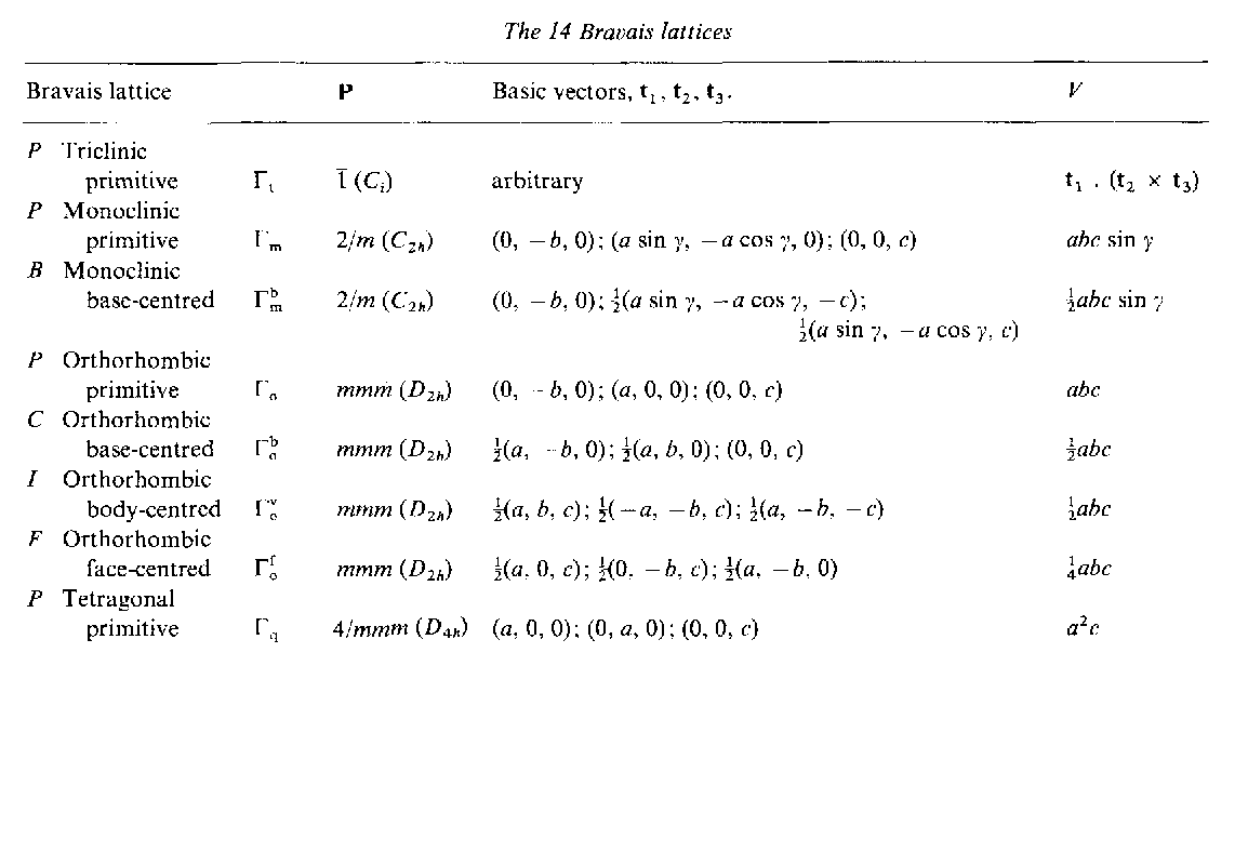
\includegraphics[width=0.92\textwidth]{c3_t31_p1.png}
\end{figure}
\begin{figure}[H]
\centering
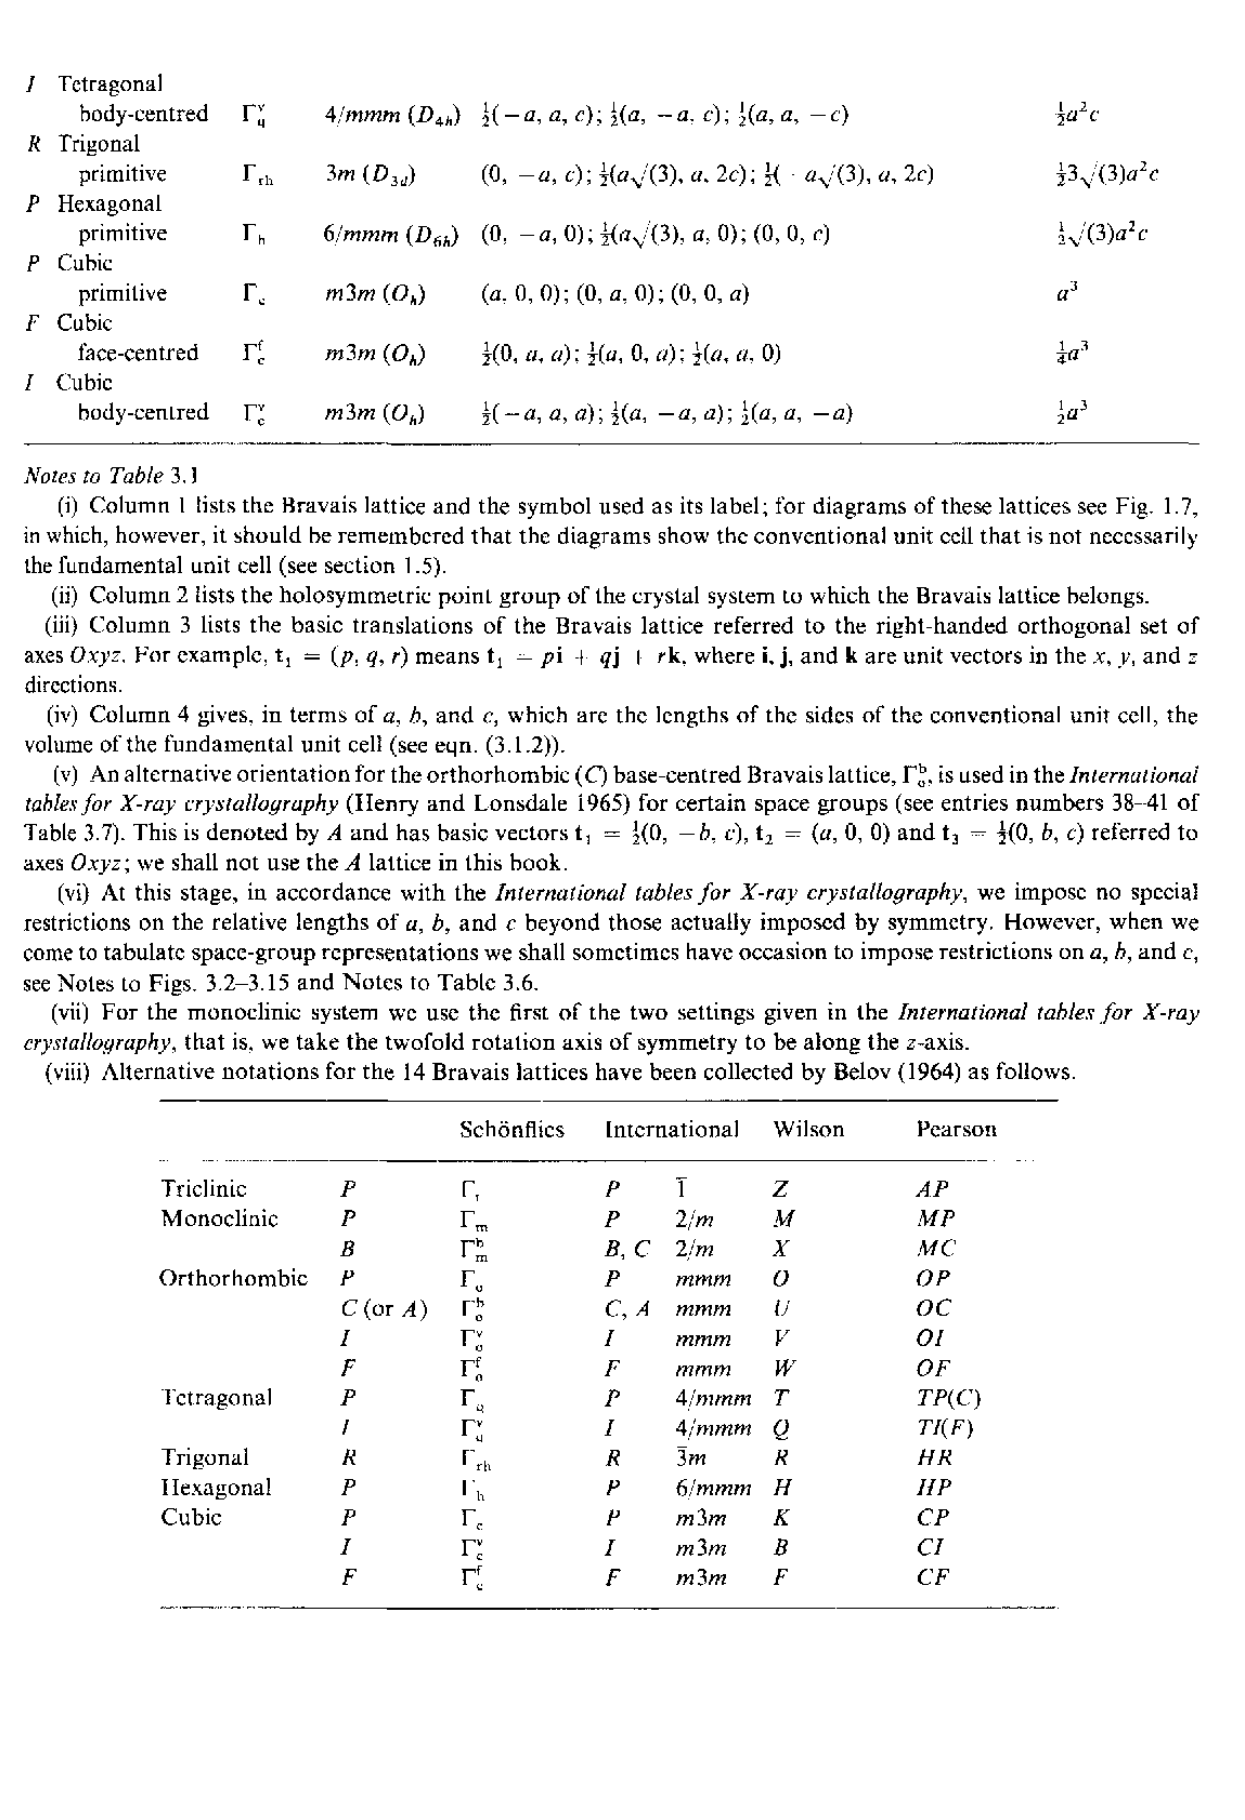
\includegraphics[width=0.92\textwidth]{c3_t31_p2.png}
\caption*{\textbf{表 3.1}\ 14 种布拉维格子：格子类型符号、Schönflies 记号 $\Gamma$、国际记号、基本平移（相对 $Oxyz$）与初基晶胞体积（原书扫描占位，含注 (i)--(viii)，见正文）。}
\end{figure}

七个晶系的对称元素见表 1.2。了解晶系的点群操作对格子平移的作用是有益的，这些作用列于表 3.2。

% 3.2 倒格子和布里渊区
\section{倒格子和布里渊区}

若布拉维格子的基本平移矢量为 $\mathbf{t}_{1}$、$\mathbf{t}_{2}$、$\mathbf{t}_{3}$，则可以定义一组倒格子（reciprocal lattice）矢量 $\mathbf{g}_{1}$、$\mathbf{g}_{2}$、$\mathbf{g}_{3}$，满足
\begin{equation*}
\mathbf{g}_{i} \cdot \mathbf{t}_{j} = 2\pi\delta_{ij} \qquad (i, j = 1, 2, 3).
\tag{3.2.1}
\end{equation*}
这样定义的倒格子当然早已为 X 射线晶体学家所广泛使用。一些作者在式中定义 $\mathbf{g}_{i}$ 时不含因子 $2\pi$，因而在后面的理论中不得不使用“$2\pi$ 乘一个倒格子矢量”这种笨拙的说法。由式 (3.2.1)，$\mathbf{g}_{1}$、$\mathbf{g}_{2}$、$\mathbf{g}_{3}$ 可显式地写为
\begin{equation*}
\left\{
\begin{array}{l}
\mathbf{g}_{1} = \dfrac{2\pi(\mathbf{t}_{2} \times \mathbf{t}_{3})}{\mathbf{t}_{1} \cdot (\mathbf{t}_{2} \times \mathbf{t}_{3})}, \\[2ex]
\mathbf{g}_{2} = \dfrac{2\pi(\mathbf{t}_{3} \times \mathbf{t}_{1})}{\mathbf{t}_{2} \cdot (\mathbf{t}_{3} \times \mathbf{t}_{1})}, \\[2ex]
\mathbf{g}_{3} = \dfrac{2\pi(\mathbf{t}_{1} \times \mathbf{t}_{2})}{\mathbf{t}_{3} \cdot (\mathbf{t}_{1} \times \mathbf{t}_{2})}.
\end{array}
\right.
\tag{3.2.2}
\end{equation*}
若 $\mathbf{t}_{1}$、$\mathbf{t}_{2}$、$\mathbf{t}_{3}$ 是某一布拉维格子的基本矢量，则 $\mathbf{g}_{1}$、$\mathbf{g}_{2}$、$\mathbf{g}_{3}$ 通常是同一布拉维格子（在倒空间中）的基本矢量。但有四种情形，$\mathbf{g}_{1}$、$\mathbf{g}_{2}$、$\mathbf{g}_{3}$ 是同一晶系中另一种布拉维格子的基本矢量。例如，考虑面心立方格子，由表 3.1 其基本矢量为
\begin{equation*}
\left\{
\begin{array}{l}
\mathbf{t}_{1} = \frac{1}{2}a(0, 1, 1), \\
\mathbf{t}_{2} = \frac{1}{2}a(1, 0, 1), \\
\mathbf{t}_{3} = \frac{1}{2}a(1, 1, 0).
\end{array}
\right.
\tag{3.2.3}
\end{equation*}
把它们代入式 (3.2.2)，得到
\begin{equation*}
\left\{
\begin{array}{l}
\mathbf{g}_{1} = \frac{2\pi}{a}(-1, 1, 1), \\
\mathbf{g}_{2} = \frac{2\pi}{a}(1, -1, 1), \\
\mathbf{g}_{3} = \frac{2\pi}{a}(1, 1, -1),
\end{array}
\right.
\tag{3.2.4}
\end{equation*}
对照表 3.1 即可看出，这些矢量定义的是一个体心立方格子。因此，立方面心格子的倒格子是立方体心格子，反之亦然；正交面心格子的倒格子同样是正交体心格子，反之亦然。四方体心格子的倒格子是它自身，因为四方面心格子同时也是轴比不同的四方体心格子。与正空间中的布拉维格子一样，我们可以把倒格子任一点的位矢 $\mathbf{g}$ 用 $\mathbf{g}_{1}$、$\mathbf{g}_{2}$、$\mathbf{g}_{3}$ 表示；仿照式 (1.5.1)，
\begin{equation*}
\mathbf{g} = n_{1}\mathbf{g}_{1} + n_{2}\mathbf{g}_{2} + n_{3}\mathbf{g}_{3}
\tag{3.2.5}
\end{equation*}
其中 $n_{1}$、$n_{2}$、$n_{3}$ 为整数。

正空间坐标我们用 $x$、$y$、$z$，倒空间坐标用 $k_{x}$、$k_{y}$、$k_{z}$，因为倒空间中的一般矢量习惯上记作 $\mathbf{k}$。应当注意，如果把倒格子叠加在正格子上作图，那么 $\mathbf{g}_{1}$ 垂直于 $\mathbf{t}_{2}$ 和 $\mathbf{t}_{3}$，并不一定沿 $\mathbf{t}_{1}$ 的方向。在空间群的表示理论中究竟为什么要引入倒空间，到 3.4 节讨论平移群的表示理论时就会明白了。

表 3.3 列出 14 种布拉维格子的倒格子矢量。倒格子基矢 $\mathbf{g}_{1}$、$\mathbf{g}_{2}$、$\mathbf{g}_{3}$ 在所属晶系点群操作 $R$ 下的变换，既可以从倒空间中的图看出，也可以解析地计算：对式 (3.2.2) 两边施加 $R$ 即可，结果列于表 3.4。任一倒格子矢量 $\mathbf{g}$ 在 $R$ 下的变换，则可对式 (3.2.5) 两边施加 $R$ 并利用表 3.4 求出。

\begin{figure}[H]
\centering
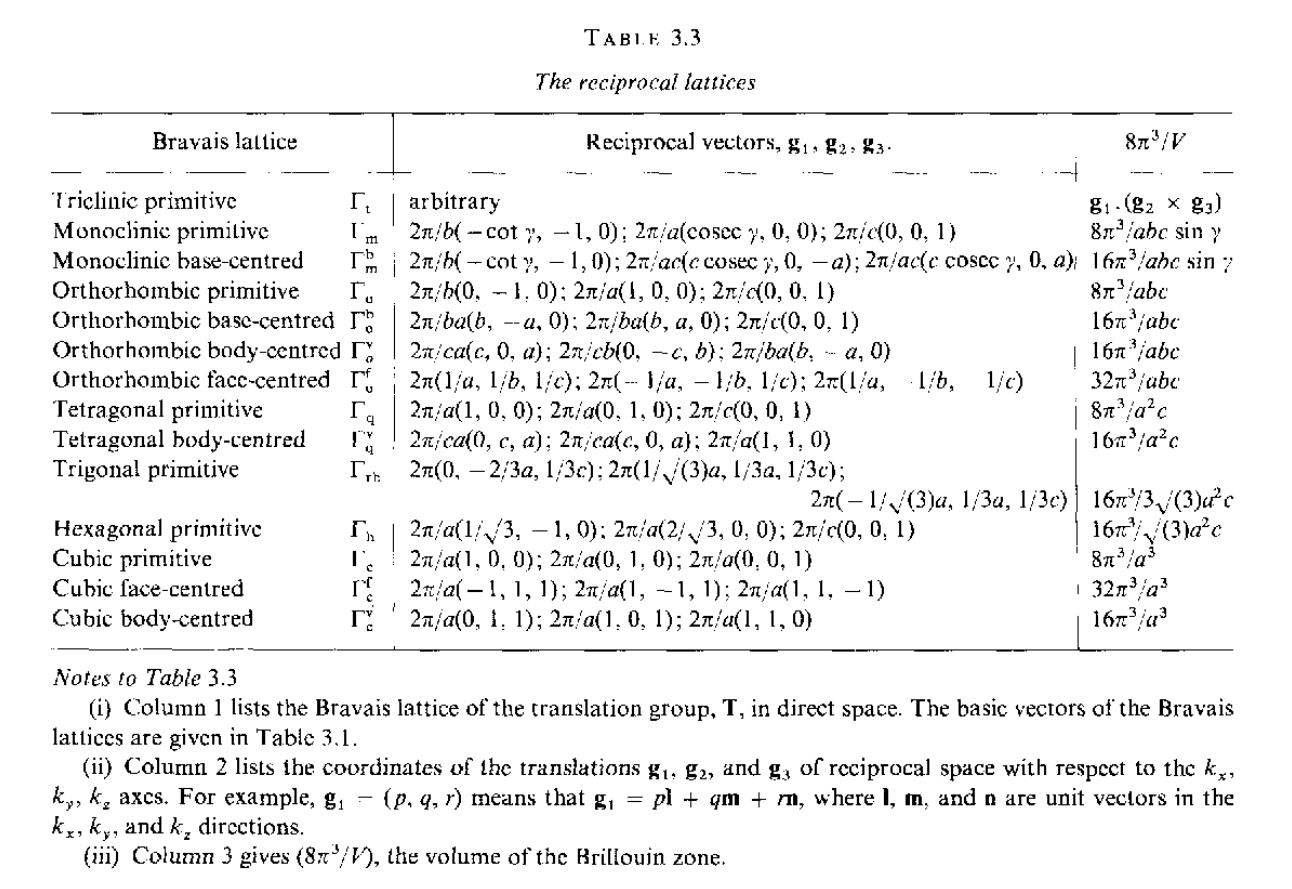
\includegraphics[width=0.92\textwidth]{c3_t33.png}
\caption*{\textbf{表 3.3}\ 倒格子（原书扫描占位）。左起各列：布拉维格子、$\Gamma$ 记号、倒格子矢量 $\mathbf{g}_{1}, \mathbf{g}_{2}, \mathbf{g}_{3}$、$8\pi^{3}/V$。注：}
\end{figure}
\noindent（i）第 1 列列出正空间平移群 $\mathbf{T}$ 的布拉维格子。各布拉维格子的基本矢量见表 3.1。

\noindent（ii）第 2 列列出倒空间平移 $\mathbf{g}_{1}$、$\mathbf{g}_{2}$、$\mathbf{g}_{3}$ 相对于 $k_{x}$、$k_{y}$、$k_{z}$ 轴的坐标。例如 $\mathbf{g}_{1} = (p, q, r)$ 表示 $\mathbf{g}_{1} = p\mathbf{l} + q\mathbf{m} + r\mathbf{n}$，其中 $\mathbf{l}$、$\mathbf{m}$、$\mathbf{n}$ 是 $k_{x}$、$k_{y}$、$k_{z}$ 方向的单位矢量。

\noindent（iii）第 3 列给出 $(8\pi^{3}/V)$，即布里渊区的体积。

\begin{figure}[H]
\centering
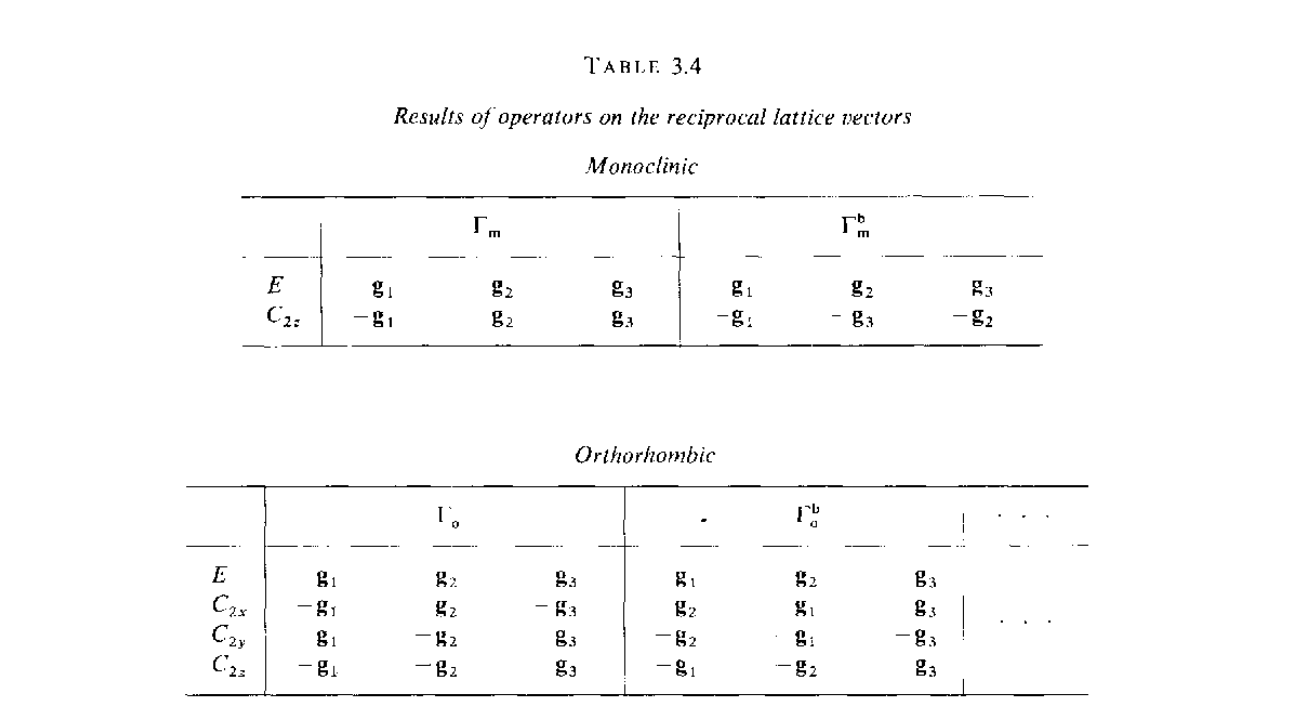
\includegraphics[width=0.78\textwidth]{c3_t34_p1.png}
\caption*{\textbf{表 3.4}\ 算符作用在倒格子矢量上的结果（第一部分：单斜、正交；原书扫描占位）。}
\end{figure}
\begin{figure}[H]
\centering
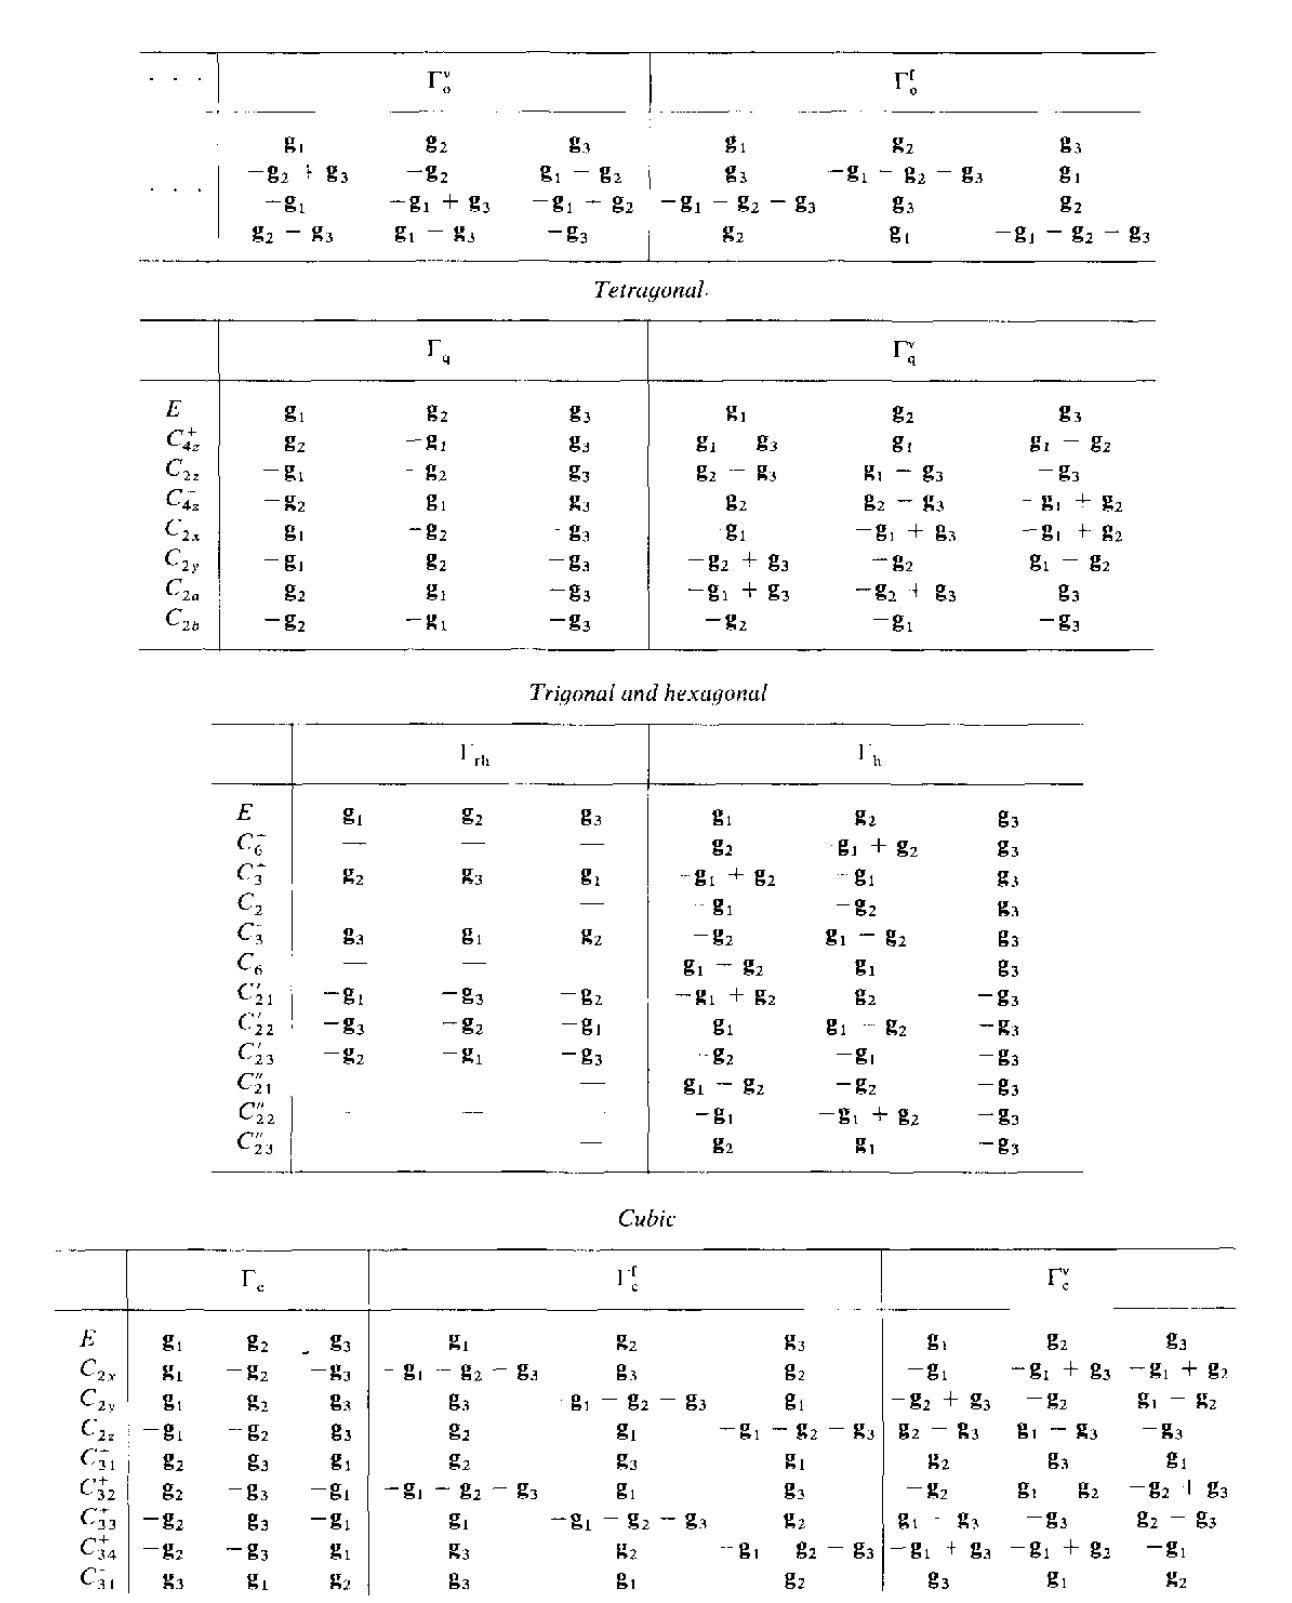
\includegraphics[width=0.86\textwidth]{c3_t34_p2.png}
\caption*{\textbf{表 3.4}（第二部分：正交续、四方、三角与六角、立方；原书扫描占位）。}
\end{figure}
\begin{figure}[H]
\centering
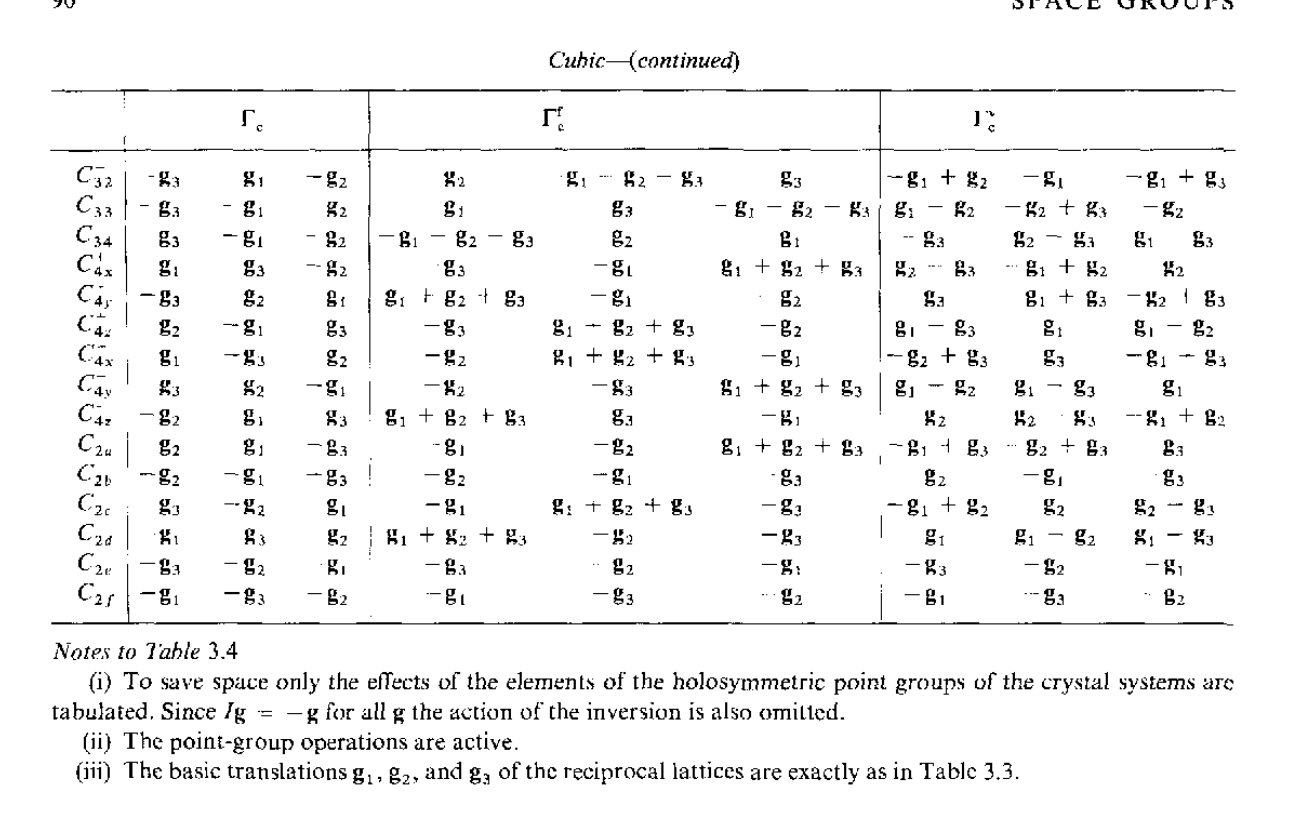
\includegraphics[width=0.88\textwidth]{c3_t34_p3.png}
\caption*{\textbf{表 3.4}（第三部分：立方续；原书扫描占位）。注：}
\end{figure}
\noindent（i）为节省篇幅，表中只列出各晶系全对称点群（holosymmetric point group）诸元素的作用。由于 $I\mathbf{g} = -\mathbf{g}$ 对一切 $\mathbf{g}$ 成立，反演的作用也一并略去。

\noindent（ii）点群操作是主动的（active）。

\noindent（iii）倒格子的基本平移 $\mathbf{g}_{1}$、$\mathbf{g}_{2}$、$\mathbf{g}_{3}$ 与表 3.3 中的完全一致。

接下来我们讨论布里渊区（Brillouin 1930\textit{a}--\textit{c}, 1931, 1953）。\textit{第一布里渊区}（first Brillouin zone）本质上是晶体倒格子的一个晶胞；这是布里渊区要发挥任何有用作用的必要条件。惯常选取的特定晶胞是倒格子的 Wigner--Seitz 晶胞（见 1.5 节）（Jones 1960, Slater 1965\textit{b}）。这时布里渊区定义如下：

\noindent\textbf{定义 3.2.1}\quad 以倒格点之一为原点的全部 $\mathbf{k}$ 矢量的集合，若具有性质：从其中任一矢量出发，加上倒格子的平移矢量，不能到达更短长度的矢量，则这个集合构成所谓\textit{第一布里渊区}。

实际上，对三斜和单斜空间群我们将不使用这个定义（见下面的定义 3.2.2）。

按这个定义构造第一布里渊区时，我们选定某个倒格点为原点，作出由它连向其余倒格点的矢量 $\mathbf{g}$。若画出这些倒格子矢量 $\mathbf{g}$ 的垂直平分面，那么第一布里渊区就是围绕原点、由这些平面围成的最小体积。$\mathbf{g}$ 的垂直平分面的方程为
\begin{equation*}
\mathbf{k} \cdot \mathbf{g} = \tfrac{1}{2}|\mathbf{g}|^{2}.
\tag{3.2.6}
\end{equation*}
于是第一布里渊区的每一个面都由一个倒格子矢量 $\mathbf{g}$ 表征，并且当然就是 $\mathbf{g}$ 的垂直平分面。之所以在倒空间选取 Wigner--Seitz 晶胞而不是别的晶胞，是因为这个晶胞展示出倒格子的点群对称性（例如见 Delaunay (1932)）。然而，对属于低对称晶系的晶体，用式 (3.2.6) 作图构造布里渊区极其繁琐。

另一种值得在此一并考虑的晶胞是初基晶胞（见 1.5 节），即以 $\mathbf{k} = \mathbf{0}$ 为中心、棱与倒格子基本矢量 $\mathbf{g}_{1}$、$\mathbf{g}_{2}$、$\mathbf{g}_{3}$ 平行且等长的平行六面体。第一布里渊区的体积便由
\begin{equation*}
\mathbf{g}_{1} \cdot (\mathbf{g}_{2} \times \mathbf{g}_{3}) = \frac{8\pi^{3}}{V}
\tag{3.2.7}
\end{equation*}
给出，其中 $V$ 是相应正格子初基晶胞的体积；每种倒格子的 $\mathbf{g}_{1} \cdot (\mathbf{g}_{2} \times \mathbf{g}_{3})$ 值见表 3.3。对某些倒格子（正交 $P$、四方 $P$ 和立方 $P$ 空间群的倒格子），用倒空间初基晶胞定义的布里渊区与用 Wigner--Seitz 晶胞定义的惯用布里渊区完全相同。对另一些倒格子（正交 $I$、四方 $I$、六角 $P$、立方 $F$ 和立方 $I$ 空间群的倒格子），初基晶胞不能在与正空间格子相同的取向上展示布拉维格子的点群对称性，此时初基晶胞便不能用来定义布里渊区，见表 3.5 第 2 列。这八种布拉维格子几乎涵盖了实际研究过布里渊区的全部晶体，因此人们通常把选取倒空间的 Wigner--Seitz 晶胞当作第一布里渊区定义的一个必要部分，这并不奇怪。然而，对其余六种布拉维格子（三斜 $P$、单斜 $P$、单斜 $B$、正交 $C$、正交 $F$ 和三方 $R$ 空间群的），可以直接看出倒格子的初基晶胞也以正确的取向具有晶体布拉维格子的点群对称性。不过，只要可能，最好让布里渊区的界面平行于晶体中的对称面。这意味着对正交 $C$ 与 $F$ 空间群，在定义布里渊区时宜保留 Wigner--Seitz 胞，见图 3.6 与图 3.8。至于三方 $R$ 格子，似乎也没有什么特别有力的理由要用倒空间的初基晶胞去取代惯用的布里渊区定义。但对剩下的三种格子（三斜 $P$、单斜 $P$ 和单斜 $B$ 空间群的），如前所述，无论要画出布里渊区的形状，还是画出之后要在头脑中想象它，式 (3.2.6) 在实际应用中都十分困难，其形状细节在很大程度上依赖于所论晶体晶胞参数的具体取值。对单斜晶体，一些作者（Koster 1957, Sushkevich 1966）对每种布拉维格子各画出一个特定例子，Luehrmann (1968) 对单斜 $B$ 格子给出了两个例子，而 Kovalev (1965) 的详表则完全没有布里渊区图。因此，对单斜或三斜晶体采用初基晶胞定义布里渊区有一个优点：其总体形状（即棱数和面数）不依赖于晶体晶胞的轴比和轴间角。

\begin{table}[H]
\centering
\caption*{\textbf{表 3.5}\ 第 2 列标出：由倒空间初基晶胞定义的布里渊区是否以正确取向具有晶体的点群对称性；第 3 列标出：满足前一条件、且倒空间的 Wigner--Seitz 胞与初基胞给出相同布里渊区形状的那些布拉维格子。}
\begin{tabular}{@{}lcccclccc@{}}
\toprule
布拉维格子 & 2 & 3 & \phantom{xxxx} & 布拉维格子 & 2 & 3 \\
\midrule
三斜 $P$   & $\checkmark$ & $\times$ & & 四方 $P$ & $\checkmark$ & $\checkmark$ \\
单斜 $P$   & $\checkmark$ & $\times$ & & 四方 $I$ & $\times$ & --- \\
单斜 $B$   & $\checkmark$ & $\times$ & & 三方 $R$ & $\checkmark$ & $\times$ \\
正交 $P$   & $\checkmark$ & $\checkmark$ & & 六角 $P$ & $\times$ & --- \\
正交 $C$   & $\checkmark$ & $\times$ & & 立方 $P$ & $\checkmark$ & $\checkmark$ \\
正交 $I$   & $\times$ & --- & & 立方 $F$ & $\times$ & --- \\
正交 $F$   & $\checkmark$ & $\times$ & & 立方 $I$ & $\times$ & --- \\
\bottomrule
\end{tabular}
\end{table}

因此我们建议：大多数晶体的布里渊区仍用倒空间的 Wigner--Seitz 胞来定义，但对单斜和三斜空间群，应当改用倒空间的初基晶胞（Bradley and Cracknell 1970）。在构造图 3.2--3.4 时我们遵循了这一做法。

\noindent\textbf{定义 3.2.2}\quad 对单斜或三斜晶体，第一布里渊区取为倒格子的初基晶胞，即以 $\mathbf{k} = \mathbf{0}$ 为中心、棱与倒格子基本矢量 $\mathbf{g}_{1}$、$\mathbf{g}_{2}$、$\mathbf{g}_{3}$ 平行且等长的平行六面体。

最后还应指出一点。有人认为式 (3.2.6) 与电子、声子或磁振子的能量 $E(\mathbf{k})$ 随 $\mathbf{k}$ 变化曲线中出现不连续有特殊关联。其实并非如此，因为无论在扩展区图式还是重复区图式中，$E(\mathbf{k})$ 在倒空间处处都是 $\mathbf{k}$ 的准连续函数（Koopmans 定理）。划定区界时出现的不连续，不过是不同的 $E(\mathbf{k})$ 曲线在此分开。当然，有时可以细心地选取区界，使得 $E(\mathbf{k})$ 在区界处呈现特殊的简并；然而这一性质来源于“布里渊区应当展示布拉维格子的正确点群对称性”这一要求——我们并没有放弃这个要求——而不是使用 Wigner--Seitz 胞和式 (3.2.6) 的结果。

用式 (3.2.6) 构造第一布里渊区时，倒格子矢量 $\mathbf{g}$ 是由原点连向它的第一近邻、可能还有第二或更远近邻的矢量。还可以利用式 (3.2.6) 的更多平面，在第一布里渊区之外围出一个满足下列三个条件的体积，从而定义第二布里渊区：(i) 第二布里渊区的体积等于第一布里渊区的体积；(ii) 对第一布里渊区中的每个 $\mathbf{k}$ 矢量 $\mathbf{k}_{1}$，在第二布里渊区中恰有一个 $\mathbf{k}$ 矢量 $\mathbf{k}_{2}$，使得
\begin{equation*}
\mathbf{k}_{2} - \mathbf{k}_{1} = \mathbf{g},
\tag{3.2.8}
\end{equation*}
其中 $\mathbf{g}$ 是一个倒格子矢量，但对所有 $\mathbf{k}_{1}$ 不必相同。于是，第二布里渊区中的每一点都在某种意义上（3.3 节将更严格地定义）等价于第一布里渊区中的某一点；(iii) 第二布里渊区中的 $\mathbf{k}$ 矢量必须取满足条件 (i) 与 (ii) 的最短者。类似地可以定义第三、第四以及更高阶的布里渊区。

在给任一给定晶体定义布里渊区时，务必小心使用描述晶体\textit{全部}平移对称性的布拉维格子，而不要用晶胞更大的其他格子（Barron and Fischer 1959）。一旦完整认定了布拉维格子，倒格子与布里渊区的结构便唯一确定；它们与晶胞内部原子的具体排布完全无关。如上定义的布里渊区具有如下性质：

\noindent(i) 晶体的布拉维格子每个初基晶胞在区中对应一个态（对电子，泡利不相容原理允许自旋为 $+\frac{1}{2}$ 和 $-\frac{1}{2}$ 的两个电子占据每个这样的态；对声子或磁振子，当然不存在这样的不相容原理）（见式 (3.4.5)）。

\noindent(ii) 晶体中粒子或准粒子的能量在每个区内部处处连续。

\noindent(iii) 更高阶区的各分区可以通过适当的倒格子矢量平移而搬入第一区，这样每个区的态便在第一区上构成一条连续能带；这称为\textit{约化区图式}（reduced zone scheme）。

\noindent(iv) 具有第一布里渊区形状的胞可以相互拼合，完全填满倒空间，即相邻胞之间不留空隙。这称为\textit{重复区图式}（repeated zone scheme），常常有用。

在倒空间中定义区的另一种方法（Jones 1934\textit{a}）主张：只有那些对应的 Bragg 反射具有非零结构因子（structure factor）的平面才是真正的区界。这些 \textit{Jones 区}（Jones zones）在许多标准教科书中已有讨论（例如 Jones (1960), Kittel (1956), Mott and Jones (1936), Wilson (1953)），但如今似乎已很少使用。

\begin{figure}[H]
\centering
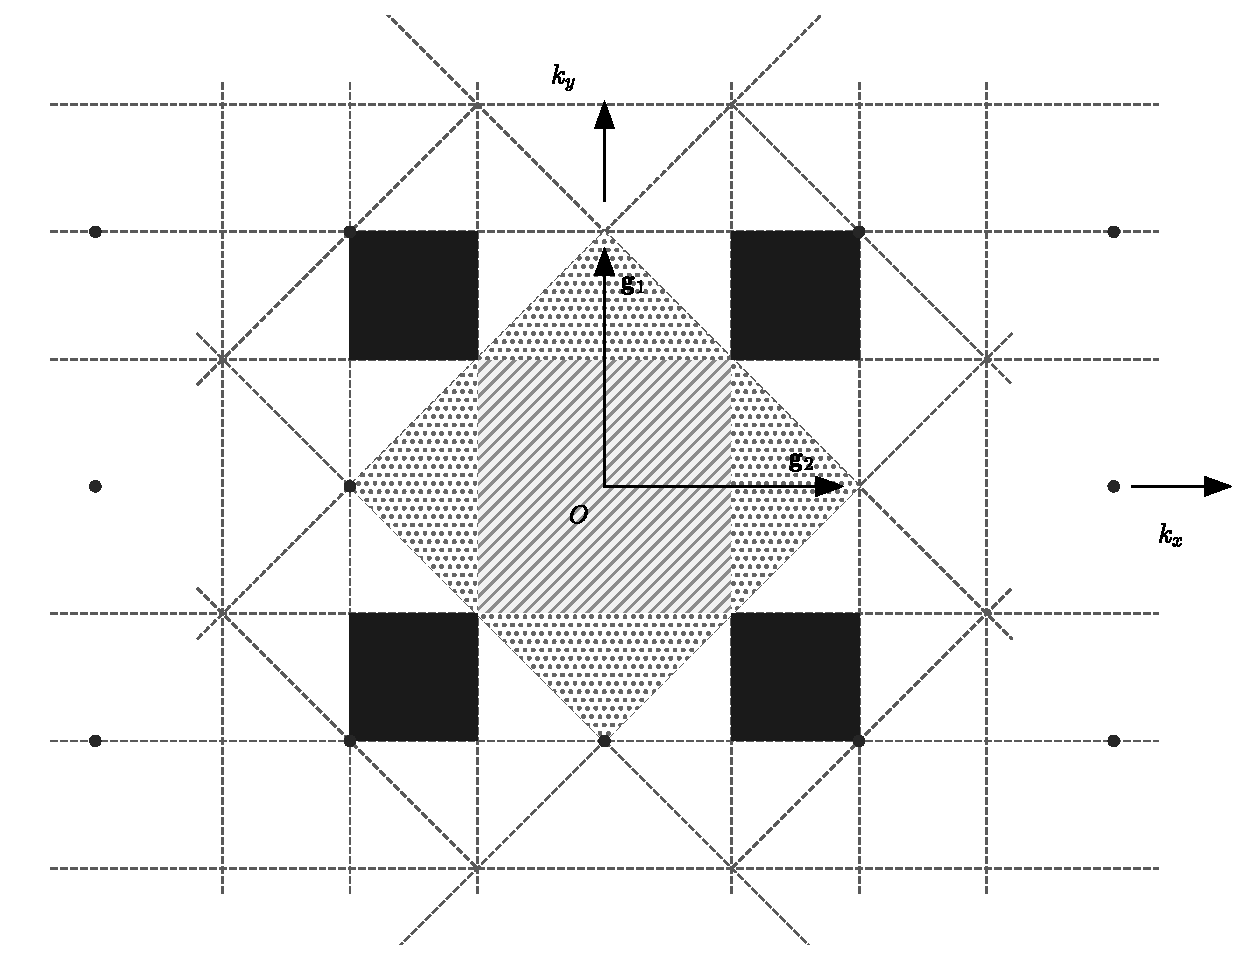
\includegraphics[width=0.92\textwidth]{fig3_1.pdf}
\caption{二维正方布拉维格子 $p$ 的前三个布里渊区（依原书重绘）。}
\end{figure}

我们用一个二维的例子来说明第一、第二及更高阶布里渊区的概念。二维正方布拉维格子 $p$ 的基本矢量可取为
\begin{equation*}
\left\{
\begin{array}{l}
\mathbf{t}_{1} = a\mathbf{i} \\
\mathbf{t}_{2} = a\mathbf{j}
\end{array}
\right.
\tag{3.2.9}
\end{equation*}
其中 $\mathbf{i}$、$\mathbf{j}$ 是 $x$、$y$ 方向的单位矢量。满足式 (3.2.1) 的倒格子矢量 $\mathbf{g}_{1}$、$\mathbf{g}_{2}$ 于是为
\begin{equation*}
\left\{
\begin{array}{l}
\mathbf{g}_{1} = \frac{2\pi}{a}\mathbf{j} \\
\mathbf{g}_{2} = \frac{2\pi}{a}\mathbf{i}.
\end{array}
\right.
\tag{3.2.10}
\end{equation*}
第一布里渊区是 $k_{x} = \pm\frac{1}{2}|\mathbf{g}_{2}| = \pm\pi/a$ 与 $k_{y} = \pm\frac{1}{2}|\mathbf{g}_{1}| = \pm\pi/a$ 之间的区域，也就是说，代入式 (3.2.6) 的矢量 $\mathbf{g}$ 是 $+\mathbf{g}_{1}$、$-\mathbf{g}_{1}$、$+\mathbf{g}_{2}$ 和 $-\mathbf{g}_{2}$。于是第一布里渊区就是图 3.1 中画有斜线阴影的正方形。对第二布里渊区，代入式 (3.2.6) 的矢量是 $\mathbf{g}_{1}+\mathbf{g}_{2}$、$-\mathbf{g}_{1}+\mathbf{g}_{2}$、$\mathbf{g}_{1}-\mathbf{g}_{2}$ 和 $-\mathbf{g}_{1}-\mathbf{g}_{2}$，第二布里渊区因而是图 3.1 中标有点点的区域。事实上我们只使用第一布里渊区，所以从现在起省略“第一”这个定语。

按照 Bouckaert, Smoluchowski, and Wigner (1936) 的说法，这些区的存在几乎同时被多位作者注意到（Bloch 1928, Morse 1930, Peierls 1930, Strutt 1928\textit{a},\textit{b}），而 Brillouin（1930\textit{a}--\textit{c}, 1931）指出了它们与 X 射线反射的联系。关于布里渊区已有一本教科书（Jones 1960）。

% 3.3 对称点和对称线的分类
\section{对称点和对称线的分类}

对某些格子，布里渊区的形状是唯一的；而对另一些格子，则有两种或更多种可能的形状，取决于基本平移的相对大小和它们之间的夹角。正空间 14 种布拉维格子的各种布里渊区示于图 3.2--3.15。

若 $(\mathbf{k}_{1} - \mathbf{k}_{2}) = a_{1}\mathbf{g}_{1} + a_{2}\mathbf{g}_{2} + a_{3}\mathbf{g}_{3}$，其中 $a_{1}$、$a_{2}$、$a_{3}$ 为整数，则称矢量 $\mathbf{k}_{1}$ 与 $\mathbf{k}_{2}$ \textit{等价}。由于其构造方式，布里渊区内部任何两点都不等价；但区面上的一个点可以与区面上一个或多个其他点等价。例如，一个面的中点总与对面中点等价，因为相对的面总相差一个倒格子矢量。

给定一个布里渊区和区内一点 $\mathbf{k}$，相应晶系的全对称点群 $\mathbf{P}$ 中存在某些元素，它们把 $\mathbf{k}$ 变换到它自身或某个与它等价的 $\mathbf{k}$ 矢量。这些元素构成 $\mathbf{P}$ 的一个子群，记作 $\mathbf{P}(\mathbf{k})$，称为 $\mathbf{k}$ 的\textit{对称群}（symmetry group）。现在可以给出对称点、对称线和对称面的定义。

\noindent\textbf{定义 3.3.1}\quad 若存在 $\mathbf{k}$ 的一个邻域 $N$，使得在 $N$ 内除 $\mathbf{k}$ 以外没有任何点具有对称群 $\mathbf{P}(\mathbf{k})$，则称 $\mathbf{k}$ 是一个\textit{对称点}（point of symmetry）。

也就是说，若 $\mathbf{k}' \in N$ 且 $\mathbf{k}' \neq \mathbf{k}$，则 $\mathbf{P}(\mathbf{k}')$ 总是 $\mathbf{P}(\mathbf{k})$ 的真子群。我们可以粗略地说，点 $\mathbf{k}$ 比它周围所有的点对称性都高。

\noindent\textbf{定义 3.3.2}\quad 若在 $\mathbf{k}$ 的任一充分小邻域 $N$ 中，总有一条线（一个平面）穿过 $\mathbf{k}$，其上所有点都与 $\mathbf{k}$ 具有相同的对称群，则称 $\mathbf{k}$ 是一条\textit{对称线}（line of symmetry）（一个\textit{对称面}（plane of symmetry））。

最后，若在 $\mathbf{k}$ 的任一充分小邻域 $N$ 中所有点都具有相同的对称群，则称 $\mathbf{k}$ 为\textit{一般点}（general point）。对一般点，$\mathbf{P}(\mathbf{k})$ 仅由恒等元构成。对对称面，$\mathbf{P}(\mathbf{k})$ 由恒等元和一个镜面反射构成，只有两个元素。

\noindent\textbf{定义 3.3.3}\quad 对每个布里渊区存在一个\textit{基本域}（basic domain）$\Omega$，使得 $(\Sigma_{R} R\Omega)$ 等于整个布里渊区，其中 $R$ 取遍相关晶系全对称点群 $\mathbf{P}$ 的元素。

因此
\begin{equation*}
\Omega = \frac{8\pi^{3}}{V|\mathbf{P}|}
\tag{3.3.1}
\end{equation*}
其中 $|\mathbf{P}|$ 是 $\mathbf{P}$ 的阶。

对称点的求法是：对交于该点的各个平面使用式 (3.2.6)，算出每个面心和每个顶点的坐标，然后看在相关全对称点群 $\mathbf{P}$ 的操作下（见表 3.1），这些点是否具有邻域内其他点都不具备的额外对称操作。这里所说的对称操作是指把矢量 $\mathbf{k}$ 变换为 $\mathbf{k}$ 本身或与 $\mathbf{k}$ 相差一个倒格子矢量的矢量 $\mathbf{k}'$ 的操作。类似的手续也可用于辨认对称线。所有布拉维格子布里渊区的各种对称点和对称线都已在图 3.2--3.15 的图中标出。我们在图 3.2--3.15 中用于对称点和对称线的字母几乎都是标准的，并尽可能与前人（Bouckaert, Smoluchowski, and Wigner 1936, Herring 1942, Koster 1955, Luehrmann 1968, Meijer and Bauer 1962, Miller and Love 1967）的记号一致。

% ---- 图 3.2 -- 3.6（MinerU 提取图；题注坐标已逐条对照扫描页核对，见进度文件）----
\begin{figure}[H]
\centering
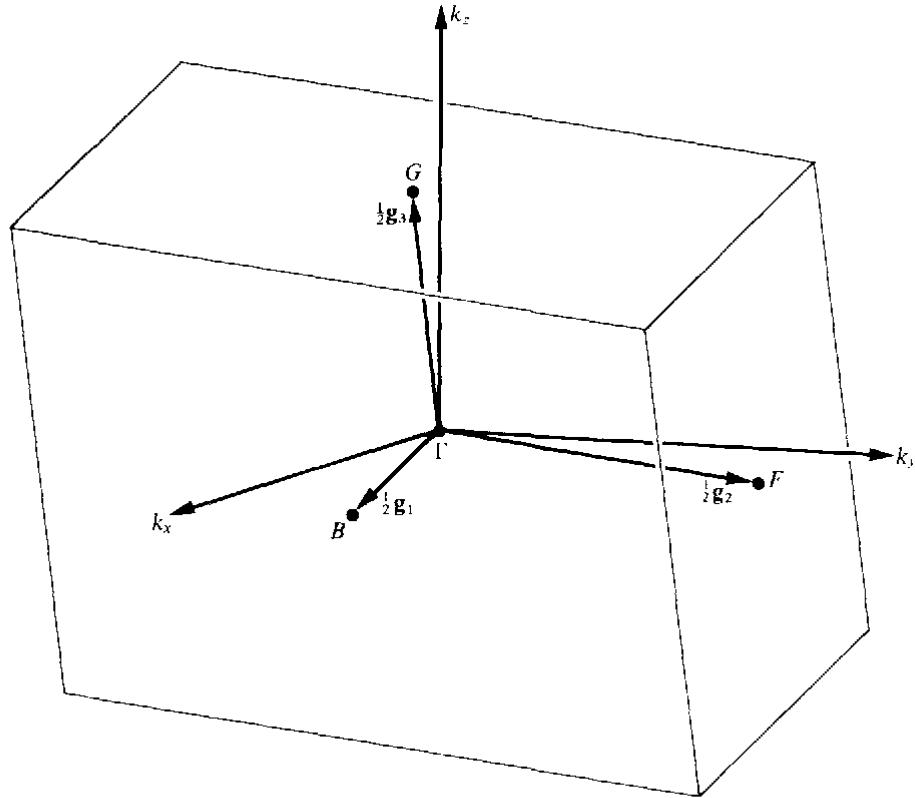
\includegraphics[width=0.60\textwidth]{fig3_2_mu.jpg}
\caption*{\textbf{图 3.2}\ $\Gamma_{t}$（三斜 $P$）的布里渊区。$\Gamma=(000)$；$B=(\frac{1}{2}00)$；$F=(0\frac{1}{2}0)$；$G=(00\frac{1}{2})$。}
\end{figure}
\begin{figure}[H]
\centering
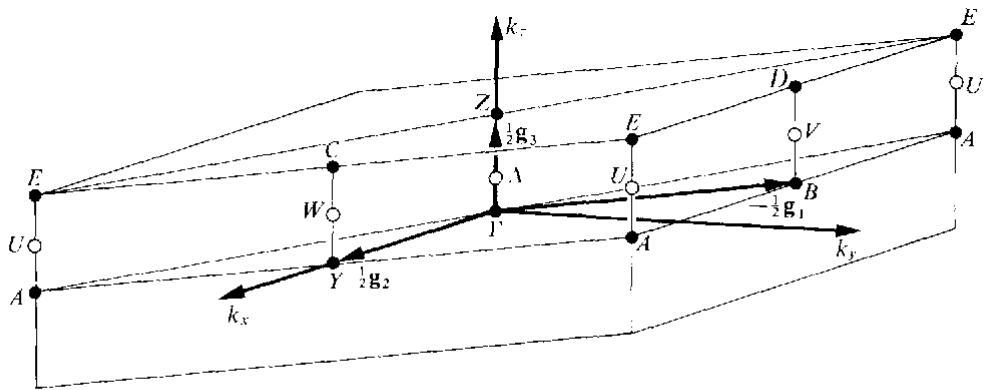
\includegraphics[width=0.64\textwidth]{fig3_3_mu.jpg}
\caption*{\textbf{图 3.3}\ $\Gamma_{m}$（单斜 $P$）的布里渊区。$\Gamma=(000)$；$B=(\bar{\frac{1}{2}}00)$；$Y=(0\frac{1}{2}0)$；$Z=(00\frac{1}{2})$；$C=(0\frac{1}{2}\frac{1}{2})$；$D=(\bar{\frac{1}{2}}0\frac{1}{2})$；$A=(\bar{\frac{1}{2}}\bar{\frac{1}{2}}0)$、$(\bar{\frac{1}{2}}\frac{1}{2}0)$ 或 $(\frac{1}{2}\bar{\frac{1}{2}}0)$；$E=(\bar{\frac{1}{2}}\bar{\frac{1}{2}}\frac{1}{2})$、$(\bar{\frac{1}{2}}\frac{1}{2}\frac{1}{2})$ 或 $(\frac{1}{2}\bar{\frac{1}{2}}\frac{1}{2})$。}
\end{figure}
\begin{figure}[H]
\centering
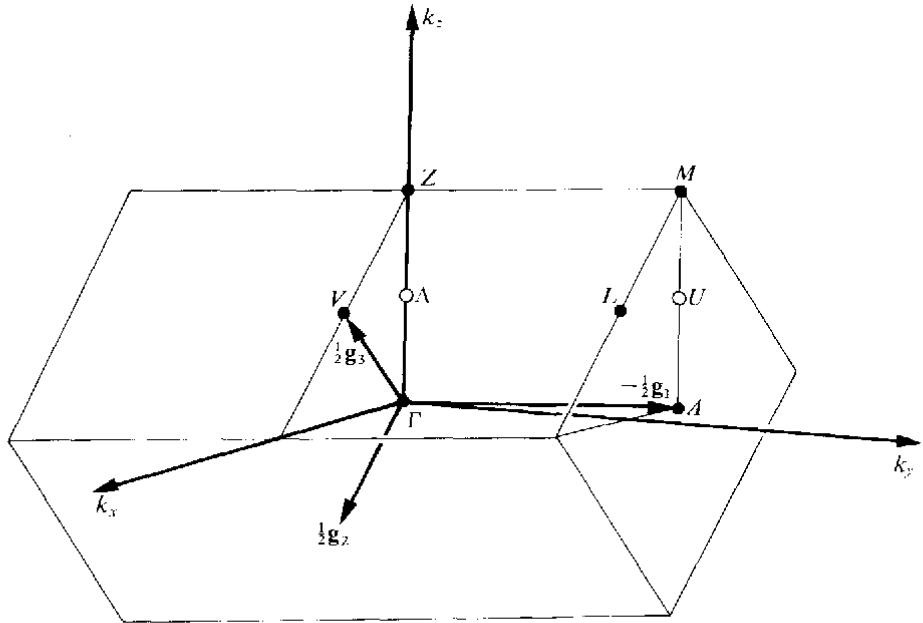
\includegraphics[width=0.64\textwidth]{fig3_4_mu.jpg}
\caption*{\textbf{图 3.4}\ $\Gamma_{m}^{b}$（单斜 $B$）的布里渊区。$\Gamma=(000)$；$A=(\frac{1}{2}00)$；$Z=(0\frac{1}{2}\frac{1}{2})$；$M=(\frac{1}{2}\frac{1}{2}\frac{1}{2})$；$L=(\frac{1}{2}0\frac{1}{2})$；$V=(00\frac{1}{2})$。}
\end{figure}
\begin{figure}[H]
\centering
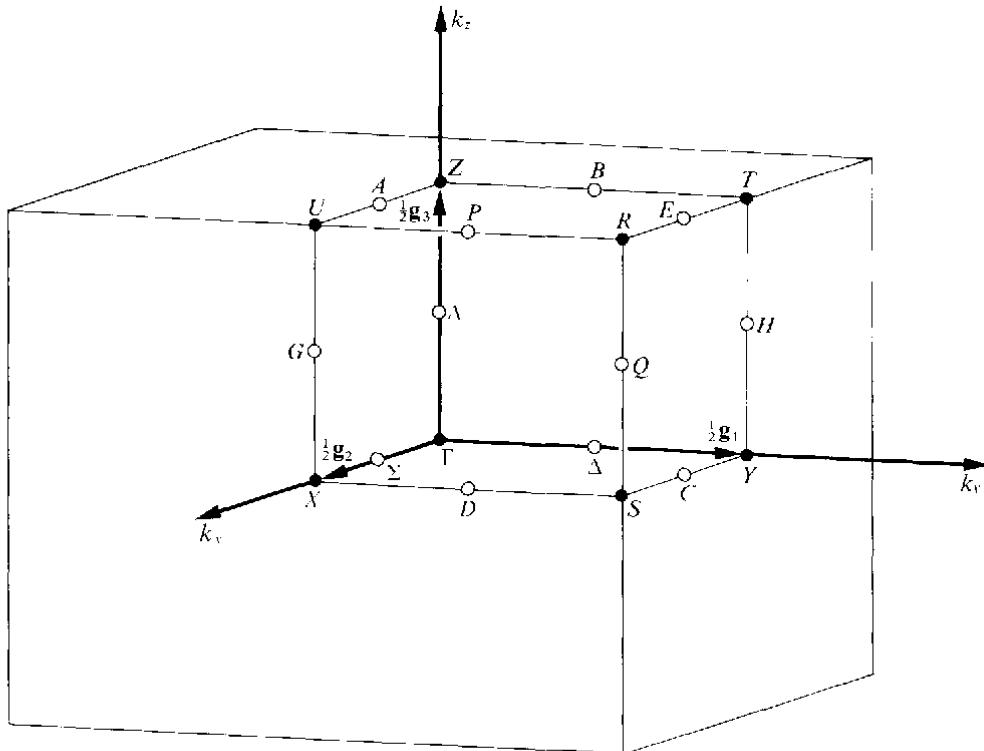
\includegraphics[width=0.64\textwidth]{fig3_5_mu.jpg}
\caption*{\textbf{图 3.5}\ $\Gamma_{o}$（正交 $P$）的布里渊区。$\Gamma=(000)$；$Y=(\frac{1}{2}00)$；$X=(0\frac{1}{2}0)$；$Z=(00\frac{1}{2})$；$U=(0\frac{1}{2}\frac{1}{2})$；$T=(\frac{1}{2}0\frac{1}{2})$；$S=(\frac{1}{2}\frac{1}{2}0)$；$R=(\frac{1}{2}\frac{1}{2}\frac{1}{2})$。}
\end{figure}
\begin{figure}[H]
\centering
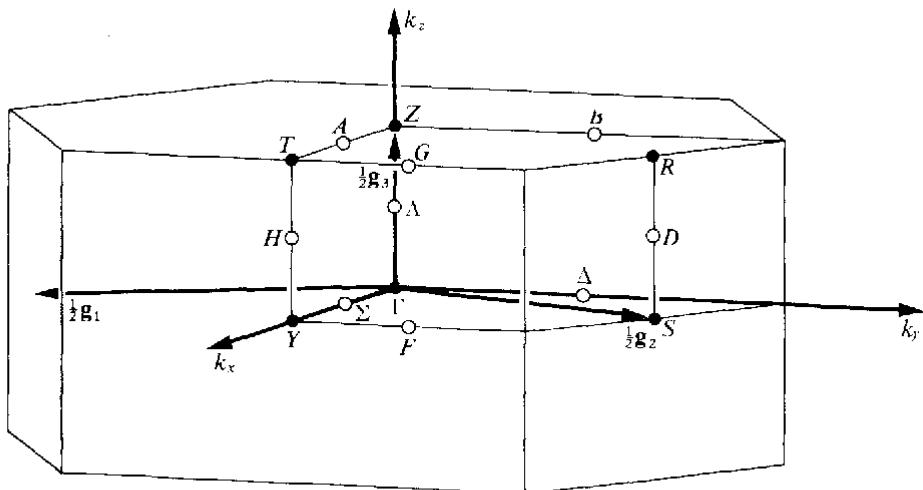
\includegraphics[width=0.58\textwidth]{fig3_6a_mu.jpg}\\[1ex]
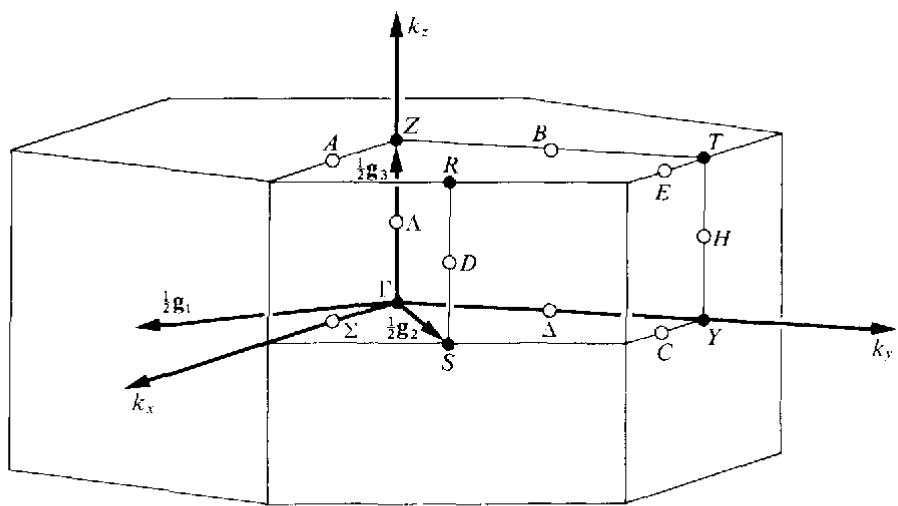
\includegraphics[width=0.58\textwidth]{fig3_6b_mu.jpg}
\caption*{\textbf{图 3.6}\ $\Gamma_{o}^{b}$（正交 $C$）的布里渊区：(a) $a>b$，$\Gamma=(000)$；$Y=(\frac{1}{2}\frac{1}{2}0)$；$Z=(00\frac{1}{2})$；$T=(\frac{1}{2}\frac{1}{2}\frac{1}{2})$；$S=(0\frac{1}{2}0)$；$R=(0\frac{1}{2}\frac{1}{2})$；(b) $b>a$，$\Gamma=(000)$；$Y=(\frac{1}{2}\frac{1}{2}0)$；$Z=(00\frac{1}{2})$；$T=(\frac{1}{2}\frac{1}{2}\frac{1}{2})$；$S=(0\frac{1}{2}0)$；$R=(0\frac{1}{2}\frac{1}{2})$。}
\end{figure}

在继续讲下面的图之前，先说明一下我们的做法。对三斜布拉维格子（图 3.2）和两种单斜布拉维格子（图 3.3 与图 3.4），我们按照定义 3.2.2 用倒空间的初基晶胞来定义布里渊区（见图注 (ii)）。其余格子的布里渊区用倒空间的 Wigner--Seitz 晶胞定义。

\begin{figure}[H]
\centering
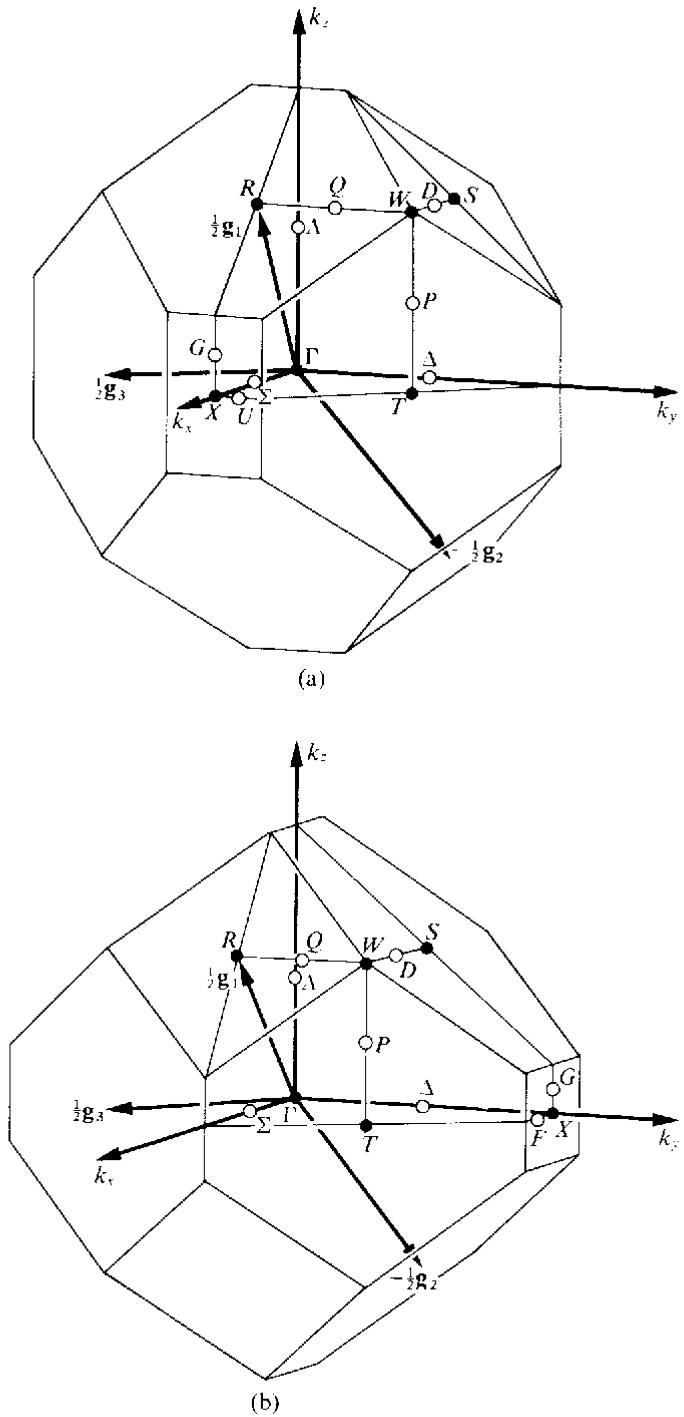
\includegraphics[width=0.62\textwidth]{fig3_7ab_mu.jpg}\\[1ex]
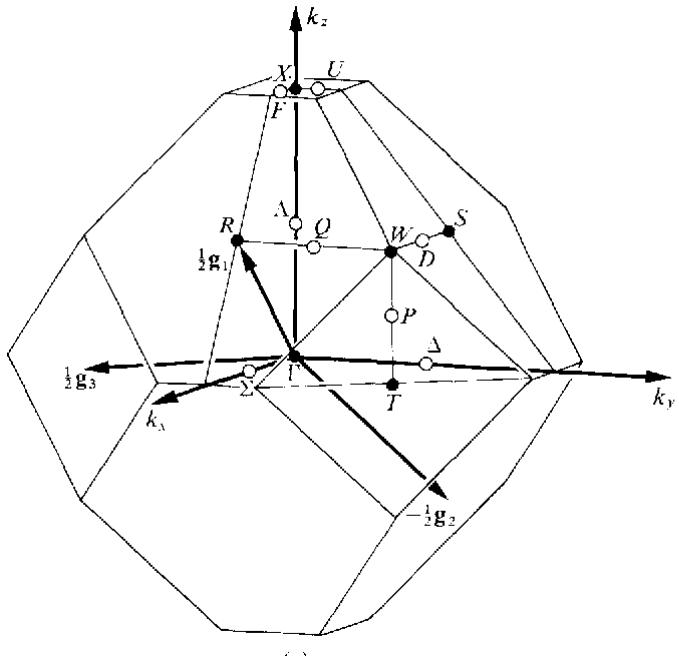
\includegraphics[width=0.62\textwidth]{fig3_7c_mu.jpg}
\caption*{\textbf{图 3.7}\ $\Gamma_{o}^{v}$（正交 $I$）的布里渊区：(a) $a>b>c$ 或 $a>c>b$，$\Gamma=(000)$；$X=(\frac{1}{2}\bar{\frac{1}{2}}\frac{1}{2})$；$R=(\bar{\frac{1}{2}}00)$；$S=(\frac{1}{2}0\bar{\frac{1}{2}})$；$T=(\frac{1}{2}\bar{\frac{1}{2}}0)$；$W=(\frac{3}{4}\bar{\frac{1}{2}}\frac{3}{4})$；(b) $b>a>c$ 或 $b>c>a$，$\Gamma=(000)$；$X=(\frac{1}{2}\frac{1}{2}\bar{\frac{1}{2}})$；$R=(\bar{\frac{1}{2}}00)$；$S=(\frac{1}{2}0\bar{\frac{1}{2}})$；$T=(\frac{1}{2}\bar{\frac{1}{2}}0)$；$W=(\frac{3}{4}\bar{\frac{1}{2}}\frac{3}{4})$；(c) $c>b>a$ 或 $c>a>b$，$\Gamma=(000)$；$X=(\frac{1}{2}\bar{\frac{1}{2}}\frac{1}{2})$；$R=(\bar{\frac{1}{2}}00)$；$S=(\frac{1}{2}0\bar{\frac{1}{2}})$；$T=(\frac{1}{2}\bar{\frac{1}{2}}0)$；$W=(\frac{3}{4}\bar{\frac{1}{2}}\frac{3}{4})$。}
\end{figure}
\begin{figure}[H]
\centering
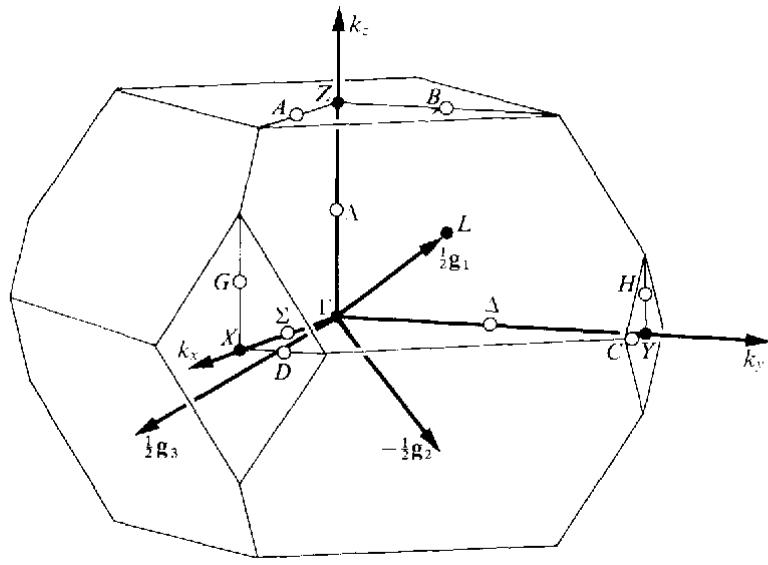
\includegraphics[width=0.60\textwidth]{fig3_8a_mu.jpg}\\[1ex]
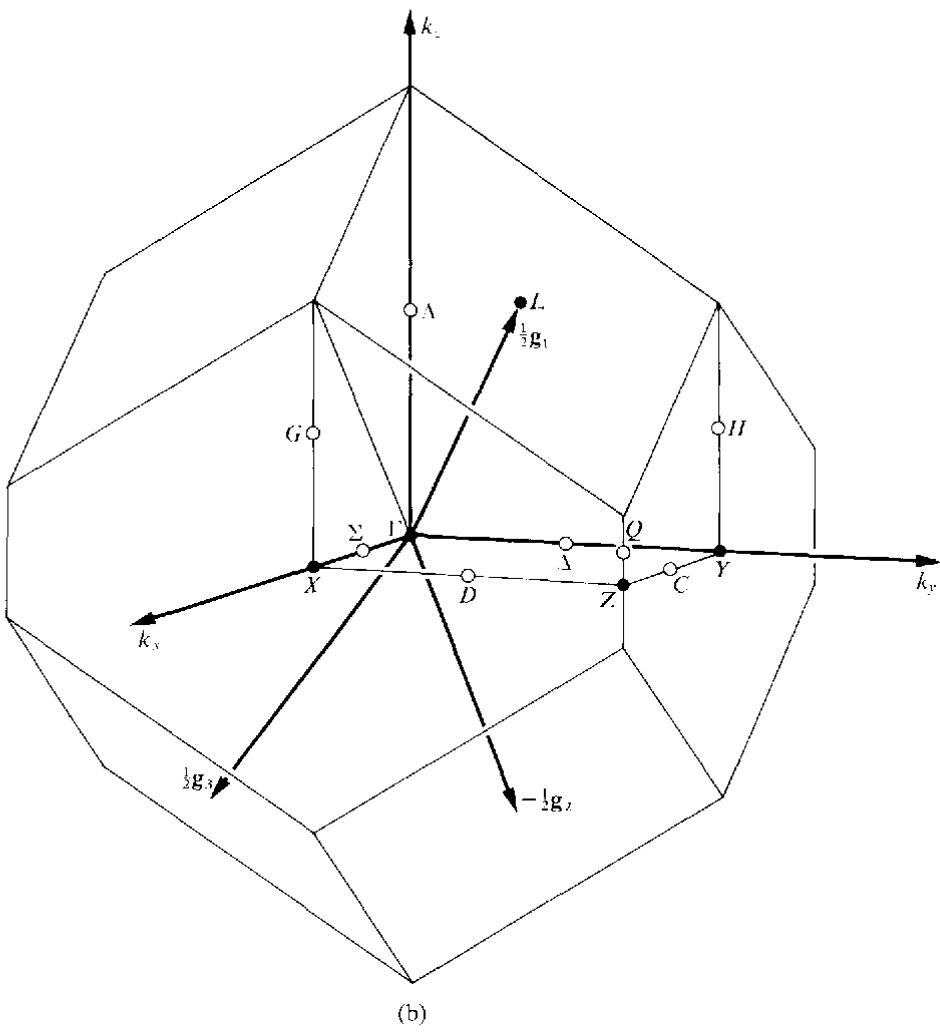
\includegraphics[width=0.60\textwidth]{fig3_8b_mu.jpg}\\[1ex]
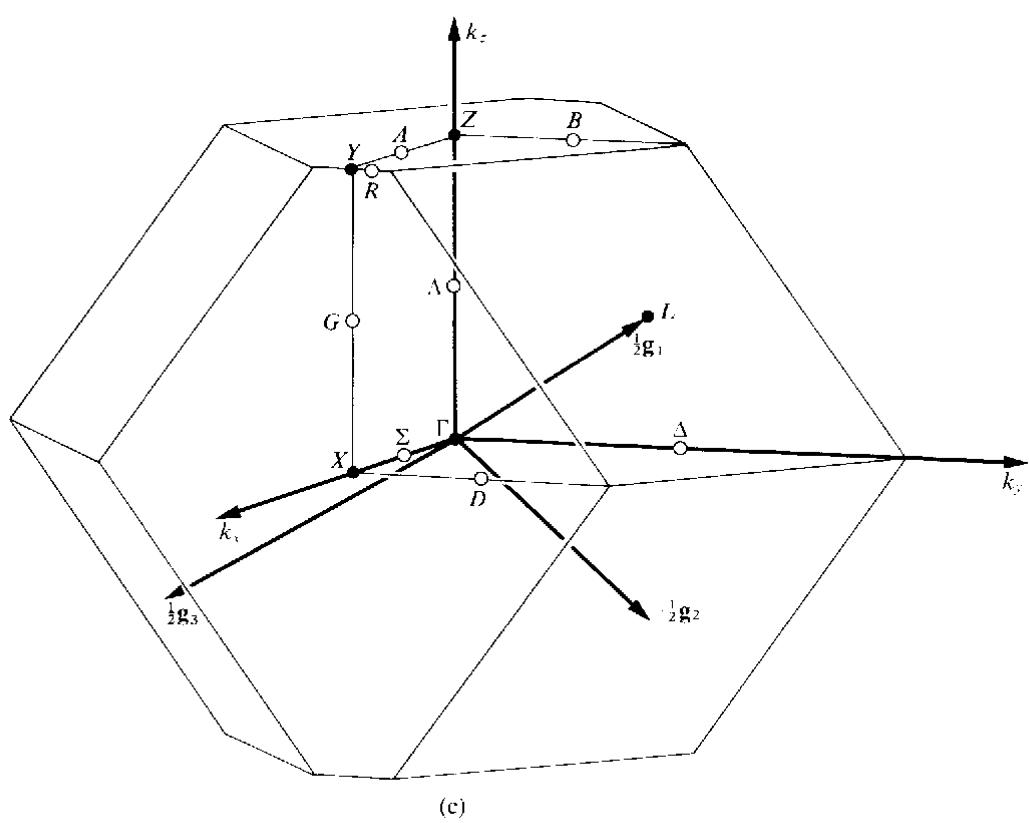
\includegraphics[width=0.60\textwidth]{fig3_8c_mu.jpg}\\[1ex]
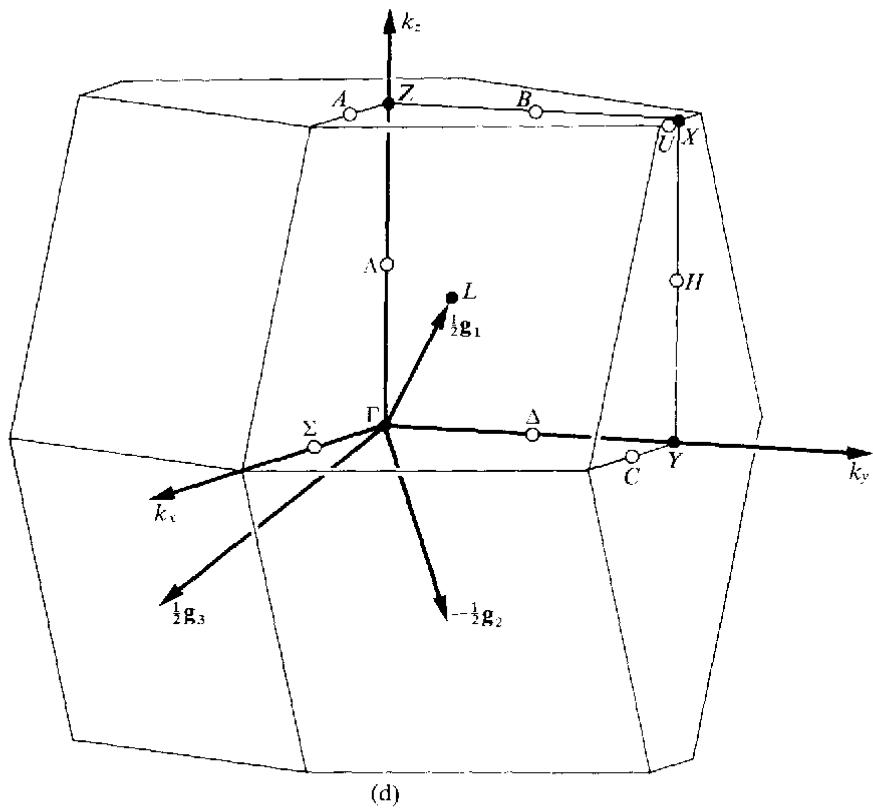
\includegraphics[width=0.60\textwidth]{fig3_8d_mu.jpg}
\caption*{\textbf{图 3.8}\ $\Gamma_{o}^{f}$（正交 $F$）的布里渊区：(a) $1/a^{2}<1/b^{2}+1/c^{2}$、$1/b^{2}<1/c^{2}+1/a^{2}$ 且 $1/c^{2}<1/a^{2}+1/b^{2}$，$\Gamma=(000)$；$Y=(0\bar{\frac{1}{2}}\frac{1}{2})$；$X=(\frac{1}{2}0\frac{1}{2})$；$Z=(\frac{1}{2}\bar{\frac{1}{2}}0)$；$L=(\frac{1}{4}00)$；(b) $1/c^{2}>1/a^{2}+1/b^{2}$，$\Gamma=(000)$；$Y=(0\bar{\frac{1}{2}}\frac{1}{2})$；$X=(\frac{1}{2}0\frac{1}{2})$；$Z=(\frac{1}{2}\bar{\frac{1}{2}}0)$；$L=(\frac{1}{4}00)$；(c) $1/b^{2}>1/a^{2}+1/c^{2}$，$\Gamma=(000)$；$Y=(1\bar{\frac{1}{2}}\frac{1}{2})$；$X=(\frac{1}{2}0\frac{1}{2})$；$Z=(\frac{1}{2}\bar{\frac{1}{2}}0)$；$L=(\frac{1}{4}00)$；(d) $1/a^{2}>1/b^{2}+1/c^{2}$，$\Gamma=(000)$；$Y=(0\bar{\frac{1}{2}}\frac{1}{2})$；$X=(\frac{1}{2}0\frac{1}{2})$；$Z=(\frac{1}{2}\frac{1}{2}0)$；$L=(\frac{1}{4}00)$。}
\end{figure}
\begin{figure}[H]
\centering
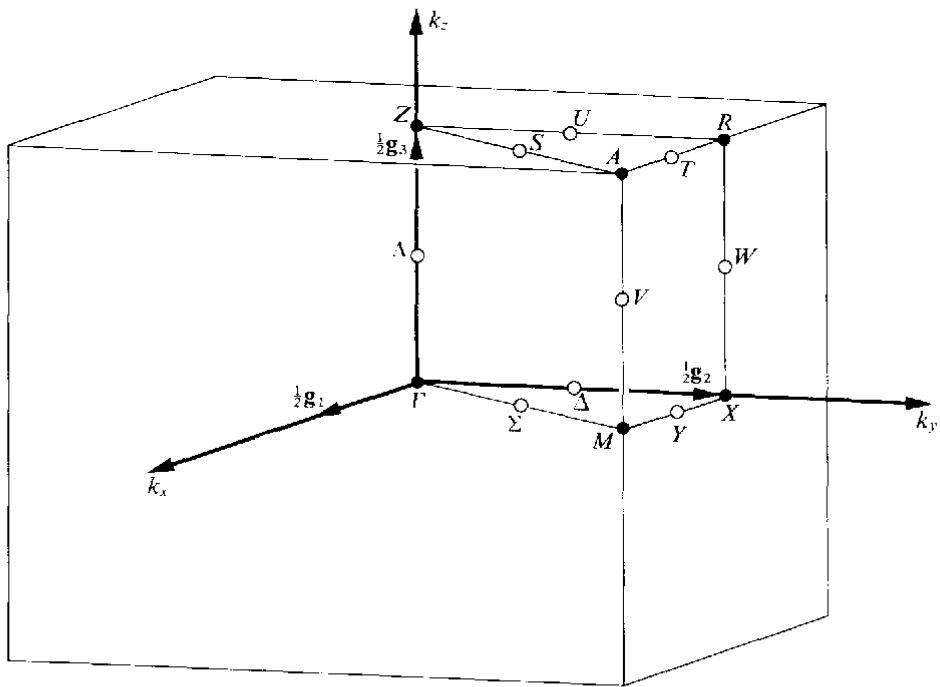
\includegraphics[width=0.60\textwidth]{fig3_9_mu.jpg}
\caption*{\textbf{图 3.9}\ $\Gamma_{q}$（四方 $P$）的布里渊区。$\Gamma=(000)$；$M=(\frac{1}{2}\frac{1}{2}0)$；$Z=(00\frac{1}{2})$；$A=(\frac{1}{2}\frac{1}{2}\frac{1}{2})$；$R=(0\frac{1}{2}\frac{1}{2})$；$X=(0\frac{1}{2}0)$。}
\end{figure}
\begin{figure}[H]
\centering
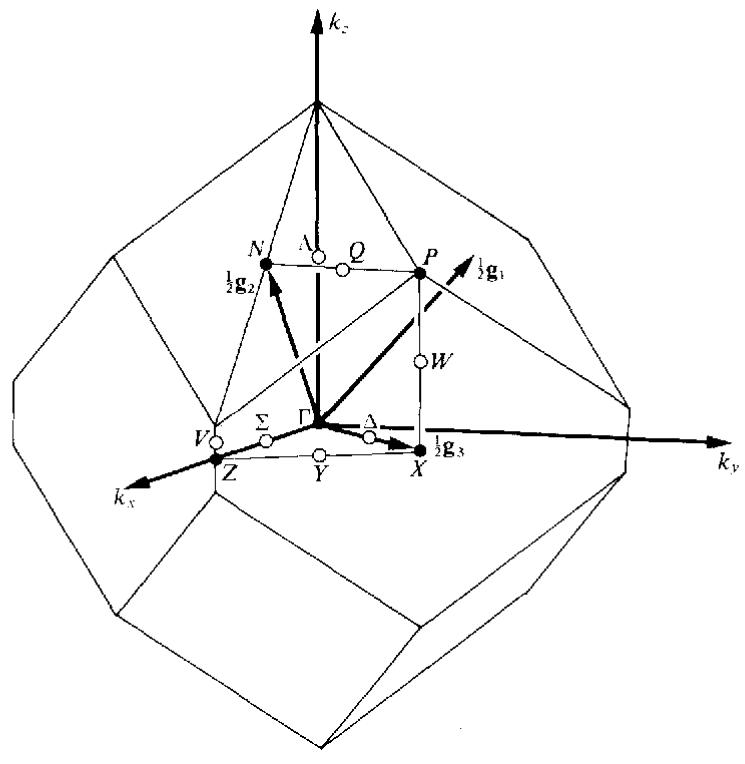
\includegraphics[width=0.60\textwidth]{fig3_10a_mu.jpg}\\[1ex]
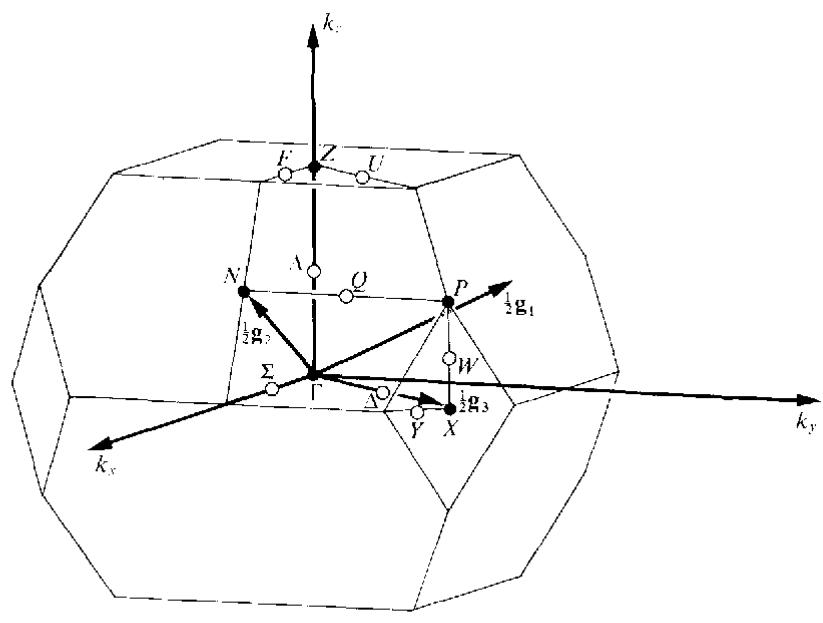
\includegraphics[width=0.60\textwidth]{fig3_10b_mu.jpg}
\caption*{\textbf{图 3.10}\ $\Gamma_{q}^{v}$（四方 $I$）的布里渊区：(a) $a>c$；(b) $c>a$。两种情形都有 $\Gamma=(000)$；$N=(0\frac{1}{2}0)$；$X=(00\frac{1}{2})$；$Z=(\bar{\frac{1}{2}}\bar{\frac{1}{2}}\bar{\frac{1}{2}})$；$P=(\frac{1}{4}\frac{1}{4}\frac{1}{4})$。}
\end{figure}
\begin{figure}[H]
\centering
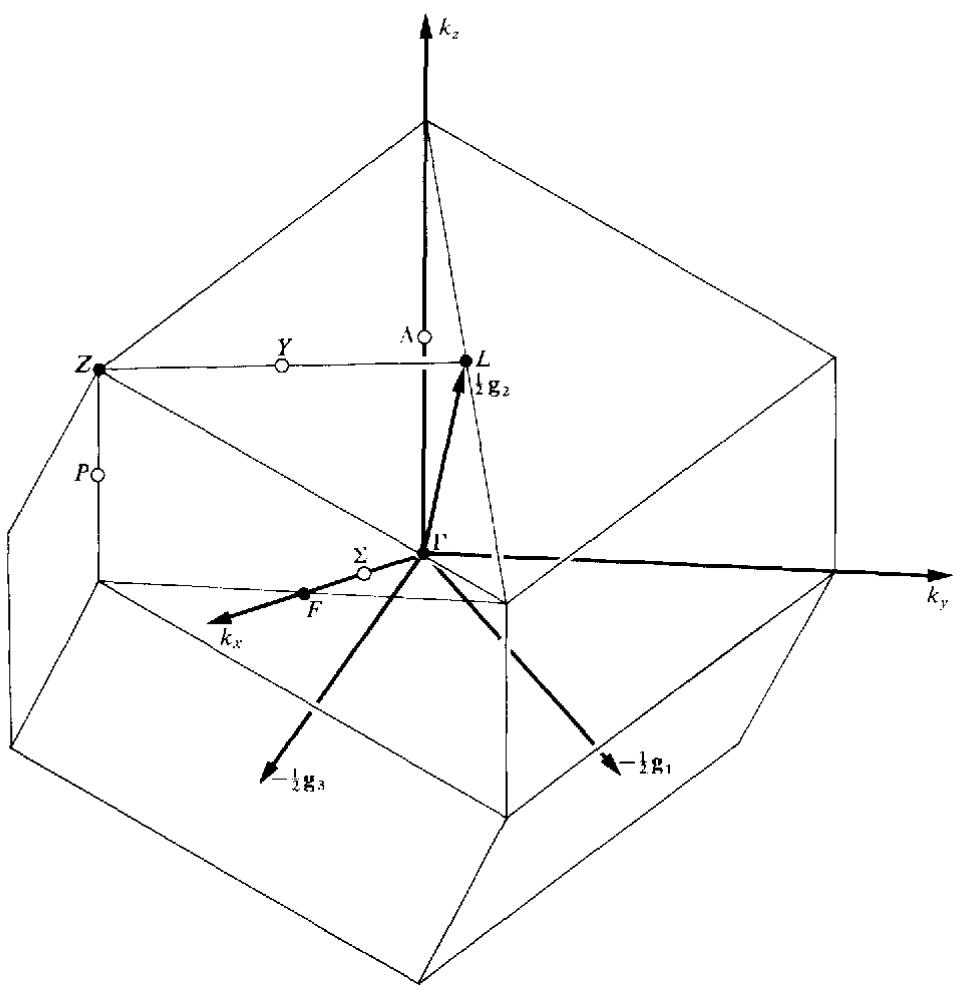
\includegraphics[width=0.60\textwidth]{fig3_11a_mu.jpg}\\[1ex]
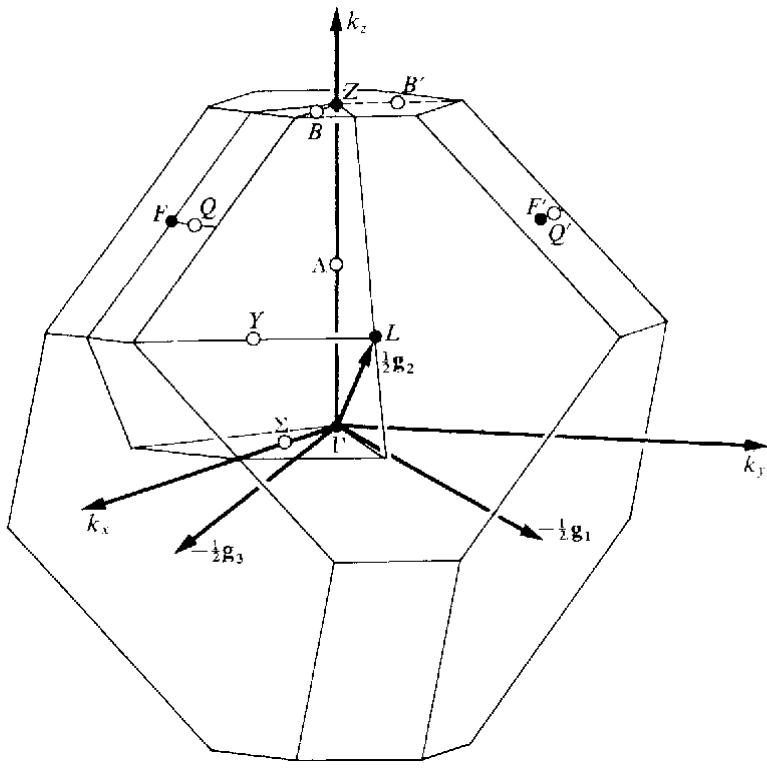
\includegraphics[width=0.60\textwidth]{fig3_11b_mu.jpg}
\caption*{\textbf{图 3.11}\ $\Gamma_{rh}$（三方 $R$）的布里渊区：(a) $a>\sqrt{2}\,c$，$\Gamma=(000)$；$Z=(\frac{1}{2}\frac{1}{2}\bar{\frac{1}{2}})$；$L=(0\frac{1}{2}0)$；$F=(0\frac{1}{2}\bar{\frac{1}{2}})$；(b) $\sqrt{2}\,c>a$，$\Gamma=(000)$；$Z=(\frac{1}{2}\frac{1}{2}\frac{1}{2})$；$L=(0\frac{1}{2}0)$；$F=(\frac{1}{2}\frac{1}{2}0)$。在 (a) 中 $\Sigma$ 和 $Y$ 是两条完整的对称线；在 (b) 中 $Q$ 和 $B$ 经过一个三次转动分别与 $Q'$ 和 $B'$ 相关联，二者分别是线 $\Sigma$ 和 $Y$ 的延续（$F'=(0\bar{\frac{1}{2}}\bar{\frac{1}{2}})$，由 $F$ 经三次转动得到；另见表 3.6）。}
\end{figure}
\begin{figure}[H]
\centering
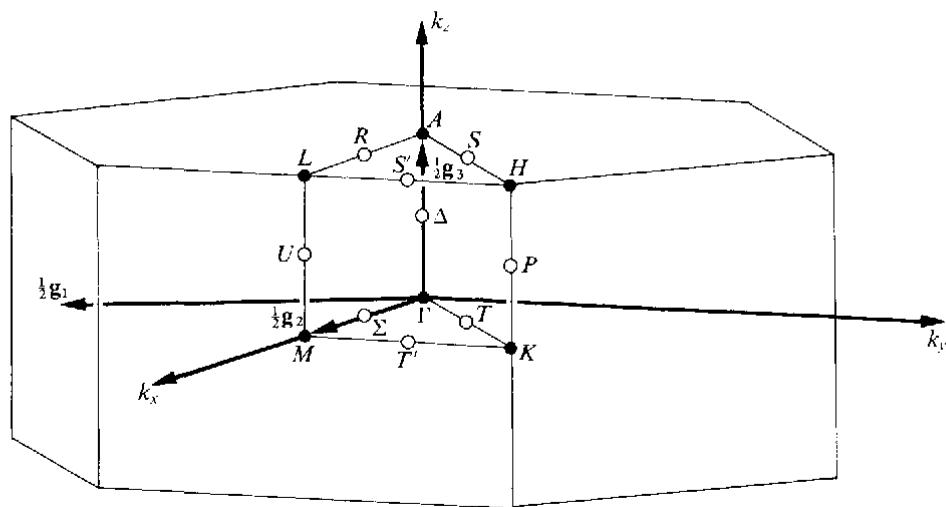
\includegraphics[width=0.60\textwidth]{fig3_12_mu.jpg}
\caption*{\textbf{图 3.12}\ $\Gamma_{h}$（六角 $P$）的布里渊区。$\Gamma=(000)$；$M=(0\frac{1}{2}0)$；$A=(00\frac{1}{2})$；$L=(0\frac{1}{2}\frac{1}{2})$；$K=(\bar{\frac{1}{3}}\frac{2}{3}0)$；$H=(\bar{\frac{1}{3}}\frac{2}{3}\frac{1}{2})$。}
\end{figure}
\begin{figure}[H]
\centering
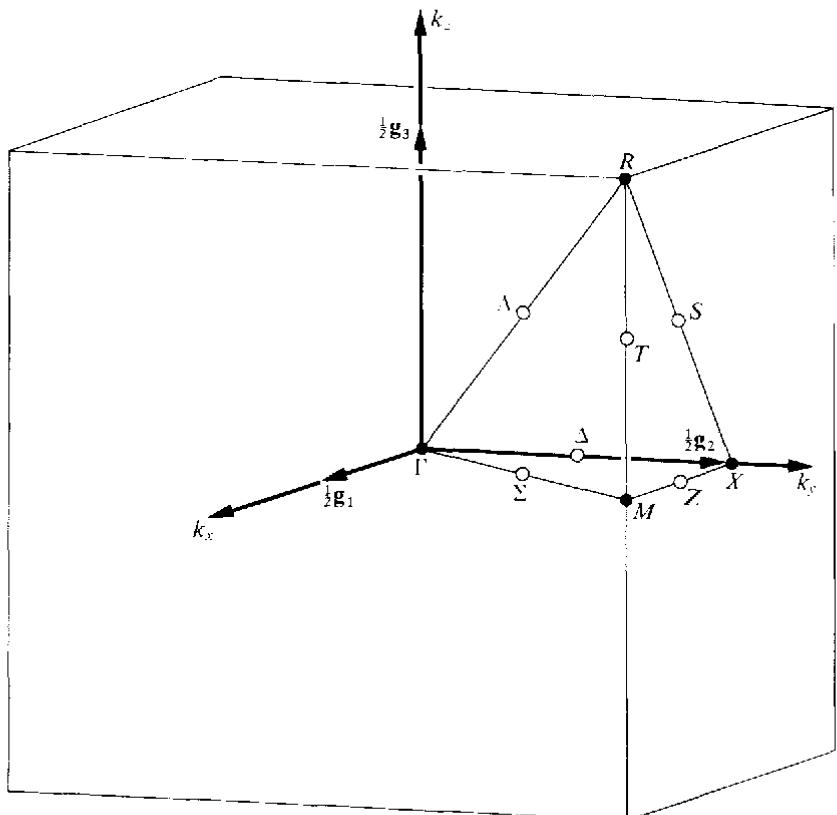
\includegraphics[width=0.58\textwidth]{fig3_13_mu.jpg}
\caption*{\textbf{图 3.13}\ $\Gamma_{c}$（立方 $P$）的布里渊区。$\Gamma=(000)$；$X=(0\frac{1}{2}0)$；$M=(\frac{1}{2}\frac{1}{2}0)$；$R=(\frac{1}{2}\frac{1}{2}\frac{1}{2})$。}
\end{figure}
\begin{figure}[H]
\centering
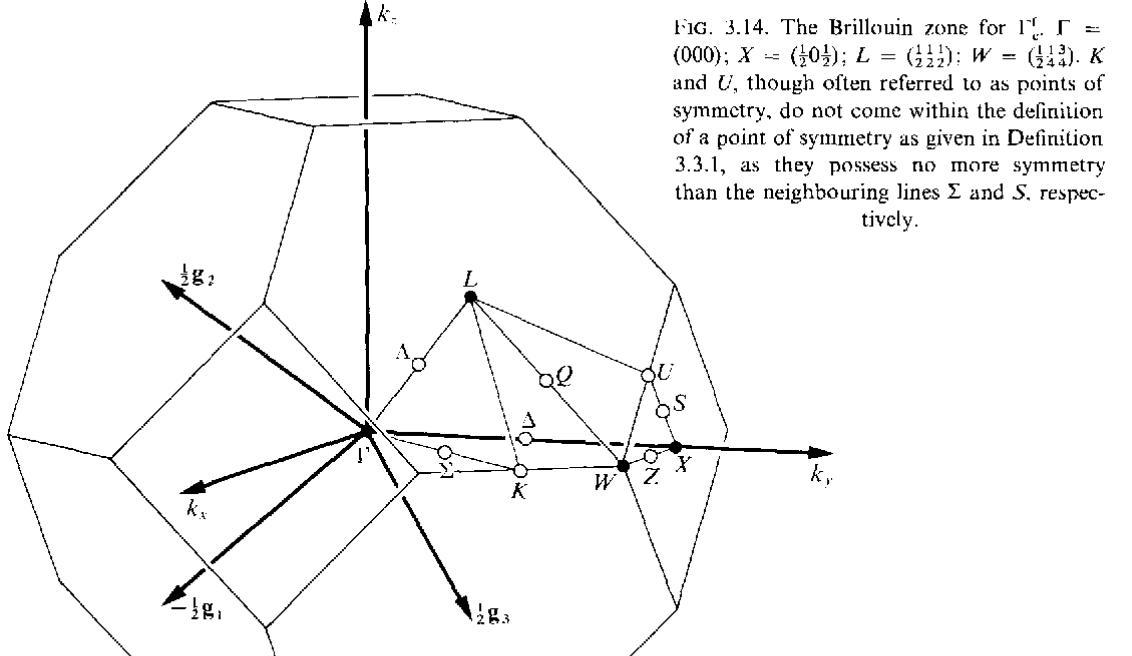
\includegraphics[width=0.58\textwidth]{fig3_14_mu.jpg}
\caption*{\textbf{图 3.14}\ $\Gamma_{c}^{f}$（立方 $F$）的布里渊区。$\Gamma=(000)$；$X=(\frac{1}{2}0\frac{1}{2})$；$L=(\frac{1}{2}\frac{1}{2}\frac{1}{2})$；$W=(\frac{1}{2}\frac{1}{4}\frac{3}{4})$。$K$ 和 $U$ 虽常被称为对称点，但按定义 3.3.1 它们并不算对称点，因为它们并不比相邻的线 $\Sigma$ 和 $S$ 具有更多对称性。}
\end{figure}
\begin{figure}[H]
\centering
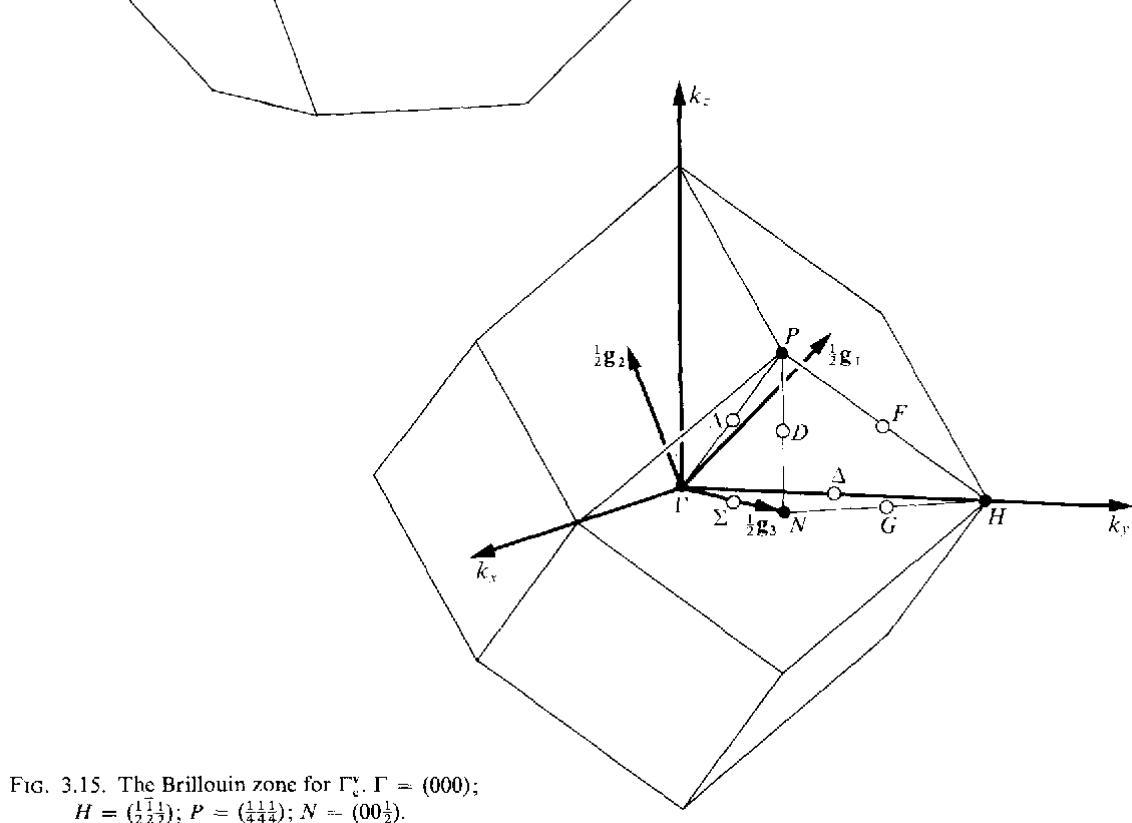
\includegraphics[width=0.56\textwidth]{fig3_15_mu.jpg}
\caption*{\textbf{图 3.15}\ $\Gamma_{c}^{v}$（立方 $I$）的布里渊区。$\Gamma=(000)$；$H=(\frac{1}{2}\frac{1}{2}\frac{1}{2})$；$P=(\frac{1}{4}\frac{1}{4}\frac{1}{4})$；$N=(00\frac{1}{2})$。}
\end{figure}

对某些布拉维格子，布里渊区的形状是唯一的，例如三种立方布拉维格子（其布里渊区绘于图 3.13--3.15）。但对另外一些布拉维格子，可能出现的形状不止一种，取决于布拉维格子的轴比和轴间角。对三斜布拉维格子（图 3.2）和两种单斜布拉维格子（图 3.3、3.4），我们遵循定义 3.2.2，用倒空间的初基晶胞来定义布里渊区。对另一些布拉维格子，可能出现表面上不同的布里渊区（例如图 3.8 的 $\Gamma_{o}^{f}$、图 3.10 的 $\Gamma_{q}^{v}$、图 3.11 的 $\Gamma_{rh}$）。然而，当可能有两个表面上不同的布里渊区时，每种情形中对称点的数目是相同的。例如在图 3.11(a)（$\Gamma_{rh}$，$a>\sqrt{2}\,c$）中，对称点是 $\Gamma$（$\mathbf{k}=0$）、$L$（$\mathbf{k}=\frac{1}{2}\mathbf{g}_{2}$）、$F$（$\mathbf{k}=\frac{1}{2}\mathbf{g}_{2}-\frac{1}{2}\mathbf{g}_{3}$）和 $Z$（$\mathbf{k}=\frac{1}{2}\mathbf{g}_{1}+\frac{1}{2}\mathbf{g}_{2}-\frac{1}{2}\mathbf{g}_{3}$）；而在图 3.11(b) 的替代布里渊区（$a<\sqrt{2}\,c$）中，对称点是 $\Gamma$（$\mathbf{k}=0$）、$L$（$\mathbf{k}=\frac{1}{2}\mathbf{g}_{2}$）、$F$（$\mathbf{k}=\frac{1}{2}\mathbf{g}_{1}+\frac{1}{2}\mathbf{g}_{2}$）和 $Z$（$\mathbf{k}=\frac{1}{2}\mathbf{g}_{1}+\frac{1}{2}\mathbf{g}_{2}+\frac{1}{2}\mathbf{g}_{3}$）。$\Gamma$ 和 $L$ 在两个布里渊区中以相同的 $\mathbf{k}$ 出现，而图 3.11(a) 中的 $F$ 和 $Z$ 在图 3.11(b) 中对应的 $\mathbf{k}$ 矢量不同但等价。对另外一些布拉维格子，布里渊区的外形相同，只是各面相对 $k_{x}$、$k_{y}$、$k_{z}$ 轴的取向不同，见图 3.16。

\begin{figure}[H]
\centering
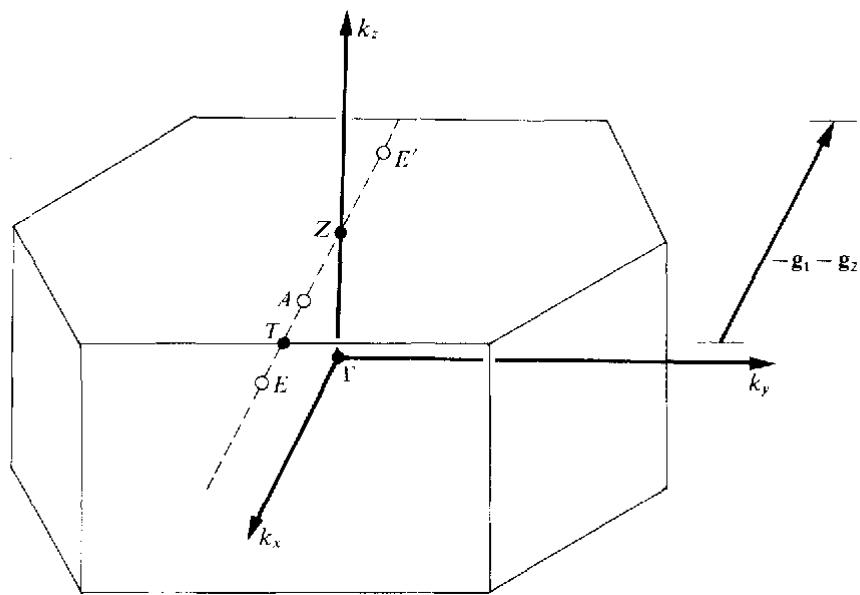
\includegraphics[width=0.56\textwidth]{fig3_16_mu.jpg}
\caption*{\textbf{图 3.16}\ $\Gamma_{o}^{b}$ 的布里渊区。}
\end{figure}

考虑 $\Gamma_{o}^{b}$（图 3.6）。当 $a>b$ 时（图 3.6(a)），设 $T$ 是线 $ZT$ 上的一个点，其 $\mathbf{k}$ 矢量为 $\mathbf{k}_{T}$，则
\begin{equation*}
\mathbf{k}_{E} = \mathbf{k}_{T} + (\alpha\mathbf{g}_{1} + \alpha\mathbf{g}_{2}).
\tag{3.3.2}
\end{equation*}
图 3.6(a) 中相应的对称线具有由式 (3.3.2) 给出的 $\mathbf{k}$ 矢量 $\mathbf{k}_{E}$，即线 $ZT$ 的延续；见图 3.16。这条线 $E$ 现在已跑到第一布里渊区之外，但它等价于第一区内的一条线，即 $E'$，其中
\begin{equation*}
\mathbf{k}_{E'} = \mathbf{k}_{E} - \mathbf{g}_{1} - \mathbf{g}_{2}.
\tag{3.3.3}
\end{equation*}
线 $E'$ 与图 3.6(a) 中的线 $A$ 有简单的对称关系，因此不必把它同 $A$ 分开考虑。反过来看，这意味着图 3.6(a) 中的线 $A$ 在图 3.6(b) 中被分成两段：对某些 $\alpha$ 值的一段是图 3.6(a) 的 $A$，对其余 $\alpha$ 值的一段是图 3.6(b) 的 $E$。类似地，图 3.6(a) 中的线 $\Sigma$ 在图 3.6(b) 中被分成 $\Lambda$ 和 $C$。反过来，图 3.6(b) 中的线 $A$ 在图 3.6(a) 中被分成 $\Delta$ 和 $F$，而图 3.6(b) 中的线 $B$ 被分成 $\Delta$ 和 $F'$。

由于我们指出的这种等价性，在本书后面的表中，对 14 种布拉维格子中的每一种，只需对一个布里渊区列出对称点即可；通常也只需对每一种格子列出一张对称线表。不过，对区面上的对称线存在少数例外。例如，虽然图 3.6(b) 中的 $C$ 与图 3.6(a) 中的 $E$ 相关联，但二者之间存在一个微妙的差别，这将在后文变得明显。

14 种布拉维格子各自基本域中每个对称点和对称线的群 $\mathbf{P}(\mathbf{k})$（$\mathbf{k}$ 的对称群）列于表 3.6。可以注意到，图 3.2--3.15 中基本域的许多棱并不是对称线，而只是（按定义 3.3.2 的意义）对称面。把我们限制在单一基本域的理由后文自明；例如见 5.5 节。

\begin{figure}[H]
\centering
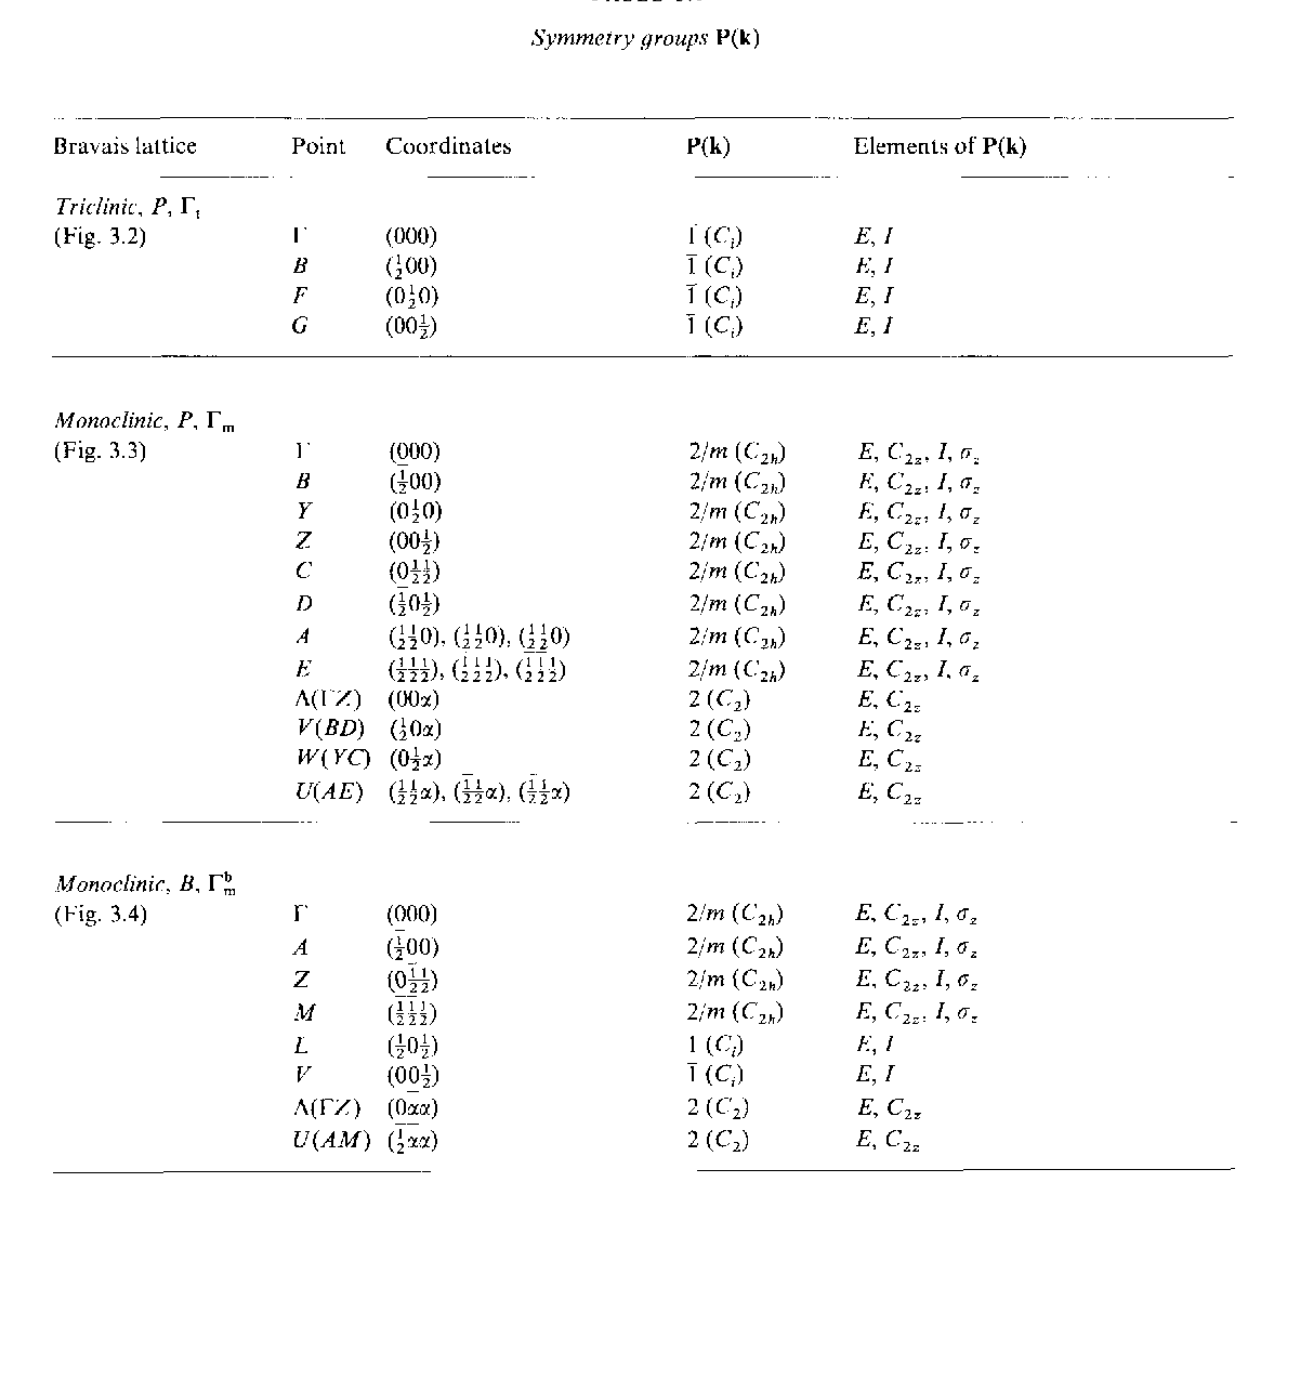
\includegraphics[width=0.92\textwidth]{c3_t36_p1.png}
\caption*{\textbf{表 3.6}\ 对称群 $\mathbf{P}(\mathbf{k})$（原书第 113 页起扫描；第 1--5 页）。}
\end{figure}
\begin{figure}[H]
\centering
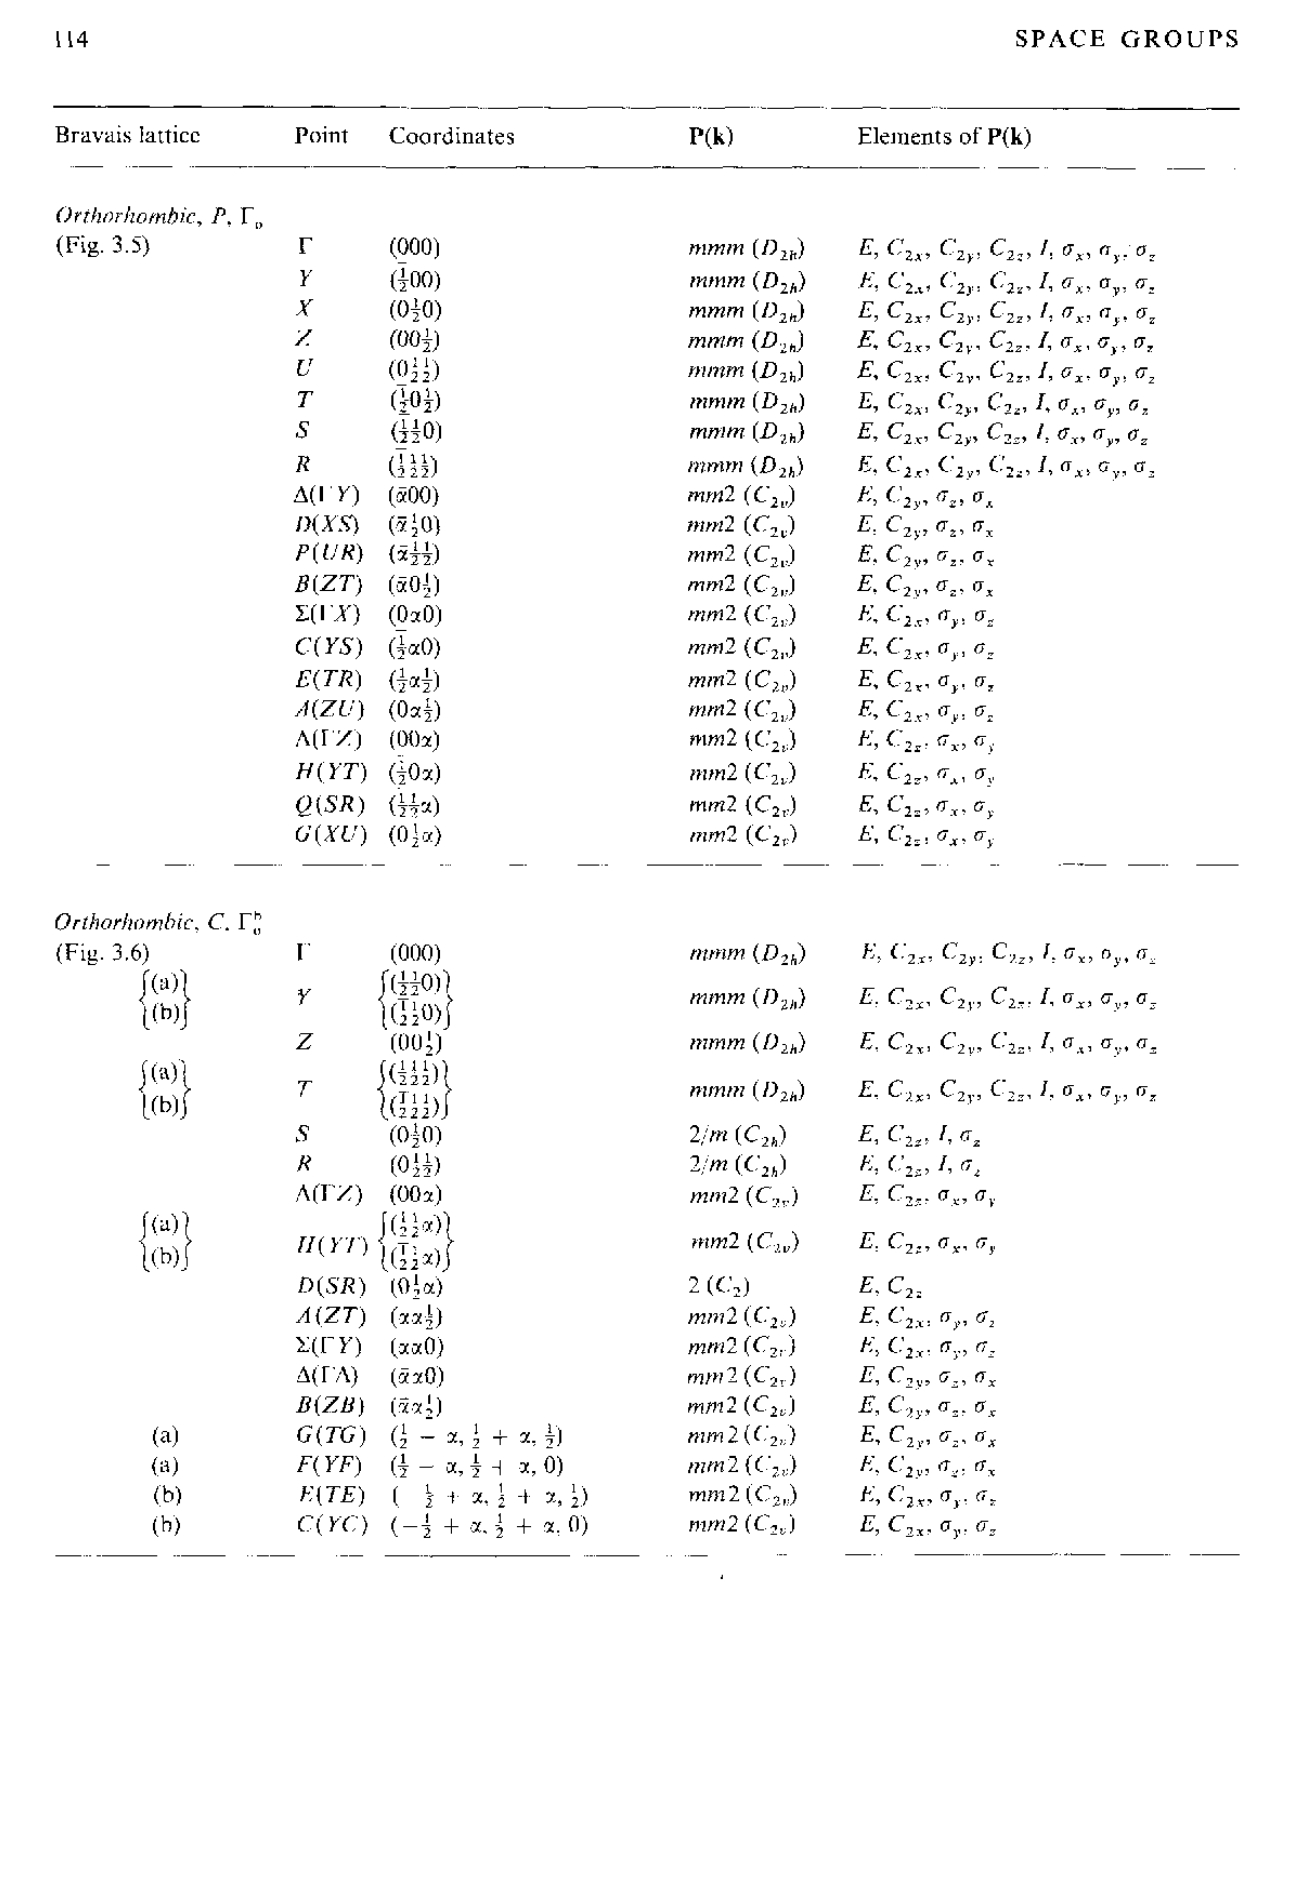
\includegraphics[width=0.92\textwidth]{c3_t36_p2.png}
\caption*{\textbf{表 3.6}（第 2 页）。}
\end{figure}
\begin{figure}[H]
\centering
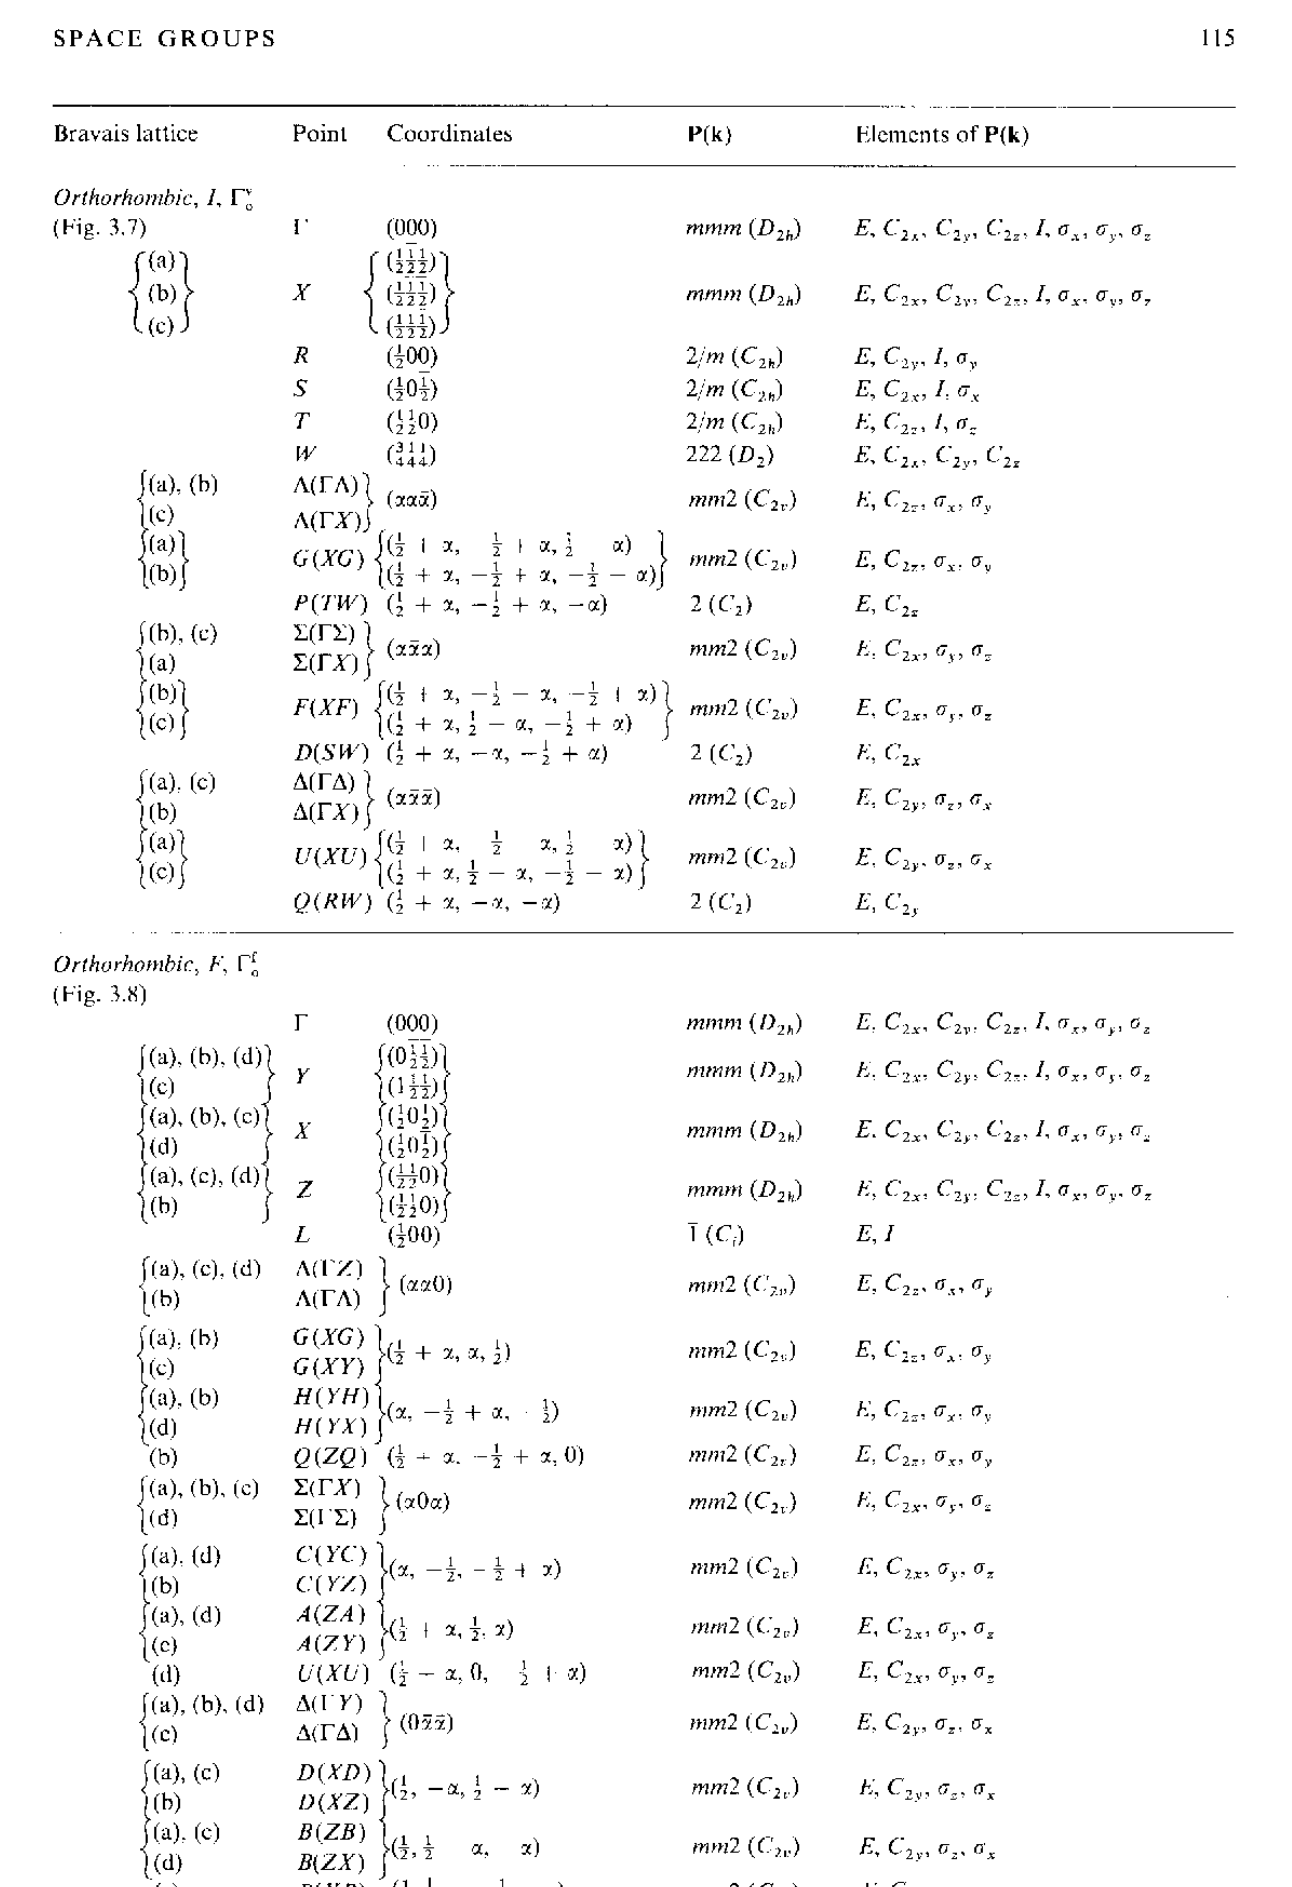
\includegraphics[width=0.92\textwidth]{c3_t36_p3.png}
\caption*{\textbf{表 3.6}（第 3 页）。}
\end{figure}
\begin{figure}[H]
\centering
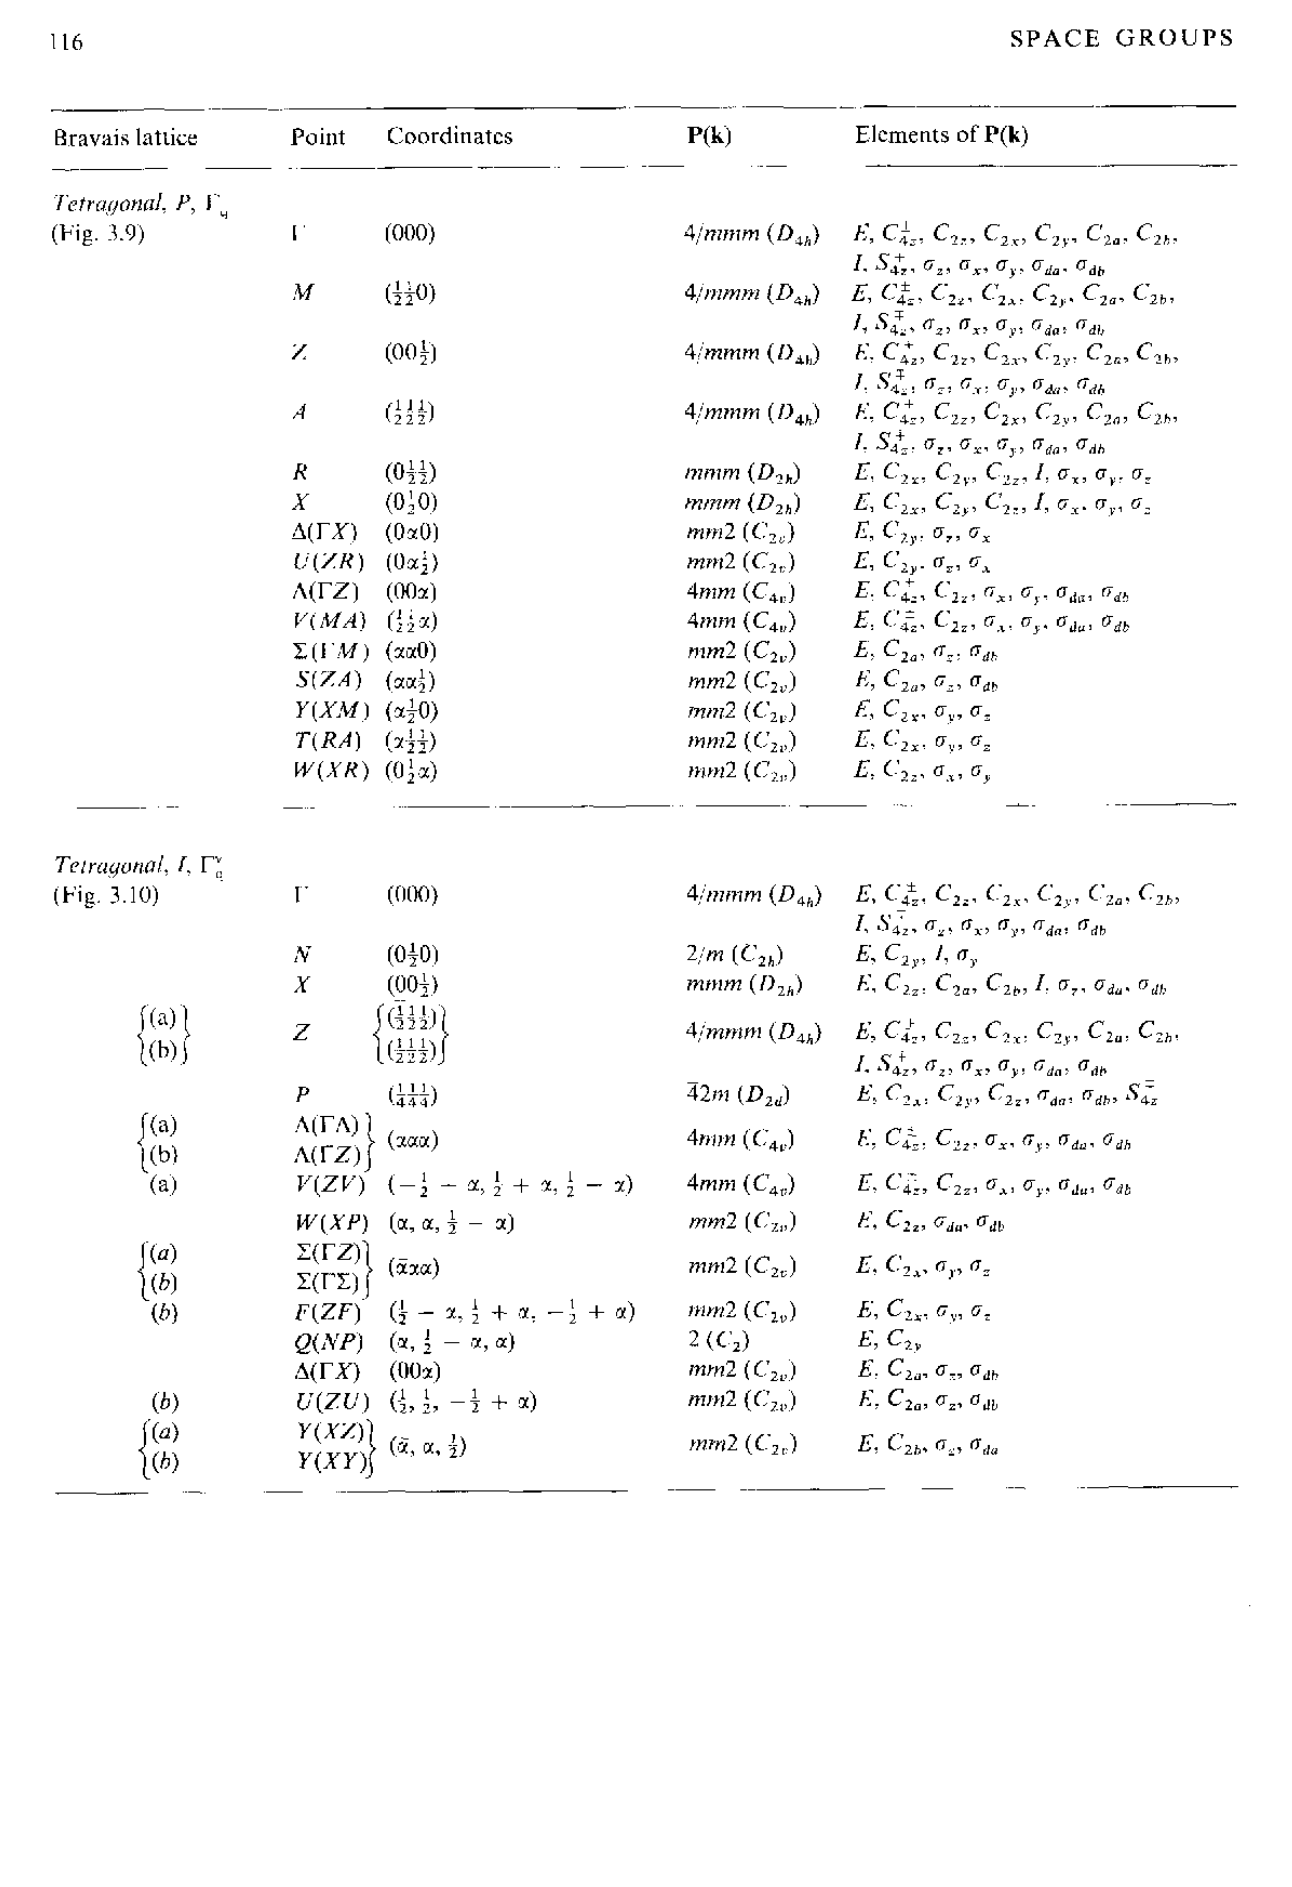
\includegraphics[width=0.92\textwidth]{c3_t36_p4.png}
\caption*{\textbf{表 3.6}（第 4 页）。}
\end{figure}
\begin{figure}[H]
\centering
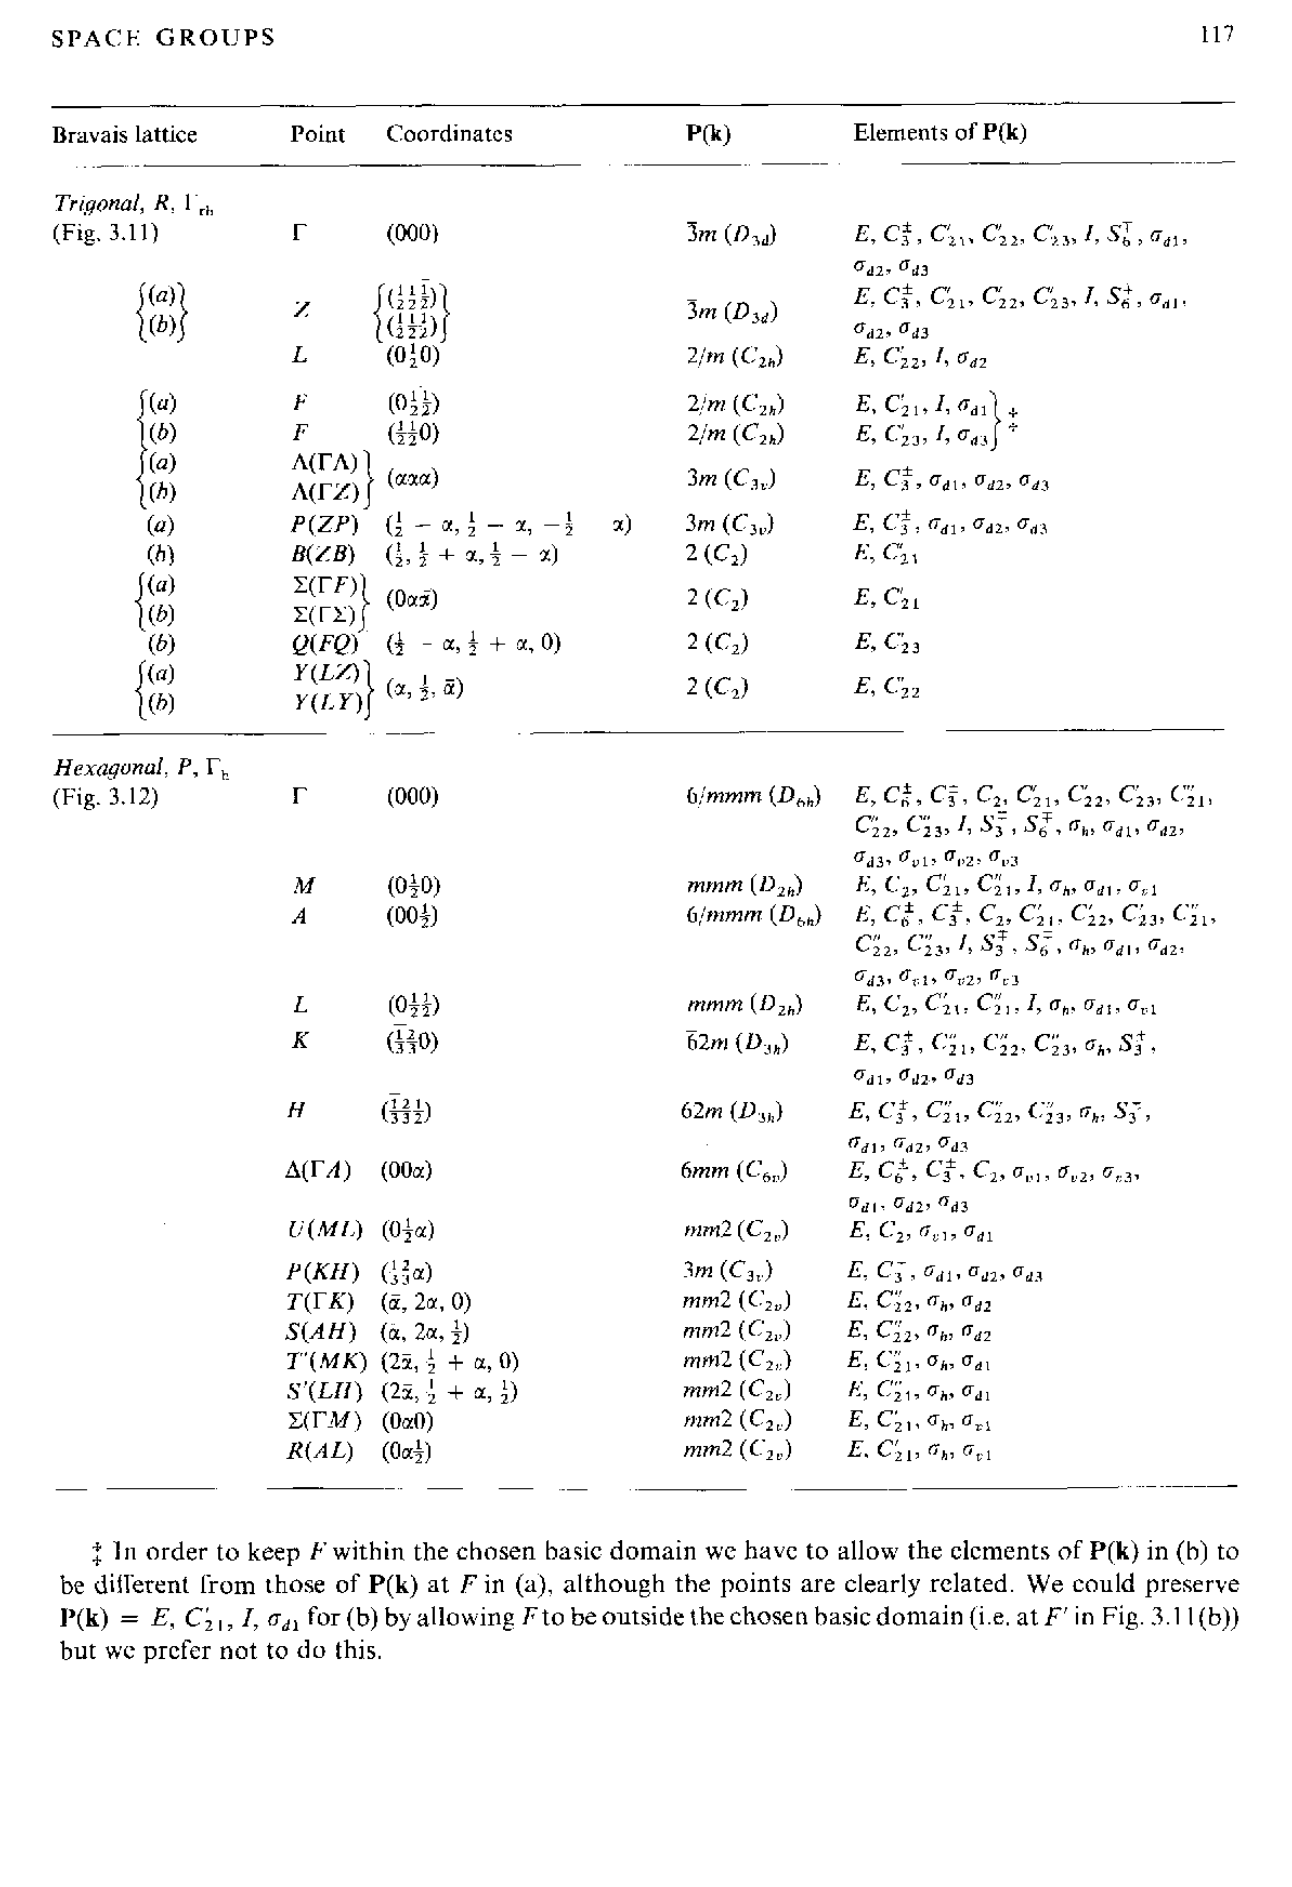
\includegraphics[width=0.92\textwidth]{c3_t36_p5.png}
\caption*{\textbf{表 3.6}（第 5 页；本页下部有关于 $\Gamma_{rh}$ 的 $F$ 点的脚注）。}
\end{figure}
\begin{figure}[H]
\centering
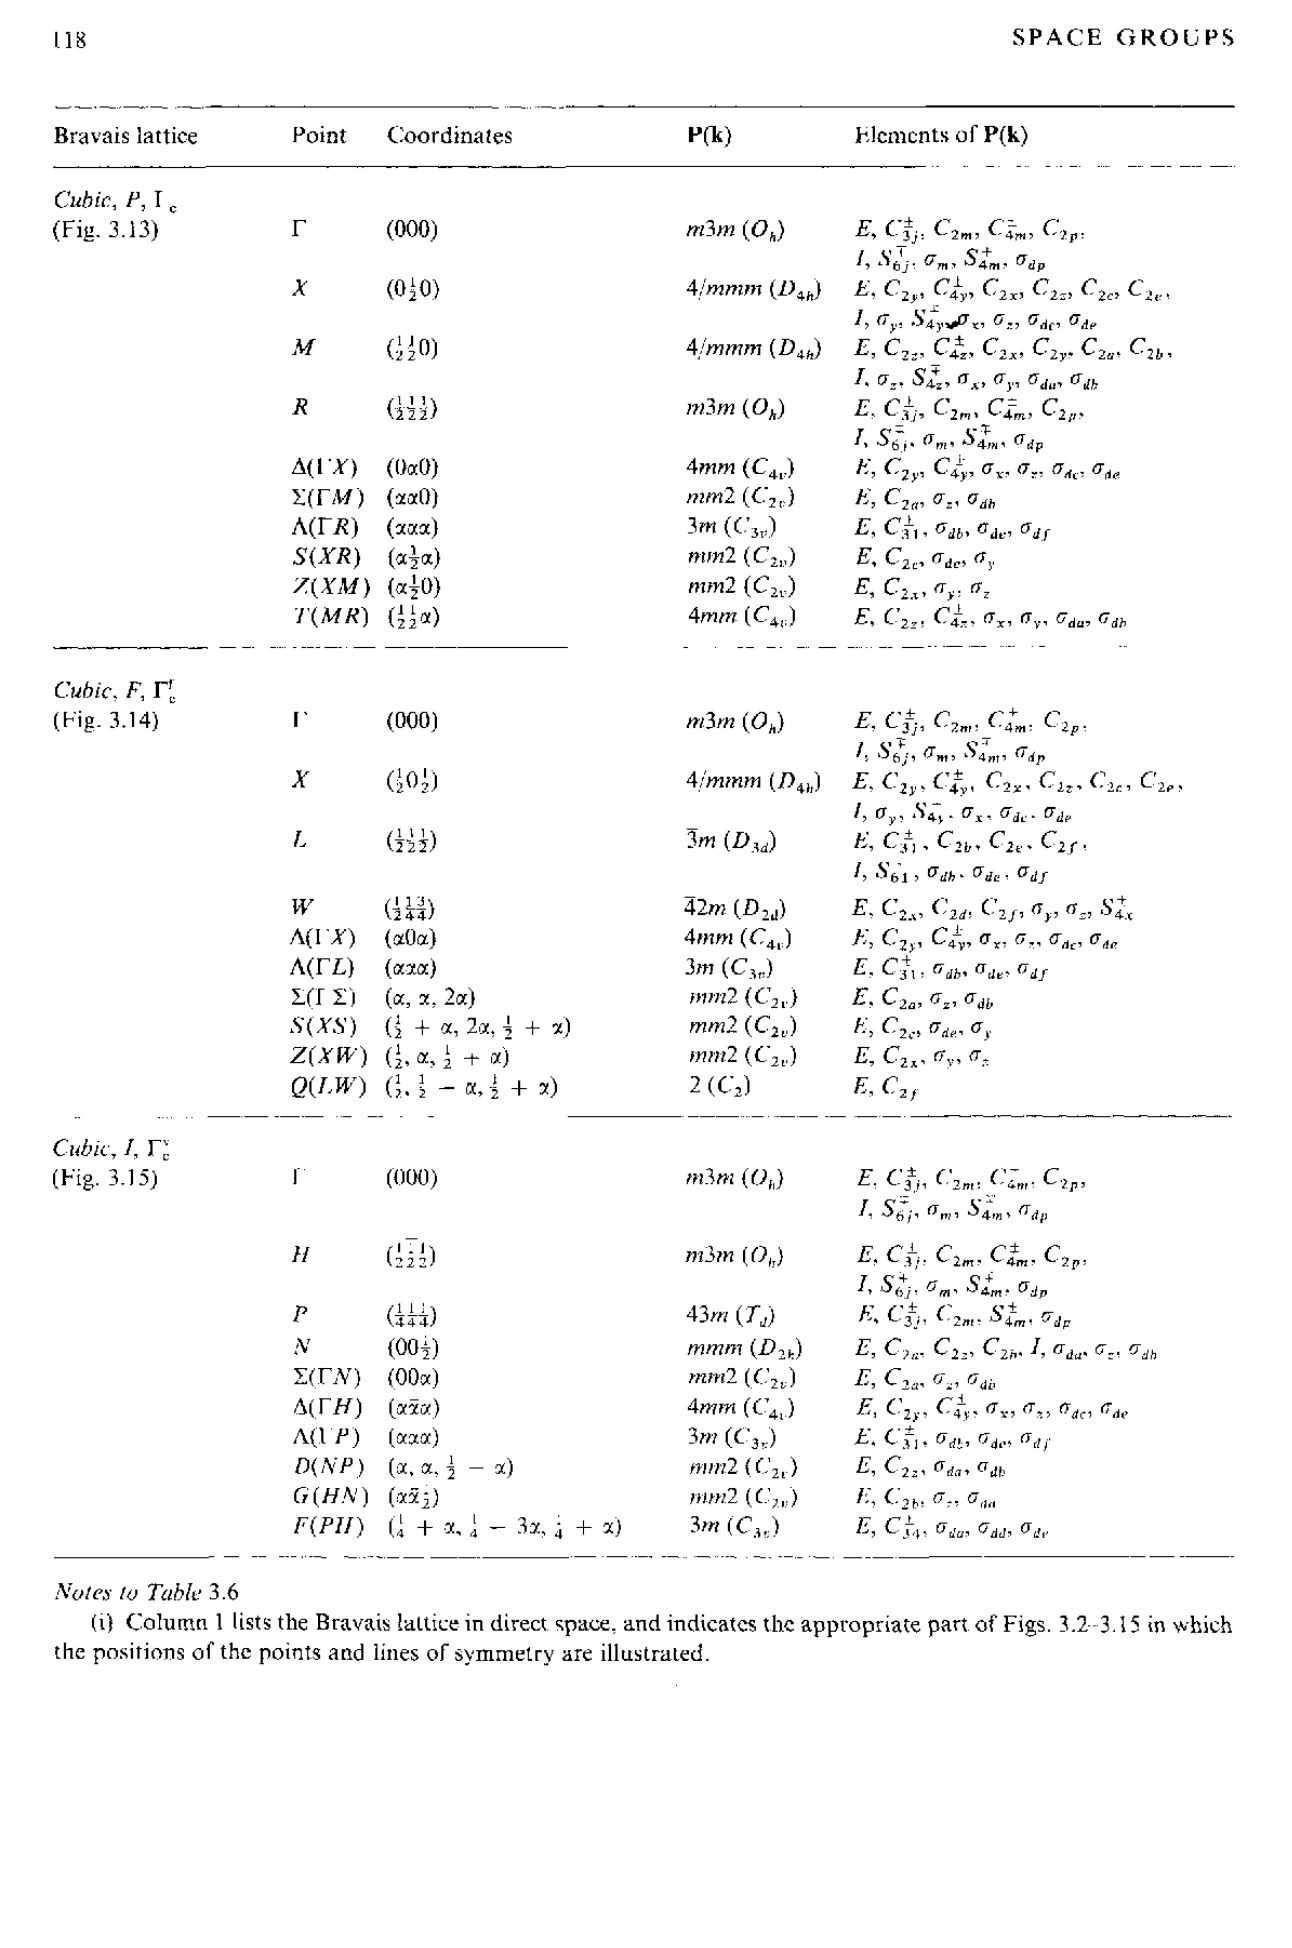
\includegraphics[width=0.92\textwidth]{c3_t36_p6.png}
\caption*{\textbf{表 3.6}（第 6 页，立方 $P$、$F$、$I$；页末起为表的注）。}
\end{figure}
\begin{figure}[H]
\centering
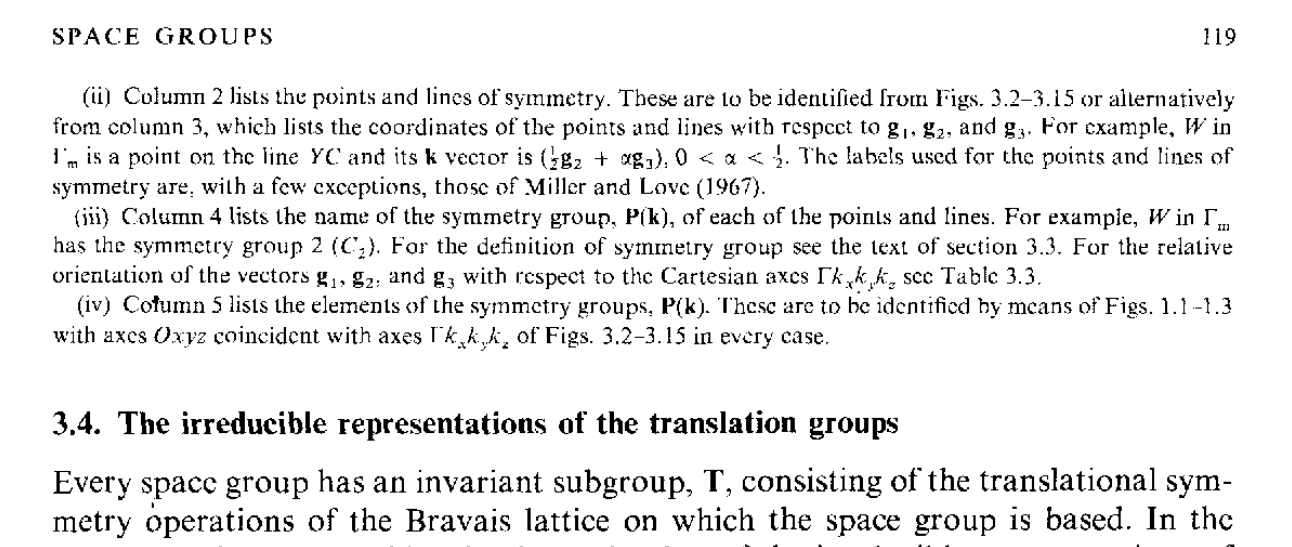
\includegraphics[width=0.92\textwidth]{c3_t36_p7.png}
\caption*{\textbf{表 3.6}（注 (ii)--(iv)，原书扫描占位）。}
\end{figure}

表 3.6 的注（译文）：

\noindent（i）第 1 列列出正空间的布拉维格子，并指出图 3.2--3.15 中展示各对称点和对称线位置的相应部分。

\noindent（ii）第 2 列列出对称点和对称线。它们既可从图 3.2--3.15 辨认，也可从第 3 列辨认；第 3 列列出各点和线相对于 $\mathbf{g}_{1}$、$\mathbf{g}_{2}$、$\mathbf{g}_{3}$ 的坐标。例如 $\Gamma_{m}$ 中的 $W$ 是线 $YC$ 上的一个点，其 $\mathbf{k}$ 矢量为 $\frac{1}{2}\mathbf{g}_{2}+\alpha\mathbf{g}_{3}$（$0<\alpha<\frac{1}{2}$）。对称点和对称线所用的标记，除少数例外，都是 Miller and Love（1967）的记号。

\noindent（iii）第 4 列列出各点和线的对称群 $\mathbf{P}(\mathbf{k})$ 的名称。例如 $\Gamma_{m}$ 中的 $W$ 具有对称群 $2\ (C_{2})$。对称群的定义见 3.3 节正文。矢量 $\mathbf{g}_{1}$、$\mathbf{g}_{2}$、$\mathbf{g}_{3}$ 相对于笛卡尔轴 $\Gamma k_{x}k_{y}k_{z}$ 的取向见表 3.3。

\noindent（iv）第 5 列列出对称群 $\mathbf{P}(\mathbf{k})$ 的元素。这些元素可借助图 1.1--1.3 来辨认，此时在所有情形下都取 $Oxyz$ 轴与图 3.2--3.15 的 $\Gamma k_{x}k_{y}k_{z}$ 轴重合。

\noindent（关于表中 $\Gamma_{rh}$ 的 $F$ 点的脚注：为了把 $F$ 保持在所选的基本域内，不得不让 (b) 中 $F$ 的 $\mathbf{P}(\mathbf{k})$ 元素与 (a) 中 $F$ 的不同，尽管这两个点显然是互相关联的。若允许 $F$ 位于所选基本域之外（即位于图 3.11(b) 的 $F'$ 处），本可使二者一致，但我们不拟这样做。）

% 3.4 平移群的不可约表示
\section{平移群的不可约表示}

每个空间群都有一个不变子群 $\mathbf{T}$，它由空间群所依托的布拉维格子的平移对称操作构成。本节考虑如何确定布拉维格子的平移对称操作群的不可约表示。

$\mathbf{T}$ 由元素 $\{E \mid n_{1}\mathbf{t}_{1} + n_{2}\mathbf{t}_{2} + n_{3}\mathbf{t}_{3}\}$ 构成，其中 $n_{i}$ 是满足 $0 \leqslant n_{i} < N_{i}$（$i = 1, 2$ 或 3）的整数，并且施加 Born--von Kármán 循环边界条件（Born and von Kármán 1913\textit{a}, \textit{b}）。由于乘法规则形如 $\{E \mid \mathbf{t}\}\{E \mid \mathbf{s}\} = \{E \mid \mathbf{t} + \mathbf{s}\}$，又由于式 (3.1.1) 所施加的周期性，$\mathbf{T}$ 是三个阶分别为 $N_{1}$、$N_{2}$、$N_{3}$ 的循环群的外直积，于是用明显的记号可以写 $\mathbf{T} = \mathbf{T}_{1} \otimes \mathbf{T}_{2} \otimes \mathbf{T}_{3}$。循环群的表示是众所周知的。例如，$\mathbf{T}_{1}$ 的表示 $\Delta$ 共有 $N_{1}$ 个，每一个用整数 $p_{1}$（$0 \leqslant p_{1} < N_{1}$）标记，使得
\begin{equation*}
\Delta^{p_{1}}(\{E \mid n_{1}\mathbf{t}_{1}\}) = \exp(-2\pi\mathrm{i}\, n_{1}p_{1}/N_{1}).
\tag{3.4.1}
\end{equation*}
由直积群上的定理 (1.3.16)，现在可以容易地导出 $\mathbf{T}$ 的表示。它们都是一维的，共 $N_{1}N_{2}N_{3}$ 个。每个表示用三个整数 $p_{1}$、$p_{2}$、$p_{3}$（$0 \leqslant p_{i} < N_{i}$）标记。若写 $k_{i} = p_{i}/N_{i}$，则可取 $\mathbf{k} = (k_{1}, k_{2}, k_{3})$ 为倒空间中的一个矢量，即
\begin{equation*}
\mathbf{k} = k_{1}\mathbf{g}_{1} + k_{2}\mathbf{g}_{2} + k_{3}\mathbf{g}_{3}.
\tag{3.4.2}
\end{equation*}
于是 $\mathbf{k}$ 可以拿来作为 $\mathbf{T}$ 的表示的标记，这些表示就是
\begin{equation*}
\Delta^{\mathbf{k}}\left[\{E \mid n_{1}\mathbf{t}_{1} + n_{2}\mathbf{t}_{2} + n_{3}\mathbf{t}_{3}\}\right] = \exp\left\{-\mathrm{i}\,\mathbf{k} \cdot (n_{1}\mathbf{t}_{1} + n_{2}\mathbf{t}_{2} + n_{3}\mathbf{t}_{3})\right\}.
\tag{3.4.3}
\end{equation*}
现在我们可以看出，为什么在定义中把相差一个倒格子矢量的两个 $\mathbf{k}$ 矢量称为等价。因为若 $\mathbf{k}' = \mathbf{k} + \mathbf{g}$，则由于 $\exp(-\mathrm{i}\,\mathbf{g} \cdot \mathbf{t}) = 1$，
\begin{equation*}
\Delta^{\mathbf{k}'}(\mathbf{t}) = \exp\left\{-\mathrm{i}(\mathbf{k} + \mathbf{g}) \cdot \mathbf{t}\right\} = \Delta^{\mathbf{k}}(\mathbf{t}).
\tag{3.4.4}
\end{equation*}
因此，可以取任意 $N_{1}N_{2}N_{3}$ 个互不等价的 $\mathbf{k}$ 矢量作为 $\mathbf{k}$ 的允许值。上面定义的那一组就是这样一组矢量，它们的终点落在倒空间初基晶胞的内部或表面上（除原点的移动之外）；对三斜和单斜布拉维格子，我们正是用这个初基晶胞来定义布里渊区的（见定义 3.2.2）。对所有其他布拉维格子，可以取终点落在倒空间 Wigner--Seitz 晶胞内部或表面上的那一组矢量作为 $N_{1}N_{2}N_{3}$ 个非等价的 $\mathbf{k}$ 矢量（见定义 3.2.1）。这样，在任何情形下我们都可以把 $\mathbf{T}$ 的表示看作由布里渊区的点 $\mathbf{k}$ 所定义的。

有一个关于允许的 $\mathbf{k}$ 矢量密度的公式会很有用。在体积 $8\pi^{3}/V$（$V$ 是晶体晶胞的体积）中共有 $N_{1}N_{2}N_{3}$ 个 $\mathbf{k}$ 矢量。因此密度 $n(\mathbf{k})$ 为 $N_{1}N_{2}N_{3}V/8\pi^{3} = W/8\pi^{3}$，其中 $W$ 是晶体的体积。于是
\begin{equation*}
n(\mathbf{k}) = \frac{W}{8\pi^{3}}.
\tag{3.4.5}
\end{equation*}
这意味着，在无穷晶体的极限下，$\mathbf{k}$ 的取值变得任意接近，从而稠密地填满整个布里渊区。

$\Delta^{\mathbf{k}}$ 的基函数可以取 $\exp(\mathrm{i}\mathbf{k} \cdot \mathbf{r})$，因为由例 1.5.3，
\begin{equation*}
\begin{aligned}
\{E \mid \mathbf{t}\}\exp(\mathrm{i}\mathbf{k} \cdot \mathbf{r}) &= \exp\left\{\mathrm{i}\mathbf{k} \cdot (\mathbf{r} - \mathbf{t})\right\} \\
&= \exp(-\mathrm{i}\mathbf{k} \cdot \mathbf{t})\exp(\mathrm{i}\mathbf{k} \cdot \mathbf{r}) = \Delta^{\mathbf{k}}\{E \mid \mathbf{t}\}\exp(\mathrm{i}\mathbf{k} \cdot \mathbf{r}).
\end{aligned}
\tag{3.4.6}
\end{equation*}
代替 $\exp(\mathrm{i}\mathbf{k} \cdot \mathbf{r})$，我们可以使用任何形如
\begin{equation*}
\Psi_{\mathbf{k}}(\mathbf{r}) = \exp(\mathrm{i}\mathbf{k} \cdot \mathbf{r})\,u_{\mathbf{k}}(\mathbf{r})
\tag{3.4.7}
\end{equation*}
的函数，其中
\begin{equation*}
u_{\mathbf{k}}(\mathbf{r}) = u_{\mathbf{k}}(\mathbf{r} + \mathbf{t})
\tag{3.4.8}
\end{equation*}
对一切 $\mathbf{t}$ 成立。平移群 $\mathbf{T}$ 的基函数具有式 (3.4.7) 与 (3.4.8) 所定义的形式，这一结论通常称为 Bloch 定理。

\noindent\textbf{定理 3.4.1}\quad （Bloch 定理）（Bloch 1928）\ 在由 $\mathbf{T}$ 定义其周期性的周期性势场 $V(\mathbf{r})$ 中运动的粒子或准粒子的波函数可以写成
\begin{equation*}
\Psi_{\mathbf{k}}(\mathbf{r}) = \exp(\mathrm{i}\mathbf{k} \cdot \mathbf{r})\,u_{\mathbf{k}}(\mathbf{r})
\tag{3.4.7}
\end{equation*}
的形式，其中 $u_{\mathbf{k}}(\mathbf{r})$ 与 $V(\mathbf{r})$ 具有相同的周期性，而 $\mathbf{k}$ 由式 (3.4.2) 确定。\footnote{中译者注：原书在定理 3.4.1 中重复使用了编号 (3.4.7)，照录。}

然而必须强调，Bloch 函数 $\Psi_{\mathbf{k}}(\mathbf{r})$ 上的标记 $\mathbf{k}$，正如表示本身一样，只是在等价的意义下确定的，可以增减倒格矢 $\mathbf{g}$ 而改变。这是因为 $\exp(\mathrm{i}\mathbf{g} \cdot \mathbf{r})$ 满足式 (3.4.8)，所以任何这样的因子都可以吸收进 Bloch 函数的 $u_{\mathbf{k}}(\mathbf{r})$ 部分。如果所考虑的晶体置于均匀的外电场或外磁场中，理论就需要作一些修改（例如见 Ashby and Miller (1965)）。

% 3.5 230 个三维空间群的分类
\section{三维空间群 230 种的分类}

到目前为止，我们在本章中讨论的都是空间群的平移对称性。空间群 $\mathbf{G}$ 有一个三维的纯平移子群 $\mathbf{T}$，它确定布拉维格子。布拉维格子具有 $\mathbf{T}$ 的对称性；此外它还在点群 $\mathbf{P}$ 的操作下不变。事实上，若 $\mathbf{F}$ 是布拉维格子的全对称群，则 $\mathbf{F} = \mathbf{T} \wedge \mathbf{P}$，即 $\mathbf{T}$ 与 $\mathbf{P}$ 的半直积（半直积的含义见定义 (1.2.17)）。$\mathbf{P}$ 确定 $\mathbf{G}$ 的晶系。$\mathbf{F}$ 本身是一个空间群。若 $\mathbf{G}$ 是点式的，则 $\mathbf{G}$ 要么与 $\mathbf{F}$ 重合，要么是 $\mathbf{F}$ 的子群；这就给出 73 个空间群，见 1.5 节。显然此时 $\mathbf{G} = \mathbf{T} \wedge \mathbf{Q}$，其中 $\mathbf{Q}$ 是 $\mathbf{P}$ 所属晶系中的一个点群。$\mathbf{Q}$ 确定该晶体的点群，而空间群为 $\mathbf{G}$ 的晶体就属于这个点群。

其余 157 个非点式空间群可以这样得到：把 $\mathbf{Q}$ 的一部分元素换成螺旋轴转动或滑移面反射。此时 $\mathbf{Q}$ 不再是群，也就不能再写 $\mathbf{G} = \mathbf{T} \wedge \mathbf{Q}$；这是因为，若集合 $\mathbf{Q}$ 的元素能够取成一组构成群，则它将同构于某个点群，从而 $\mathbf{G}$ 又将同构于某个点式空间群。

现在考虑必须对 $\mathbf{Q}$ 的元素 $\{R \mid \mathbf{v}\}$ 施加哪些限制，才能使 $\mathbf{G}$ 成为一个空间群。以下讨论对点式空间群显然成立，因此可以视为完整的刻画。首先 $\mathbf{G}$ 必须是群。于是，若 $\{R \mid \mathbf{v}\}$ 是 $\mathbf{G}$ 的元素，则其逆 $\{R^{-1} \mid -R^{-1}\mathbf{v}\}$ 也必须是 $\mathbf{G}$ 的元素（见式 (1.5.3)）。因此，若 $\{R \mid \mathbf{w}\}$ 也在 $\mathbf{G}$ 中，则
\begin{equation*}
\{R^{-1} \mid -R^{-1}\mathbf{v}\}\{R \mid \mathbf{w}\} = \{E \mid R^{-1}\mathbf{w} - R^{-1}\mathbf{v}\}
\tag{3.5.1}
\end{equation*}
也是 $\mathbf{G}$ 的元素。事实上它必属于平移子群 $\mathbf{T}$，因为其转动部分是恒等元。其次，$\mathbf{G}$ 有一个属于某一晶系的布拉维格子，该晶系的全对称点群 $\mathbf{P}$ 必须包含操作 $R$。于是，如式 (3.5.1) 所蕴含的，若 $R^{-1}(\mathbf{w} - \mathbf{v})$ 是 $\mathbf{F}$ 的一个平移，则 $(\mathbf{w} - \mathbf{v})$ 也是。这意味着与任一点群操作相联系的平移部分相差的只能是 $\mathbf{T}$ 的元素。因此可以用 $\mathbf{T}$ 的左陪集代表把 $\mathbf{G}$ 写成（见定义 1.2.9）
\begin{equation*}
\mathbf{G} = \{R_{1} \mid \mathbf{v}_{1}\}\mathbf{T} + \{R_{2} \mid \mathbf{v}_{2}\}\mathbf{T} + \dots + \{R_{h} \mid \mathbf{v}_{h}\}\mathbf{T},
\tag{3.5.2}
\end{equation*}
并且可以选择 $R_{1} = E$，而 $\mathbf{v}_{i}$ 取为与 $R_{i}$（$i = 1$ 至 $h$）相联系的、模长尽可能小的矢量。于是对点式空间群所有的 $\mathbf{v}_{i}$ 都是零，而对非点式空间群则必须有一个或多个 $\mathbf{v}_{i}$ 非零。$\mathbf{Q}$ 由陪集代表 $\{R_{i} \mid \mathbf{v}_{i}\}$ 组成。$h$ 个元素 $R_{1}, R_{2}, \dots, R_{h}$ 构成一个点群 $\mathbf{F}$，即 $\mathbf{G}$ 的同形点群（见 1.5 节）。$\mathbf{F}$ 是 $\mathbf{P}$ 的子群。对点式空间群，$\mathbf{F}$ 与 $\mathbf{Q}$ 重合。$h$ 称为 $\mathbf{G}$ 的\textit{宏观阶}（macroscopic order），它是 $\mathbf{T}$ 在 $\mathbf{G}$ 中的指数。

在上述描述中，非零矢量 $\mathbf{v}$ 并非任意的，因为要满足 $\mathbf{G}$ 的群的要求。例如，若 $R$ 的阶为 $n$，则 $\{R \mid \mathbf{v}\}^{n}$ 必须属于 $\mathbf{T}$，即 $(\mathbf{v} + R\mathbf{v} + \dots + R^{n-1}\mathbf{v})$ 必须是一个平移。这一要求以及其他类似要求把非点式空间群的数目限制为 157 个，总计 230 个空间群。

\noindent\textbf{定理 3.5.1}\quad $\mathbf{T}$ 是 $\mathbf{G}$ 的不变子群。因为若 $\{R \mid \mathbf{v}\}$ 是 $\mathbf{G}$ 的元素，$\{E \mid \mathbf{t}\}$ 是 $\mathbf{T}$ 的元素，则
\begin{equation*}
\{R \mid \mathbf{v}\}\{E \mid \mathbf{t}\}\{R \mid \mathbf{v}\}^{-1} = \{R \mid \mathbf{v} + R\mathbf{t}\}\{R^{-1} \mid -R^{-1}\mathbf{v}\} = \{E \mid R\mathbf{t}\}
\tag{3.5.3}
\end{equation*}
属于 $\mathbf{T}$，因为 $R\mathbf{t}$ 是 $\mathbf{T}$ 的一个平移。

每个空间群诸元素的 Seitz 空间群符号已由许多作者给出（Faddeyev 1964, Koptsik 1966, Kovalev 1965, Lyubarskii 1960, Miller and Love 1967），也可以利用《X 射线晶体学国际表》（Henry and Lonsdale 1965）写出来。在该表的第 4.3 节中，对每个空间群给出了晶胞中等价位置的一组坐标；对每个非立方空间群还给出了图示其对称元素的图。利用这些表不仅能够得到以 Seitz 符号 $\{R_{i} \mid \mathbf{v}_{i}\}$ 表示的空间群元素，还能对这些对称操作作出几何解释；例如对一根螺旋转动轴，可以确定轴的方向以及转动的大小和沿轴平移的大小（Wondratschek and Neubüser 1967）。我们将通过例子说明《国际表》中等价位置的这两种用法。

我们以基于正交初基布拉维格子的空间群 $Pmmn$（$D_{2h}^{13}$）为例，说明如何利用《国际表》给出的等价位置确定相应的 Seitz 空间群符号。等价位置既对晶胞中完全一般的点给出，也对位于各种对称元素上的点给出。图 3.17 复制了《国际表》第一卷第 4.3 节中与 $Pmmn$（$D_{2h}^{13}$）有关的两页。在图 3.17(a) 中，第一组等价位置对应于晶胞中的一般点 $(x, y, z)$；其余各组等价位置对应于位于某个对称轴或对称面上的点 $(x, y, z)$，这些与我们无关。从点 $\mathbf{r}_{1}\,(=(x, y, z))$ 出发，施加由 $\{R_{1} \mid \mathbf{v}_{1}\}$ 表示的空间群操作，由式 (1.5.2) 得
\begin{equation*}
\mathbf{r}_{1}' = R_{1}\mathbf{r}_{1} + \mathbf{v}_{1}
\tag{3.5.4}
\end{equation*}
所得的矢量 $\mathbf{r}_{1}'$ 为
\begin{center}
\begin{tabular}{cccc}
$x, y, z$;\quad & $\bar{x}, \bar{y}, z$;\quad & $\bar{x}, y, z$;\quad & $x, \bar{y}, z$;\quad \\[0.5ex]
$\frac{1}{2}-x, \frac{1}{2}-y, \bar{z}$;\quad & $\frac{1}{2}-x, \frac{1}{2}+y, \bar{z}$;\quad & $\frac{1}{2}+x, \frac{1}{2}+y, \bar{z}$;\quad & $\frac{1}{2}+x, \frac{1}{2}-y, \bar{z}$.
\end{tabular}
\end{center}
这些分数是指《国际表》中对每个空间群（立方空间群除外）所画的惯用晶胞在 $x$、$y$、$z$ 方向的棱长的分数。利用表 1.4 可以对这八个 $\mathbf{r}_{1}'$ 逐一辨认出 $R_{1}$：
\begin{center}
\begin{tabular}{cccccccc}
$xyz$;\quad & $\bar{x}\bar{y}z$;\quad & $\bar{x}yz$;\quad & $x\bar{y}z$;\quad & $\bar{x}\bar{y}\bar{z}$;\quad & $\bar{x}y\bar{z}$;\quad & $xy\bar{z}$;\quad & $x\bar{y}\bar{z}$;\\
$E$;\quad & $C_{2z}$;\quad & $\sigma_{x}$;\quad & $\sigma_{y}$;\quad & $I$;\quad & $C_{2y}$;\quad & $\sigma_{z}$;\quad & $C_{2x}$
\end{tabular}
\end{center}
这就给出了空间群符号中的转动部分。与其中前四个相联系的平移矢量 $\mathbf{v}_{1}$ 显然为零。由于对正交初基布拉维格子有 $\mathbf{t}_{1} = (0, -b, 0)$、$\mathbf{t}_{2} = (a, 0, 0)$（见表 3.1），与后四个符号相联系的平移矢量是 $-\frac{1}{2}\mathbf{t}_{1} + \frac{1}{2}\mathbf{t}_{2}$。可以在平移矢量 $\mathbf{v}_{1}$ 上加上 $\mathbf{t}_{1}$、$\mathbf{t}_{2}$ 或 $\mathbf{t}_{3}$ 的整数倍，因此我们取 $\mathbf{v}_{1} = +\frac{1}{2}\mathbf{t}_{1} + \frac{1}{2}\mathbf{t}_{2}$，于是空间群 $Pmmn$（$D_{2h}^{13}$）的元素为
\begin{center}
$\{E \mid 000\}$，$\{C_{2z} \mid 000\}$，$\{\sigma_{x} \mid 000\}$，$\{\sigma_{y} \mid 000\}$，\\[0.5ex]
$\{I \mid \frac{1}{2}\frac{1}{2}0\}$，$\{C_{2y} \mid \frac{1}{2}\frac{1}{2}0\}$，$\{\sigma_{z} \mid \frac{1}{2}\frac{1}{2}0\}$，以及 $\{C_{2x} \mid \frac{1}{2}\frac{1}{2}0\}$。
\end{center}
不必把所有这些元素都列出来：在表 3.7 中我们只列出了每个空间群的生成元。在 $Pmmn$（$D_{2h}^{13}$）名下可以看到，选取的生成元是 $\{C_{2x} \mid \frac{1}{2}\frac{1}{2}0\}$、$\{C_{2y} \mid \frac{1}{2}\frac{1}{2}0\}$ 和 $\{I \mid \frac{1}{2}\frac{1}{2}0\}$。

\begin{figure}[H]
\centering
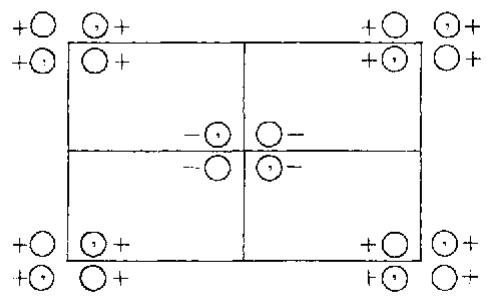
\includegraphics[width=0.72\textwidth]{fig3_17a_mu.jpg}
\caption*{\textbf{图 3.17(a)}\ 《国际表》（Henry and Lonsdale 1965）书影：$Pmmn$（$D_{2h}^{13}$）的第一种定向（原点在 $mmn$）。}
\end{figure}
\begin{figure}[H]
\centering
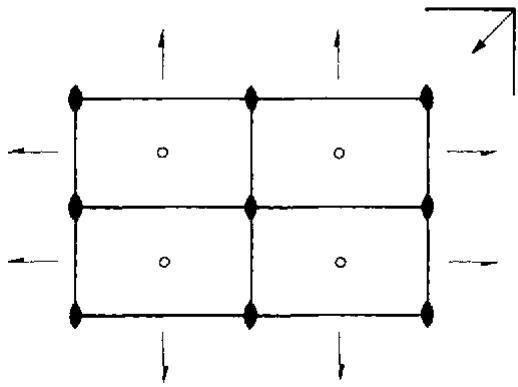
\includegraphics[width=0.72\textwidth]{fig3_17b_mu.jpg}
\caption*{\textbf{图 3.17(b)}\ 同上，第二种定向（原点在 $\bar{1}$）。}
\end{figure}

重要的是要弄清：若把描述晶体所用的坐标系原点移到晶胞中另一点，给定的 Seitz 空间群符号 $\{R_{1} \mid \mathbf{v}_{1}\}$ 的形式会受到什么影响。设 $\mathbf{r}_{1}$ 与 $\mathbf{r}_{1}'$ 是某个点在施加一个主动空间群对称操作前、后的位置；在第一组坐标轴 $O_{1}x_{1}y_{1}z_{1}$ 中该操作记为 $\{R_{1} \mid \mathbf{v}_{1}\}$。现在另取一组坐标轴 $O_{2}x_{2}y_{2}z_{2}$，其原点相对 $O_{1}x_{1}y_{1}z_{1}$ 的原点移动了矢量 $+\mathbf{t}_{0}$ 而轴不转动，见图 3.18。由该图可见
\begin{equation*}
\mathbf{r}_{1} = \mathbf{t}_{0} + \mathbf{r}_{2}
\tag{3.5.5}
\end{equation*}
及
\begin{equation*}
\mathbf{r}_{1}' = \mathbf{t}_{0} + \mathbf{r}_{2}',
\tag{3.5.6}
\end{equation*}
又由在 $O_{1}x_{1}y_{1}z_{1}$ 中使用的空间群符号 $\{R_{1} \mid \mathbf{v}_{1}\}$ 的定义，
\begin{equation*}
\mathbf{r}_{1}' = R_{1}\mathbf{r}_{1} + \mathbf{v}_{1}.
\tag{3.5.4}
\end{equation*}
若这一空间群操作在坐标系 $O_{2}x_{2}y_{2}z_{2}$ 中记为 $\{R_{2} \mid \mathbf{v}_{2}\}$，则 $\mathbf{r}_{2}'$ 与 $\mathbf{r}_{2}$ 满足
\begin{equation*}
\mathbf{r}_{2}' = R_{2}\mathbf{r}_{2} + \mathbf{v}_{2}
\tag{3.5.7}
\end{equation*}
于是可以用这些方程把 $\{R_{2} \mid \mathbf{v}_{2}\}$ 用 $\{R_{1} \mid \mathbf{v}_{1}\}$ 表示出来。由式 (3.5.7)，
\begin{align*}
R_{2}\mathbf{r}_{2} + \mathbf{v}_{2} &= \mathbf{r}_{2}' = \mathbf{r}_{1}' - \mathbf{t}_{0} \quad\text{（由 (3.5.6)）}\\
&= R_{1}\mathbf{r}_{1} + \mathbf{v}_{1} - \mathbf{t}_{0} \quad\text{（由 (3.5.4)）}\\
&= R_{1}(\mathbf{t}_{0} + \mathbf{r}_{2}) + \mathbf{v}_{1} - \mathbf{t}_{0} \quad\text{（由 (3.5.5)）}\\
&= R_{1}\mathbf{r}_{2} + \mathbf{v}_{1} + R_{1}\mathbf{t}_{0} - \mathbf{t}_{0},
\end{align*}
即
\begin{equation*}
R_{2}\mathbf{r}_{2} + \mathbf{v}_{2} = R_{1}\mathbf{r}_{2} + \mathbf{v}_{1} + R_{1}\mathbf{t}_{0} - \mathbf{t}_{0}.
\tag{3.5.8}
\end{equation*}
比较式 (3.5.8) 两边可见，把原点移动 $+\mathbf{t}_{0}$ 对空间群符号 $\{R_{1} \mid \mathbf{v}_{1}\}$ 的效果是产生 $\{R_{2} \mid \mathbf{v}_{2}\}$，其中
\begin{equation*}
R_{2} = R_{1}
\tag{3.5.9}
\end{equation*}
及
\begin{equation*}
\mathbf{v}_{2} = \mathbf{v}_{1} + R_{1}\mathbf{t}_{0} - \mathbf{t}_{0}.
\tag{3.5.10}
\end{equation*}
也就是说，移动原点 $+\mathbf{t}_{0}$ 对空间群符号 $\{R_{1} \mid \mathbf{v}_{1}\}$ 的效果是产生
\begin{equation*}
\{R_{2} \mid \mathbf{v}_{2}\} = \{R_{1} \mid \mathbf{v}_{1} + R_{1}\mathbf{t}_{0} - \mathbf{t}_{0}\}.
\tag{3.5.11}
\end{equation*}

\begin{figure}[H]
\centering
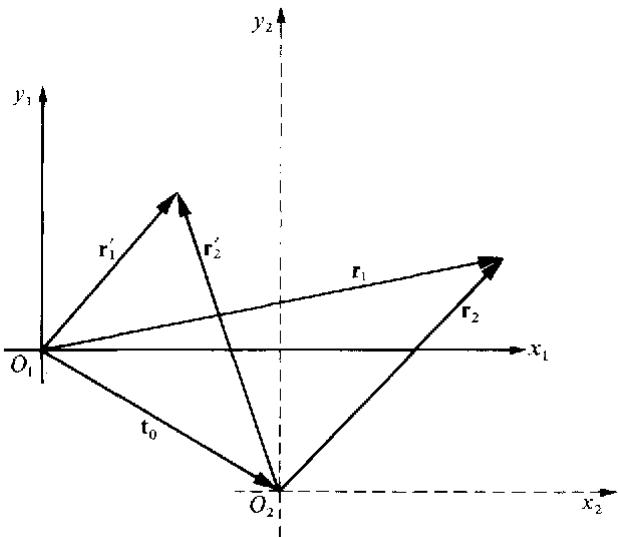
\includegraphics[width=0.55\textwidth]{fig3_18_mu.jpg}
\caption*{\textbf{图 3.18}\ 通过一个平移改变原点。}
\end{figure}

我们仍以空间群 $Pmmn$（$D_{2h}^{13}$）为例说明移动原点对空间群符号的影响。《国际表》对该空间群给出了两种不同的定向，见图 3.17。上面我们已用第一种定向（图 3.17(a)）写出了空间群元素。在第二种定向（图 3.17(b)）中，原点移动了（沿 $x$ 轴重复距离的 $-\frac{1}{4}$）加（沿 $y$ 轴重复距离的 $-\frac{1}{4}$），即由表 3.1，
\begin{equation*}
\mathbf{t}_{0} = \frac{1}{4}\mathbf{t}_{1} - \frac{1}{4}\mathbf{t}_{2}.
\tag{3.5.12}
\end{equation*}
于是利用式 (3.5.9) 与 (3.5.10)，可以把先前得到的空间群元素转换到第二组轴上。例如 $\{C_{2z} \mid 000\}$ 被 $\{R_{2} \mid \mathbf{v}_{2}\}$ 取代，其中由式 (3.5.9)，$R_{2} = C_{2z}$，而
\begin{align*}
\mathbf{v}_{2} &= \mathbf{v}_{1} + R_{1}\mathbf{t}_{0} - \mathbf{t}_{0}\\
&= \mathbf{0} + C_{2z}\left(\tfrac{1}{4}\mathbf{t}_{1} - \tfrac{1}{4}\mathbf{t}_{2}\right) - \left(\tfrac{1}{4}\mathbf{t}_{1} - \tfrac{1}{4}\mathbf{t}_{2}\right)\\
&= \left(-\tfrac{1}{4}\mathbf{t}_{1} + \tfrac{1}{4}\mathbf{t}_{2}\right) - \left(\tfrac{1}{4}\mathbf{t}_{1} - \tfrac{1}{4}\mathbf{t}_{2}\right)\quad\text{（由表 3.2）}\\
&= -\tfrac{1}{2}\mathbf{t}_{1} + \tfrac{1}{2}\mathbf{t}_{2},
\tag{3.5.13}
\end{align*}
故新坐标系中的元素为 $\{C_{2z} \mid \bar{\frac{1}{2}}\bar{\frac{1}{2}}0\}$，可以加上 $\mathbf{t}_{1}$ 得到以新原点为基准的空间群元素 $\{C_{2z} \mid \frac{1}{2}\frac{1}{2}0\}$。这与图 3.17(b) 所示的等价位置一致：$\{C_{2z} \mid \frac{1}{2}\frac{1}{2}0\}$ 作用在 $(x, y, z)$ 上产生 $(\frac{1}{2}-x, \frac{1}{2}-y, z)$，这正是图 3.17(b) 给出的八个一般等价位置之一。对同样的 $\mathbf{t}_{0} = \frac{1}{4}\mathbf{t}_{1} - \frac{1}{4}\mathbf{t}_{2}$ 反复使用式 (3.5.9) 与 (3.5.10)，得到以新原点为基准的空间群 $Pmmn$（$D_{2h}^{13}$）的全部元素：
\begin{center}
$\{E \mid 000\}$，$\{C_{2z} \mid \frac{1}{2}\frac{1}{2}0\}$，$\{\sigma_{x} \mid 0\frac{1}{2}0\}$，$\{\sigma_{y} \mid \frac{1}{2}00\}$，\\[0.5ex]
$\{I \mid 000\}$，$\{\sigma_{z} \mid \frac{1}{2}\frac{1}{2}0\}$，$\{C_{2x} \mid 0\frac{1}{2}0\}$，$\{C_{2y} \mid \frac{1}{2}00\}$。
\end{center}
在这个清单里，我们在某些情况下加上或减去了正交初基布拉维格子平移群的矢量，以简化空间群元素的形式。

230 个空间群中每一个的生成元都列于表 3.7。在前三列中我们用国际符号和 Schönflies 符号标识空间群，第 4 列给出足以确定空间群 $\mathbf{G}$ 全部元素的 Seitz 空间群符号，其中 $\{R \mid pqr\}$ 表示 $\{R \mid p\mathbf{t}_{1} + q\mathbf{t}_{2} + r\mathbf{t}_{3}\}$，$\mathbf{t}_{1}$、$\mathbf{t}_{2}$、$\mathbf{t}_{3}$ 按表 3.1 的定义。这些操作一如既往地用 1.5 节解释的 Seitz 记号表示（见式 (1.5.2) 与 (1.5.3)）。

\begin{figure}[H]
\centering
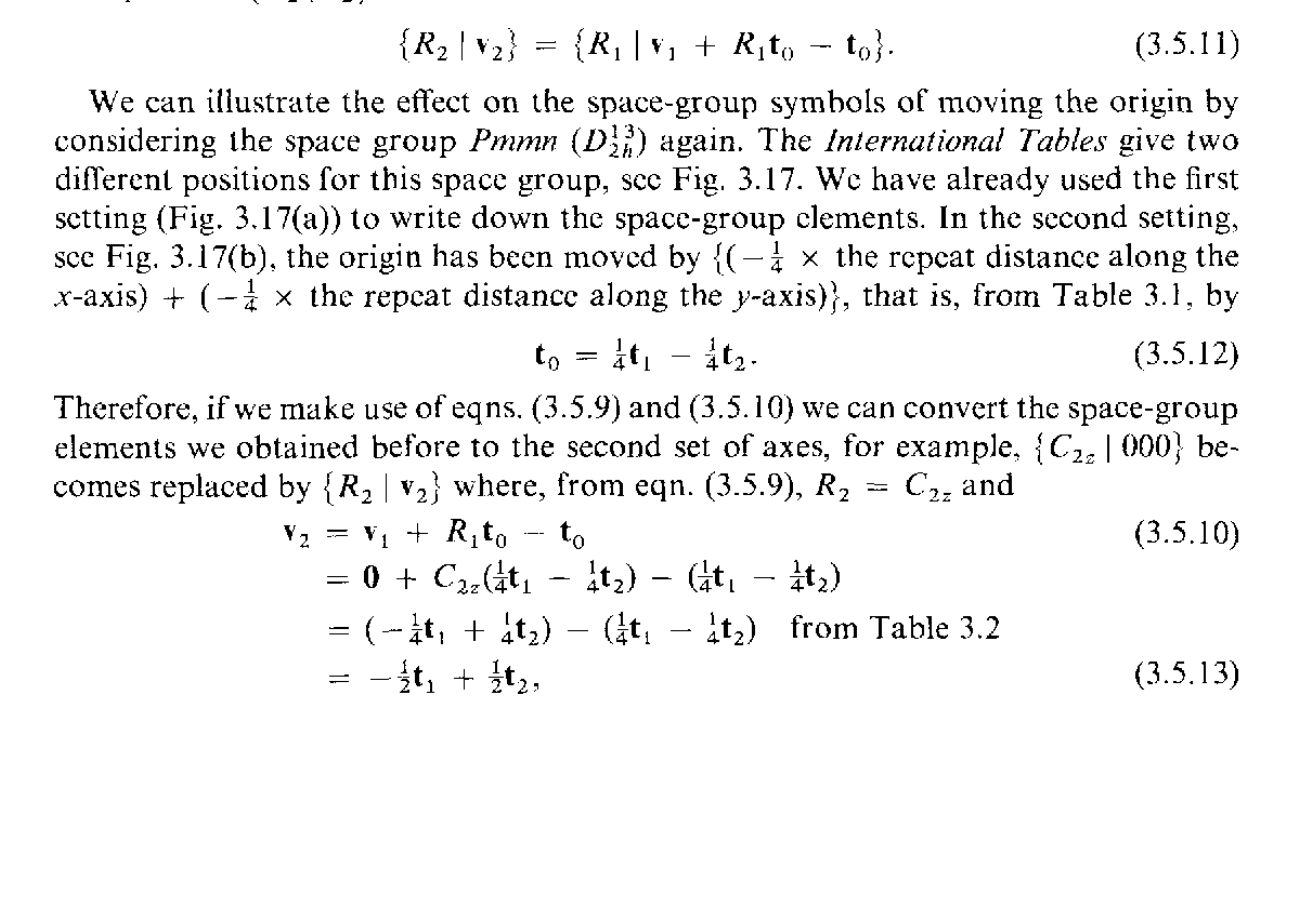
\includegraphics[width=0.92\textwidth]{c3_t37_p1.png}
\caption*{\textbf{表 3.7}\ 230 个空间群（原书第 126 页起扫描；第 1 页）。}
\end{figure}
\begin{figure}[H]
\centering
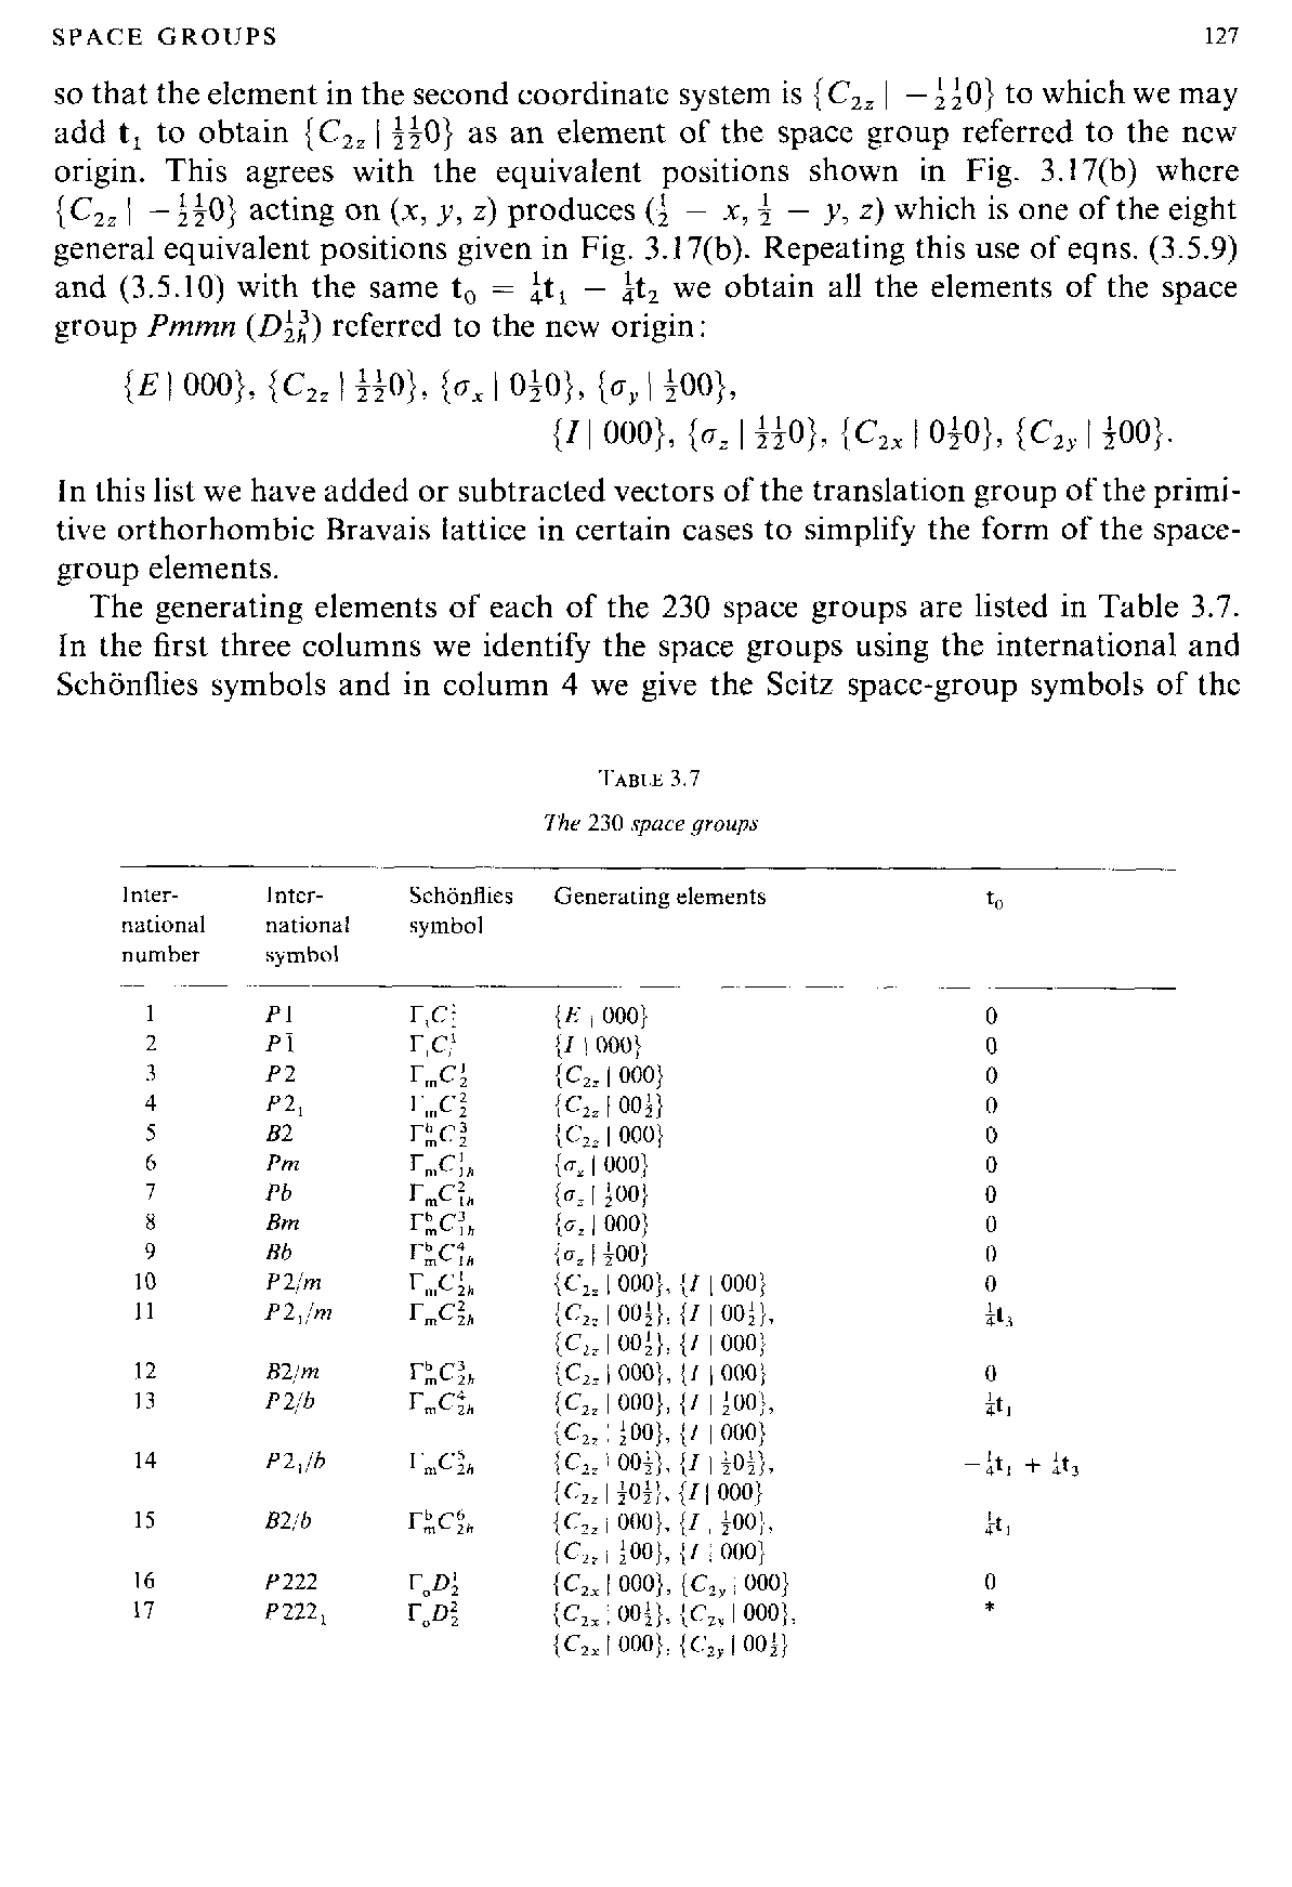
\includegraphics[width=0.92\textwidth]{c3_t37_p2.png}
\caption*{\textbf{表 3.7}（第 2 页）。}
\end{figure}
\begin{figure}[H]
\centering
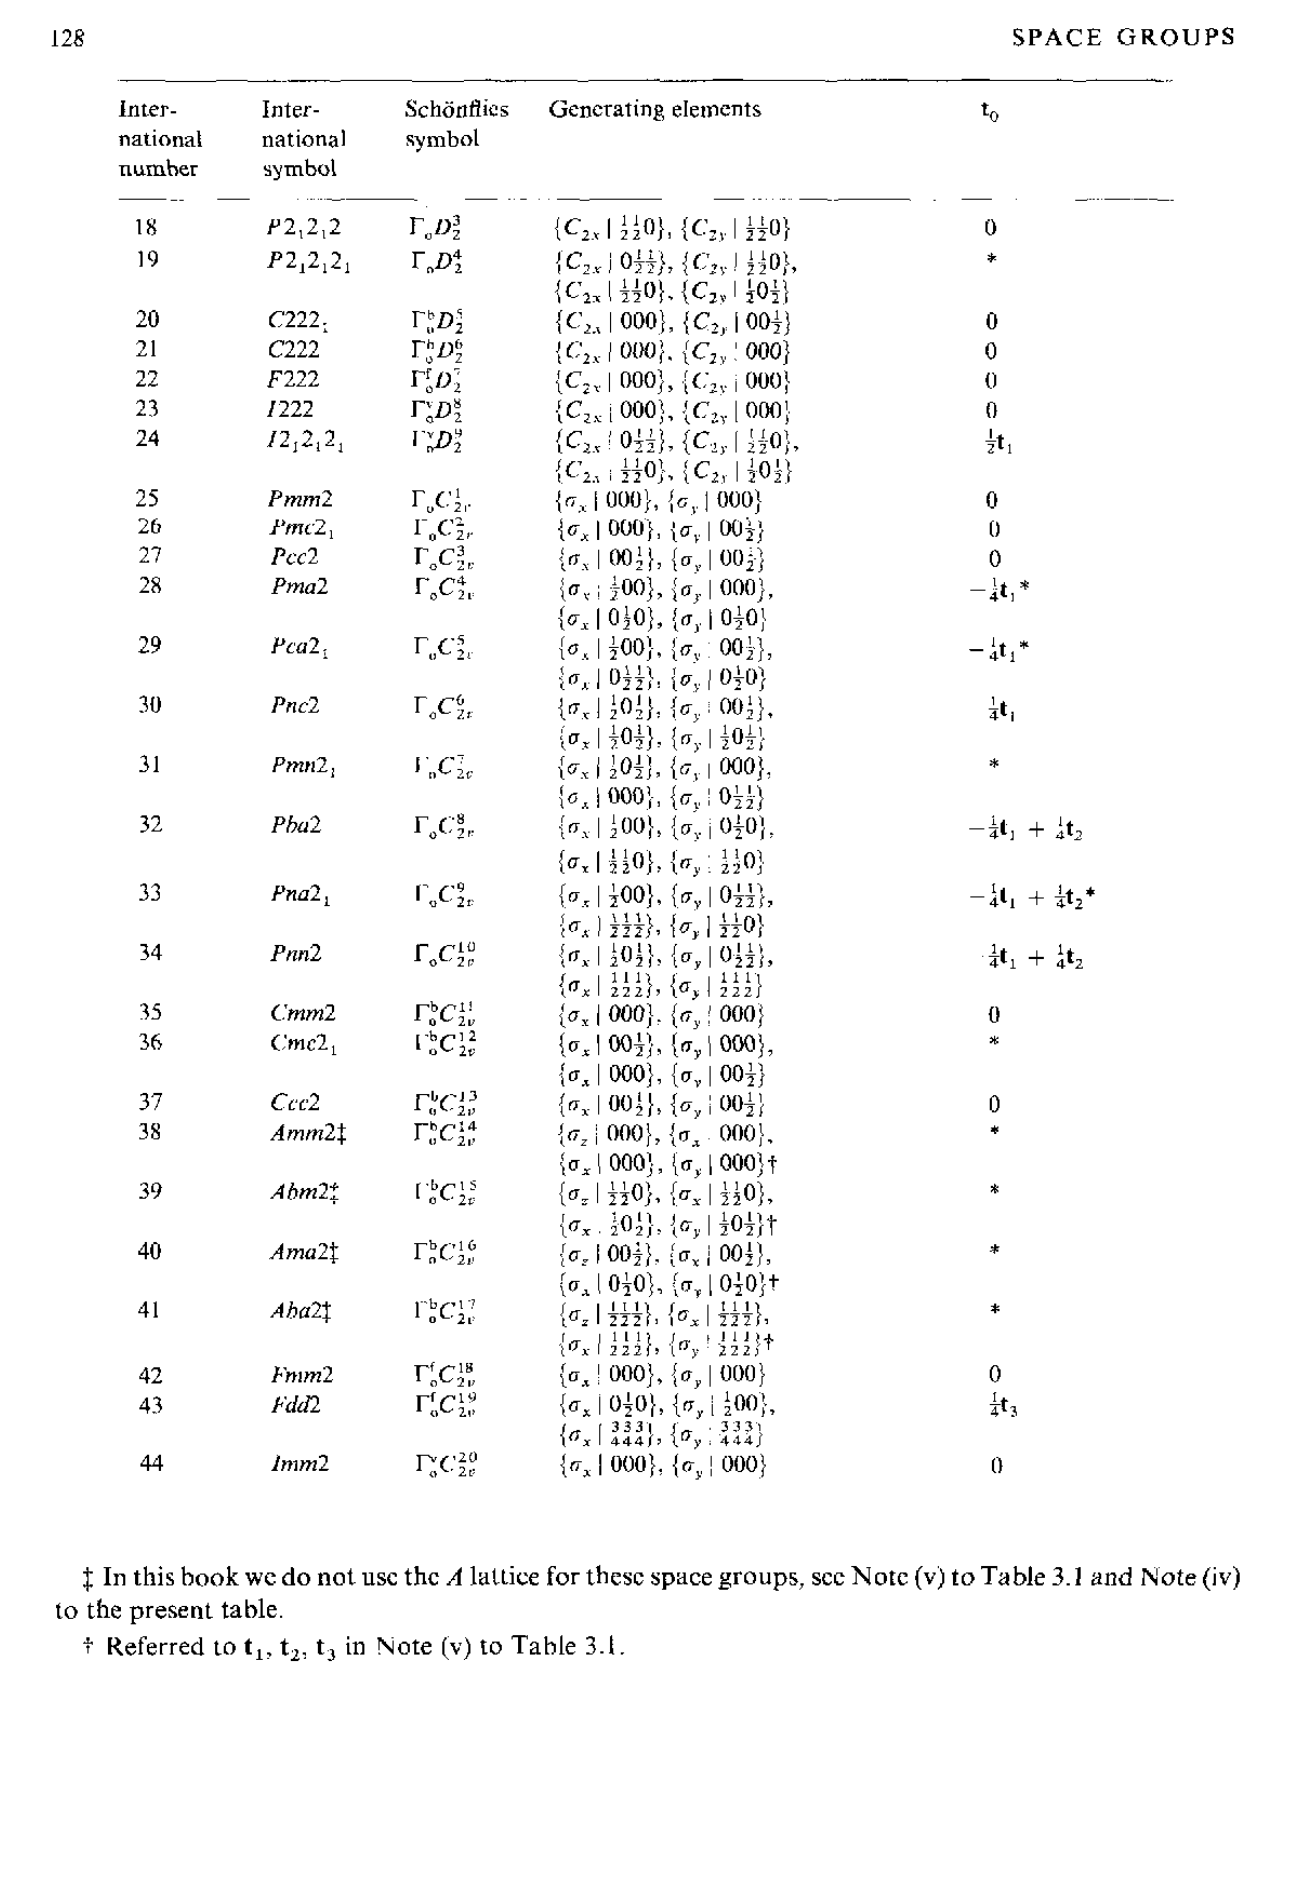
\includegraphics[width=0.92\textwidth]{c3_t37_p3.png}
\caption*{\textbf{表 3.7}（第 3 页）。}
\end{figure}
\begin{figure}[H]
\centering
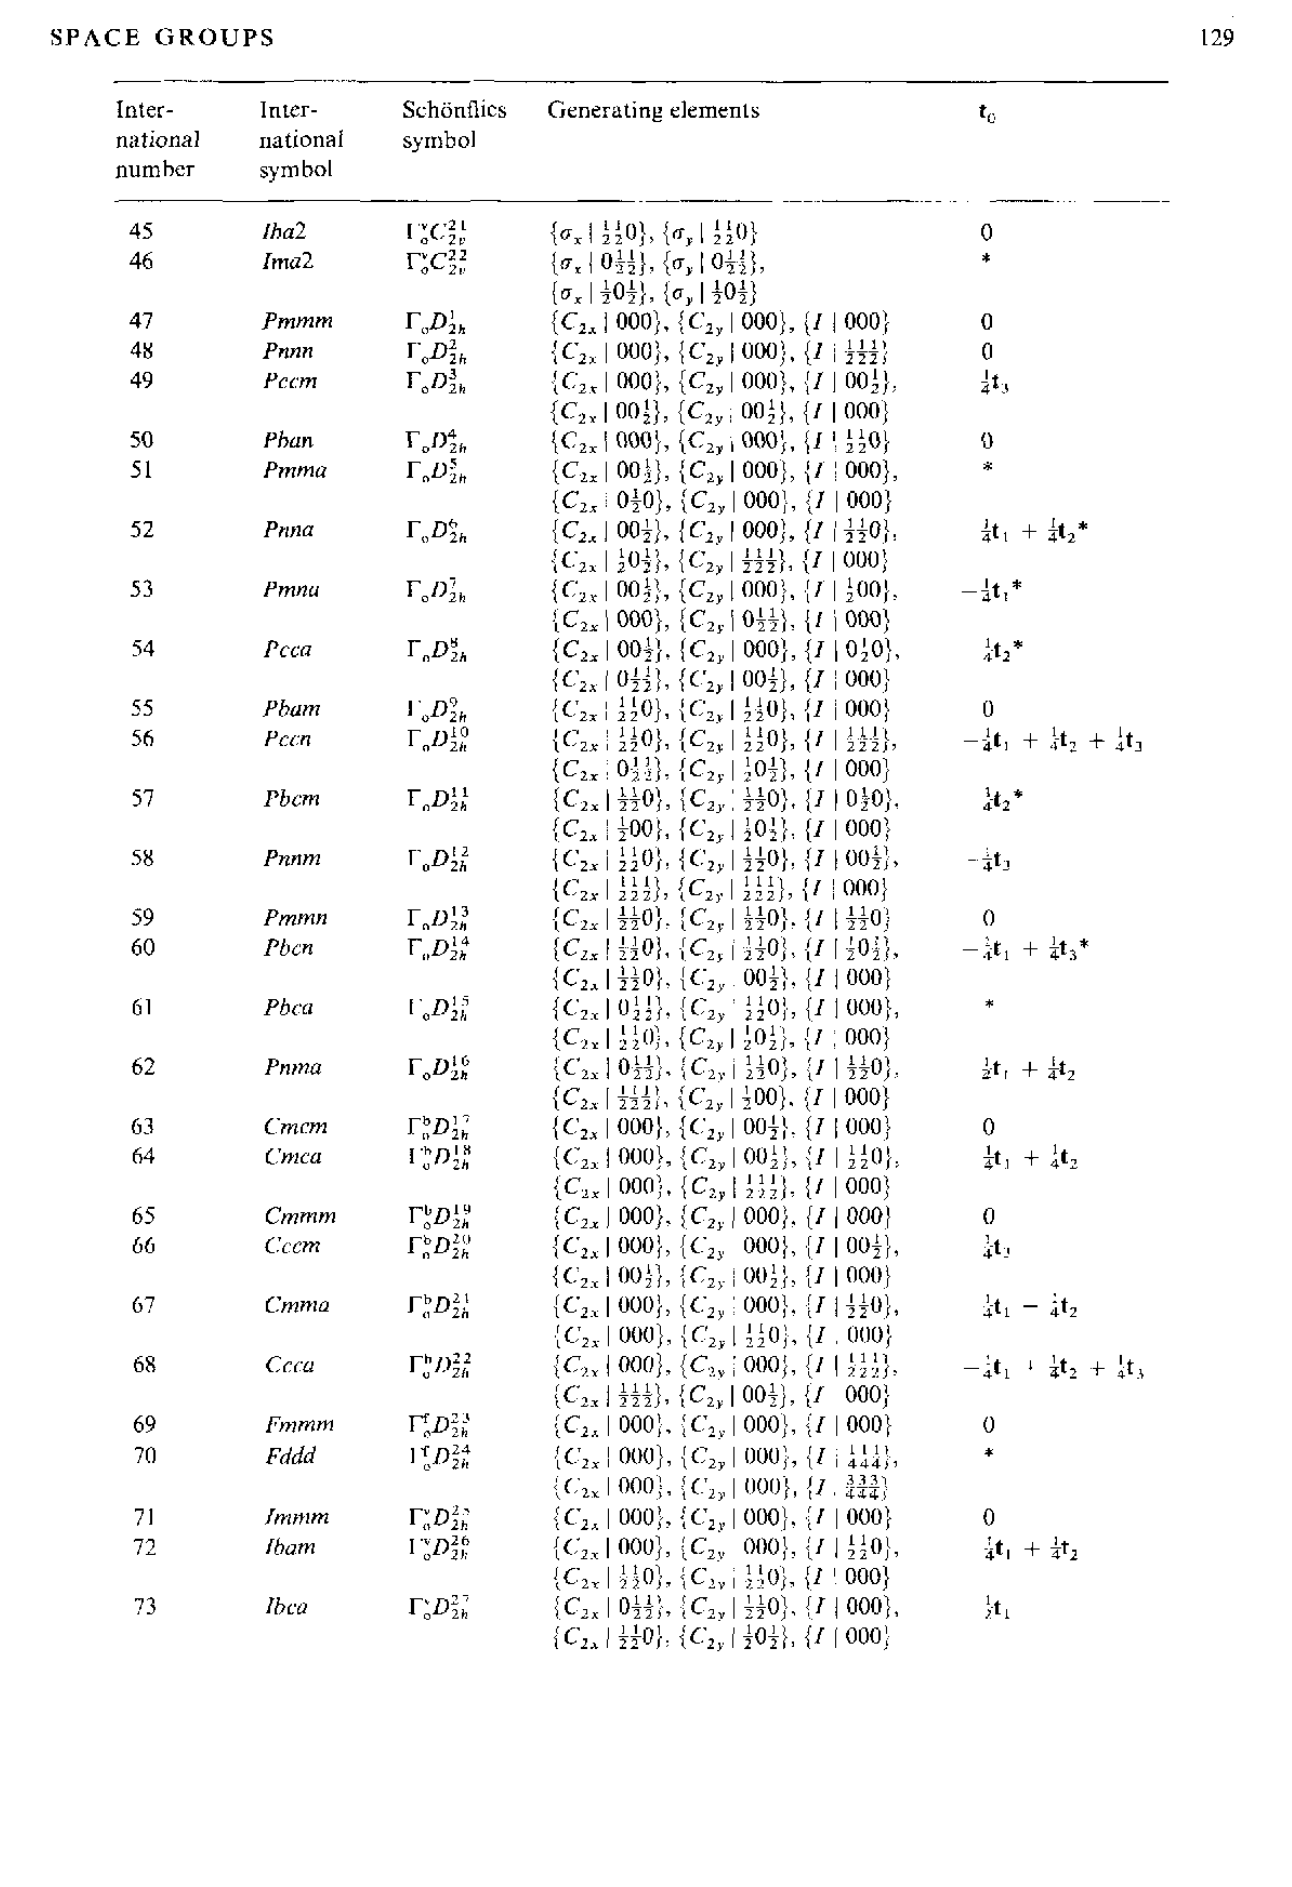
\includegraphics[width=0.92\textwidth]{c3_t37_p4.png}
\caption*{\textbf{表 3.7}（第 4 页）。}
\end{figure}
\begin{figure}[H]
\centering
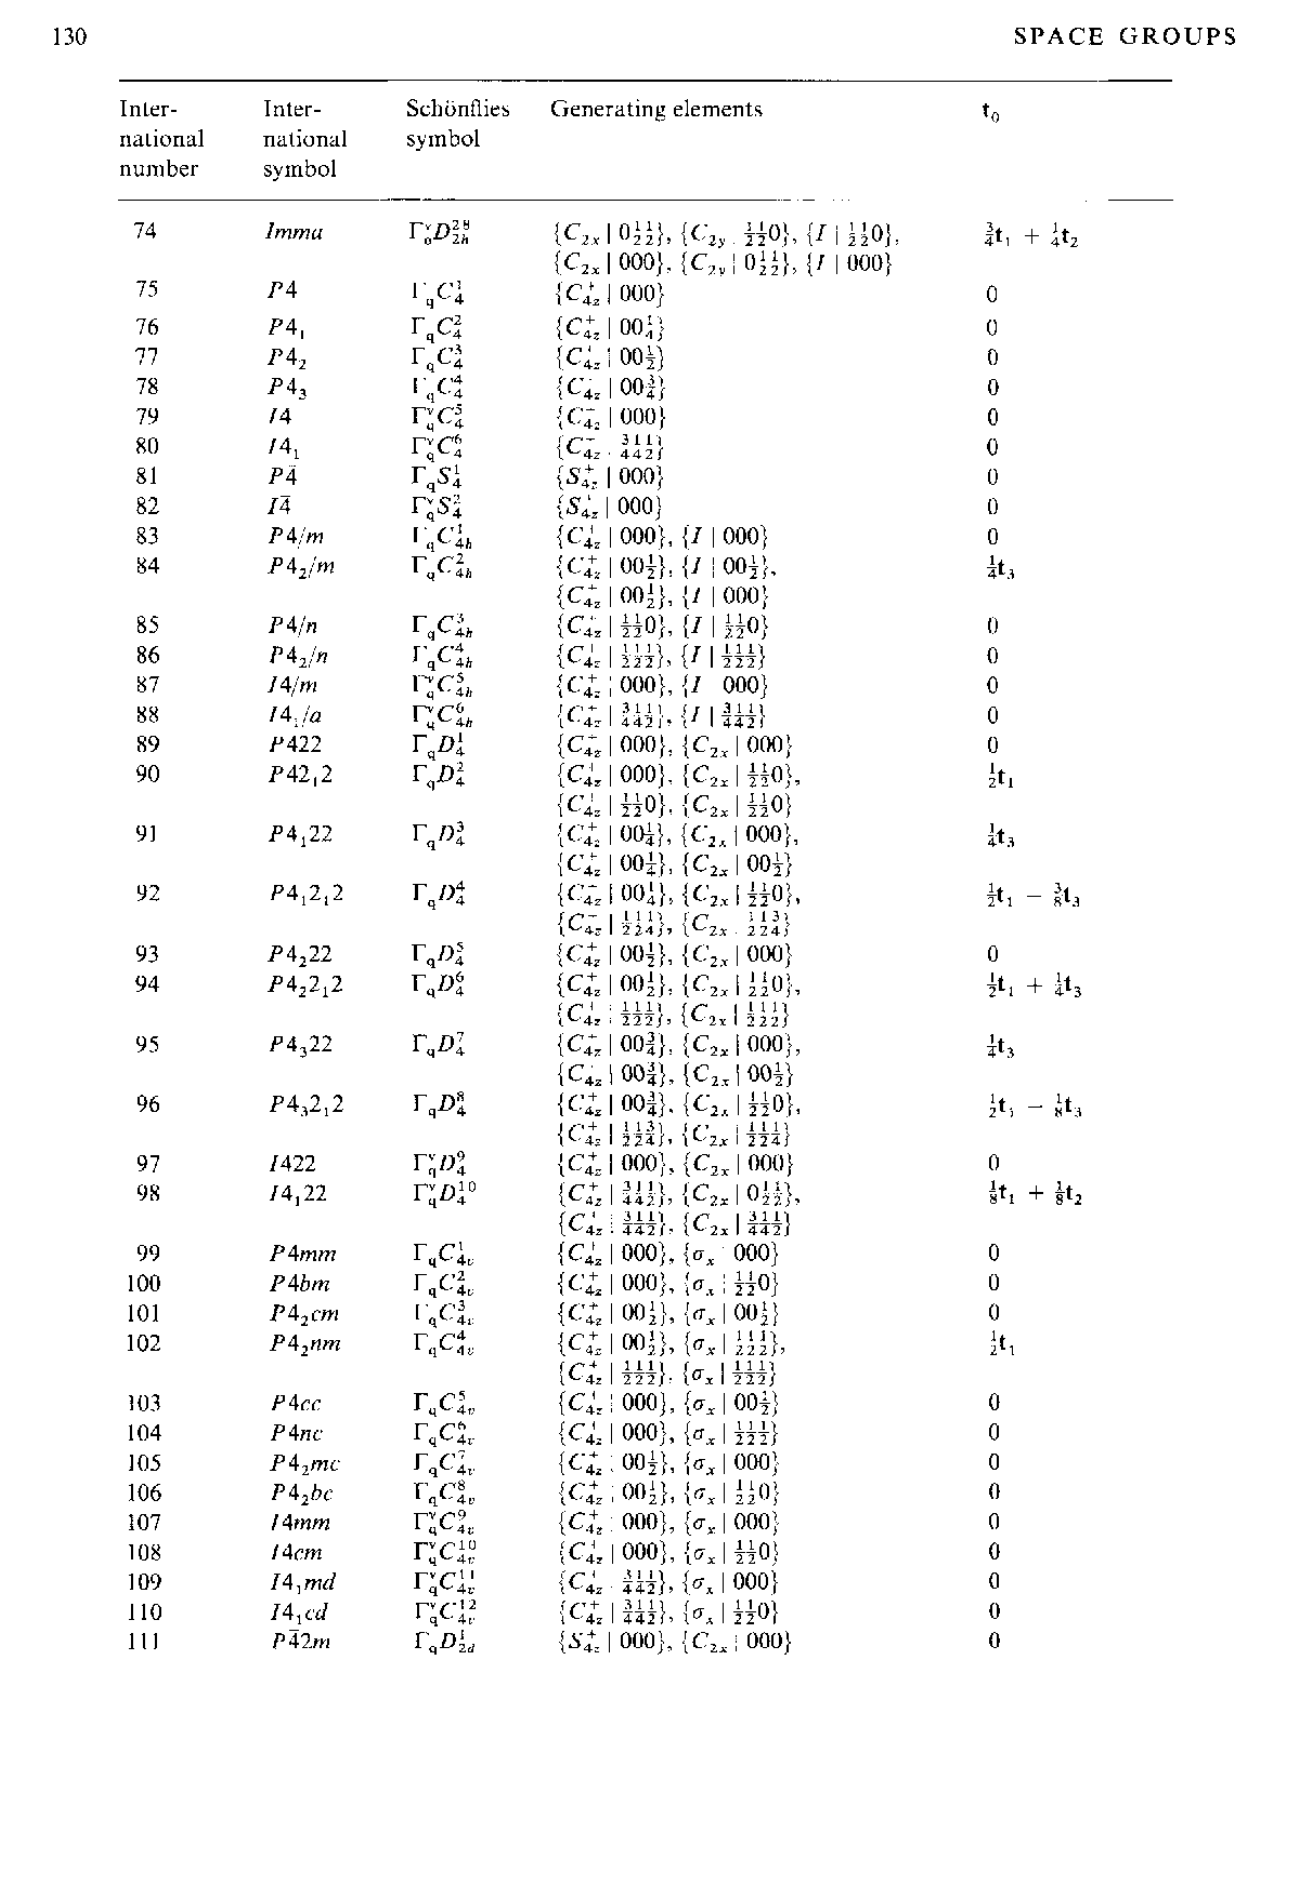
\includegraphics[width=0.92\textwidth]{c3_t37_p5.png}
\caption*{\textbf{表 3.7}（第 5 页）。}
\end{figure}
\begin{figure}[H]
\centering
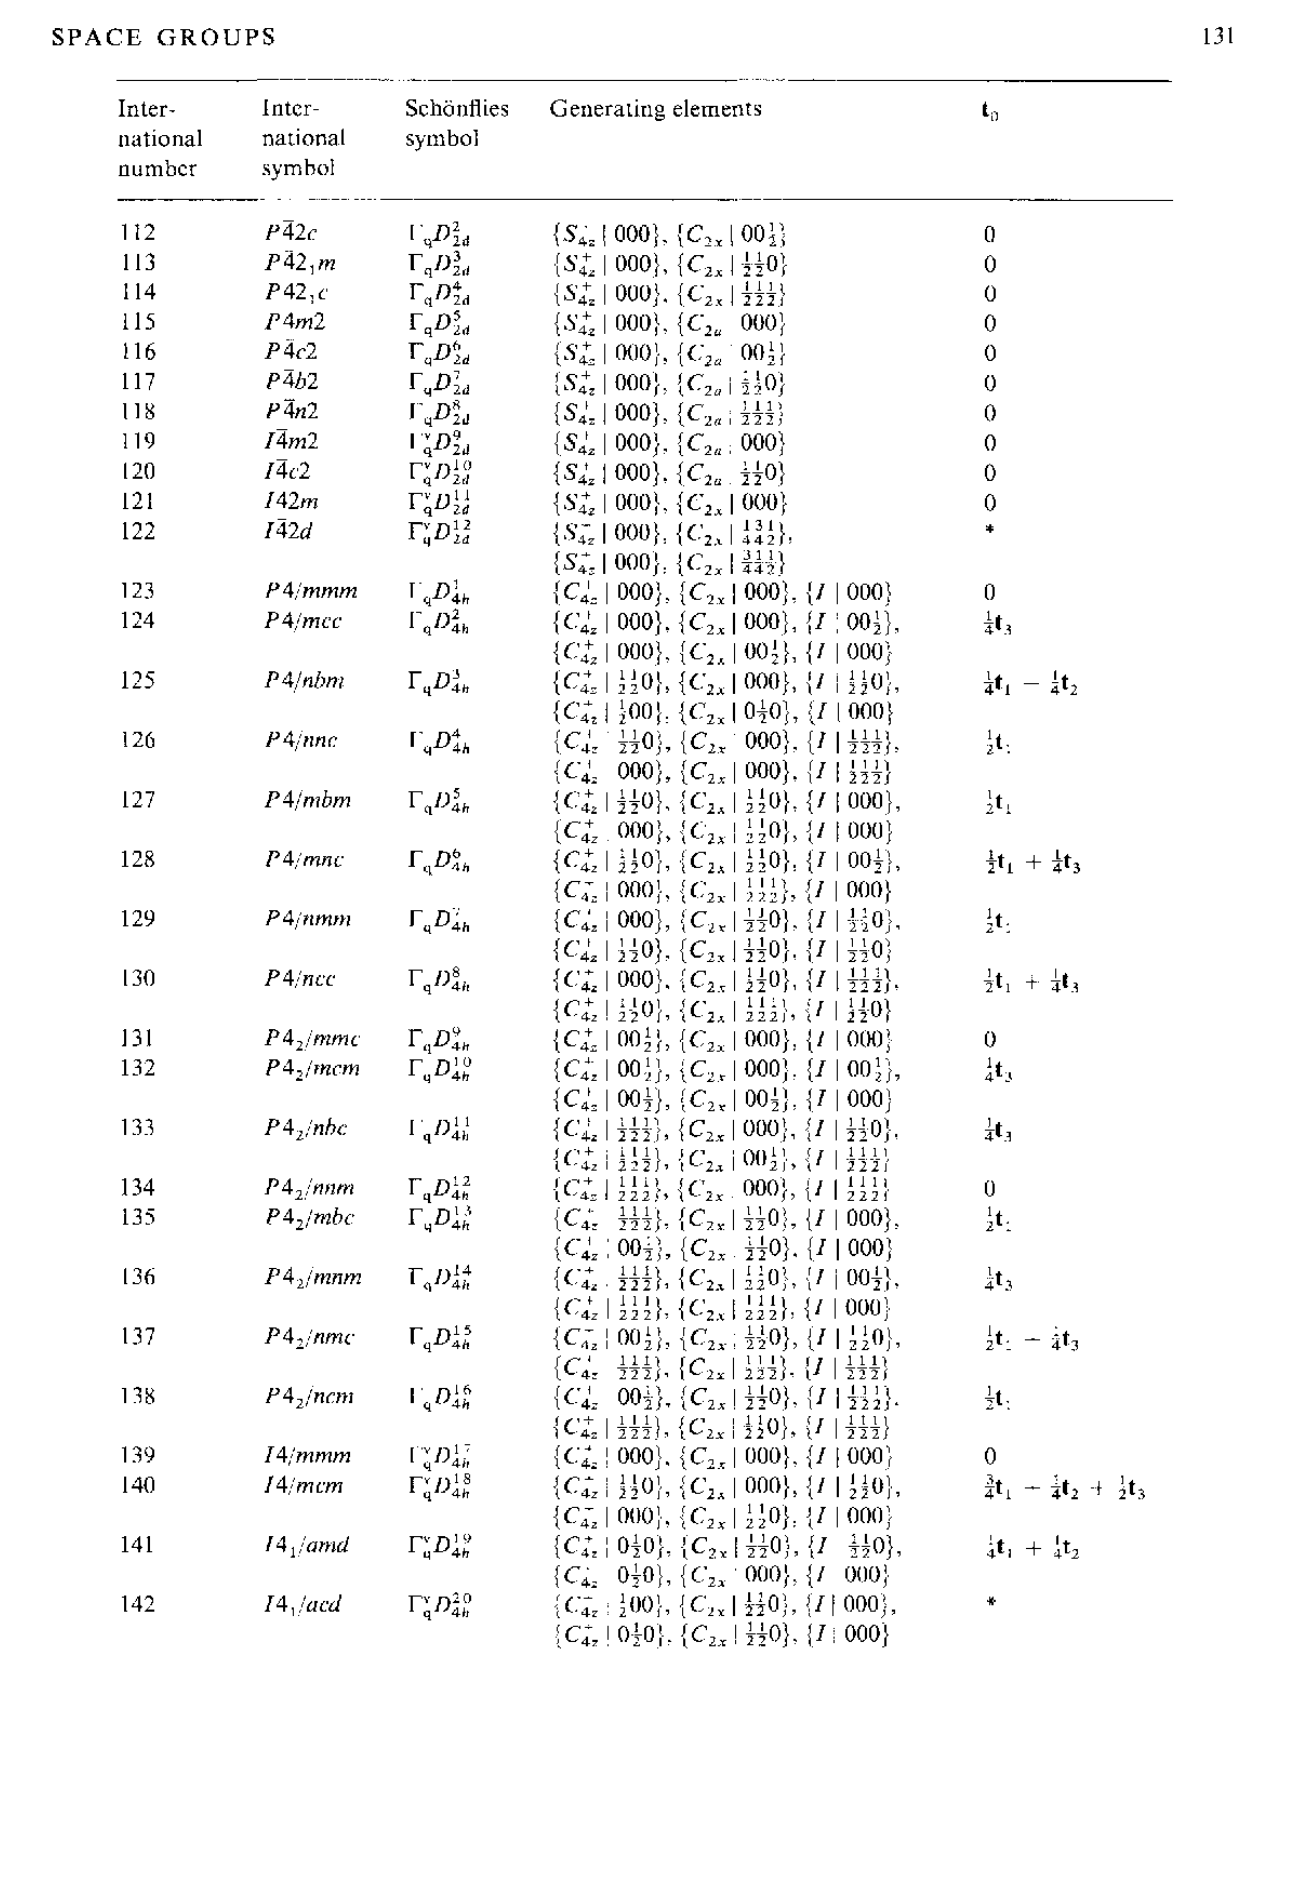
\includegraphics[width=0.92\textwidth]{c3_t37_p6.png}
\caption*{\textbf{表 3.7}（第 6 页）。}
\end{figure}
\begin{figure}[H]
\centering
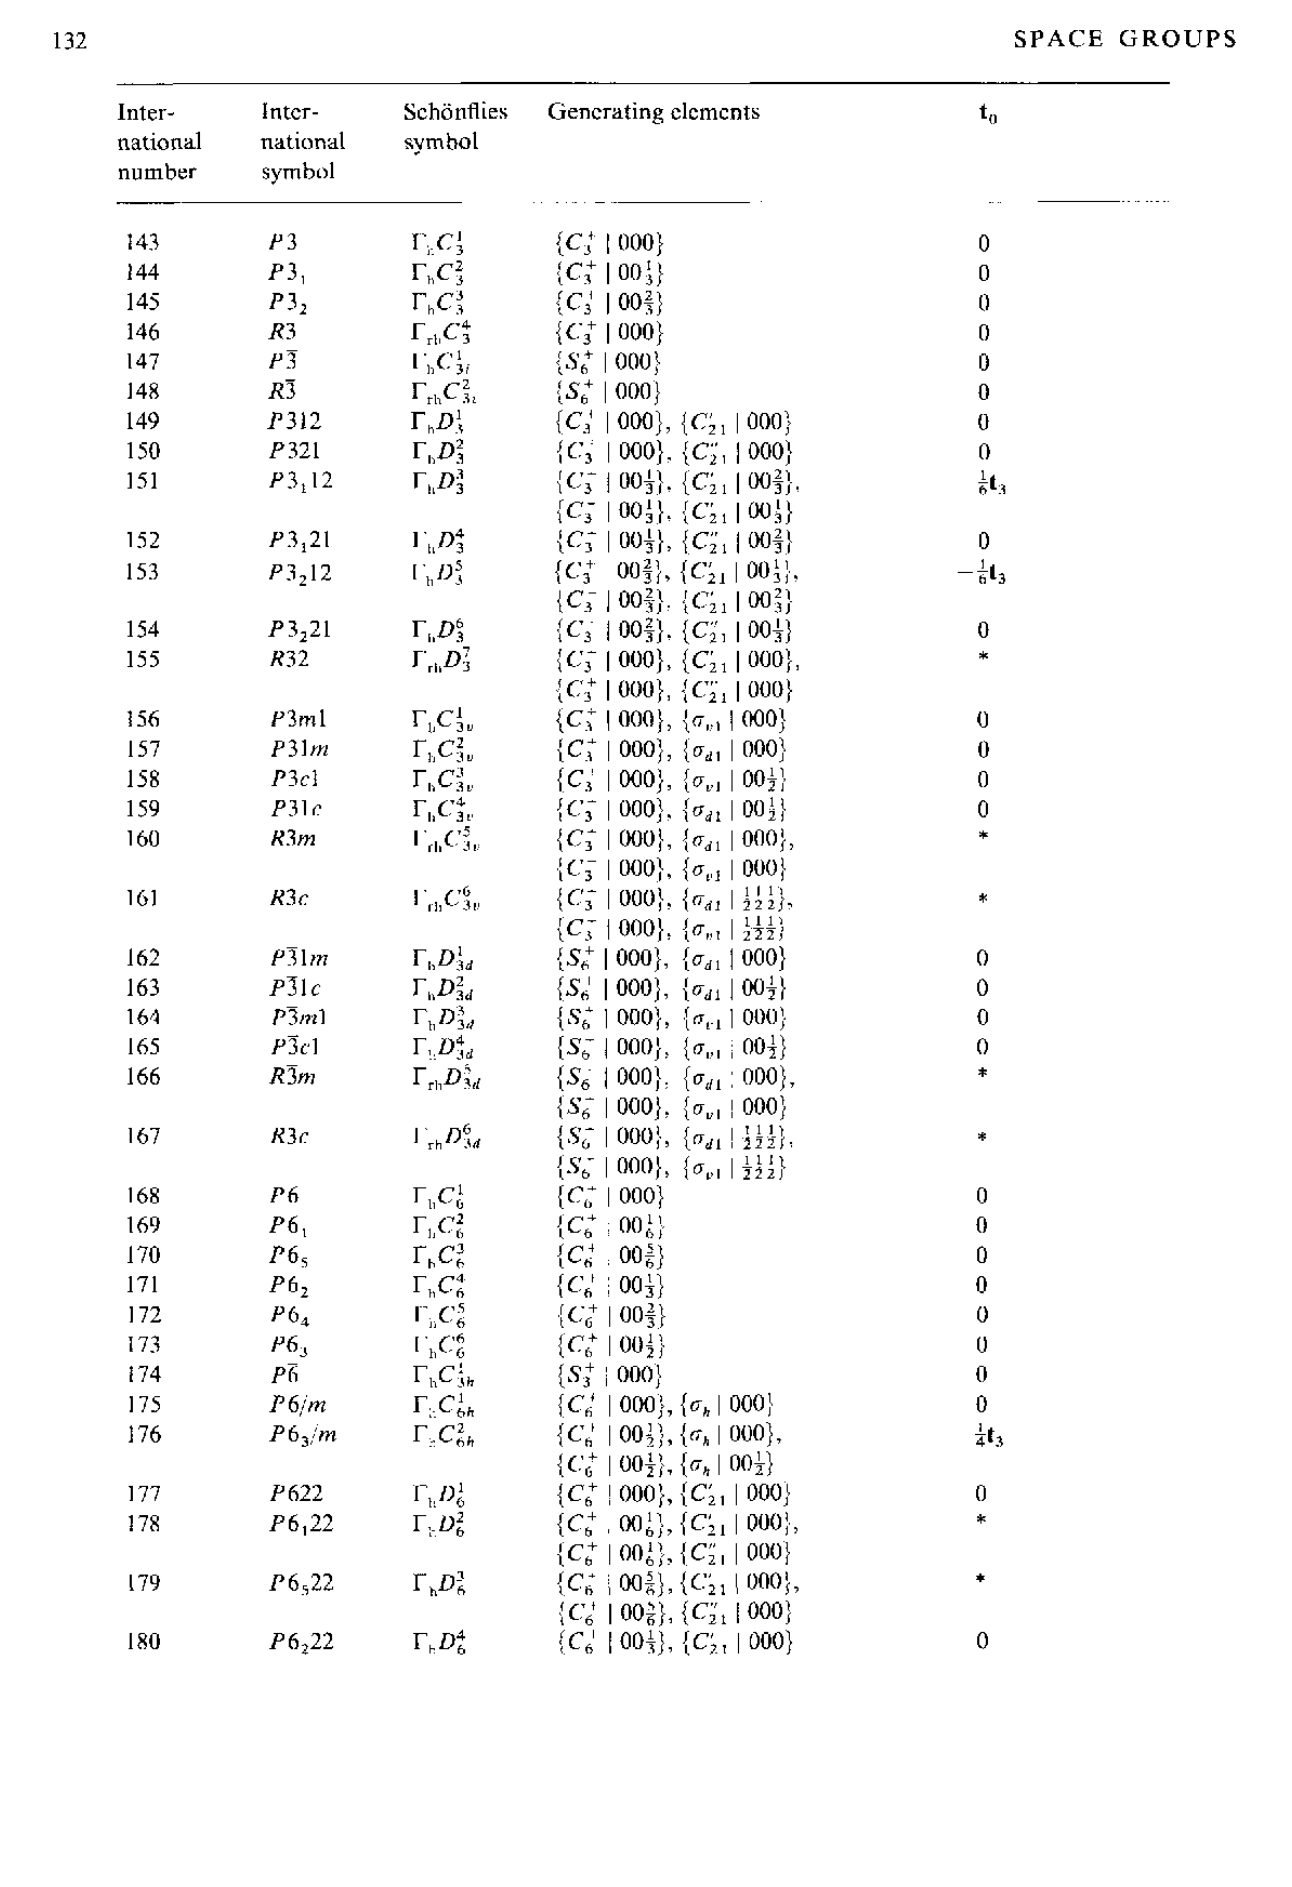
\includegraphics[width=0.92\textwidth]{c3_t37_p7.png}
\caption*{\textbf{表 3.7}（第 7 页）。}
\end{figure}
\begin{figure}[H]
\centering
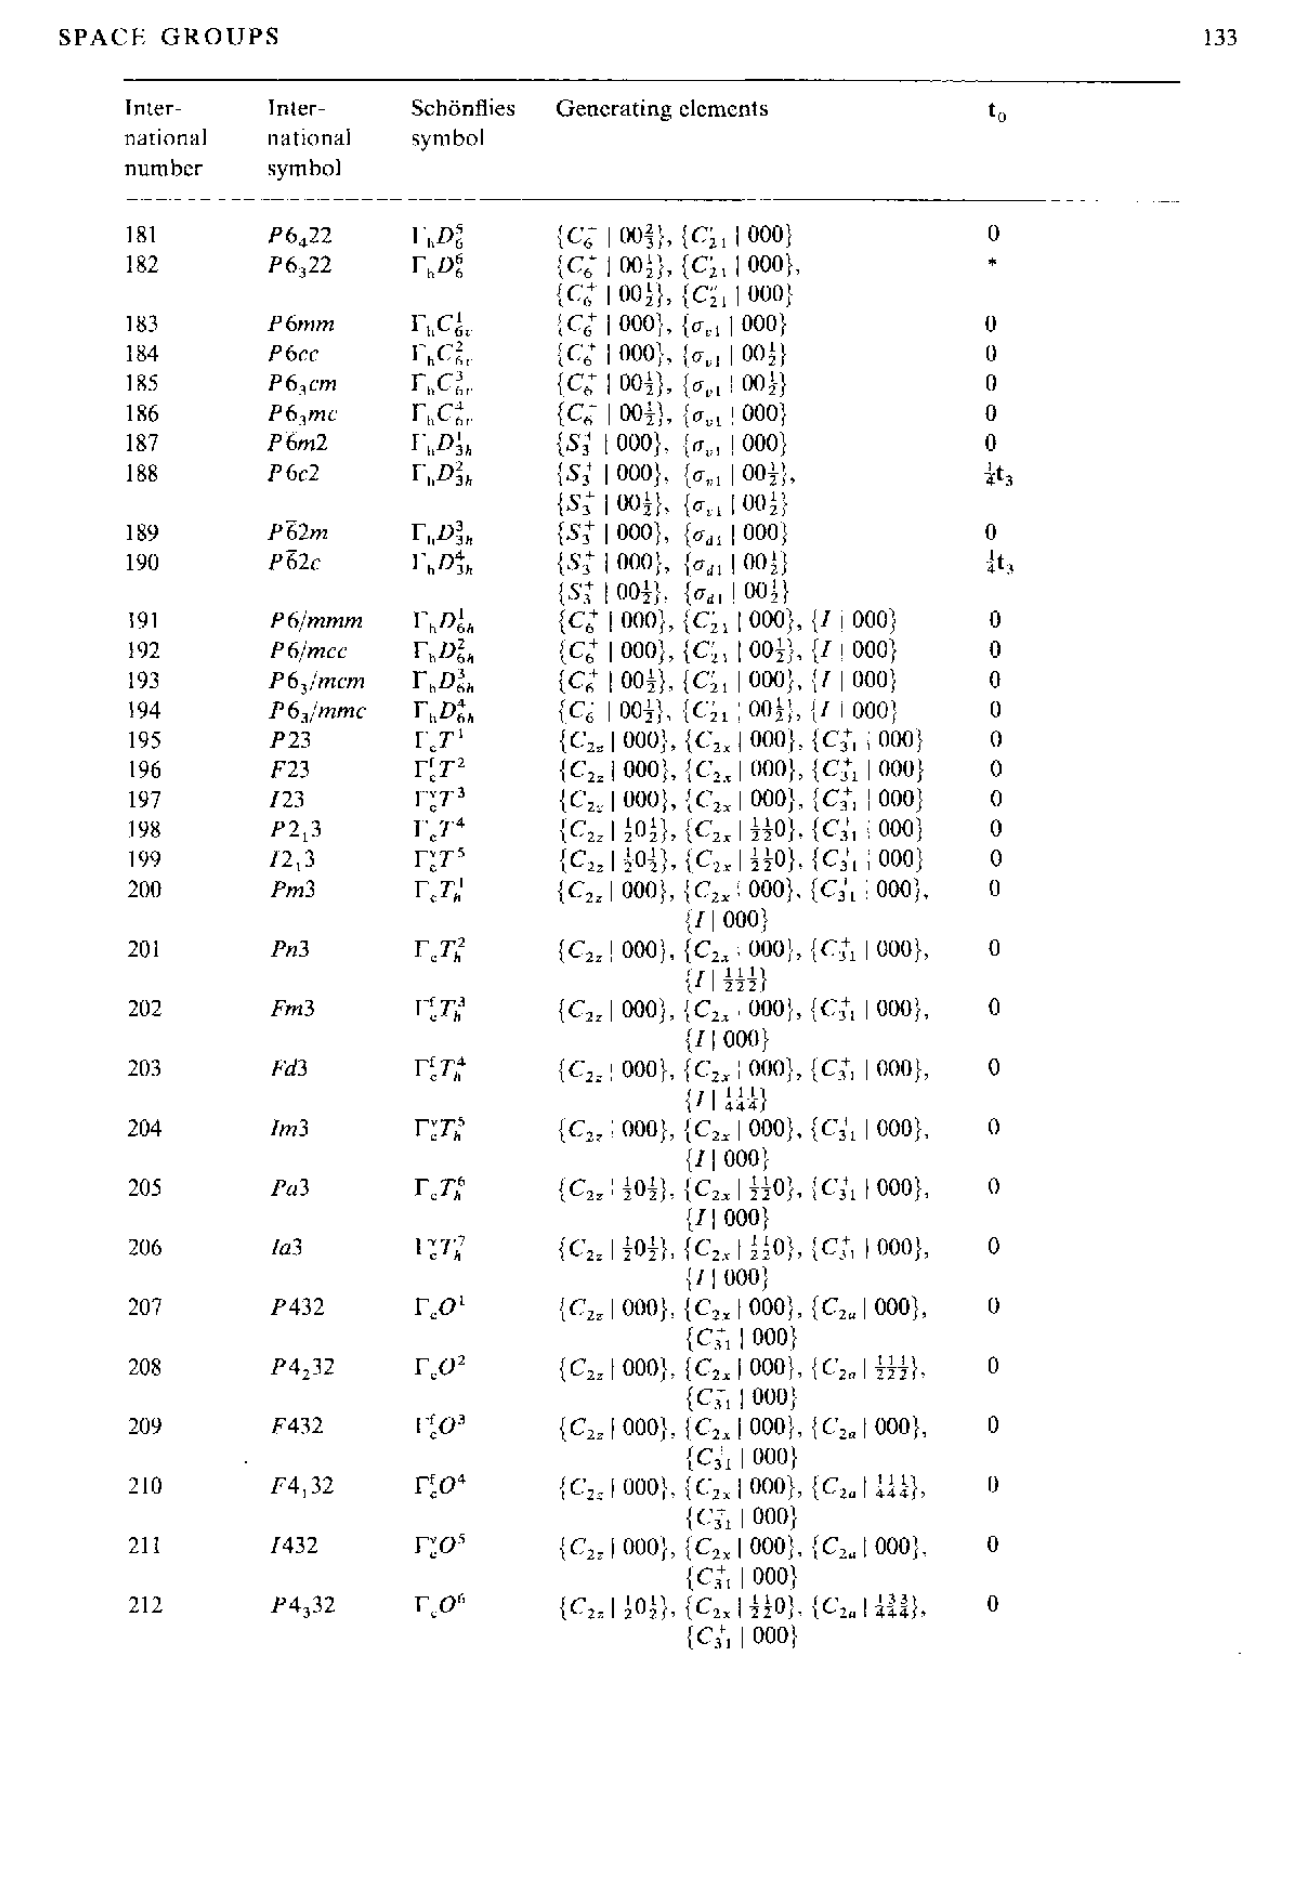
\includegraphics[width=0.92\textwidth]{c3_t37_p8.png}
\caption*{\textbf{表 3.7}（第 8 页，页末起为表的注）。}
\end{figure}
\begin{figure}[H]
\centering
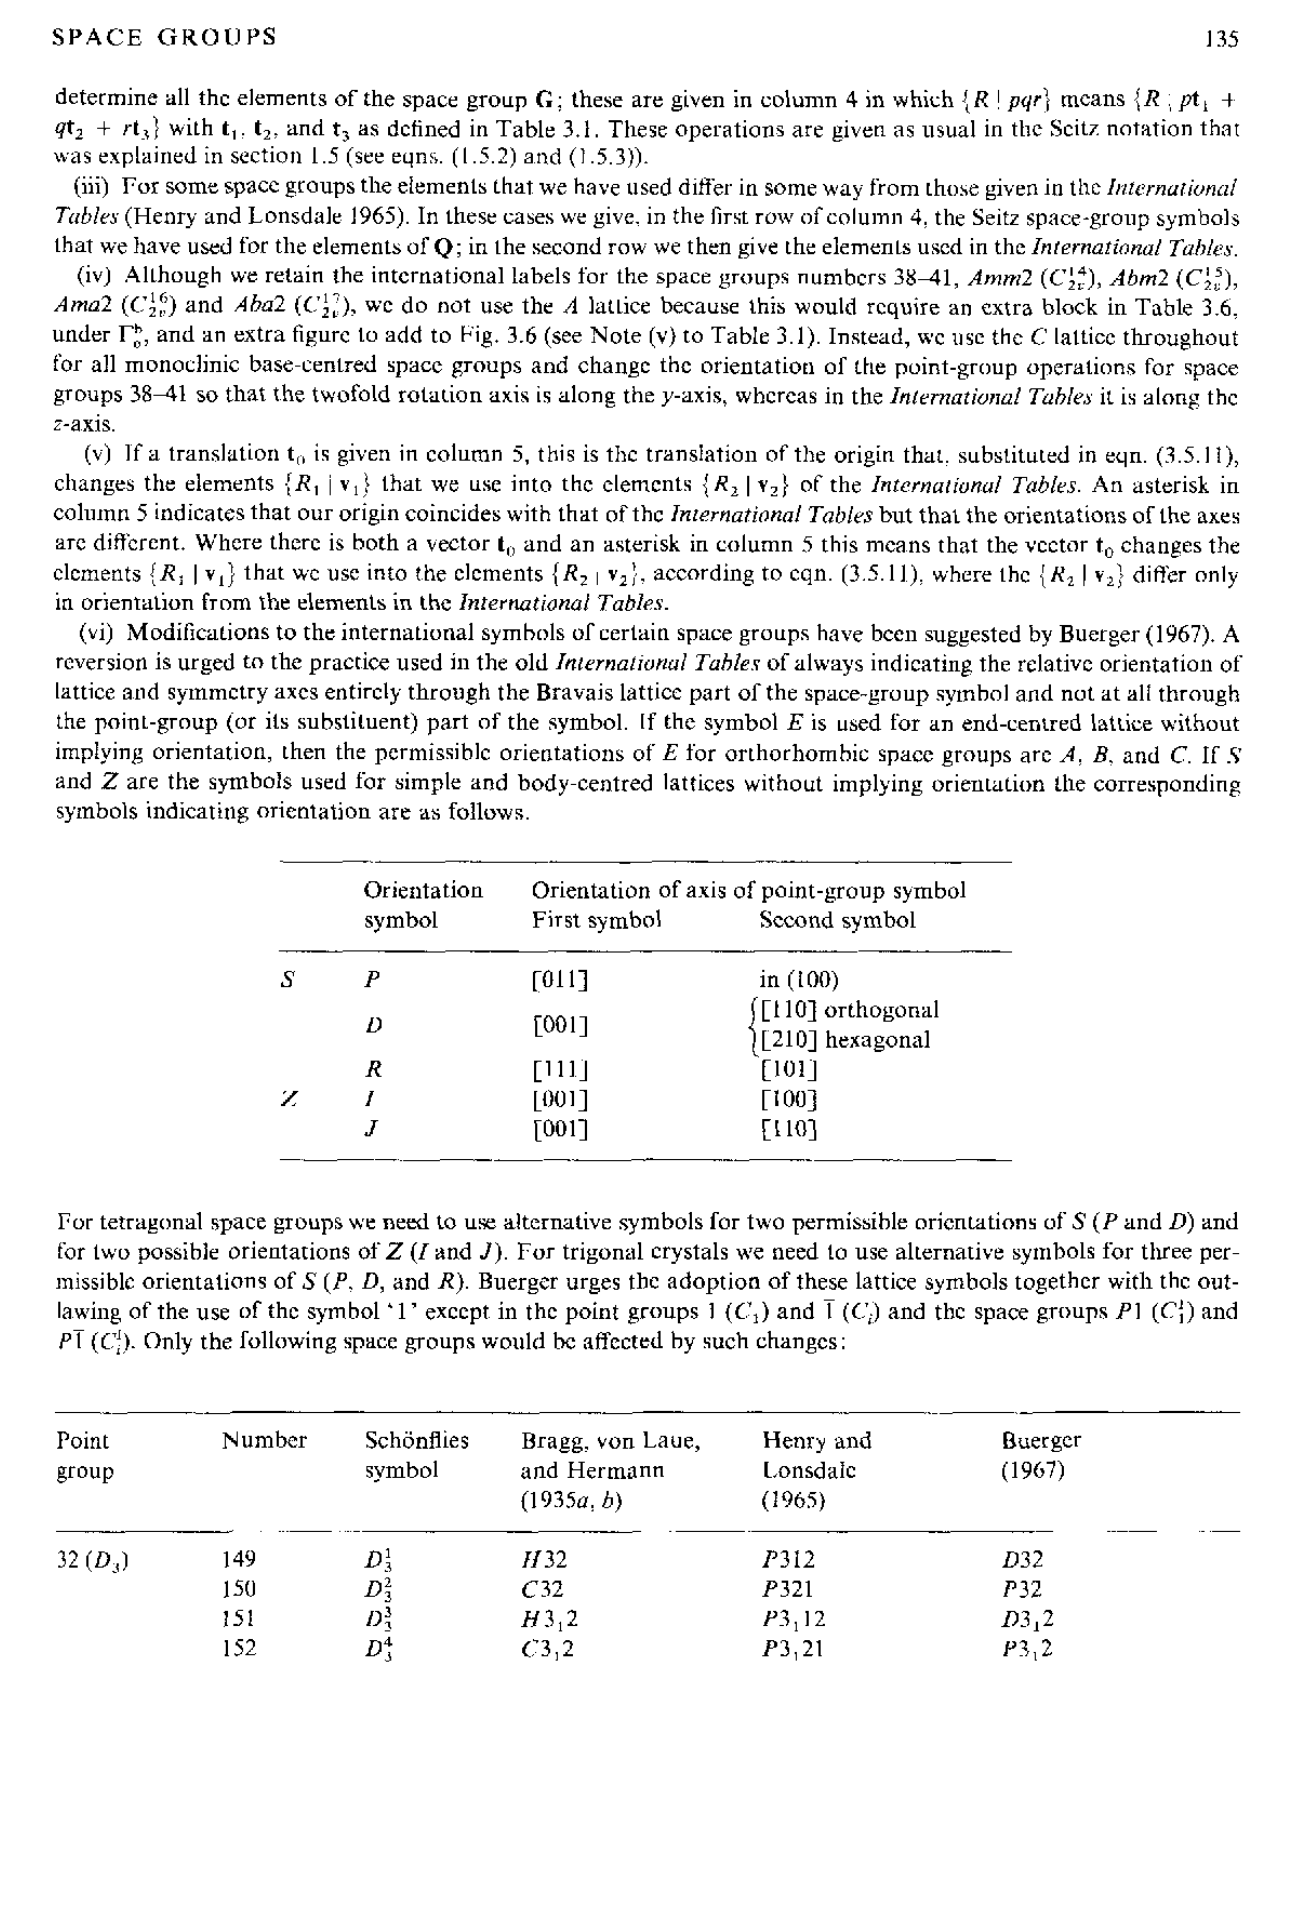
\includegraphics[width=0.92\textwidth]{c3_t37_p9.png}
\caption*{\textbf{表 3.7}（注 (ii) 续--(vi) 及取向符号表，原书扫描）。}
\end{figure}
\begin{figure}[H]
\centering
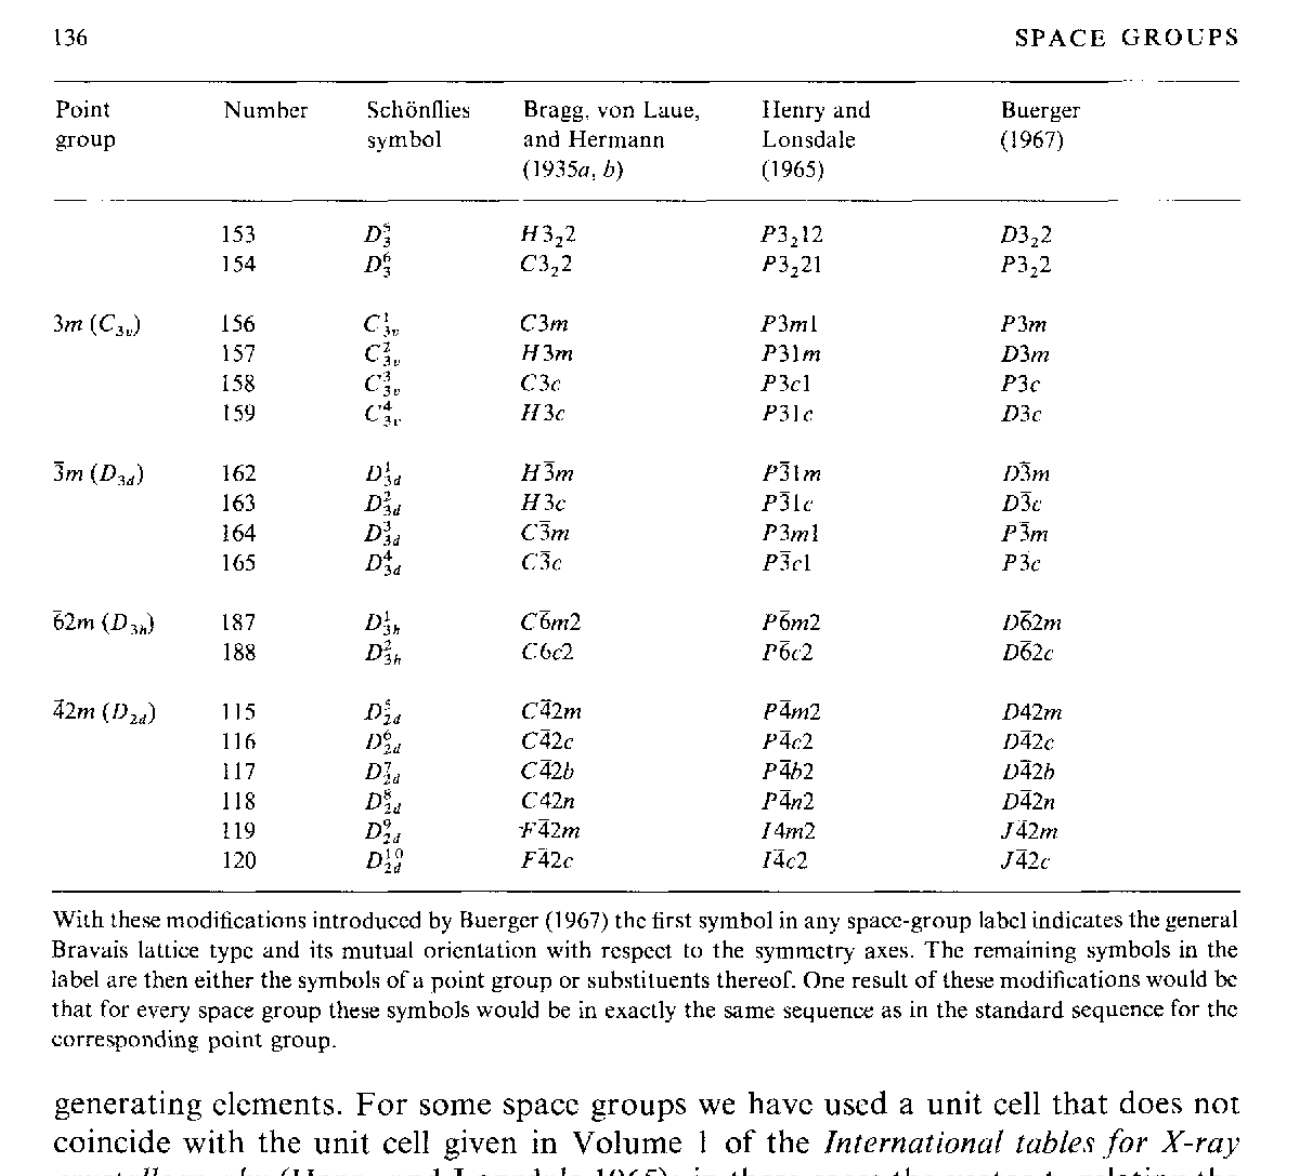
\includegraphics[width=0.80\textwidth]{c3_t37_p10.png}
\caption*{\textbf{表 3.7}（注 (vi) 附表：受 Buerger (1967) 建议影响的空间群，原书扫描）。}
\end{figure}

表 3.7 的注（译文）：

\noindent（i）我们在第 1、2、3 列中分别给出每个空间群的国际编号、国际符号和 Schönflies 符号。第 3 列的 Schönflies 符号前冠以相应布拉维格子的符号（见表 3.1）。

\noindent（ii）第 1、2、3 列给出的空间群名称蕴含（a）它所依托的布拉维格子，以及（b）同形点群。因此无需单独列出平移群 $\mathbf{T}$ 的元素（见表 3.1）或同形点群 $\mathbf{F}$ 的元素（见表 2.2）。尚需给出的是若干陪集代表（即 3.5 节所述 $\mathbf{Q}$ 的元素）。我们给出的数目足以确定空间群 $\mathbf{G}$ 的全部元素；这些元素列于第 4 列，其中 $\{R \mid pqr\}$ 表示 $\{R \mid p\mathbf{t}_{1} + q\mathbf{t}_{2} + r\mathbf{t}_{3}\}$，$\mathbf{t}_{1}$、$\mathbf{t}_{2}$、$\mathbf{t}_{3}$ 按表 3.1 的定义。这些操作一如既往地用 1.5 节解释的 Seitz 记号表示（见式 (1.5.2) 与 (1.5.3)）。

\noindent（iii）对某些空间群，我们所用的元素与《国际表》（Henry and Lonsdale 1965）所给的略有不同。对这些情形，我们在第 4 列的第一行给出我们用于 $\mathbf{Q}$ 的元素的 Seitz 空间群符号，第二行给出《国际表》所用的元素。

\noindent（iv）尽管我们保留编号 38--41（$Amm2\ (C_{2v}^{14})$、$Abm2\ (C_{2v}^{15})$、$Ama2\ (C_{2v}^{16})$、$Aba2\ (C_{2v}^{17})$）的国际记号，但不使用 A 格子，因为那将需要在表 3.6 的 $\Gamma_{o}^{b}$ 之下增加一个条目，并在图 3.6 中增加一幅图（见表 3.1 的注 (v)）。取而代之，我们对所有单斜底心空间群一律使用 C 格子，并把编号 38--41 的点群操作的取向改为使二次转动轴沿 $y$ 轴，而在《国际表》中它沿 $z$ 轴。

\noindent（v）若第 5 列给出一个平移 $\mathbf{t}_{0}$，则把它代入式 (3.5.11) 就能把我们所用的元素 $\{R_{1} \mid \mathbf{v}_{1}\}$ 变换为《国际表》的元素 $\{R_{2} \mid \mathbf{v}_{2}\}$。第 5 列中的星号表示我们的原点与《国际表》的原点重合，但轴的取向不同。若第 5 列既有矢量 $\mathbf{t}_{0}$ 又有星号，则表示矢量 $\mathbf{t}_{0}$ 按式 (3.5.11) 把我们所用的 $\{R_{1} \mid \mathbf{v}_{1}\}$ 变换为 $\{R_{2} \mid \mathbf{v}_{2}\}$，后者与《国际表》的元素只在取向上不同。

\noindent（vi）Buerger（1967）对某些空间群的国际符号提出了修改。他呼吁回到旧版《国际表》的做法：晶格与对称轴的相对取向完全由空间群符号中的布拉维格子部分表明，而完全不通过符号中的点群（或其替代）部分体现。若用符号 E 表示端心格子而不蕴含取向，则正交空间群中 E 的可取取向为 $A$、$B$ 和 $C$。若用 S 和 Z 表示简单和体心格子而不蕴含取向，则表明取向的相应符号如第 9 页扫描图中的表所示。对四方空间群，需要对 $S$ 的两种可取取向（P 和 D）以及 $Z$ 的两种可能取向（I 和 J）使用替代符号；对三方晶体，需要对 $S$ 的三种可取取向（P、D 和 R）使用替代符号。Buerger 敦促采用这些格子符号，并取缔符号“1”的使用——点群 $1\ (C_{1})$ 和 $\bar{1}\ (C_{i})$ 以及空间群 $P1\ (C_{1}^{1})$ 和 $P\bar{1}\ (C_{i}^{1})$ 除外。只有注 (vi) 附表中列出的空间群会受到这些改动的影响。经 Buerger（1967）引入这些修改后，任何空间群标签的第一个符号都表明布拉维格子的一般类型及其相对对称轴的取向，标签中其余的符号则要么是点群符号，要么是其替代符号。这些修改的一个结果是：对每个空间群，这些符号的顺序都将与相应点群的标准顺序完全一致。

空间群本身虽由《国际表》正式定义，但原点的选取和坐标轴取向的选择仍留有若干自由；《国际表》本身对许多空间群就给出了两种可替换的定向，正如 $Pmmn$（$D_{2h}^{13}$）的例子所示。援引《国际表》第 52 页的话：“所采用的空间群标准定向并不具有官方的重要性。”对某些空间群，《新国际表》（Henry and Lonsdale 1965）所用的空间群符号曾受到 Buerger（1967）的批评。Buerger 建议的修改已列于表 3.7 的注 (vi)；若被采纳，将只影响少数空间群。

国际空间群符号的逻辑在 1.5 节已有简要叙述。这些符号用于《国际表》第一版（Bragg, von Laue, and Hermann 1935\textit{a}, \textit{b}）并逐渐通用。当时符号的布拉维格子部分并不完全令人满意，因此在编纂新《国际表》时作了一些修改（Henry and Lonsdale 1965）；表 3.7 采用的就是新版符号。例如，四方点群 $\bar{4}2m$ 放进初基四方布拉维格子的晶胞时，纯转动轴既可以平行于 $x$ 轴，也可以平行于直线 $x = y$。旧《国际表》用两种不同的布拉维格子符号 P 和 C 区分这两种取向；对体心四方格子上的两种取向则用 I 和 F 两种符号。新《国际表》中，同一个布拉维格子在其一切空间群中都用同一符号表示（编号 38--41 的空间群 $Amm2\ (C_{2v}^{14})$、$Abm2\ (C_{2v}^{15})$、$Ama2\ (C_{2v}^{16})$、$Aba2\ (C_{2v}^{17})$ 除外）。点群在布拉维格子上不同取向的区分问题，于是或者通过调换点群符号 $\bar{4}2m$ 和 $\bar{6}2m$ 中最后两个符号的次序（得到 $\bar{4}m2$ 和 $\bar{6}m2$）来解决，或者对三方空间群通过把符号“1”加在空间群符号的不同位置来解决。其结果是，对称性符号如今常常被部分地理解为不仅表明有哪些对称元素，还表明其取向，见 Henry and Lonsdale（1965）的表 3.3.2。国际点群标记各部分的身份问题在第七章还会涉及。

为了说明如何用《国际表》给出的等价位置确定对称元素的几何描述，我们遵循 Wondratschek and Neubüser（1967）的方法。应当从 1.4 与 1.5 节清楚地区分\textit{对称元素}（如转动轴或对称面，粗略地说这是晶体的一种物理属性）与\textit{对称操作}（它是晶体的覆盖操作，是点群或空间群这一抽象数学群的元素）。空间群对称操作 $\{R_{i} \mid \mathbf{r}_{i}\}$ 作用在点 $x, y, z$ 上，产生等价位置中的某一点，后者一般可写为
\begin{equation*}
\begin{aligned}
x', y', z' &= r_{1} + a_{11}x + a_{12}y + a_{13}z,\\
&\quad r_{2} + a_{21}x + a_{22}y + a_{23}z,\ r_{3} + a_{31}x + a_{32}y + a_{33}z,
\end{aligned}
\tag{3.5.14}
\end{equation*}
其中 $r_{i}$ 是有理数，$a_{ij}$ 为 $+1$、$-1$ 或 0。

\noindent\textbf{例 3.5.1}\quad 在 $Pmmn$（$D_{2h}^{13}$）的诸等价位置中有 $\frac{1}{2}+x, \frac{1}{2}-y, \bar{z}$；这意味着 $a_{11} = +1$，$a_{22} = a_{33} = -1$，$r_{1} = r_{2} = \frac{1}{2}$，$r_{3} = 0$，其余 $a_{ij} = 0$。

式 (3.5.14) 可以方便地写成矩阵形式
\begin{equation*}
\mathbf{M}\left(\{R_{i} \mid \mathbf{r}_{i}\}\right) = \begin{pmatrix} a_{11} & a_{12} & a_{13} & r_{1}\\ a_{21} & a_{22} & a_{23} & r_{2}\\ a_{31} & a_{32} & a_{33} & r_{3}\\ 0 & 0 & 0 & 1 \end{pmatrix} = (\mathbf{A}, \mathbf{r}_{i})
\tag{3.5.15}
\end{equation*}
其中 $\mathbf{M}(\{R_{i} \mid \mathbf{r}_{i}\})$ 作用在列矢量 $(x, y, z, 1)^{\mathrm{T}}$ 上。显然矩阵 $a_{ij}$ 已经以缩并的形式出现在表 1.4 的 Jones 符号中。$\{R_{i} \mid \mathbf{r}_{i}\}$ 的 $R_{i}$ 部分的几何意义当然可以直接由表 1.4 辨认；另一种做法是，$\mathbf{A}$ 的特征标 $\chi(\mathbf{A})$ 与行列式 $\det(\mathbf{A})$ 很容易计算，按表 3.8，这两个量完全刻画了 $R_{i}$ 的性质（Bethe 1929），其中 $C_{n}$ 表示转角为 $2\pi/n$ 的转动。

\begin{table}[H]
\centering
\caption*{\textbf{表 3.8}\ 由 $\chi(\mathbf{A})$ 和 $\det(\mathbf{A})$ 确定 $R_{i}$ 的形式}
\begin{tabular}{@{}lcccccccccc@{}}
\toprule
$R_{i}$ & $C_{1}$ & $C_{2}$ & $C_{3}$ & $C_{4}$ & $C_{6}$ & $IC_{1}$ & $IC_{2}$ & $IC_{3}$ & $IC_{4}$ & $IC_{6}$\\
 & & & & & & $\equiv I$ & $\equiv\sigma$ & $\equiv S_{6}$ & $\equiv S_{4}$ & $\equiv S_{3}$\\
\midrule
$\chi(\mathbf{A})$ & $3$ & $-1$ & $0$ & $1$ & $2$ & $-3$ & $1$ & $0$ & $-1$ & $-2$\\
$\det(\mathbf{A})$ & $+1$ & $+1$ & $+1$ & $+1$ & $+1$ & $-1$ & $-1$ & $-1$ & $-1$ & $-1$\\
\bottomrule
\end{tabular}
\end{table}

若 $\det(\mathbf{A}) = +1$，则对称元素或者是纯转动轴，或者是螺旋转动轴。于是我们要确定该轴的方向；对螺旋转动轴，还要确定螺旋矢量 $\mathbf{w}$，即平移 $\mathbf{r}_{i}$ 沿轴方向的分量。若 $\mathbf{q}$ 是过原点且平行于螺旋轴的矢量，则 $\mathbf{A}\mathbf{q} = \mathbf{q}$，因此给出螺旋轴方向的 $\mathbf{q}$ 可由
\begin{equation*}
(\mathbf{A} - \mathbf{E})\mathbf{q} = 0
\tag{3.5.16}
\end{equation*}
求得。对螺旋转动，为确定 $\mathbf{w}$，注意
\begin{equation*}
\{R_{i} \mid \mathbf{r}_{i}\}\mathbf{q} = \mathbf{A}\mathbf{q} + \mathbf{r}_{i} = \mathbf{E}\mathbf{q} + \mathbf{r}_{i} = \mathbf{q} + \mathbf{r}_{i}
\tag{3.5.17}
\end{equation*}
因此
\begin{equation*}
\{R_{i} \mid \mathbf{r}_{i}\}^{2}\mathbf{q} = \mathbf{q} + \mathbf{r}_{i} + \mathbf{A}\mathbf{r}_{i}
\tag{3.5.18}
\end{equation*}
且
\begin{equation*}
\begin{aligned}
\{R_{i} \mid \mathbf{r}_{i}\}^{n}\mathbf{q} &= \mathbf{q} + \mathbf{r}_{i} + \mathbf{A}\mathbf{r}_{i} + \mathbf{A}^{2}\mathbf{r}_{i} + \dots + \mathbf{A}^{n-1}\mathbf{r}_{i}\\
&= \mathbf{q} + n\mathbf{w}
\end{aligned}
\tag{3.5.19}
\end{equation*}
因为 $n$ 次螺旋转动操作等价于纯平移 $n\mathbf{w}$。整理式 (3.5.19) 得螺旋矢量 $\mathbf{w}$ 的显式表达式
\begin{equation*}
\mathbf{w} = (1/n)(\mathbf{E} + \mathbf{A} + \mathbf{A}^{2} + \dots + \mathbf{A}^{n-1})\mathbf{r}_{i}.
\tag{3.5.20}
\end{equation*}
螺旋轴的方向当然由 $\mathbf{w}$ 的方向给出，但由式 (3.5.16) 更容易求得该方向。轴的定位则可由“轴上的点 $\mathbf{x}$ 满足 $\mathbf{A}\mathbf{x} + \mathbf{r}_{i} = \mathbf{x} + \mathbf{w}$”这一事实确定，即
\begin{equation*}
(\mathbf{A} - \mathbf{E})\mathbf{x} = \left(\frac{1}{n}\mathbf{B} - \mathbf{E}\right)\mathbf{r}_{i}
\tag{3.5.21}
\end{equation*}
其中
\begin{equation*}
\mathbf{B} = \mathbf{E} + \mathbf{A} + \mathbf{A}^{2} + \dots + \mathbf{A}^{n-1}.
\tag{3.5.22}
\end{equation*}
若 $n = 2$，式 (3.5.21) 有特别简单的解 $\mathbf{x} = \frac{1}{2}\mathbf{r}_{i}$。若 $\det(\mathbf{A}) = -1$，则要考虑三种可能的情形：(a) $I\ ( = IC_{1})$；(b) $\sigma\ ( = IC_{2})$；(c) $S_{6}\ ( = IC_{3})$；$S_{4}\ ( = IC_{4})$；以及 $S_{3}\ ( = IC_{6})$。

\noindent(a) $I\ ( = IC_{1})$。反演中心 $\mathbf{x}$ 可由 $\mathbf{x} = \{I \mid \mathbf{r}_{i}\}\mathbf{x} = -\mathbf{x} + \mathbf{r}_{i}$ 求得，故 $\mathbf{x} = \frac{1}{2}\mathbf{r}_{i}$。

\noindent(b) $\sigma\ ( = IC_{2})$。平面的取向可以用一个过原点且垂直于该平面的矢量 $\mathbf{q}$ 描述；$\mathbf{q}$ 满足 $\mathbf{A}\mathbf{q} = -\mathbf{q}$，即
\begin{equation*}
(\mathbf{A} + \mathbf{E})\mathbf{q} = 0.
\tag{3.5.23}
\end{equation*}
对滑移面，滑移矢量 $\mathbf{w}$ 可由下述事实求得：把 $\{R_{i} \mid \mathbf{r}_{i}\}$ 相继作用两次于平面内的点 $\mathbf{x}$，把它移到 $\mathbf{x} + 2\mathbf{w}$，于是由式 (3.5.18)，
\begin{equation*}
\{R_{i} \mid \mathbf{r}_{i}\}^{2}\mathbf{x} = \mathbf{x} + \mathbf{r}_{i} + \mathbf{A}\mathbf{r}_{i} = \mathbf{x} + 2\mathbf{w}.
\tag{3.5.24}
\end{equation*}
因此
\begin{equation*}
\mathbf{w} = \frac{1}{2}(\mathbf{A} + \mathbf{E})\mathbf{r}_{i}.
\tag{3.5.25}
\end{equation*}
平面内任一点 $\mathbf{x}$ 满足 $\{R_{i} \mid \mathbf{r}_{i}\}\mathbf{x} = \mathbf{A}\mathbf{x} + \mathbf{r}_{i} = \mathbf{x} + \mathbf{w}$，故 $\mathbf{x}$ 满足
\begin{equation*}
(\mathbf{A} - \mathbf{E})\mathbf{x} = \frac{1}{2}(\mathbf{A} - \mathbf{E})\mathbf{r}_{i},
\tag{3.5.26}
\end{equation*}
它显然有特解 $\mathbf{x} = \frac{1}{2}\mathbf{r}_{i}$。

\noindent(c) $S_{6}\ ( = IC_{3})$；$S_{4}\ ( = IC_{4})$；$S_{3}\ ( = IC_{6})$。若 $\mathbf{q}$ 是过原点且平行于其中某根轴的矢量，则 $\mathbf{A}\mathbf{q} = -\mathbf{q}$，$\mathbf{q}$ 同样由求解
\begin{equation*}
(\mathbf{A} + \mathbf{E})\mathbf{q} = 0.
\tag{3.5.23}
\end{equation*}
得到。\footnote{中译者注：原书对情形 (b) 与 (c) 重复使用了编号 (3.5.23)，照录。}不存在螺旋矢量 $\mathbf{w}$。反演中心可由 $\{R_{i} \mid \mathbf{r}_{i}\}\mathbf{x} = \mathbf{A}\mathbf{x} + \mathbf{r}_{i} = \mathbf{x}$ 求得，即
\begin{equation*}
(\mathbf{E} - \mathbf{A})\mathbf{x} = \mathbf{r}_{i}.
\tag{3.5.27}
\end{equation*}

在《国际表》中每个矩阵 $\mathbf{A}$ 都属于表 3.9 所示的四种不同类型之一。确定了 $R_{i}$ 的形式和 $\mathbf{A}$ 的类型之后，就可以利用表 3.10（它用到式 (3.5.16)--(3.5.27)）来确定与《国际表》中该空间群每个等价位置相对应的对称元素的取向和位置。

\begin{table}[H]
\centering
\caption*{\textbf{表 3.9}\ 由《X 射线晶体学国际表》产生的矩阵 $\mathbf{A}$ 的类型}
\begin{tabular}{@{}ll@{}}
\toprule
(i) & $\mathbf{A} = \begin{pmatrix} +1 & 0 & 0\\ 0 & \pm 1 & 0\\ 0 & 0 & \pm 1 \end{pmatrix}$；\qquad
(iii) (a) $\mathbf{A} = \begin{pmatrix} 0 & 0 & \pm 1\\ +1 & 0 & 0\\ 0 & \pm 1 & 0 \end{pmatrix}$，\\[3ex]
(ii) (a) & $\mathbf{A} = \begin{pmatrix} \pm 1 & 0 & 0\\ 0 & 0 & \pm 1\\ 0 & -1 & 0 \end{pmatrix}$，\qquad\quad
(b) $\mathbf{A} = \begin{pmatrix} 0 & \pm 1 & 0\\ 0 & 0 & \pm 1\\ +1 & 0 & 0 \end{pmatrix}$；\\[3ex]
(b) & $\mathbf{A} = \begin{pmatrix} 0 & 0 & \pm 1\\ 0 & \pm 1 & 0\\ \pm 1 & 0 & 0 \end{pmatrix}$，\qquad\quad
(iv) $\mathbf{A} = \begin{pmatrix} a_{11} & a_{12} & 0\\ a_{21} & a_{22} & 0\\ 0 & 0 & \pm 1 \end{pmatrix}$\quad
其中有一个 $a_{ik} = 0$，\\
\multicolumn{2}{l}{其余三个 $a_{ik} = \pm 1$；$i, k = 1, 2$。}\\
\bottomrule
\end{tabular}
\end{table}

\noindent\textbf{表 3.9 的注}\quad（i）假定采用的是 Henry and Lonsdale（1965）给出的定向；对其他定向，将不得不求解式 (3.5.16)--(3.5.27) 中的相应方程。

\begin{figure}[H]
\centering
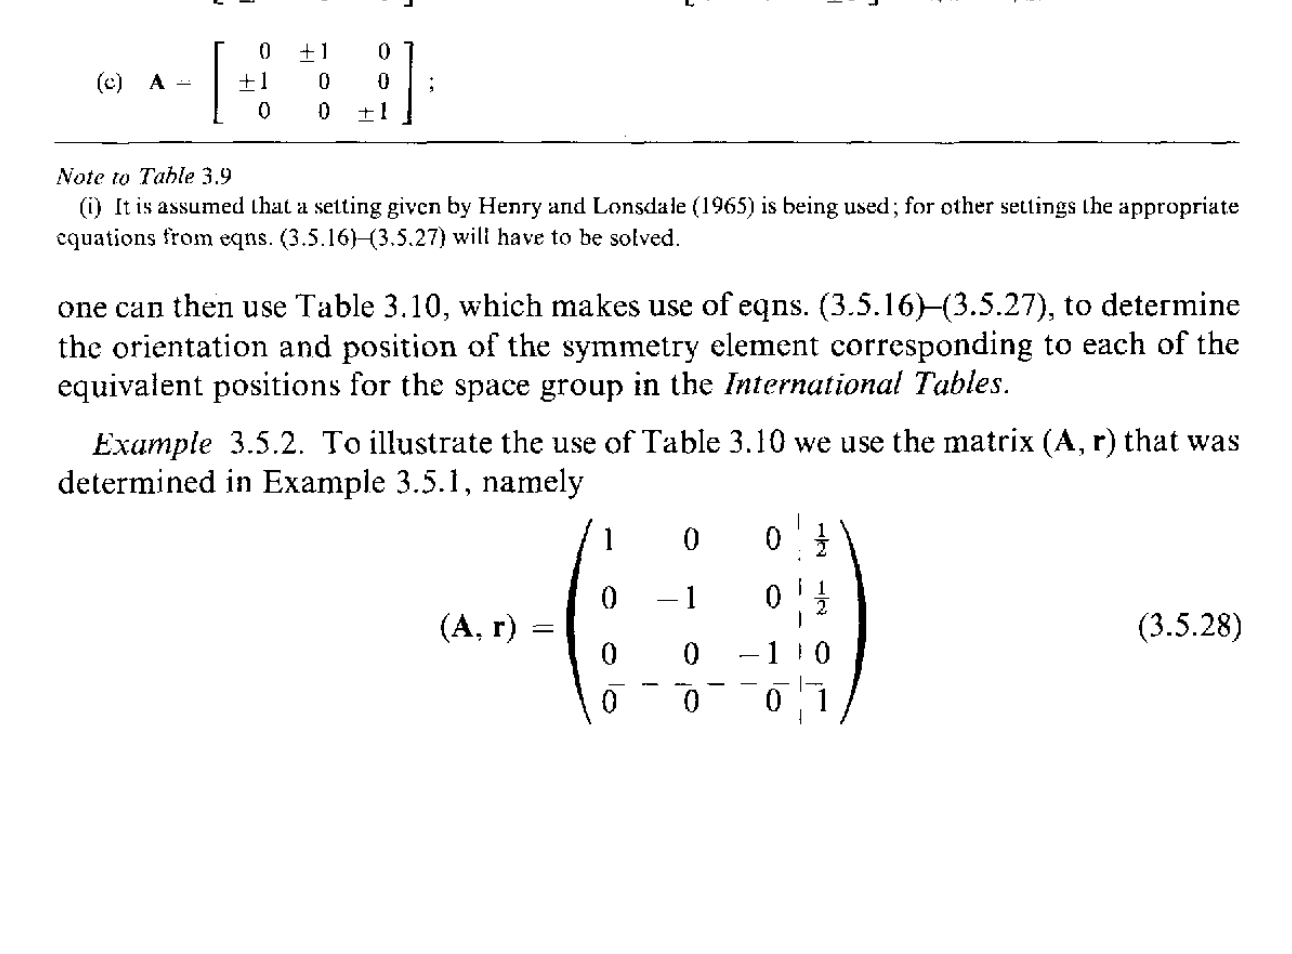
\includegraphics[width=0.92\textwidth]{c3_t310_p1.png}
\caption*{\textbf{表 3.10}\ 对称元素的测定（据 Wondratschek and Neubüser (1967)，原书第 140 页起扫描；第 1 页）。}
\end{figure}
\begin{figure}[H]
\centering
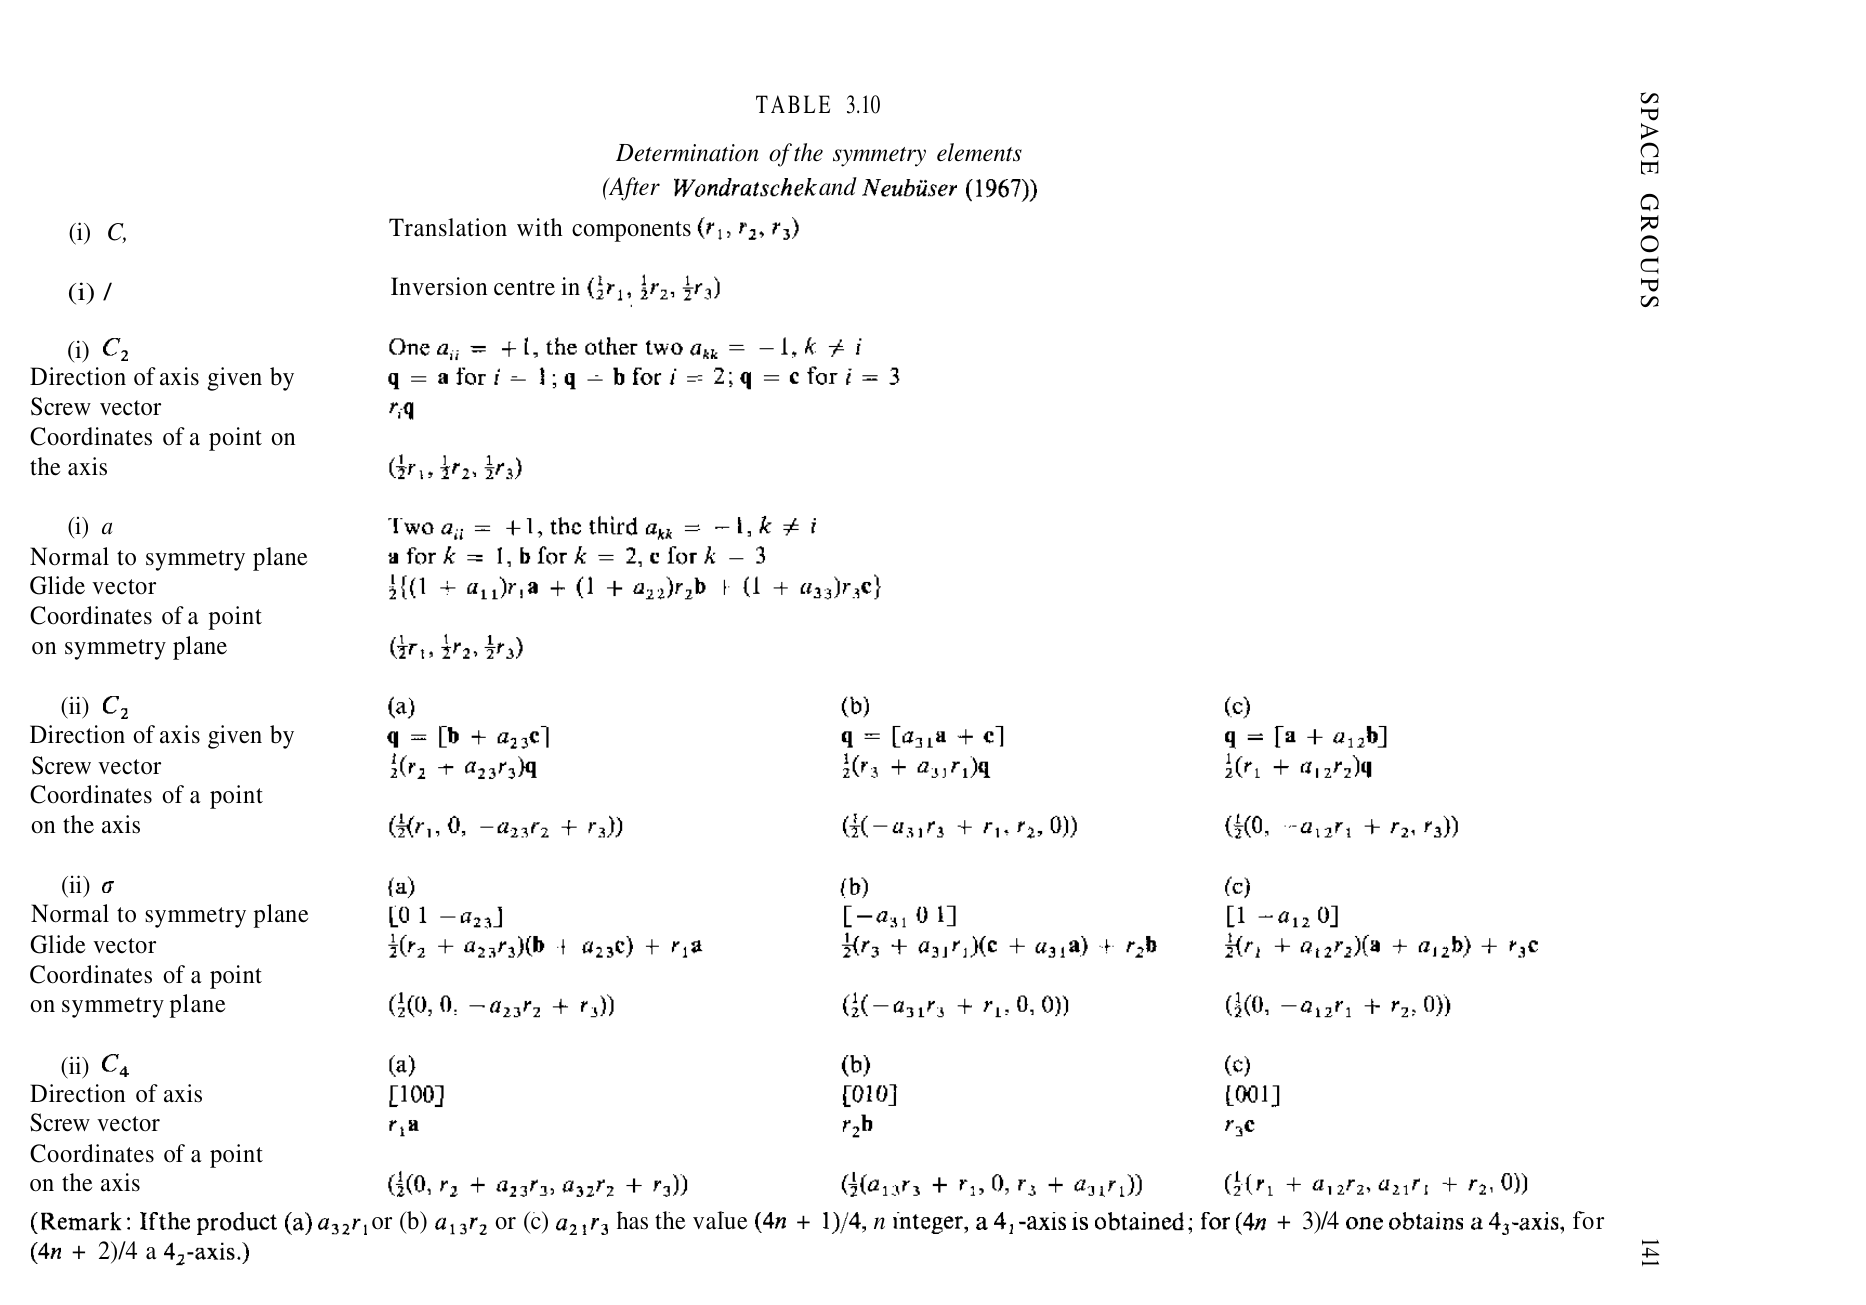
\includegraphics[width=0.92\textwidth]{c3_t310_p2.png}
\caption*{\textbf{表 3.10}（第 2 页）。}
\end{figure}
\begin{figure}[H]
\centering
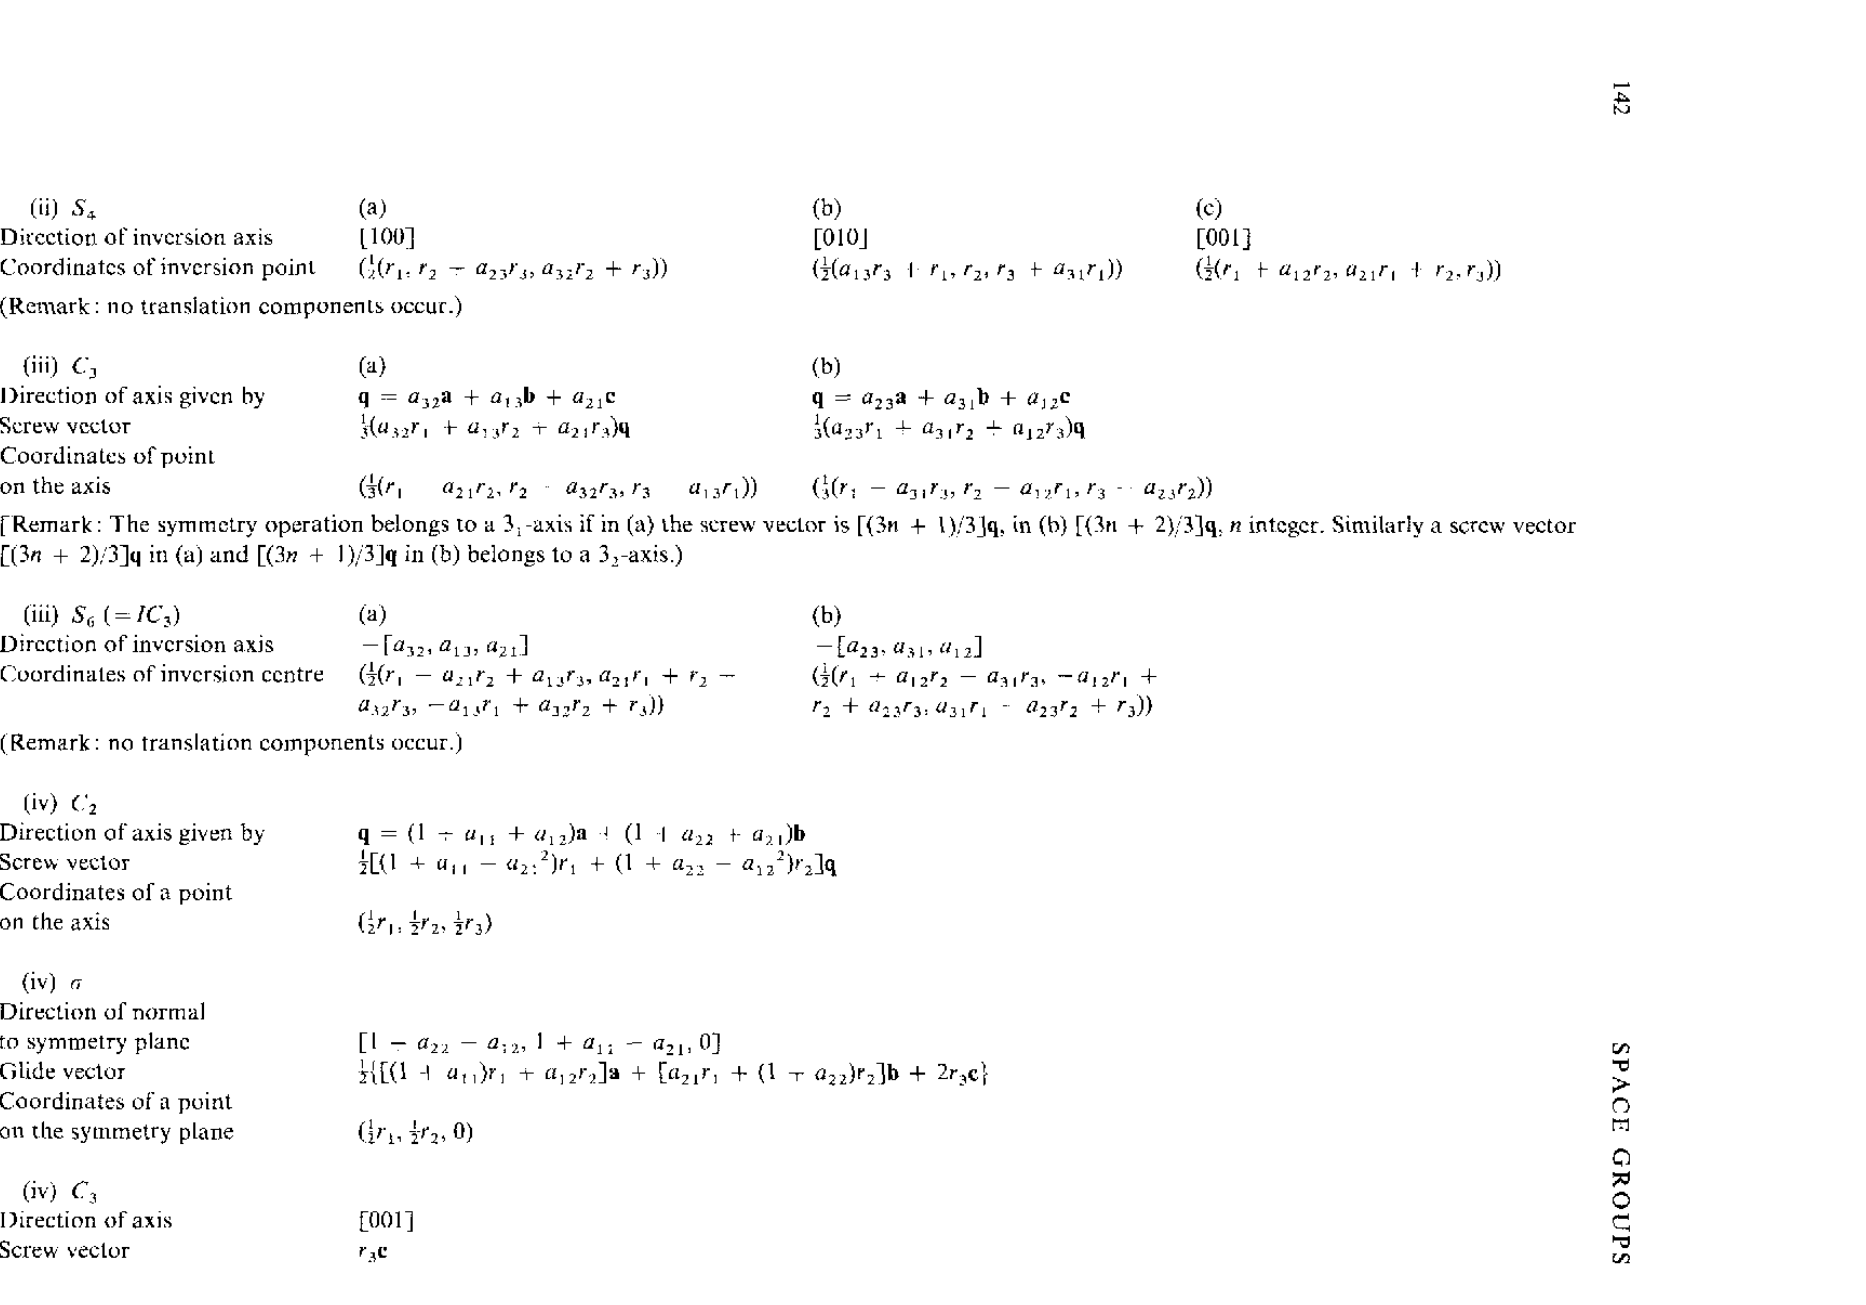
\includegraphics[width=0.92\textwidth]{c3_t310_p3.png}
\caption*{\textbf{表 3.10}（第 3 页，页末为表的注）。}
\end{figure}

表 3.10 的注（译文）：

\noindent（i）与《国际表》一致，$a$、$b$、$c$ 是惯用晶胞交于一个顶点的三条棱的长度；$\mathbf{a}$、$\mathbf{b}$、$\mathbf{c}$ 是沿这些棱的矢量。

\noindent（ii）矩阵 $\mathbf{A}(a_{ij})$ 与矢量 $\mathbf{r}_{i}$ 在正文中定义，见式 (3.5.14) 与 (3.5.15)。

\noindent（iii）$\mathbf{A}$ 的类型（i）、（ii）、（iii）或（iv）要用表 3.9 确定。

\noindent（iv）$C_{n}$ 是转角为 $2\pi/n$ 的纯转动。

\noindent（v）本表适用于 Henry and Lonsdale（1965）给出的晶胞定向；对其他定向，将不得不求解式 (3.5.16)--(3.5.27) 中的相应方程。

\noindent\textbf{例 3.5.2}\quad 为了说明表 3.10 的用法，我们用在例 3.5.1 中确定的矩阵 $(\mathbf{A}, \mathbf{r})$：
\begin{equation*}
(\mathbf{A}, \mathbf{r}) = \begin{pmatrix} 1 & 0 & 0 & \frac{1}{2}\\ 0 & -1 & 0 & \frac{1}{2}\\ 0 & 0 & -1 & 0\\ 0 & 0 & 0 & 1 \end{pmatrix}
\tag{3.5.28}
\end{equation*}
于是
\begin{equation*}
\mathbf{A} = \begin{pmatrix} 1 & 0 & 0\\ 0 & -1 & 0\\ 0 & 0 & -1 \end{pmatrix}
\tag{3.5.29}
\end{equation*}
从而
\begin{equation*}
\chi(\mathbf{A}) = -1
\tag{3.5.30}
\end{equation*}
且
\begin{equation*}
\det(\mathbf{A}) = +1.
\tag{3.5.31}
\end{equation*}
由表 3.8，$\{R_{i} \mid \mathbf{r}_{i}\}$ 是一个 $C_{2}$ 型转动；再由表 3.10，由于 $i = 1$，它沿 $x$ 方向，即 $C_{2x}$。螺旋矢量的方向为 $\mathbf{r}_{1}\mathbf{q} = \frac{1}{2}\mathbf{a}$，轴的位置由其通过点 $\left(\frac{1}{2}r_{1}, \frac{1}{2}r_{2}, \frac{1}{2}r_{3}\right)$，即通过 $(\frac{1}{4}a, \frac{1}{4}b, 0)$ 这一事实确定。

% 3.6 空间群操作对 Bloch 函数的作用
\section{空间群操作对 Bloch 函数的作用}

现在我们讨论把空间群算符作用于 Bloch 函数所产生的效果。由于本书采用主动操作，1.5 节关于函数空间算符的讨论给出
\begin{equation*}
\{S \mid \mathbf{w}\}\psi(\mathbf{r}) = \psi(S^{-1}(\mathbf{r} - \mathbf{w}))
\tag{3.6.1}
\end{equation*}
其中我们省去了函数空间算符的下标 \textit{a} 和上横线。

首先证明
\begin{equation*}
\exp(\mathrm{i}\mathbf{k} \cdot S\mathbf{r}) = \exp(\mathrm{i}S^{-1}\mathbf{k} \cdot \mathbf{r}).
\tag{3.6.2}
\end{equation*}
这是因为
\begin{equation*}
\mathbf{k} \cdot S\mathbf{r} = \sum_{i}\sum_{j}k_{i}S_{ij}r_{j} = \sum_{i}\sum_{j}S^{\mathrm{T}}_{ji}k_{i}r_{j} = \sum_{i}\sum_{j}S^{-1}_{ji}k_{i}r_{j},
\tag{3.6.3}
\end{equation*}
因为 $S_{ij}$ 是正交矩阵。这意味着由式 (3.6.1) 与 (3.6.2)，
\begin{equation*}
\begin{aligned}
\{S \mid \mathbf{w}\}\exp(\mathrm{i}\mathbf{k} \cdot \mathbf{r}) &= \exp\left\{\mathrm{i}\mathbf{k} \cdot S^{-1}(\mathbf{r} - \mathbf{w})\right\}\\
&= \exp\left\{\mathrm{i}S\mathbf{k} \cdot (\mathbf{r} - \mathbf{w})\right\},
\end{aligned}
\tag{3.6.4}
\end{equation*}
它几乎就是同一个函数，只是以倒格矢 $S\mathbf{k}$ 标记，且中心位于 $\mathbf{r} = \mathbf{w}$。

类似地可以定义
\begin{equation*}
u_{S\mathbf{k}}(\mathbf{r} - \mathbf{w}) = u_{\mathbf{k}}\left\{S^{-1}(\mathbf{r} - \mathbf{w})\right\} = \{S \mid \mathbf{w}\}u_{\mathbf{k}}(\mathbf{r}),
\tag{3.6.5}
\end{equation*}
其中 $u_{\mathbf{k}}(\mathbf{r})$ 满足式 (3.4.8)，即它具有格子的周期性。联立式 (3.6.4) 与 (3.6.5) 并利用 Bloch 函数的定义
\begin{equation*}
\Psi_{\mathbf{k}}(\mathbf{r}) = \exp(\mathrm{i}\mathbf{k} \cdot \mathbf{r})\,u_{\mathbf{k}}(\mathbf{r}),
\tag{3.4.7}
\end{equation*}
得到
\begin{equation*}
\begin{aligned}
\{S \mid \mathbf{w}\}\psi_{\mathbf{k}}(\mathbf{r}) &= \exp\left\{\mathrm{i}S\mathbf{k} \cdot (\mathbf{r} - \mathbf{w})\right\}u_{S\mathbf{k}}(\mathbf{r} - \mathbf{w})\\
&= \psi_{S\mathbf{k}}(\mathbf{r} - \mathbf{w}),
\end{aligned}
\tag{3.6.6}
\end{equation*}
姑且如此记。又由式 (1.5.24) 可得
\begin{equation*}
\{S \mid \mathbf{w}\}\{R \mid \mathbf{v}\}\psi_{\mathbf{k}}(\mathbf{r}) = \psi_{SR\mathbf{k}}(\mathbf{r} - \mathbf{w} - S\mathbf{v}).
\tag{3.6.7}
\end{equation*}
应当注意 $u_{S\mathbf{k}}$ 也满足式 (3.4.8)，因为若 $\mathbf{t}$ 是一个平移，则 $\mathbf{t}' = S^{-1}\mathbf{t}$ 也是，于是
\begin{equation*}
\begin{aligned}
u_{S\mathbf{k}}(\mathbf{r} - \mathbf{w} + \mathbf{t}) &= u_{\mathbf{k}}\left\{S^{-1}(\mathbf{r} - \mathbf{w} + \mathbf{t})\right\}\\
&= u_{\mathbf{k}}\left\{S^{-1}(\mathbf{r} - \mathbf{w}) + \mathbf{t}'\right\}\\
&= u_{\mathbf{k}}\left\{S^{-1}(\mathbf{r} - \mathbf{w})\right\}\quad\text{（由式 (3.4.8)）}\\
&= u_{S\mathbf{k}}(\mathbf{r} - \mathbf{w}).
\end{aligned}
\tag{3.6.8}
\end{equation*}
这意味着式 (3.6.6) 的右端是一个 Bloch 函数。于是，$\{S \mid \mathbf{w}\}$ 作用在以波矢 $\mathbf{k}$ 标记、中心位于 $\mathbf{r} = 0$ 的 Bloch 函数上，把它变换为以波矢 $S\mathbf{k}$ 标记、中心位于 $\mathbf{r} = \mathbf{w}$ 的 Bloch 函数。尽管式 (3.6.4) 与 (3.6.6) 十分相似，二者之间有一个重要差别。若 $S\mathbf{k} = \mathbf{k}$，则 $\{S \mid \mathbf{w}\}\exp(\mathrm{i}\mathbf{k} \cdot \mathbf{r}) = \exp\left\{\mathrm{i}\mathbf{k} \cdot (\mathbf{r} - \mathbf{w})\right\}$，它是完全相同的函数，只是中心位于 $\mathbf{r} = \mathbf{w}$。然而若 $S\mathbf{k} \equiv \mathbf{k}$（等价），则不一定有 $\{S \mid \mathbf{w}\}\psi_{\mathbf{k}}(\mathbf{r}) = \psi_{\mathbf{k}}(\mathbf{r} - \mathbf{w})$；这是因为 $\psi_{\mathbf{k}}(\mathbf{r})$ 上的标记 $\mathbf{k}$ 只是在等价意义下确定的。一个例子有助于说明这一点。设 $\mathbf{k} = \mathbf{0}$，则 $S\mathbf{k} = \mathbf{k}$ 平凡地成立；再取 $\psi_{0}(\mathbf{r}) = 1 + \exp(\mathrm{i}\mathbf{g} \cdot \mathbf{r})$，于是由式 (3.6.5)，
\begin{equation*}
\begin{aligned}
\{S \mid \mathbf{w}\}\psi_{0}(\mathbf{r}) &= \psi_{0}(S^{-1}\mathbf{r} - S^{-1}\mathbf{w})\\
&= 1 + \exp\left\{\mathrm{i}\mathbf{g} \cdot S^{-1}(\mathbf{r} - \mathbf{w})\right\}\\
&= 1 + \exp\left\{\mathrm{i}S\mathbf{g} \cdot (\mathbf{r} - \mathbf{w})\right\}.
\end{aligned}
\tag{3.6.9}
\end{equation*}
但式 (3.6.9) 的右端等于 $\psi_{0}(\mathbf{r} - \mathbf{w})$ 仅当 $S\mathbf{g} = \mathbf{g}$ 时成立。然而，由于 $S\mathbf{g}$ 与 $\mathbf{g}$ 等价，而后者又与零等价，所以与式 (3.6.9) 右端相联系的波矢仍然是零矢量。

\noindent\textbf{定理 3.6.1}\quad 若 $\psi_{\mathbf{k}}(\mathbf{r})$ 是波矢为 $\mathbf{k}$ 的 Bloch 函数，即 $\{E \mid \mathbf{t}\}\psi_{\mathbf{k}}(\mathbf{r}) = \exp(-\mathrm{i}\mathbf{k} \cdot \mathbf{t})\psi_{\mathbf{k}}(\mathbf{r})$，则 $\{S \mid \mathbf{w}\}\psi_{\mathbf{k}}(\mathbf{r})$ 是波矢为 $S\mathbf{k}$ 的 Bloch 函数。

读者应当明白，这并不是通过把 $\{E \mid \mathbf{t}\}$ 作用于式 (3.6.6) 两端并利用已知事实“$\psi_{S\mathbf{k}}(\mathbf{r} - \mathbf{w})$ 是波矢为 $S\mathbf{k}$ 的 Bloch 函数”就能得到的，因为式 (3.6.6) 是数值关系而非函数关系。要在解析上证明该定理，需要经过下面一系列等式：
\begin{equation*}
\begin{aligned}
\{E \mid \mathbf{t}\}\{S \mid \mathbf{w}\}\psi_{\mathbf{k}}(\mathbf{r}) &= \{S \mid \mathbf{w}\}\psi_{\mathbf{k}}(\mathbf{r} - \mathbf{t})\\
&= \psi_{\mathbf{k}}\left\{S^{-1}(\mathbf{r} - \mathbf{t} - \mathbf{w})\right\} = \psi_{S\mathbf{k}}(\mathbf{r} - \mathbf{t} - \mathbf{w})\\
&= \{E \mid \mathbf{t}\}\psi_{S\mathbf{k}}(\mathbf{r} - \mathbf{w}) = \exp(-\mathrm{i}S\mathbf{k} \cdot \mathbf{t})\psi_{S\mathbf{k}}(\mathbf{r} - \mathbf{w})\\
&= \exp(-\mathrm{i}S\mathbf{k} \cdot \mathbf{t})\{S \mid \mathbf{w}\}\psi_{\mathbf{k}}(\mathbf{r}).
\end{aligned}
\tag{3.6.10}
\end{equation*}
当然，也可以从式 (3.6.6) 出发、借助对 Bloch 周期性的几何直观来论证这个定理。作为定理的推论：若 $S\mathbf{k} = \mathbf{k}$，则 $\{S \mid \mathbf{w}\}\psi_{\mathbf{k}}(\mathbf{r})$ 是波矢为 $\mathbf{k}$ 的 Bloch 函数。我们在下一节将用到这个定理。

% 3.7 空间群表示理论的描述性叙述
\section{空间群表示理论的描述性叙述}

本节描述如何求出给定空间群的所有表示。这里的叙述并不完全严格；论证中的主要缺口在文中均有指出。这些缺口将在第四章补齐，该章对具有真不变 Abel 子群的群的表示理论给出严格而完整的论述，空间群正是这类群的一个特例。

于是我们考虑具有平移子群 $\mathbf{T}$ 的空间群 $\mathbf{G}$。$\mathbf{T}$ 的表示已在 3.4 节给出，它们由 $\mathbf{G}$ 所依托的布拉维格子 $\mathbf{F}$ 的布里渊区中的矢量 $\mathbf{k}$ 刻画。这些表示 $\Delta^{\mathbf{k}}$ 满足（见式 (3.4.3)）
\begin{equation*}
\Delta^{\mathbf{k}}(\{E \mid \mathbf{t}\}) = \exp(-\mathrm{i}\mathbf{k} \cdot \mathbf{t}).
\tag{3.7.1}
\end{equation*}
我们可以用 $\mathbf{T}$ 的左陪集代表写出 $\mathbf{G}$：
\begin{equation*}
\mathbf{G} = \{R_{1} \mid \mathbf{v}_{1}\}\mathbf{T} + \{R_{2} \mid \mathbf{v}_{2}\}\mathbf{T} + \dots + \{R_{h} \mid \mathbf{v}_{h}\}\mathbf{T}
\tag{3.5.2}
\end{equation*}
其中一如既往可取 $R_{1} = E$、$\mathbf{v}_{1} = 0$，而 $\mathbf{v}_{i}$ 是与 $R_{i}$ 相联系的矢量。陪集代表构成集合 $\mathbf{Q}$，它不一定是群。然而商群 $\mathbf{G}/\mathbf{T}$ 是群，且同构于由算符 $R_{1}, R_{2}, \dots, R_{h}$ 构成的点群 $\mathbf{F}$。$\mathbf{F}$ 是 $\mathbf{G}$ 的同形点群，其阶 $h$ 是 $\mathbf{G}$ 的宏观阶。

\noindent\textbf{定义 3.7.1}\quad （表示域）\ 对任何空间群 $\mathbf{G}$，相应布里渊区存在一个\textit{表示域}（representation domain）$\Phi$，使得 $(\sum_{R} R\Phi)$ 等于整个布里渊区，其中对 $R$ 的求和取遍 $\mathbf{G}$ 的同形点群 $\mathbf{F}$ 的元素。

把表示域的这一定义与定义 3.3.3 中基本域的定义加以比较是有益的。若空间群 $\mathbf{G}$ 的同形点群就是相应晶系的全对称点群，即 $\mathbf{F}$ 与 $\mathbf{P}$ 重合，则表示域 $\Phi$ 与基本域 $\Omega$ 体积相同，并且可以取成彼此重合。但一般地 $\mathbf{F}$ 是 $\mathbf{P}$ 的子群；若 $|\mathbf{P}|/|\mathbf{F}| = i$，则表示域 $\Phi$ 的体积将等于基本域 $\Omega$ 体积的 $i$ 倍。还要注意，尽管 $\Omega$ 对每个布里渊区是固定的，$\Phi$ 却依赖于所考虑的空间群。对给定空间群 $\mathbf{G}$ 引入 $\Phi$ 的原因在于，它在推导 $\mathbf{G}$ 的完全表示集合的方案中至关重要。

作为抽象数学问题，确定空间群 $\mathbf{G}$ 的表示是有趣的。然而，研究空间群表示的动机大多与它们在研究规则晶体中量子力学粒子或准粒子的哈密顿量的本征函数和本征值方面的用处有关。众所周知（也许近平凡）的一个说法是：若系统具有某群对称操作 $\mathbf{G}$，则该系统的任何物理可观察量也必具有这些对称操作；这一说法有时称为 Neumann 原理，例如用于简化描述晶体某种物理性质的张量的形式（Birss 1964, Nye 1957）。然而波函数 $\psi$ 不是系统的物理可观察量，因此不能必然地期望它展现 $\mathbf{G}$ 的全部对称性。尽管如此，仍然可以获得关于 $\psi$ 在 $\mathbf{G}$ 元素操作下的变换性质的若干信息。把群论应用于量子力学研究的基本原理在于 1.1 节提到的 Wigner 定理；该定理有若干种表述方式，这里只给出一种。

\noindent\textbf{定理 3.7.1}\quad （Wigner 定理）\ 若 $R$ 是描述某个量子力学系统的哈密顿算符 $H$ 的对称操作，且 $\psi$ 是 $H$ 的本征函数，则 $R\psi$ 也是 $H$ 的本征函数，并与 $\psi$ 具有相同的本征值 $E$。

关于该定理的证明，读者可参考 Wigner 关于群论与量子力学的经典著作（英译本 Wigner (1959)）。这一结果的另一种说法是：粒子或准粒子的波函数 $\psi$ 必定是 $\mathbf{G}$ 的某个不可约表示的基的一个分量。在我们眼下的问题中 $\mathbf{G}$ 是空间群。

现在我们采用的方法是：假设给定 $\mathbf{G}$ 的任意一个表示，讨论它的性质；然后假设我们找到的性质不仅必要而且足以刻画 $\mathbf{G}$ 的表示——这一假设是使本处理不完全严格的原因之一。做完这些之后，我们将说明如何系统地构造出 $\mathbf{G}$ 的所有表示。

设 $\Gamma$ 是作用在维数为 $d$ 的矢量空间 $V$ 上的 $\mathbf{G}$ 的表示。若只考虑 $\Gamma$ 中表示平移的那些元素，则它们构成 $\mathbf{T}$ 的一个表示，它一般是可约的。设它约化成由矢量 $\mathbf{k}_{1}, \mathbf{k}_{2}, \dots, \mathbf{k}_{q}$ 刻画的 $\mathbf{T}$ 的表示。这些 $\mathbf{T}$ 的表示都是一维的，于是由 3.4 节的讨论可知，在 $V$ 中可以找到一组由 Bloch 函数 $\psi_{\mathbf{k}_{1}}(\mathbf{r}), \psi_{\mathbf{k}_{2}}(\mathbf{r}), \dots, \psi_{\mathbf{k}_{d}}(\mathbf{r})$ 构成的基，相对于这组基，$\mathbf{T}$ 的元素由对角矩阵表示；且由式 (3.7.1)，对角元 $\Gamma(\{E \mid \mathbf{t}\})_{pp}$ 为 $\exp(-\mathrm{i}\mathbf{k}_{p} \cdot \mathbf{t})$。矢量 $\mathbf{k}_{1}, \mathbf{k}_{2}, \dots, \mathbf{k}_{d}$ 可能不全不同；此时需要对函数 $\psi_{\mathbf{k}_{p}}(\mathbf{r})$ 引入第二个指标，以区分用同一 $\mathbf{k}$ 矢量标记的两个函数。为了考察这是否可能，让我们仔细考察矢量 $\mathbf{k}_{1}, \mathbf{k}_{2}, \dots, \mathbf{k}_{d}$ 最初是如何产生的。我们利用两个事实：$V$ 在 $\mathbf{G}$ 下不可约；以及定理 3.6.1——若 $\psi_{\mathbf{k}}(\mathbf{r})$ 是波矢为 $\mathbf{k}$ 的 Bloch 函数，则 $\{S \mid \mathbf{w}\}\psi_{\mathbf{k}}(\mathbf{r})$ 是波矢为 $S\mathbf{k}$ 的 Bloch 函数。$\Gamma$ 是表示这一事实意味着，若从 $\psi_{\mathbf{k}_{1}}(\mathbf{r})$ 出发，则 $\mathbf{G}$ 的任何元素 $\{R \mid \mathbf{v}\}$ 作用其上产生的是波矢为 $R\mathbf{k}_{1}$ 的 Bloch 函数，且它仍在 $V$ 中。

\noindent\textbf{定义 3.7.2}\quad （星）\ 从集合 $\mathbf{k}_{i}$（$i = 1$ 到 $d$）中选出的一组互不相同的 $\mathbf{k}$ 矢量称为 $\Gamma$ 的\textit{星}（star）。（此处记住：若两个 $\mathbf{k}$ 矢量等价，它们就不是不同的——见式 (3.4.4)。）

由于上述讨论不管从 $\mathbf{k}_{1}$ 还是从星的其他成员出发都成立，我们证明了：星可以从它的任一成员出发、用 $\mathbf{F}$ 的元素作用该成员而生成。

\noindent\textbf{定义 3.7.3}\quad （小陪群）\ $\mathbf{F}$ 中使 $\mathbf{k}_{1}$ 不变的元素，即满足 $R\mathbf{k}_{1} \equiv \mathbf{k}_{1}$ 的元素 $R \in \mathbf{F}$，构成 $\mathbf{F}$ 的一个子群，称为 $\mathbf{k}_{1}$ 的\textit{小陪群}（little co-group），记作 $\overline{\mathbf{G}}^{\mathbf{k}_{1}}$。

由定理 1.2.3(ii)，$\overline{\mathbf{G}}^{\mathbf{k}_{1}}$ 的阶整除 $\mathbf{F}$ 的阶 $h$。现设 $R\mathbf{k}_{1} \equiv \mathbf{k}_{1}$，而 $S$ 是任一使 $S\mathbf{k}_{1} \equiv \mathbf{k}_{2}$ 的固定元素，则 $SRS^{-1}\mathbf{k}_{2} \equiv SR\mathbf{k}_{1} \equiv S\mathbf{k}_{1} \equiv \mathbf{k}_{2}$。这意味着 $S\overline{\mathbf{G}}^{\mathbf{k}_{1}}S^{-1}$ 的每个元素都含于 $\overline{\mathbf{G}}^{\mathbf{k}_{2}}$，因此 $\overline{\mathbf{G}}^{\mathbf{k}_{2}}$ 的阶大于或等于 $\overline{\mathbf{G}}^{\mathbf{k}_{1}}$ 的阶。但 $\mathbf{k}_{1} \equiv S^{-1}\mathbf{k}_{2}$，故 $S^{-1}\overline{\mathbf{G}}^{\mathbf{k}_{2}}S$ 的每个元素都含于 $\overline{\mathbf{G}}^{\mathbf{k}_{1}}$。于是星中各成员的小陪群阶数相等，并且由于形如 $\overline{\mathbf{G}}^{\mathbf{k}_{2}} = S\overline{\mathbf{G}}^{\mathbf{k}_{1}}S^{-1}$ 的关系在所有小陪群之间成立，星成员的小陪群构成一组相互共轭的子群。

接下来我们确定使 $P\mathbf{k}_{1} \equiv \mathbf{k}_{2}$ 的元素 $P \in \mathbf{F}$ 的数目。设 $T$ 是 $\mathbf{F}$ 中使 $T\mathbf{k}_{2} \equiv \mathbf{k}_{1}$ 的任一固定元素，则 $TP\mathbf{k}_{1} \equiv T\mathbf{k}_{2} \equiv \mathbf{k}_{1}$，故 $TP \in \overline{\mathbf{G}}^{\mathbf{k}_{1}}$。因此 $P$ 属于左陪集 $T^{-1}\overline{\mathbf{G}}^{\mathbf{k}_{1}}$，从而这样的元素 $P$ 的数目等于小陪群的阶。我们证明了：若把 $\mathbf{F}$ 写成星中任一成员的小陪群的左陪集之和，则这些陪集与星的成员一一对应。作为推论，小陪群的阶与星成员数之积等于 $\mathbf{F}$ 的阶。这些定理在布里渊区对称性方面的几何解释，Bouckaert, Smoluchowski, and Wigner (1936) 讲得非常清楚。从我们的观点看，重要的几何事实是：不失一般性，生成星的矢量 $\mathbf{k}_{1}$ 总可以取在布里渊区表示域的内部或表面上。的确，仔细考虑定义 3.7.1 与 3.7.2 可知，表示域的定义正是为了使它至少含有每颗星中的一个 $\mathbf{k}$ 矢量。

当 $\mathbf{k}_{1}$ 在基本域内时，每种空间群所有对称线和对称点的 $\overline{\mathbf{G}}^{\mathbf{k}_{1}}$ 可以直接从表 3.6 读出。每种情形下 $\overline{\mathbf{G}}^{\mathbf{k}_{1}}$ 的元素就是 $\mathbf{P}(\mathbf{k}_{1})$ 的元素中同时也是 $\mathbf{F}$ 成员的那些元素。

当 $\mathbf{k}_{1}$ 位于表示域中基本域之外的部分时，$\overline{\mathbf{G}}^{\mathbf{k}_{1}}$ 的元素与 $\overline{\mathbf{G}}^{\mathbf{k}}$ 的元素有很简单的关系，其中 $\mathbf{k}$ 是基本域中的一点，可由 $\mathbf{k}_{1}$ 经 $\mathbf{F}$ 的元素作用得到。

\noindent\textbf{定义 3.7.4}\quad （小群）\ 设小陪群 $\overline{\mathbf{G}}^{\mathbf{k}_{1}}$ 由 $b$ 个元素 $S_{1}, S_{2}, \dots, S_{b}$ 组成。考察式 (3.5.2) 中 $\mathbf{G}$ 关于 $\mathbf{T}$ 的左陪集分解，把陪集代表的转动部分为 $S_{1}, \dots, S_{b}$ 的那 $b$ 个左陪集作集合论意义上的并，所得集合记为 $\mathbf{G}^{\mathbf{k}_{1}}$，称为 $\mathbf{k}_{1}$ 的\textit{小群}（little group）。

不过，正如可以把 $\mathbf{F}$ 写成关于 $\overline{\mathbf{G}}^{\mathbf{k}_{1}}$ 的左陪集之和：
\begin{equation*}
\mathbf{F} = T_{1}\overline{\mathbf{G}}^{\mathbf{k}_{1}} + T_{2}\overline{\mathbf{G}}^{\mathbf{k}_{1}} + \dots + T_{q}\overline{\mathbf{G}}^{\mathbf{k}_{1}},
\tag{3.7.2}
\end{equation*}
其中 $q = h/b$ 是 $\mathbf{k}_{1}$ 的星的成员数，且若 $T_{i}\mathbf{k}_{1} \equiv \mathbf{k}_{i}$，则左陪集 $T_{i}\overline{\mathbf{G}}^{\mathbf{k}_{1}}$ 的所有元素都把 $\mathbf{k}_{1}$ 变到 $\mathbf{k}_{i}$，故左陪集与矢量 $\mathbf{k}_{1}, \mathbf{k}_{2}, \dots, \mathbf{k}_{q}$ 一一对应；同样可以写
\begin{equation*}
\mathbf{G} = \{T_{1} \mid \mathbf{x}_{1}\}\mathbf{G}^{\mathbf{k}_{1}} + \{T_{2} \mid \mathbf{x}_{2}\}\mathbf{G}^{\mathbf{k}_{1}} + \dots + \{T_{q} \mid \mathbf{x}_{q}\}\mathbf{G}^{\mathbf{k}_{1}}
\tag{3.7.3}
\end{equation*}
并保持同样的一一对应。这源于如下事实：陪集 $\{T_{i} \mid \mathbf{x}_{i}\}\mathbf{G}^{\mathbf{k}_{1}}$ 的任何元素把波矢为 $\mathbf{k}_{1}$ 的 Bloch 函数变成波矢为 $\mathbf{k}_{i}$ 的 Bloch 函数。证明如下：$\{T_{i} \mid \mathbf{x}_{i}\}\mathbf{G}^{\mathbf{k}_{1}}$ 的元素形如 $\{T_{i} \mid \mathbf{x}_{i}\}\{S \mid \mathbf{w}\}$，其中 $S \in \overline{\mathbf{G}}^{\mathbf{k}_{1}}$，并且
\begin{equation*}
\{T_{i} \mid \mathbf{x}_{i}\}\{S \mid \mathbf{w}\}\psi_{\mathbf{k}_{1}}(\mathbf{r}) = \psi_{T_{i}S\mathbf{k}_{1}}(\mathbf{r} - \mathbf{x}_{i} - T_{i}\mathbf{w})
\end{equation*}
由于 $T_{i}S\mathbf{k}_{1} \equiv T_{i}\mathbf{k}_{1} \equiv \mathbf{k}_{i}$，它是波矢为 $\mathbf{k}_{i}$ 的 Bloch 函数。另见定理 3.6.1，它证明左端具有同样的性质。小群 $\mathbf{G}^{\mathbf{k}_{1}}$ 的特征性质是：它的每个元素都把波矢为 $\mathbf{k}_{1}$ 的 Bloch 函数变成另一个波矢仍为 $\mathbf{k}_{1}$ 的 Bloch 函数。

现在回到最初的问题：刻画表示 $\Gamma$ 的矢量 $\mathbf{k}_{1}, \mathbf{k}_{2}, \dots, \mathbf{k}_{d}$ 是否可能不全不同，还是 $d$ 必然等于 $q$？现在可以得到的答案是：$d$ 必是 $q$ 的固定倍数：$d = tq$，$t$ 为整数，且星 $\mathbf{k}_{1}, \mathbf{k}_{2}, \dots, \mathbf{k}_{q}$ 在集合 $\mathbf{k}_{1}, \mathbf{k}_{2}, \dots, \mathbf{k}_{d}$ 中恰好重复 $t$ 次。

这一论断的证明如下。由关于小群的讨论，$\mathbf{G}$ 中有可能从 $\psi_{\mathbf{k}_{1}}(\mathbf{r})$ 生成波矢为 $\mathbf{k}_{1}$ 的新 Bloch 函数的元素只有 $\mathbf{G}^{\mathbf{k}_{1}}$ 的元素；并且由于 $\{E \mid \mathbf{t}\}\{S_{i} \mid \mathbf{w}_{i}\}$ 与 $\{S_{i} \mid \mathbf{w}_{i}\}$（除一个可忽略的相位因子外）从 $\psi_{\mathbf{k}_{1}}(\mathbf{r})$ 生成同一个 Bloch 函数，所以基 $\psi_{\mathbf{k}_{1}}(\mathbf{r}), \psi_{\mathbf{k}_{2}}(\mathbf{r}), \dots, \psi_{\mathbf{k}_{d}}(\mathbf{r})$ 中波矢为 $\mathbf{k}_{1}$ 的 Bloch 函数的数目不超过 $t$。设 $\psi_{\mathbf{k}_{1}, i}(\mathbf{r})$（$i = 1$ 到 $t$）是它们的一组线性无关选择，则
\begin{equation*}
\sum_{i=1}^{t}\lambda_{i}\psi_{\mathbf{k}_{1}, i}(\mathbf{r}) = 0
\tag{3.7.4}
\end{equation*}
蕴含 $\lambda_{i} = 0$（$i = 1$ 到 $t$）。现设
\begin{equation*}
\sum_{i=1}^{t}\lambda_{i}\{T_{j} \mid \mathbf{x}_{j}\}\psi_{\mathbf{k}_{1}, i}(\mathbf{r}) = 0,
\end{equation*}
用 $\{T_{j} \mid \mathbf{x}_{j}\}^{-1}$ 左乘并利用关系 (3.7.4) 得 $\lambda_{i} = 0$（$i = 1$ 到 $t$）。故函数 $\{T_{j} \mid \mathbf{x}_{j}\}\psi_{\mathbf{k}_{1}, i}(\mathbf{r})$（$i = 1$ 到 $t$）是波矢为 $\mathbf{k}_{j}$ 的线性无关 Bloch 函数。此外再没有别的函数能从 $\psi_{\mathbf{k}_{1}}(\mathbf{r})$ 生成，因为否则通过逆推可以找到另外的波矢为 $\mathbf{k}_{1}$ 的线性无关函数，与我们已选尽可能多的说法矛盾。

另一个重要事实是：$t$ 个波函数 $\psi_{\mathbf{k}_{1}, 1}(\mathbf{r}), \psi_{\mathbf{k}_{1}, 2}(\mathbf{r}), \dots, \psi_{\mathbf{k}_{1}, t}(\mathbf{r})$ 构成 $\mathbf{G}^{\mathbf{k}_{1}}$ 的一个不可约表示的基。它们构成表示，这一点由其生成方式可知；而这 $t$ 个矢量张成的子空间 $V^{\mathbf{k}_{1}}$ 在 $\mathbf{G}^{\mathbf{k}_{1}}$ 下的不可约性则由整个空间 $V$ 在 $\mathbf{G}$ 下的不可约性得到：符号化地可写 $V = \sum_{j}\{T_{j} \mid \mathbf{x}_{j}\}V^{\mathbf{k}_{1}}$，且若 $V^{\mathbf{k}_{1}}$ 约化，即 $V^{\mathbf{k}_{1}} = U^{\mathbf{k}_{1}} \oplus W^{\mathbf{k}_{1}}$，其中 $U^{\mathbf{k}_{1}}$ 与 $W^{\mathbf{k}_{1}}$ 是 $V^{\mathbf{k}_{1}}$ 的真子空间，则 $V$ 也约化为 $V = U \oplus W$，其中
\begin{equation*}
U = \sum_{j}\{T_{j} \mid \mathbf{x}_{j}\}U^{\mathbf{k}_{1}} \quad\text{和}\quad W = \sum_{j}\{T_{j} \mid \mathbf{x}_{j}\}W^{\mathbf{k}_{1}}
\end{equation*}
是 $V$ 的真子空间。这一符号化证明的细节留给读者。

至此我们已完全刻画了表示 $\Gamma$ 的基。假定这一刻画是充分的，现在可以概述求出 $\mathbf{G}$ 的所有表示的方案。把所有结果汇总，方案如下。

（i）从布里渊区的表示域中选一个矢量 $\mathbf{k}_{1}$。（ii）确定 $\mathbf{k}_{1}$ 的小陪群 $\overline{\mathbf{G}}^{\mathbf{k}_{1}}$，它由 $b$ 个满足 $S_{i}\mathbf{k}_{1} \equiv \mathbf{k}_{1}$ 的元素 $S_{j}$ 组成，并由 $\overline{\mathbf{G}}^{\mathbf{k}_{1}}$ 构造小群 $\mathbf{G}^{\mathbf{k}_{1}}$。（iii）确定含有 $\mathbf{k}_{1}$ 的星；等价地，把 $\mathbf{G}$ 写成关于 $\mathbf{G}^{\mathbf{k}_{1}}$ 的左陪集分解，因为我们已经证明星的矢量与这些左陪集一一对应。左陪集分解由式 (3.7.3) 给出。星中有 $q$ 个成员，$q = h/b$。（iv）确定 $\mathbf{G}^{\mathbf{k}_{1}}$ 的一个不可约表示 $\Gamma^{\mathbf{k}_{1}}_{p}$，其基具有附加性质：基函数是波矢为 $\mathbf{k}_{1}$ 的 Bloch 函数（即 $\mathbf{T}$ 的本征函数，$\{E \mid \mathbf{t}\}$ 的本征值为 $\exp(-\mathrm{i}\mathbf{k}_{1} \cdot \mathbf{t})$）。（v）构造矢量空间 $V$，它由全部函数 $\{T_{j} \mid \mathbf{x}_{j}\}\psi_{\mathbf{k}_{1}, i}(\mathbf{r})$（$j = 1$ 到 $q$，$i = 1$ 到 $t$；$\{T_{j} \mid \mathbf{x}_{j}\}$ 是 $\mathbf{G}^{\mathbf{k}_{1}}$ 在 $\mathbf{G}$ 中的任一组左陪集代表）的线性闭包组成。（vi）对具有 (iv) 中所述附加性质的一切可能小表示 $\Gamma^{\mathbf{k}_{1}}_{p}$ 重复步骤 (iv)，从而得到 $\mathbf{G}$ 的所有以 $\mathbf{k}_{1}$ 刻画的星为其星的表示。（vii）对表示域中的每个矢量 $\mathbf{k}_{1}$ 重复整个过程。这样便得到 $\mathbf{G}$ 的所有表示。

由这一方案可见，$\mathbf{G}$ 的每个表示由一颗包含表示域中矢量 $\mathbf{k}_{1}$ 的星、以及 $\mathbf{k}_{1}$ 的小群的一个小表示的标记共同刻画。

乍看起来，上面概述的数学处理与固体物理教科书中通常采用的处理之间似乎有冲突。在我们采用的处理中使用了 Wigner 定理，它把波函数 $\psi$ 归于完整空间群 $\mathbf{G}$ 的表示之一；完全刻画这样一个表示需要两个标记——星的标记与小表示的标记。而在通常的物理处理中，人们只谈论布里渊区表示域中的波矢以及与它们相联系的（小群的）表示。我们之所以用 $\mathbf{G}$ 的诱导表示的语言、而不仅仅用小群 $\mathbf{G}^{\mathbf{k}_{1}}$ 的表示的语言来表述理论，是因为我们的目标之一就是为通常使用的物理处理提供数学上的论证。

用更直观的方式也许可以说明这些话的意义。设 $\mathbf{k}_{1}$ 是图 3.19 所示布里渊区表示域中的某个波矢。在我们描述的数学与物理两种处理中，都要辨认 $\mathbf{G}^{\mathbf{k}_{1}}$ 并确定 $\mathbf{G}^{\mathbf{k}_{1}}$ 的小表示 $\Gamma^{\mathbf{k}_{1}}_{p}$。设 $\overline{\mathbf{G}}^{\mathbf{k}_{1}}$ 的阶为 $b$，星的成员数为 $q$，小表示的维数为 $t$。

\begin{figure}[H]
\centering
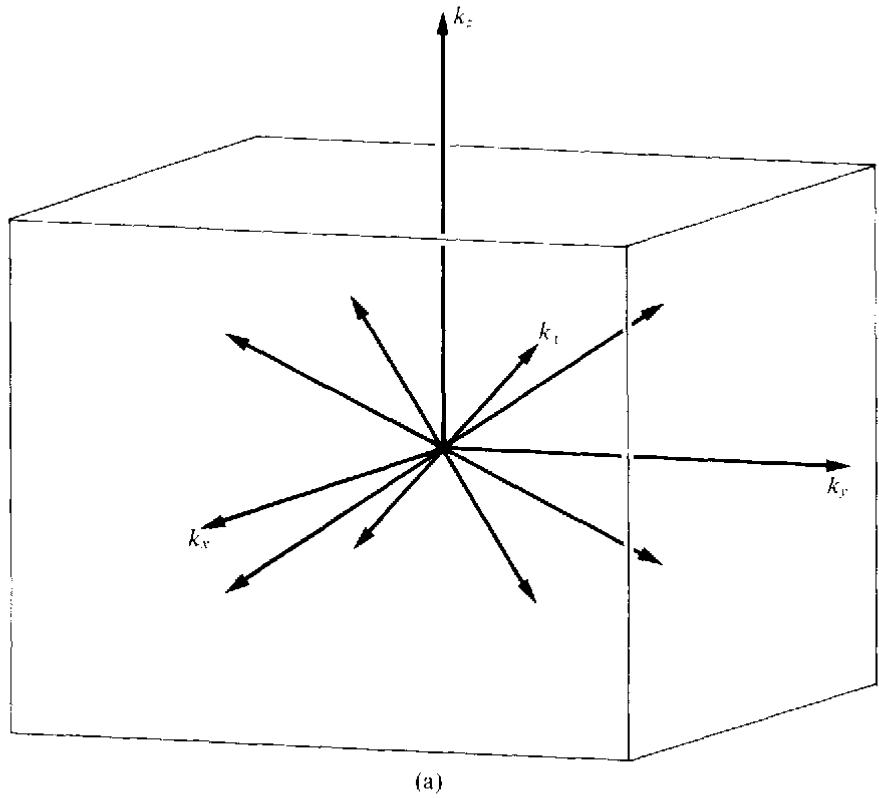
\includegraphics[width=0.75\textwidth]{fig3_19a_mu.jpg}
\caption*{\textbf{图 3.19(a)}\ 布里渊区与确定一个空间群表示的星的矢量。}
\end{figure}
\begin{figure}[H]
\centering
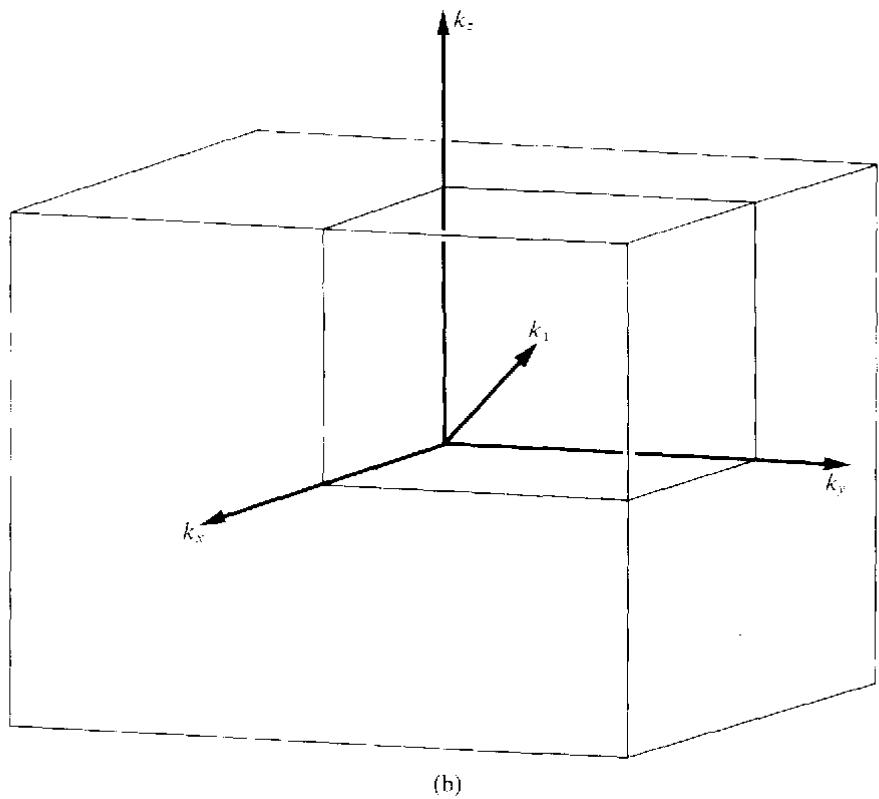
\includegraphics[width=0.75\textwidth]{fig3_19b_mu.jpg}
\caption*{\textbf{图 3.19(b)}\ 表示域与确定一个小表示的矢量。}
\end{figure}

在物理处理中人们会说：在 $\mathbf{k}_{1}$ 处有一组属于 $\Gamma^{\mathbf{k}_{1}}_{p}$ 的 $t$ 个简并本征函数（本征值 $\lambda_{1}$），并且在 $\mathbf{k}_{1}$ 的星中其他每个波矢 $S\mathbf{k}_{1}$ 处也有一组类似的 $t$ 个简并本征函数（本征值相同为 $\lambda_{1}$）。然而由于星的这些其他成员都在表示域之外，而且人们通常只关心本征值的数值（在各表示域中相同），所以只考虑 $\mathbf{k}_{1}$ 处的 $t$ 个本征函数及 $t$ 重简并的本征值。在更严格的数学处理中，则有一组 $(qt)$ 个本征函数具有本征值 $\lambda_{1}$，其中每组 $t$ 个函数与 $\mathbf{k}_{1}$ 的星中的每个波矢相联系。也就是说，$\mathbf{G}$ 的一个表示涉及 $\mathbf{k}_{1}$ 的星中的全部波矢，因此使用 $\mathbf{G}$ 的表示就要用到整个布里渊区，见图 3.19(a)。而小群 $\mathbf{G}^{\mathbf{k}_{1}}$ 的（小）表示只与表示域中的单个波矢 $\mathbf{k}_{1}$ 相联系，见图 3.19(b)。

给出了求 $\mathbf{G}$ 表示的方案之后，现在考虑它在实践中的运作。关键步骤是小表示的确定，方案的其余部分是直截了当的。这里遇到一个基本困难：群 $\mathbf{G}^{\mathbf{k}_{1}}$ 本身是一个空间群！看起来我们几乎回到了出发点。不过 $\mathbf{G}^{\mathbf{k}_{1}}$ 关于 $\mathbf{T}$ 的商群的阶 $b$ 比 $\mathbf{G}/\mathbf{T}$ 的阶 $h$ 小，因此问题有所简化。设
\begin{equation*}
\mathbf{G}^{\mathbf{k}_{1}} = \{S_{1} \mid \mathbf{w}_{1}\}\mathbf{T} + \{S_{2} \mid \mathbf{w}_{2}\}\mathbf{T} + \dots + \{S_{b} \mid \mathbf{w}_{b}\}\mathbf{T},
\tag{3.7.5}
\end{equation*}
并设
\begin{equation*}
\{S_{i} \mid \mathbf{w}_{i}\}\{S_{j} \mid \mathbf{w}_{j}\} = \{S_{i}S_{j} \mid \mathbf{w}_{i} + S_{i}\mathbf{w}_{j}\} = \{E \mid \mathbf{t}_{ij}\}\{S_{k} \mid \mathbf{w}_{k}\},
\tag{3.7.6}
\end{equation*}
其中 $\{E \mid \mathbf{t}_{ij}\} \in \mathbf{T}$，且由式 (3.7.6)
\begin{equation*}
\mathbf{t}_{ij} = \mathbf{w}_{i} + S_{i}\mathbf{w}_{j} - \mathbf{w}_{k}.
\tag{3.7.7}
\end{equation*}
因为 $\mathbf{t}_{ij}$ 是平移，所以
\begin{equation*}
\Gamma^{\mathbf{k}_{1}}_{p}\left(\{S_{i} \mid \mathbf{w}_{i}\}\right)\Gamma^{\mathbf{k}_{1}}_{p}\left(\{S_{j} \mid \mathbf{w}_{j}\}\right) = \exp\left(-\mathrm{i}\mathbf{k}_{1} \cdot (\mathbf{w}_{i} + S_{i}\mathbf{w}_{j} - \mathbf{w}_{k})\right)\Gamma^{\mathbf{k}_{1}}_{p}\left(\{S_{k} \mid \mathbf{w}_{k}\}\right).
\tag{3.7.8}
\end{equation*}
现在若对所有 $\{R \mid \mathbf{v}\} \in \mathbf{G}^{\mathbf{k}_{1}}$ 令
\begin{equation*}
\Gamma^{\mathbf{k}_{1}}_{p}(\{R \mid \mathbf{v}\}) = \exp(-\mathrm{i}\mathbf{k}_{1} \cdot \mathbf{v})\mathbf{D}^{\mathbf{k}_{1}}_{p}(\{R \mid \mathbf{v}\})
\tag{3.7.9}
\end{equation*}
则由式 (3.7.8) 得
\begin{equation*}
\mathbf{D}^{\mathbf{k}_{1}}_{p}\left(\{S_{i} \mid \mathbf{w}_{i}\}\right)\mathbf{D}^{\mathbf{k}_{1}}_{p}\left(\{S_{j} \mid \mathbf{w}_{j}\}\right) = \exp(-\mathrm{i}\mathbf{g}_{i} \cdot \mathbf{w}_{j})\mathbf{D}^{\mathbf{k}_{1}}_{p}\left(\{S_{k} \mid \mathbf{w}_{k}\}\right)
\tag{3.7.10}
\end{equation*}
其中，注意到 $S_{i}\mathbf{k}_{1} \equiv \mathbf{k}_{1}$，$\mathbf{g}_{i}$ 是由方程
\begin{equation*}
S^{-1}_{i}\mathbf{k}_{1} = \mathbf{k}_{1} + \mathbf{g}_{i}
\tag{3.7.11}
\end{equation*}
定义的倒格子矢量。另外，若 $\{E \mid \mathbf{t}\} \in \mathbf{T}$，则由式 (3.7.9)
\begin{equation*}
\mathbf{D}^{\mathbf{k}_{1}}_{p}(\{E \mid \mathbf{t}\}) = 1.
\tag{3.7.12}
\end{equation*}
同样正确的是：若 $\{E \mid \mathbf{t}\} \in \mathbf{T}$，则
\begin{equation*}
\exp\left\{-\mathrm{i}\mathbf{g}_{i} \cdot (\mathbf{w}_{j} + \mathbf{t})\right\} = \exp(-\mathrm{i}\mathbf{g}_{i} \cdot \mathbf{w}_{j}).
\tag{3.7.13}
\end{equation*}
式 (3.7.12)、(3.7.13) 与 (3.7.10) 合起来意味着：$\mathbf{D}^{\mathbf{k}_{1}}_{p}$ 的矩阵对式 (3.7.5) 中任一固定陪集的所有成员都是相同的。也就是说，$\mathbf{D}^{\mathbf{k}_{1}}_{p}$ 是定义在商群 $\mathbf{G}^{\mathbf{k}_{1}}/\mathbf{T}$ 的元素上的矩阵值函数。但这个商群同构于小陪群 $\overline{\mathbf{G}}^{\mathbf{k}_{1}}$。

因此可以把式 (3.7.10) 改写为
\begin{equation*}
\mathbf{D}^{\mathbf{k}_{1}}_{p}(S_{i})\mathbf{D}^{\mathbf{k}_{1}}_{p}(S_{j}) = \exp(-\mathrm{i}\mathbf{g}_{i} \cdot \mathbf{w}_{j})\mathbf{D}^{\mathbf{k}_{1}}_{p}(S_{k}),
\tag{3.7.14}
\end{equation*}
其中 $S_{i}S_{j} = S_{k}$ 且 $S^{-1}_{i}\mathbf{k}_{1} = \mathbf{k}_{1} + \mathbf{g}_{i}$。

由式 (3.7.14) 可见，在如下两种重要情形中 $\mathbf{D}^{\mathbf{k}_{1}}_{p}$ 是 $\overline{\mathbf{G}}^{\mathbf{k}_{1}}$ 到一组矩阵的同态：

（i）若对所有 $j = 1$ 到 $b$ 有 $\mathbf{w}_{j} = 0$。这是空间群 $\mathbf{G}$ 为点式群的情形。

（ii）若对所有 $i = 1$ 到 $b$ 有 $S^{-1}_{i}\mathbf{k}_{1} = \mathbf{k}_{1}$（即 $\mathbf{g}_{i} = 0$）。这是 $\mathbf{k}_{1}$ 为布里渊区内点的情形，因为此时布里渊区中与 $\mathbf{k}_{1}$ 等价的点只有 $\mathbf{k}_{1}$ 自己。

当 $\mathbf{D}^{\mathbf{k}_{1}}_{p}$ 是同态时，它是小陪群的一个表示，而且 $\Gamma^{\mathbf{k}_{1}}_{p}$ 的不可约性意味着 $\mathbf{D}^{\mathbf{k}_{1}}_{p}$ 也必不可约。因此在上述两种情形中，我们要做的只是求出小陪群 $\overline{\mathbf{G}}^{\mathbf{k}_{1}}$ 的不可约表示——这可以从表 2.2 与 2.3 读出。

剩下的唯一情形是 $\mathbf{k}_{1}$ 位于布里渊区面上而空间群为非点式群的情形。

若 $\mathbf{k}_{1}$ 是一般点，则小陪群仅由恒等元构成，又回到情形 (ii)。于是仅有的困难情形是：非点式空间群且 $\mathbf{k}_{1}$ 是对称点，或者 $\mathbf{k}_{1}$ 位于布里渊区面上的对称线或对称面上。

为了覆盖这些困难情形，需要引入有限群的\textit{射影表示}（projective representation）概念。

\noindent\textbf{定义 3.7.5}\quad （射影表示）\ 定义在群 $\mathbf{H}$（由元素 $H_{i}$，$i = 1$ 到 $|\mathbf{H}|$ 组成）上的非奇异矩阵值函数 $\Delta$ 称为 $\mathbf{H}$ 的射影表示，若它满足如下规则：

若对每个群乘积 $H_{i}H_{j} = H_{k}$，存在有序对 $H_{i}, H_{j}$ 上的标量函数 $\mu(H_{i}, H_{j})$ 使得
\begin{equation*}
\Delta(H_{i})\Delta(H_{j}) = \mu(H_{i}, H_{j})\Delta(H_{k})
\tag{3.7.15}
\end{equation*}
并且对一切 $i, j, l$ 有
\begin{equation*}
\mu(H_{i}, H_{j}H_{l})\mu(H_{j}, H_{l}) = \mu(H_{i}H_{j}, H_{l})\mu(H_{i}, H_{j}),
\tag{3.7.16}
\end{equation*}
则称 $\Delta$ 为 $\mathbf{H}$ 的射影表示。式 (3.7.16) 是矩阵乘法结合律的要求。

函数 $\mu(H_{i}, H_{j})$ 构成所谓的射影表示 $\Delta$ 的\textit{因子系统}（factor system）。若对所有 $i, j$ 有 $\mu(H_{i}, H_{j}) = 1$，则射影表示 $\Delta$ 成为普通（矢量）表示。若对所有 $i, j$ 有 $|\mu(H_{i}, H_{j})| = 1$，则总可以施行一个变换使 $\Delta$ 幺正化。幺正射影表示满足与式 (1.3.11) 类似的正交关系：
\begin{equation*}
\sum^{|H|}_{j=1}\Delta^{i}(H_{j})^{*}_{pv}\Delta^{k}(H_{j})_{qw} = \frac{|\mathbf{H}|}{d_{i}}\delta^{ik}\delta_{pq}\delta_{vw},
\tag{3.7.17}
\end{equation*}
相应地，对特征标有
\begin{equation*}
\sum^{|H|}_{j=1}\chi^{i*}(H_{j})\chi^{k}(H_{j}) = |\mathbf{H}|\delta^{ik}.
\tag{3.7.18}
\end{equation*}
给定带因子系统 $\mu$ 的射影表示 $\Delta$，若令
\begin{equation*}
\Delta'(H_{i}) = C_{i}\Delta(H_{i}) \quad\text{对一切 } i,
\tag{3.7.19}
\end{equation*}
其中 $C_{i}$ 是复数，则与式 (3.7.15) 相应的方程为
\begin{equation*}
\Delta'(H_{i})\Delta'(H_{j}) = \frac{C_{i}C_{j}}{C_{k}}\mu(H_{i}, H_{j})\Delta'(H_{k}).
\tag{3.7.20}
\end{equation*}
若再写
\begin{equation*}
\nu(H_{i}, H_{j}) = \frac{C_{i}C_{j}}{C_{k}}\mu(H_{i}, H_{j})
\tag{3.7.21}
\end{equation*}
则 $\Delta'$ 是 $\mathbf{H}$ 的带因子系统 $\nu$ 的射影表示。凡由形如 (3.7.21) 的方程相联系的两个因子系统称为属于同一个\textit{类}。由于关系 (3.7.19) 很简单，我们只需从每个类中选一个因子系统来研究。为从特定类中选取合适的因子系统，注意到
\begin{equation*}
\Delta(E) = \mu(E, E)\mathbf{1}
\tag{3.7.22}
\end{equation*}
若对所有 $i$ 令 $\Delta'(H_{i}) = \Delta(H_{i})/\mu(E, E)$，则
\begin{equation*}
\Delta'(E) = 1.
\tag{3.7.23}
\end{equation*}
再由式 (3.7.21) 定义新的因子系统 $\nu$，取 $1/C_{i} = \mu(E, E)$ 对一切 $i$ 成立，则因为
\begin{equation*}
\Delta'(H_{i})\Delta'(E) = \nu(H_{i}, E)\Delta'(H_{i})
\end{equation*}
必须有
\begin{equation*}
\nu(H_{i}, E) = 1 \quad\text{对一切 } H_{i}.
\tag{3.7.24}
\end{equation*}
类似地
\begin{equation*}
\nu(E, H_{i}) = 1 \quad\text{对一切 } H_{i}.
\tag{3.7.25}
\end{equation*}
（对任何因子系统 $\mu$，当然有 $\mu(H_{i}, E) = \mu(E, H_{i}) = \mu(E, E)$，以及 $\mu(H_{i}, H^{-1}_{i}) = \mu(H^{-1}_{i}, H_{i})$。）

现在不加证明地引用 Schur 关于射影表示的若干定理。

\noindent\textbf{定理 3.7.1}\quad 有限群 $\mathbf{H}$ 的因子系统的类数 $m$ 是有限的；这些类可以与一个 $m$ 阶 Abel 群 $\mathbf{M}$（称为 $\mathbf{H}$ 的\textit{乘子}（multiplier））的元素一一对应。

这一对应是这样的：若把 $\mathbf{M}$ 的元素记为 $M_{1}, M_{2}, \dots, M_{m}$，而 $\mu_{p}$、$\mu_{q}$ 是从分别对应于 $M_{p}$ 与 $M_{q}$ 的类中任取的因子系统，则对一切 $i, j$ 由
\begin{equation*}
\mu_{r}(H_{i}, H_{j}) = \mu_{p}(H_{i}, H_{j})\mu_{q}(H_{i}, H_{j})
\tag{3.7.26}
\end{equation*}
定义的因子系统 $\mu_{r}$ 总属于对应于 $M_{r}$ 的类，其中 $M_{r} = M_{p}M_{q}$。此外，$\mathbf{M}$ 的每个元素的阶都整除 $|\mathbf{H}|$。特别地，若 $M_{p}$ 的阶为 $\alpha_{p}$，则可以从对应于 $M_{p}$ 的类中选出一个代表因子系统，其取值全是单位根的 $\alpha_{p}$ 次幂。

Schur 的理论进而证明：对每个 $|\mathbf{H}|$ 阶、乘子 $\mathbf{M}$ 为 $m$ 阶的有限群 $\mathbf{H}$，可以构造一个 $|\mathbf{H}|m$ 阶的群 $\mathbf{H}_{M}$，使 $\mathbf{M}$ 同构于 $\mathbf{H}_{M}$ 中心的一个子群（群的中心是与所有元素可交换的不变子群）。

\noindent\textbf{定理 3.7.2}\quad 通过遍取 $\mathbf{H}_{M}$ 的所有表示并限制在 $\mathbf{H}$ 的元素上，可以（在等价意义下）得到 $\mathbf{H}$ 的全部可能的幺正不可约射影表示。

联系这个定理必须意识到：尽管 $\mathbf{H}$ 的元素可以被认作 $\mathbf{H}_{M}/\mathbf{M}$ 的陪集代表，$\mathbf{H}_{M}$ 的构造方式使得除平凡情形 $m = 1$ 外，$\mathbf{H}_{M}$ 中被认定为 $\mathbf{H}$ 元素的那些元素的乘法规则与 $\mathbf{H}$ 中的乘法规则不同。

由于这个定理比我们需要的更强，我们将不说明如何构造 $\mathbf{H}_{M}$。记住我们只要求属于给定因子系统的射影表示。我们将不构造 $\mathbf{H}_{M}$，而是说明如何构造另一个群 $\mathbf{H}^{*}$，它给出的是属于给定因子系统的全部不可约射影表示（而不是所有因子系统的）。

设我们有一个群 $\mathbf{H}$，希望求出它属于给定因子系统 $\mu$ 的幺正不可约射影表示。由目前的讨论可知，可以把 $\mu$ 选成对一切 $j, k$ 有
\begin{equation*}
\mu(H_{j}, H_{k}) = \exp\left\{2\pi\mathrm{i}\,a(H_{j}, H_{k})/g\right\},
\tag{3.7.27}
\end{equation*}
其中 $g$ 与 $a(H_{j}, H_{k})$ 是由已知的 $\mu(H_{j}, H_{k})$ 及条件 $0 \leqslant a(H_{j}, H_{k}) \leqslant g-1$ 确定的整数，并且（见式 (3.7.24) 与 (3.7.25)）
\begin{equation*}
a(H_{j}, E) = a(E, H_{j}) = 0.
\tag{3.7.28}
\end{equation*}
另外，由于 $\mu(H_{j}, H^{-1}_{j}) = \mu(H^{-1}_{j}, H_{j})$，
\begin{equation*}
a(H_{j}, H^{-1}_{j}) = a(H^{-1}_{j}, H_{j})
\tag{3.7.29}
\end{equation*}
且由式 (3.7.16) 与 (3.7.27)，
\begin{equation*}
a(H_{i}, H_{j}H_{l}) + a(H_{j}, H_{l}) = a(H_{i}H_{j}, H_{l}) + a(H_{i}, H_{j}), \mod g.
\tag{3.7.30}
\end{equation*}
设 $\mathbf{Z}_{g}$ 是整数 $0, 1, \dots, (g-1)$ 的循环群，群乘法定义为模 $g$ 加法。

设 $\mathbf{H}^{*}$ 由 $g|\mathbf{H}|$ 个元素（即一对一对的 $(H_{j}, \alpha)$，其一来自 $\mathbf{H}$，另一来自 $\mathbf{Z}_{g}$）组成，并用方程
\begin{equation*}
(H_{j}, \alpha)(H_{k}, \beta) = (H_{j}H_{k}, \alpha + \beta + a(H_{j}, H_{k}))
\tag{3.7.31}
\end{equation*}
定义乘法规则。关于这一乘法规则 $\mathbf{H}^{*}$ 是群：封闭性显然；结合性由 $\mathbf{H}$ 与 $\mathbf{Z}_{g}$ 中的结合性及式 (3.7.30) 得到；$\mathbf{H}^{*}$ 的恒等元是 $(E, 0)$；$(H_{j}, \alpha)$ 的逆是 $(H^{-1}_{j}, -\alpha - a(H^{-1}_{j}, H_{j}))$。

由式 (3.7.31) 与 (3.7.28) 可知，对一切 $\alpha, \beta, k$ 有
\begin{equation*}
(E, \alpha)(H_{k}, \beta) = (H_{k}, \beta)(E, \alpha) = (H_{k}, \alpha + \beta).
\tag{3.7.32}
\end{equation*}
式 (3.7.32) 蕴含由 $g$ 个元素 $(E, \alpha)$ 组成的子群位于 $\mathbf{H}^{*}$ 的中心。既然 $(E, \alpha)$ 与 $\mathbf{H}^{*}$ 的所有元素可交换，由 Schur 引理（见定理 1.3.6）可知，若 $\Gamma$ 是 $\mathbf{H}^{*}$ 的表示，则 $\Gamma(E, \alpha)$ 是单位矩阵的标量倍。

现在假设存在 $\mathbf{H}^{*}$ 的一个表示使得对一切 $\alpha \in \mathbf{Z}_{g}$ 有
\begin{equation*}
\Gamma(E, \alpha) = \exp(2\pi\mathrm{i}\alpha/g)\mathbf{1}.
\tag{3.7.33}
\end{equation*}
则
\begin{equation*}
\Gamma(H_{k}, \beta) = \Gamma(H_{k}, 0)\Gamma(E, \beta) = \Gamma(H_{k}, 0)\exp(2\pi\mathrm{i}\beta/g)
\tag{3.7.34}
\end{equation*}
记 $\Gamma(H_{k}, 0) = \Delta(H_{k})$，便有
\begin{equation*}
\begin{aligned}
\Delta(H_{j})\Delta(H_{k}) &= \Gamma(H_{j}, \alpha)\Gamma(H_{k}, \beta)\exp\left\{-2\pi\mathrm{i}(\alpha + \beta)/g\right\}\\
&= \Gamma(H_{j}H_{k}, \alpha + \beta + a(H_{j}, H_{k}))\exp\left\{-2\pi\mathrm{i}(\alpha + \beta)/g\right\}\\
&= \Delta(H_{j}H_{k})\exp\left\{2\pi\mathrm{i}\,a(H_{j}, H_{k})/g\right\}.
\end{aligned}
\tag{3.7.35}
\end{equation*}
由式 (3.7.35) 与 (3.7.27) 可知 $\Delta$ 是 $\mathbf{H}$ 的带因子系统 $\mu$ 的射影表示。而且它是幺正的（因为 $\Gamma$ 幺正），也是不可约的（因为若 $\Delta$ 可约，则由于 $(E, \alpha)$ 对一切 $\alpha$ 由标量矩阵表示，$\Gamma$ 的所有矩阵就都与 $\Delta$ 的矩阵处于同样的分块对角形式，与 $\Gamma$ 的不可约性矛盾）。

反之，若 $\Delta$ 是 $\mathbf{H}$ 的幺正不可约射影表示，且对一切 $k, \beta$ 令
\begin{equation*}
\Gamma(H_{k}, \beta) = \Delta(H_{k})\exp(2\pi\mathrm{i}\beta/g)
\tag{3.7.36}
\end{equation*}
则 $\Gamma$ 是 $\mathbf{H}^{*}$ 的表示。于是用纯数学家的语言说，$\mathbf{H}$ 的全部不可约射影表示都可以提升到 $\mathbf{H}^{*}$ 中，也就是说可以由 $\mathbf{H}^{*}$ 的普通矢量表示求得。

现在回到小陪群，考察我们关心的因子系统。把 $\overline{\mathbf{G}}^{\mathbf{k}_{1}}$ 认同于 $\mathbf{H}$，把 $\mathbf{D}^{\mathbf{k}_{1}}_{p}$ 认同于 $\Delta$。因子系统由下式给出：
\begin{equation*}
\mu(S_{i}, S_{j}) = \exp(-\mathrm{i}\mathbf{g}_{i} \cdot \mathbf{w}_{j})
\tag{3.7.37}
\end{equation*}
其中
\begin{equation*}
S^{-1}_{i}\mathbf{k}_{1} = \mathbf{k}_{1} + \mathbf{g}_{i}
\tag{3.7.11}
\end{equation*}
而 $\mathbf{w}_{j}$ 是在 $\mathbf{G}^{\mathbf{k}_{1}}$ 关于 $\mathbf{T}$ 的左陪集分解 (3.7.5) 中与 $S_{j}$ 相联系的平移部分。

由式 (3.7.11) 可见，当 $S_{i} = E$ 时 $\mathbf{g}_{i} = 0$，故
\begin{equation*}
\mu(E, S_{j}) = 1 \quad\text{对一切 } j.
\end{equation*}
此外，由于 $\mathbf{w}_{j}$ 总是平移的分数部分，$\mu(S_{j}, S_{k})$ 总具有 (3.7.27) 的形式；更重要的是，$g$ 必然是个小数目（事实上是 2、3、4 或 6）。于是由式 (3.7.37) 定义的因子系统已经处于适于上述处理的形式。这意味着，为求出空间群的所有表示，只需找出几个小群（的中央延拓群）的普通表示就够了。

作为本节的最后一点，通过分析 $\mathbf{H}_{M}$ 的表示的维数，并注意其中哪些对给定因子系统成为不可约幺正射影表示，可以证明一个与定理 1.3.11 类似的定理：若给定因子系统的射影表示的维数为 $d_{i}$，则 $\sum_{i}d^{2}_{i} = |\mathbf{H}|$。这使式 (3.7.17) 可以反过来产生另一个矩阵元的正交关系。但要注意，$i$ 的取值个数不一定等于 $\mathbf{H}$ 的类的数目（这与普通矢量表示不同）。

% 3.8 例子：立方密堆积与金刚石结构
\section{例子：立方密堆积与金刚石结构}

本节给出两个例子来说明前几节的理论；一个是点式空间群——立方密堆积 $Fm3m\ (O^{5}_{h})$，另一个是非点式空间群——金刚石结构的空间群 $Fd3m\ (O^{7}_{h})$。这两个空间群分别最先由 Bouckaert, Smoluchowski, and Wigner (1936) 与 Herring (1942) 处理过。

二者都建立在面心立方（$F$）布拉维格子 $\Gamma^{f}_{c}$ 上，故由表 3.1，两种情形的格子平移都是
\begin{equation*}
\left\{
\begin{array}{l}
\mathbf{t}_{1} = \frac{1}{2}(0, a, a),\\
\mathbf{t}_{2} = \frac{1}{2}(a, 0, a),\\
\mathbf{t}_{3} = \frac{1}{2}(a, a, 0).
\end{array}
\right.
\tag{3.8.1}
\end{equation*}
两种情形的同形点群 $\mathbf{F}$ 都是 $m3m\ (O_{h})$，即完整立方群。

由表 3.3 可见倒格子矢量为
\begin{equation*}
\left\{
\begin{array}{l}
\mathbf{g}_{1} = (2\pi/a)(-1, 1, 1),\\
\mathbf{g}_{2} = (2\pi/a)(1, -1, 1),\\
\mathbf{g}_{3} = (2\pi/a)(1, 1, -1),
\end{array}
\right.
\tag{3.8.2}
\end{equation*}
布里渊区示于图 3.14。

由表 3.7 可见，对 $Fm3m\ (O^{5}_{h})$，$m3m\ (O_{h})$ 的每个转动算符都只与纯格子平移相联系，于是关于平移群 $\mathbf{T}$ 的一个合适的左陪集分解为
\begin{equation*}
Fm3m\left(O^{5}_{h}\right) = \sum_{R}\{R \mid 000\}\mathbf{T}
\tag{3.8.3}
\end{equation*}
其中对 $R$ 的求和取遍 $m3m\ (O_{h})$ 的所有元素。而对 $Fd3m\ (O^{7}_{h})$，只有属于子群 $\bar{4}3m\ (T_{d})$ 的算符与纯格子平移相联系，相应的左陪集分解为
\begin{equation*}
Fd3m\left(O^{7}_{h}\right) = \sum_{R}\{R \mid 000\}\mathbf{T} + \sum_{R}\{RI \mid {\textstyle\frac{1}{4}}{\textstyle\frac{1}{4}}{\textstyle\frac{1}{4}}\}\mathbf{T}
\tag{3.8.4}
\end{equation*}
此时对 $R$ 的求和取遍 $\bar{4}3m\ (T_{d})$ 的所有元素，且如通常，$I$ 是反演。与不在 $\bar{4}3m\ (T_{d})$ 中的 $m3m\ (O_{h})$ 元素相对应的那些陪集，其陪集代表总可取为 $\mathbf{v} = \frac{1}{4}(\mathbf{t}_{1} + \mathbf{t}_{2} + \mathbf{t}_{3}) = \frac{1}{4}(a, a, a)$（在 $Oxyz$ 轴下）。算符 $R$ 作用在（$Oxyz$ 轴下的）非零平移 $(p, q, r)$ 上的效果可由表 1.4 查出，例如 $C^{-}_{4z}(p, q, r) = (q, -p, r)$。算符 $R$ 作用在布拉维格子基本矢量 $\mathbf{t}_{1}$、$\mathbf{t}_{2}$、$\mathbf{t}_{3}$ 上的效果可由表 3.2 查出，例如对立方 $F$ 格子 $C^{-}_{4z}\mathbf{t}_{1} = \mathbf{t}_{2}$、$C^{-}_{4z}\mathbf{t}_{2} = \mathbf{t}_{2} - \mathbf{t}_{3}$、$C^{-}_{4z}\mathbf{t}_{3} = -\mathbf{t}_{1} + \mathbf{t}_{2}$。

在表 3.11 中我们列出了布里渊区基本域中我们求 $Fm3m\ (O^{5}_{h})$ 与 $Fd3m\ (O^{7}_{h})$ 的表示时所需要的对称点、对称线和对称面以及一个一般点。它们就是 3.7 节的点 $\mathbf{k}_{1}$。两种情形下，由于 $\mathbf{F}$ 是布拉维格子的全对称点群，表示域与基本域重合，因此就是图 3.14 所示的区域。

\begin{figure}[H]
\centering
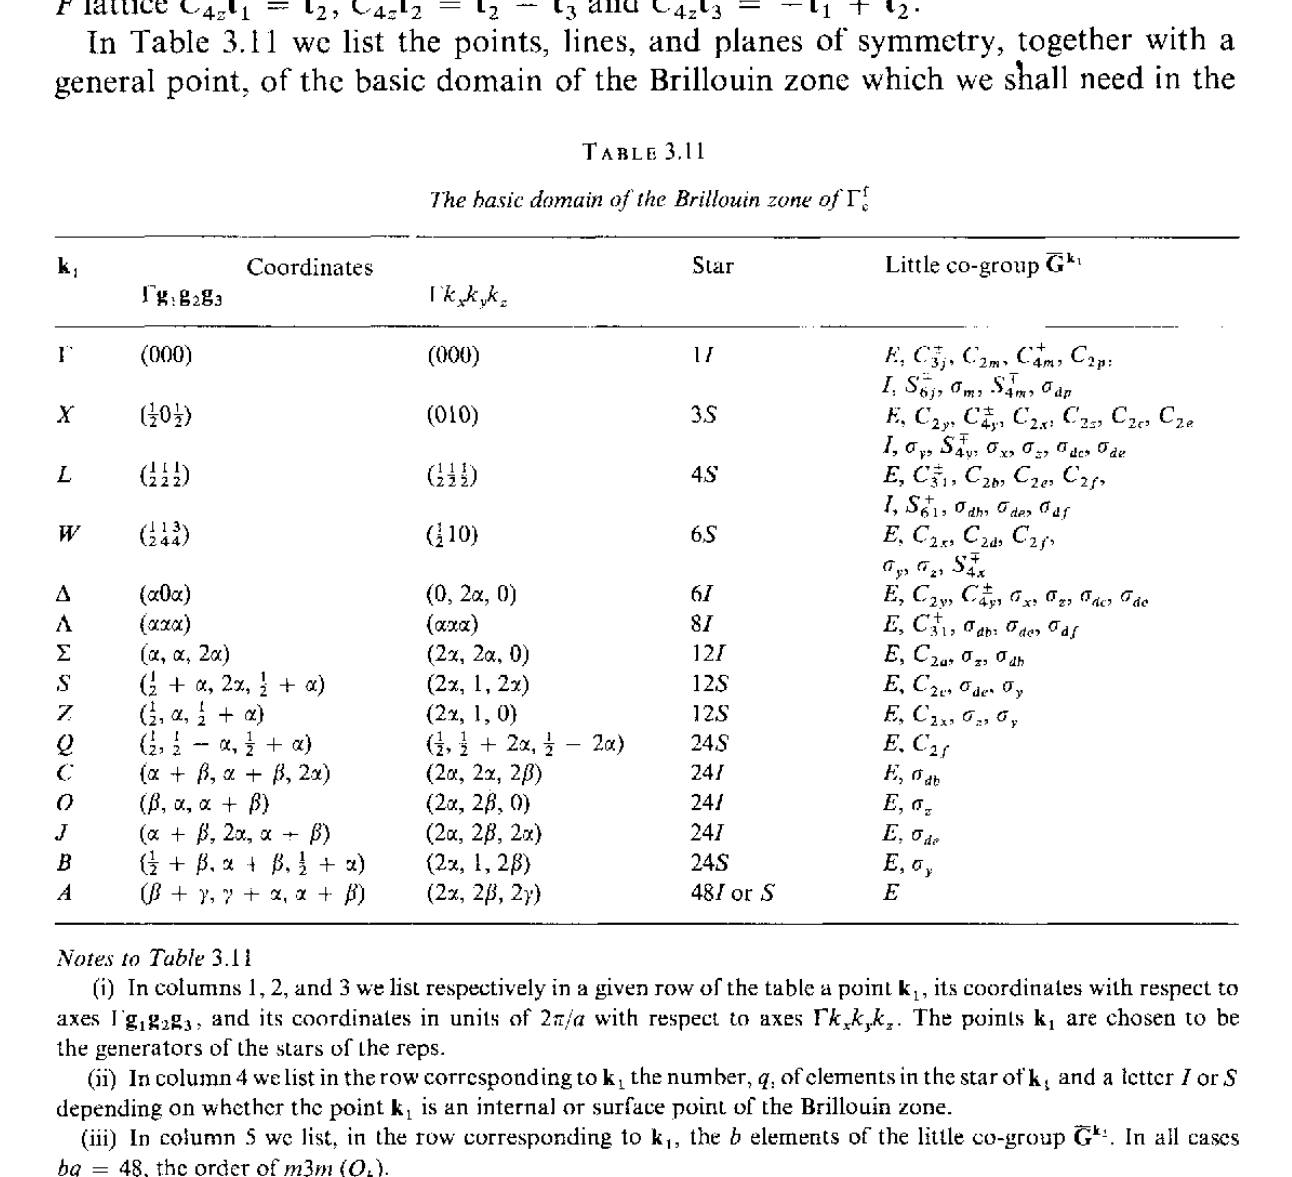
\includegraphics[width=0.88\textwidth]{c3_t311.png}
\caption*{\textbf{表 3.11}\ $\Gamma^{f}_{c}$ 的布里渊区的基本域（原书扫描占位）。}
\end{figure}

表 3.11 的注（译文）：

\noindent（i）第 1、2、3 列在表的每一行中分别列出点 $\mathbf{k}_{1}$、它相对于轴 $\Gamma\mathbf{g}_{1}\mathbf{g}_{2}\mathbf{g}_{3}$ 的坐标，以及它以 $2\pi/a$ 为单位、相对于轴 $\Gamma k_{x}k_{y}k_{z}$ 的坐标。点 $\mathbf{k}_{1}$ 选为表示的星的生成元。

\noindent（ii）第 4 列在对应于 $\mathbf{k}_{1}$ 的行中列出 $\mathbf{k}_{1}$ 的星中元素的数目 $q$，以及字母 I 或 S——视 $\mathbf{k}_{1}$ 是布里渊区的内部点还是表面点而定。

\noindent（iii）第 5 列在对应于 $\mathbf{k}_{1}$ 的行中列出小陪群 $\overline{\mathbf{G}}^{\mathbf{k}_{1}}$ 的 $b$ 个元素。所有情形都有 $bq = 48$，即 $m3m\ (O_{h})$ 的阶。

\noindent（iv）本表对两个空间群乃至一切基于 $\Gamma^{f}_{c}$ 且同形点群为 $m3m\ (O_{h})$ 的空间群都是共同的；另见表 3.6 的相应部分。表 3.11 中有而表 3.6 中没有的点，是对称面上的点与一般点。除本例外我们将不再列出对称面，因为如我们将看到的，它们很容易处理。

现在考虑把小群 $\mathbf{G}^{\mathbf{k}_{1}}$ 关于平移群 $\mathbf{T}$ 作左陪集分解。对 $Fm3m$ 有
\begin{equation*}
\mathbf{G}^{\mathbf{k}_{1}} = \sum_{S}\{S \mid 000\}\mathbf{T}
\tag{3.8.5}
\end{equation*}
其中对 $S$ 的求和取遍 $\overline{\mathbf{G}}^{\mathbf{k}_{1}}$ 的所有元素（这些群见表 3.11）。而对 $Fd3m$ 有
\begin{equation*}
\mathbf{G}^{\mathbf{k}_{1}} = \sum_{P}\{P \mid 000\}\mathbf{T} + \sum_{Q}\{Q \mid {\textstyle\frac{1}{4}}{\textstyle\frac{1}{4}}{\textstyle\frac{1}{4}}\}\mathbf{T},
\tag{3.8.6}
\end{equation*}
其中对 $P$ 的求和取遍 $\overline{\mathbf{G}}^{\mathbf{k}_{1}}$ 与 $\bar{4}3m\ (T_{d})$ 共有的元素，对 $Q$ 的求和取遍 $\overline{\mathbf{G}}^{\mathbf{k}_{1}}$ 的其余元素。

\subsection*{Fm3m}

$Fm3m$ 可以很快处理完。给定任一点 $\mathbf{k}_{1}$，需要确定 $\overline{\mathbf{G}}^{\mathbf{k}_{1}}$ 带因子系统 $\exp(-\mathrm{i}\mathbf{g}_{i} \cdot \mathbf{w}_{j})$ 的射影表示，其中 $\mathbf{g}_{i}$ 由式 (3.7.11) 给出，$\mathbf{w}_{j}$ 是分解 (3.8.5) 中与 $S_{j}$ 相联系的平移。立即看出对所有 $j$ 有 $\mathbf{w}_{j} = 0$。因此因子系统完全由单位元组成，属于 $\overline{\mathbf{G}}^{\mathbf{k}_{1}}$ 的乘子的恒等元所对应的类。于是合适的表示 $\mathbf{D}^{\mathbf{k}_{1}}_{p}$ 就是 $\overline{\mathbf{G}}^{\mathbf{k}_{1}}$ 的普通矢量表示；而且由于 $\overline{\mathbf{G}}^{\mathbf{k}_{1}}$ 是点群（诚然某些情形下定向非标准），可以从表 2.2 得到 $\mathbf{D}^{\mathbf{k}_{1}}_{p}$。

$\mathbf{G}^{\mathbf{k}_{1}}$ 的小表示 $\Gamma^{\mathbf{k}_{1}}_{p}$ 现在由式 (3.7.9) 立即得到。$\Gamma^{\mathbf{k}_{1}}_{p}$ 的矩阵在所有情形都与 $\mathbf{D}^{\mathbf{k}_{1}}_{p}$ 的矩阵通过方程
\begin{equation*}
\Gamma^{\mathbf{k}_{1}}_{p}(\{S \mid \mathbf{t}\}) = \exp(-\mathrm{i}\mathbf{k}_{1} \cdot \mathbf{t})\mathbf{D}^{\mathbf{k}_{1}}_{p}(S)
\tag{3.8.7}
\end{equation*}
相联系。因此只需指明点群 $\overline{\mathbf{G}}^{\mathbf{k}_{1}}$ 即可把 $Fm3m$ 处理完毕。结果如下：对 $\Gamma$，$m3m\ (O_{h})$；对 $X$，$4/mmm\ (D_{4h})$；对 $L$，$\bar{3}m\ (D_{3d})$；对 $W$，$\bar{4}2m\ (D_{2d})$；对 $\Delta$，$4mm\ (C_{4v})$；对 $\Lambda$，$3m\ (C_{3v})$；对 $\Sigma$，$mm2\ (C_{2v})$；对 $S$，$mm2\ (C_{2v})$；对 $Z$，$mm2\ (C_{2v})$；对 $Q$，$2\ (C_{2})$；对 $C$，$m\ (C_{1h})$；对 $O$，$m\ (C_{1h})$；对 $J$，$m\ (C_{1h})$；对 $B$，$m\ (C_{1h})$；对 $A$，$1\ (C_{1})$。

\subsection*{Fd3m}

金刚石的情形就不那么容易了。首先注意到，在分解 (3.8.6) 中，若陪集代表的转动部分 $P$ 是元素 $E$、$C^{\pm}_{3j}$、$C_{2m}$、$\sigma_{dp}$ 或 $S^{\pm}_{4m}$ 之一，则其平移部分 $\mathbf{w}_{j} = 0$；而若其转动部分 $Q$ 是元素 $I$、$S^{\mp}_{6j}$、$\sigma_{m}$、$C_{2p}$ 或 $C^{\pm}_{4m}$ 之一，则其平移部分 $\mathbf{w}_{j} = \mathbf{v} = \frac{1}{4}(a, a, a)$。因此因子系统 $\exp(-\mathrm{i}\mathbf{g}_{i} \cdot \mathbf{w}_{j})$ 在下述两种情形完全由单位元组成：对所有 $i$ 有 $\mathbf{g}_{i} = \mathbf{0}$；或者小陪群 $\overline{\mathbf{G}}^{\mathbf{k}_{1}}$ 的元素全部形如 $P$ 而没有形如 $Q$ 的元素。前者在 $\mathbf{k}_{1}$ 是布里渊区内点时成立（$\Gamma, \Delta, \Lambda, \Sigma, C, O, J, A(\mathrm{I})$），后者在 $\overline{\mathbf{G}}^{\mathbf{k}_{1}}$ 完全由 $\bar{4}3m\ (T_{d})$ 中的元素组成时成立（$\Lambda, C, J, A(\mathrm{S})$）。这些情形所需的射影表示 $\mathbf{D}^{\mathbf{k}_{1}}_{p}$ 就是点群 $\overline{\mathbf{G}}^{\mathbf{k}_{1}}$ 的普通表示。

于是，在 $Fd3m$ 中若 $\mathbf{k}_{1} = \Gamma, \Delta, \Lambda, \Sigma, C, O, J$ 或 $A$，求 $\mathbf{D}^{\mathbf{k}_{1}}_{p}$ 时只需在表 2.2 中查 $\overline{\mathbf{G}}^{\mathbf{k}_{1}}$ 的表示即可。与这些点对应的点群 $\overline{\mathbf{G}}^{\mathbf{k}_{1}}$ 的名称已在上面处理 $Fm3m$ 时给出。然而，即使对这些点，$Fd3m$ 与 $Fm3m$ 之间也有本质差别：得到 $\mathbf{D}^{\mathbf{k}_{1}}_{p}$ 之后，小表示 $\Gamma^{\mathbf{k}_{1}}_{p}$ 的导出方式与 $Fm3m$ 不完全一样。此时由式 (3.7.9) 可见
\begin{equation*}
\Gamma^{\mathbf{k}_{1}}_{p}(\{P \mid \mathbf{t}\}) = \exp(-\mathrm{i}\mathbf{k}_{1} \cdot \mathbf{t})\mathbf{D}^{\mathbf{k}_{1}}_{p}(P),
\tag{3.8.8}
\end{equation*}
但
\begin{equation*}
\Gamma^{\mathbf{k}_{1}}_{p}(\{Q \mid \mathbf{t} + \mathbf{v}\}) = \exp\left(-\mathrm{i}\mathbf{k}_{1} \cdot (\mathbf{t} + \mathbf{v})\right)\mathbf{D}^{\mathbf{k}_{1}}_{p}(Q),
\tag{3.8.9}
\end{equation*}
其中 $P$ 与 $Q$ 的含义与分解 (3.8.6) 中相同。由于习惯上列出的是小表示 $\Gamma^{\mathbf{k}_{1}}_{p}$ 而非 $\mathbf{D}^{\mathbf{k}_{1}}_{p}$，表中出现的某些元素带有一个额外因子 $\exp(-\mathrm{i}\mathbf{k}_{1} \cdot \mathbf{v})$，它不出现在相应点群的特征标表中。（值得指出，对 $\Gamma$ 这个因子总是 1，因此属于 $\Gamma$ 的非点式空间群的表示与相应点式空间群的表示相同。）

现在详细考虑布里渊区的每个表面点 $B, Q, Z, S, L, W$ 和 $X$。我们将不加解释地使用 3.7 节后面各段的记号。

\subsection*{B}

$\mathbf{G}^{B}$ 的陪集代表：$\{E \mid 000\}$，$\{\sigma_{y} \mid {\frac{1}{4}}{\frac{1}{4}}{\frac{1}{4}}\}$。

\begin{center}
$EB = B$，于是 $\mathbf{g}_{E} = 0$。

$\sigma_{y}B = B - \mathbf{g}_{1} - \mathbf{g}_{3}$，于是 $\mathbf{g}_{\sigma_{y}} = -\mathbf{g}_{1} - \mathbf{g}_{3} = (-1, 0, -1)$。
\end{center}

因子系统：$\mu(E, E) = 1$，$\mu(E, \sigma_{y}) = 1$，$\mu(\sigma_{y}, E) = 1$，以及 $\mu(\sigma_{y}, \sigma_{y}) = \exp\left(2\pi\mathrm{i}\left(\frac{1}{4} + 0 + \frac{1}{4}\right)\right) = -1$。

中央延拓群 $\overline{\mathbf{G}}^{B*}$ 由四个元素 $(E, 0)$、$(E, 1)$、$(\sigma_{y}, 0)$、$(\sigma_{y}, 1)$ 组成，乘法表为
\begin{center}
\begin{tabular}{lcccc}
 & $(E, 0)$ & $(E, 1)$ & $(\sigma_{y}, 0)$ & $(\sigma_{y}, 1)$\\
$(E, 1)$ & $(E, 0)$ & $(E, 1)$ & $(\sigma_{y}, 1)$ & $(\sigma_{y}, 0)$\\
$(\sigma_{y}, 0)$ & $(\sigma_{y}, 1)$ & $(\sigma_{y}, 0)$ & $(E, 1)$ & $(E, 0)$\\
$(\sigma_{y}, 1)$ & $(\sigma_{y}, 0)$ & $(\sigma_{y}, 1)$ & $(E, 0)$ & $(E, 1)$
\end{tabular}
\end{center}
由此看出 $\overline{\mathbf{G}}^{B*}$ 同构于 $C_{4}$。我们关心的是 $\overline{\mathbf{G}}^{B*}$ 中满足 $\mathbf{D}(E, 1) = -\mathbf{1}$ 的那些表示（见式 (3.7.33)，取 $\alpha = 1$，$g = 2$）。由表 2.2 可见这是两个一维表示：
\begin{center}
\begin{tabular}{lcccc}
 & $(E, 0)$ & $(\sigma_{y}, 0)$ & $(E, 1)$ & $(\sigma_{y}, 1)$\\
${}^{1}E$ & $1$ & $-i$ & $-1$ & $i$\\
${}^{2}E$ & $1$ & $i$ & $-1$ & $-i$
\end{tabular}
\end{center}
由式 (3.8.8) 与 (3.8.9) 可见，$\mathbf{G}^{B}$ 的小表示的特征标表中相应的项为
\begin{center}
\begin{tabular}{lcc}
$B$ & $\{E \mid 000\}$ & $\{\sigma_{y} \mid \frac{1}{4}\frac{1}{4}\frac{1}{4}\}$\\
${}^{1}E$ & $1$ & $-i\zeta$\\
${}^{2}E$ & $1$ & $i\zeta$
\end{tabular}
\end{center}
其中 $\zeta = \exp(-\mathrm{i}\mathbf{k}_{1} \cdot \mathbf{v})$。

\subsection*{Q}

$\mathbf{G}^{Q}$ 的陪集代表：$\{E \mid 000\}$，$\{C_{2f} \mid {\frac{1}{4}}{\frac{1}{4}}{\frac{1}{4}}\}$。

$EQ = Q$，于是 $\mathbf{g}_{E} = 0$。

$C_{2f}Q = Q - \mathbf{g}_{1} - \mathbf{g}_{2} - \mathbf{g}_{3}$，于是 $\mathbf{g}_{Q} = -(\mathbf{g}_{1} + \mathbf{g}_{2} + \mathbf{g}_{3}) = (-1, -1, -1)$。

因子系统：$\mu(E, E) = 1$，$\mu(E, C_{2f}) = 1$，$\mu(C_{2f}, E) = 1$，以及 $\mu(C_{2f}, C_{2f}) = -i$。

中央延拓群 $\overline{\mathbf{G}}^{Q*}$ 由八个元素组成，同构于 $C_{8}$，使得 $(C_{2f}, 0)^{8} = (E, 0)$ 且 $(C_{2f}, 0)^{6} = (E, 1)$。我们关心的是 $\overline{\mathbf{G}}^{Q*}$ 中满足 $\mathbf{D}(E, 1) = i\mathbf{1}$ 的表示（见式 (3.7.33)，取 $\alpha = 1$，$g = 4$）。这是两个一维表示，其中特征标表的相应项为
\begin{center}
\begin{tabular}{lcc}
 & $(E, 0)$ & $(C_{2f}, 0)$\\
${}^{1}E_{3}$ & $1$ & $\exp(3\pi i/4)$\\
${}^{2}E_{1}$ & $1$ & $\exp(7\pi i/4)$
\end{tabular}
\end{center}
由于 $\exp(-\mathrm{i}\mathbf{k}_{1} \cdot \mathbf{v}) = \exp(-3\pi\mathrm{i}/4)$，可见 $\mathbf{G}^{Q}$ 的小表示的特征标表中相应的项为
\begin{center}
\begin{tabular}{lcc}
$Q$ & $\{E \mid 000\}$ & $\{C_{2f} \mid {\frac{1}{4}}{\frac{1}{4}}{\frac{1}{4}}\}$\\
${}^{1}E_{3}$ & $1$ & $+1$\\
${}^{2}E_{1}$ & $1$ & $-1$
\end{tabular}
\end{center}

\subsection*{Z}

$\mathbf{G}^{Z}$ 的陪集代表：$\{E \mid 000\}$，$\{C_{2x} \mid 000\}$，$\{\sigma_{y} \mid {\frac{1}{4}}{\frac{1}{4}}{\frac{1}{4}}\}$，$\{\sigma_{z} \mid {\frac{1}{4}}{\frac{1}{4}}{\frac{1}{4}}\}$。

\begin{center}
$\mathbf{g}_{E} = 0$，$\mathbf{g}_{C_{2x}} = (-1, 0, -1)$，$\mathbf{g}_{\sigma_{z}} = 0$，$\mathbf{g}_{\sigma_{y}} = (-1, 0, -1)$。
\end{center}

因子系统的元素全部等于 1，除了 $\mu(C_{2x}, \sigma_{z}) = \mu(C_{2x}, \sigma_{y}) = \mu(\sigma_{y}, \sigma_{z}) = \mu(\sigma_{y}, \sigma_{y}) = -1$。

中央延拓群 $\overline{\mathbf{G}}^{Z*}$ 由八个元素组成，同构于 $422\ (D_{4})$，使得 $(\sigma_{y}, 0)^{4} = (\sigma_{z}, 0)^{2} = (E, 0)$ 且 $(\sigma_{z}, 0)(\sigma_{y}, 0) = (\sigma_{y}, 0)^{3}$，$(\sigma_{z}, 0)(\sigma_{y}, 0)^{-1} = (C_{2x}, 0)$。我们关心的是 $\overline{\mathbf{G}}^{Z*}$ 中满足 $\mathbf{D}(E, 1) = -\mathbf{1}$ 的表示；由表 2.2 可见这是表示 $E$，其特征标为
\begin{center}
\begin{tabular}{lccccc}
 & $(E, 0)$ & $(E, 1)$ & $(\sigma_{y}, 0)(\sigma_{y}, 1)$ & $(\sigma_{z}, 0)(\sigma_{z}, 1)$ & $(C_{2x}, 0)(C_{2x}, 1)$\\
$E$ & $2$ & $-2$ & $0$ & $0$ & $0$
\end{tabular}
\end{center}
可能的矩阵为
\begin{equation*}
\mathbf{D}_{E}(E, 0) = \begin{pmatrix} 1 & 0\\ 0 & 1 \end{pmatrix}, \qquad
\mathbf{D}_{E}(\sigma_{y}, 0) = \begin{pmatrix} 0 & 1\\ -1 & 0 \end{pmatrix},
\end{equation*}
\begin{equation*}
\mathbf{D}_{E}(\sigma_{z}, 0) = \begin{pmatrix} 1 & 0\\ 0 & -1 \end{pmatrix}, \qquad
\mathbf{D}_{E}(C_{2x}, 0) = \begin{pmatrix} 0 & 1\\ 1 & 0 \end{pmatrix}.
\end{equation*}
记 $\zeta = \exp(-\mathrm{i}\mathbf{k}_{1} \cdot \mathbf{v})$，得到 $\overline{\mathbf{G}}^{Z}$ 的小表示的矩阵表示表中相应的项：
\begin{center}
\begin{tabular}{lcccc}
$Z$ & $\{E \mid 000\}$ & $\{\sigma_{y} \mid {\frac{1}{4}}{\frac{1}{4}}{\frac{1}{4}}\}$ & $\{\sigma_{z} \mid {\frac{1}{4}}{\frac{1}{4}}{\frac{1}{4}}\}$ & $\{C_{2x} \mid 000\}$\\[0.5ex]
$E$ & $\begin{pmatrix} 1 & 0\\ 0 & 1 \end{pmatrix}$ &
$\begin{pmatrix} 0 & \zeta\\ -\zeta & 0 \end{pmatrix}$ &
$\begin{pmatrix} \zeta & 0\\ 0 & -\zeta \end{pmatrix}$ &
$\begin{pmatrix} 0 & 1\\ 1 & 0 \end{pmatrix}$
\end{tabular}
\end{center}

\subsection*{S}

$\mathbf{G}^{S}$ 的陪集代表：$\{E \mid 000\}$，$\{C_{2c} \mid {\frac{1}{4}}{\frac{1}{4}}{\frac{1}{4}}\}$，$\{\sigma_{de} \mid 000\}$，$\{\sigma_{y} \mid {\frac{1}{4}}{\frac{1}{4}}{\frac{1}{4}}\}$。

\begin{center}
$\mathbf{g}_{E} = 0$，$\mathbf{g}_{C_{2c}} = (-1, 0, -1)$，$\mathbf{g}_{\sigma_{de}} = 0$，$\mathbf{g}_{\sigma_{y}} = (-1, 0, -1)$。
\end{center}

因子系统的元素全部等于 1，除了 $\mu(C_{2c}, C_{2c}) = \mu(C_{2c}, \sigma_{y}) = \mu(\sigma_{y}, C_{2c}) = \mu(\sigma_{y}, \sigma_{y}) = -1$。

中央延拓群 $\overline{\mathbf{G}}^{S*}$ 由八个元素组成，同构于 $4/m\ (C_{4h})$，使得 $(\sigma_{y}, 0)^{4} = (\sigma_{de}, 0)^{2} = (E, 0)$ 且 $(\sigma_{y}, 0)(\sigma_{de}, 0) = (\sigma_{de}, 0)(\sigma_{y}, 0) = (C_{2c}, 0)$。我们关心的是 $\overline{\mathbf{G}}^{S*}$ 中满足 $\mathbf{D}(E, 1) = -\mathbf{1}$ 的那些表示；由表 2.2 可见这是四个一维表示，其相应特征标为
\begin{center}
\begin{tabular}{lcccc}
 & $(E, 0)$ & $(\sigma_{de}, 0)$ & $(\sigma_{y}, 0)$ & $(C_{2c}, 0)$\\
${}^{1}E_{1}$ & $1$ & $1$ & $-i$ & $-i$\\
${}^{2}E_{1}$ & $1$ & $1$ & $i$ & $i$\\
${}^{2}E_{2}$ & $1$ & $-1$ & $i$ & $-i$\\
${}^{1}E_{2}$ & $1$ & $-1$ & $-i$ & $i$
\end{tabular}
\end{center}
记 $\zeta = \exp(-\mathrm{i}\mathbf{k}_{1} \cdot \mathbf{v})$，得到 $\mathbf{G}^{S}$ 的小表示的特征标表中相应的项：
\begin{center}
\begin{tabular}{lcccc}
$S$ & $\{E \mid 000\}$ & $\{\sigma_{de} \mid 000\}$ & $\{\sigma_{y} \mid {\frac{1}{4}}{\frac{1}{4}}{\frac{1}{4}}\}$ & $\{C_{2c} \mid {\frac{1}{4}}{\frac{1}{4}}{\frac{1}{4}}\}$\\
${}^{1}E_{1}$ & $1$ & $1$ & $-i\zeta$ & $i\zeta$\\
${}^{2}E_{1}$ & $1$ & $1$ & $i\zeta$ & $i\zeta$\\
${}^{2}E_{2}$ & $1$ & $-1$ & $i\zeta$ & $-i\zeta$\\
${}^{1}E_{2}$ & $1$ & $-1$ & $-i\zeta$ & $i\zeta$
\end{tabular}
\end{center}

我们用来求非点式空间群布里渊区面上波矢 $\mathbf{k}$ 的小表示的方法，当然也可用于对称点。然而有一种 Herring (1942) 的替代方法，它避免了对这类对称点使用射影表示；由于其做法更为直接（它使用小群的因子群而不是小陪群），我们将描述它，并以它为例应用于 $Fd3m\ (O^{7}_{h})$ 的点 $W$、$X$ 和 $L$。两种方法难分高下，因为它们都要求一个高阶群的特征标。

Herring 的方法如下。在任何小表示中
\begin{equation*}
\Gamma^{\mathbf{k}_{1}}_{p}(\{E \mid \mathbf{t}\}) = \exp(-\mathrm{i}\mathbf{k}_{1} \cdot \mathbf{t})\mathbf{1}.
\tag{3.8.10}
\end{equation*}
若 $\mathbf{k}_{1}$ 是一个对称点，则对大量的平移 $\mathbf{t}$ 有相位因子 $\exp(-\mathrm{i}\mathbf{k}_{1} \cdot \mathbf{t}) = 1$。把 $\mathbf{T}$ 中具有这一性质的元素构成的子群记为 $\mathbf{T}^{\mathbf{k}_{1}}$。则 $\mathbf{T}^{\mathbf{k}_{1}}$ 是 $\mathbf{G}^{\mathbf{k}_{1}}$ 的不变子群，而因子群 $\mathbf{G}^{\mathbf{k}_{1}}/\mathbf{T}^{\mathbf{k}_{1}}$（记作 ${}^{H}\mathbf{G}^{\mathbf{k}_{1}}$）的阶比 $\mathbf{G}^{\mathbf{k}_{1}}$ 的阶小（在确定空间群单值表示时出现的 ${}^{H}\mathbf{G}^{\mathbf{k}_{1}}$ 的最大可能阶是 96）。现在由于对一切 $\mathbf{t} \in \mathbf{T}^{\mathbf{k}_{1}}$ 有 $\Gamma^{\mathbf{k}_{1}}_{p}(\{E \mid \mathbf{t}\}) = \mathbf{1}$，可知 $\mathbf{G}^{\mathbf{k}_{1}}$ 中同一 $\mathbf{T}^{\mathbf{k}_{1}}$ 陪集内的每个元素都被同一矩阵表示。于是，由于 $\mathbf{T}^{\mathbf{k}_{1}}$ 的陪集就是 ${}^{H}\mathbf{G}^{\mathbf{k}_{1}}$ 的元素，$\Gamma^{\mathbf{k}_{1}}_{p}$ 可以拿来作为该因子群的表示。粗略地说，我们把同一陪集的所有元素都等同起来。反之，利用这种等同，我们也可以把因子群的表示当作小群的表示。当然，由于式 (3.8.10) 施加的额外要求，其中只有一部分是小表示；但所有小表示肯定都可以这样通过把它们从 ${}^{H}\mathbf{G}^{\mathbf{k}_{1}}$ 提升到 $\mathbf{G}^{\mathbf{k}_{1}}$ 而得到，因为小表示总具有性质：对一切 $\mathbf{t} \in \mathbf{T}^{\mathbf{k}_{1}}$ 有 $\Gamma^{\mathbf{k}_{1}}_{p}(\{E \mid \mathbf{t}\}) = \mathbf{1}$。

为了使工作显得自然，习惯上用陪集代表作为陪集的符号。这些符号随后构成一个同构于所给因子群的群。使用它们时，我们把仅相差 $\mathbf{t} \in \mathbf{T}^{\mathbf{k}_{1}}$ 型平移的任意两个符号视为相同。由于这可以一目了然地做到，因子群内的乘法可以立即由普通的空间群乘法规则推得。

回到金刚石的情形，现在说明 Herring 方法对点 $W$、$X$ 和 $L$ 如何运作。

\subsection*{W}

由于 $W = \frac{1}{2}\mathbf{g}_{1} + \frac{1}{4}\mathbf{g}_{2} + \frac{3}{4}\mathbf{g}_{3}$，群 ${}^{H}\mathbf{G}^{W}$ 含有四个平移 $\{E \mid \mathbf{0}\}$、$\{E \mid \mathbf{t}_{1}\}$、$\{E \mid \mathbf{t}_{2}\}$、$\{E \mid \mathbf{t}_{3}\}$，分别由 $\mathbf{1}$、$-\mathbf{1}$、$-i\mathbf{1}$ 和 $i\mathbf{1}$ 表示。于是 ${}^{H}\mathbf{G}^{W}$ 中有 32 个元素，即八个元素 $\{E \mid \mathbf{0}\}$、$\{C_{2x} \mid \mathbf{0}\}$、$\{C_{2a} \mid \mathbf{v}\}$、$\{C_{2f} \mid \mathbf{v}\}$、$\{C_{2f} \mid \bar{\mathbf{v}}\}$、$\{\sigma_{y} \mid \mathbf{v}\}$、$\{\sigma_{z} \mid \mathbf{v}\}$、$\{S^{+}_{4x} \mid \mathbf{0}\}$、$\{S^{-}_{4x} \mid \mathbf{0}\}$ 与这四个平移在 Herring 意义下的乘积。这个 32 阶的群可以辨认为表 5.1 中的 $G^{4}_{32}$，取 $\{S^{+}_{4x} \mid \mathbf{0}\} = P$、$\{C_{2f} \mid \mathbf{v}\} = R$、$\{E \mid \mathbf{t}_{3}\} = Q$。（只需检验生成关系 $P^{4} = R^{2} = Q^{4} = E$、$PQ = QP$、$RQ = QR$ 以及 $RP = Q^{3}P^{3}R$ 即可。）我们需要的是 $\{E \mid 001\} = Q$ 由 $i\mathbf{1}$ 表示的那些表示。这是两个二维表示。${}^{H}\mathbf{G}^{W}$ 的特征标表的有关部分为

\begin{figure}[H]
\centering
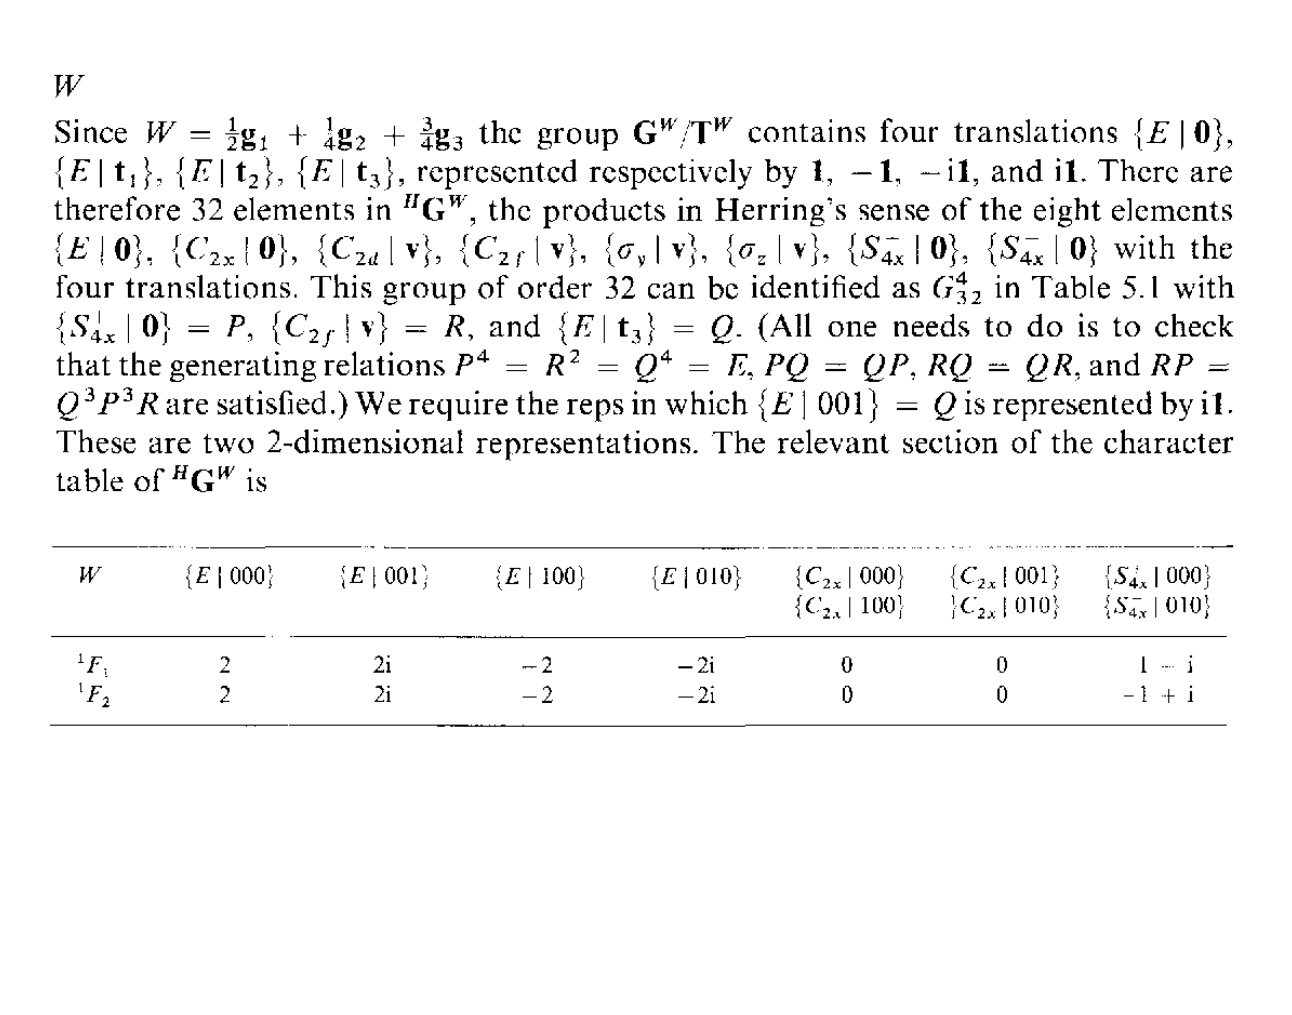
\includegraphics[width=0.92\textwidth]{c3_wchar_p1.png}
\end{figure}
\begin{figure}[H]
\centering
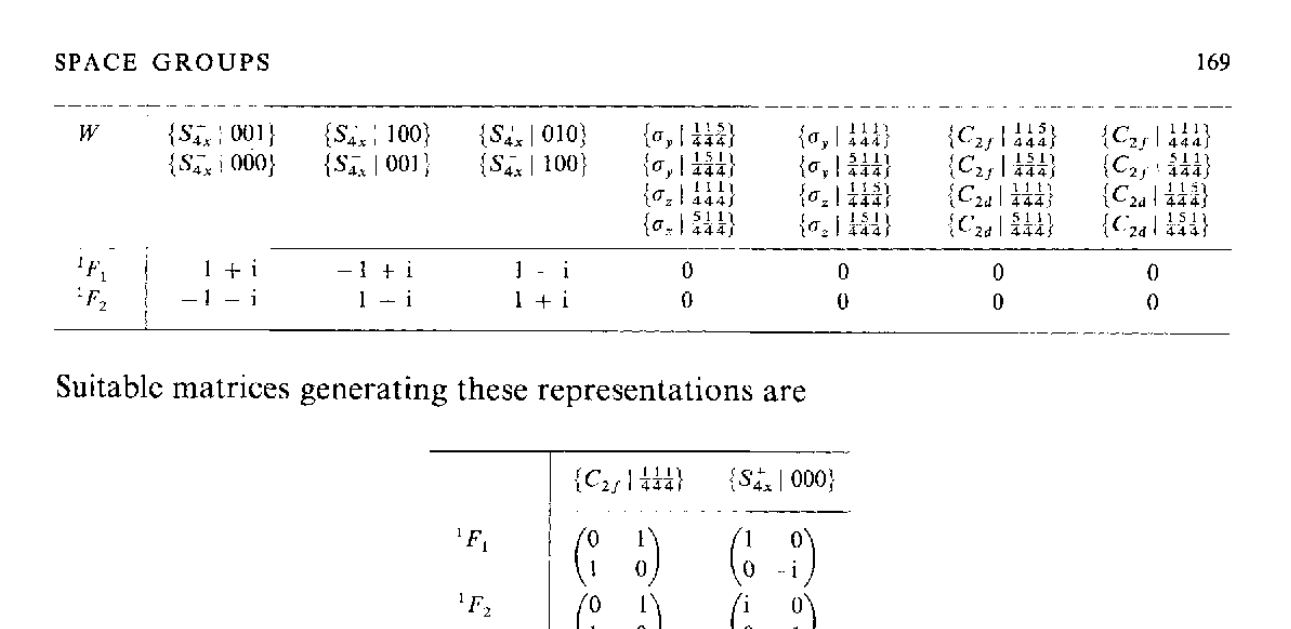
\includegraphics[width=0.92\textwidth]{c3_wchar_p2.png}
\caption*{\textbf{W 点}\ ${}^{H}\mathbf{G}^{W}$ 的特征标表（原书扫描占位，跨第 168--169 页）。}
\end{figure}

生成这些表示的合适矩阵是
\begin{center}
\begin{tabular}{lcc}
 & $\{C_{2f} \mid {\frac{1}{4}}{\frac{1}{4}}{\frac{1}{4}}\}$ & $\{S^{+}_{4x} \mid 000\}$\\[0.5ex]
${}^{1}\Gamma_{1}$ & $\begin{pmatrix} 0 & 1\\ 1 & 0 \end{pmatrix}$ & $\begin{pmatrix} 1 & 0\\ 0 & -i \end{pmatrix}$\\[2ex]
${}^{1}\Gamma_{2}$ & $\begin{pmatrix} 0 & 1\\ 1 & 0 \end{pmatrix}$ & $\begin{pmatrix} i & 0\\ 0 & -1 \end{pmatrix}$
\end{tabular}
\end{center}

\subsection*{X}

由于 $X = (\frac{1}{2}0\frac{1}{2})$，群 ${}^{H}\mathbf{G}^{X}$ 含有两个平移 $\{E \mid \mathbf{0}\}$ 与 $\{E \mid \mathbf{t}_{1}\}$，分别由 $\mathbf{1}$ 与 $-\mathbf{1}$ 表示。于是 ${}^{H}\mathbf{G}^{X}$ 中有 32 个元素，即 16 个元素 $\{E \mid \mathbf{0}\}$、$\{C_{2y} \mid \mathbf{0}\}$、$\{C^{+}_{4y} \mid \mathbf{v}\}$、$\{C_{2x} \mid \mathbf{0}\}$、$\{C_{2z} \mid \mathbf{0}\}$、$\{C_{2c} \mid \mathbf{v}\}$、$\{C_{2e} \mid \mathbf{v}\}$、$\{I \mid \mathbf{v}\}$、$\{\sigma_{y} \mid \mathbf{v}\}$、$\{S^{+}_{4y} \mid \mathbf{0}\}$、$\{\sigma_{x} \mid \mathbf{v}\}$、$\{\sigma_{z} \mid \mathbf{v}\}$、$\{\sigma_{dc} \mid \mathbf{0}\}$ 与 $\{\sigma_{de} \mid \mathbf{0}\}$ 与这两个平移在 Herring 意义下的乘积。这个 32 阶的群可以辨认为表 5.1 中的 $G^{2}_{32}$，取 $\{\sigma_{x} \mid \mathbf{v}\} = P$、$\{S^{+}_{4y} \mid \mathbf{0}\} = Q$、$\{C_{2x} \mid \mathbf{0}\} = R$。我们需要的是 $\{E \mid \mathbf{t}_{1}\} = P^{2}$ 由 $-\mathbf{1}$ 表示的那些表示。这是四个二维表示。${}^{H}\mathbf{G}^{X}$ 的特征标表的有关部分为

\begin{figure}[H]
\centering
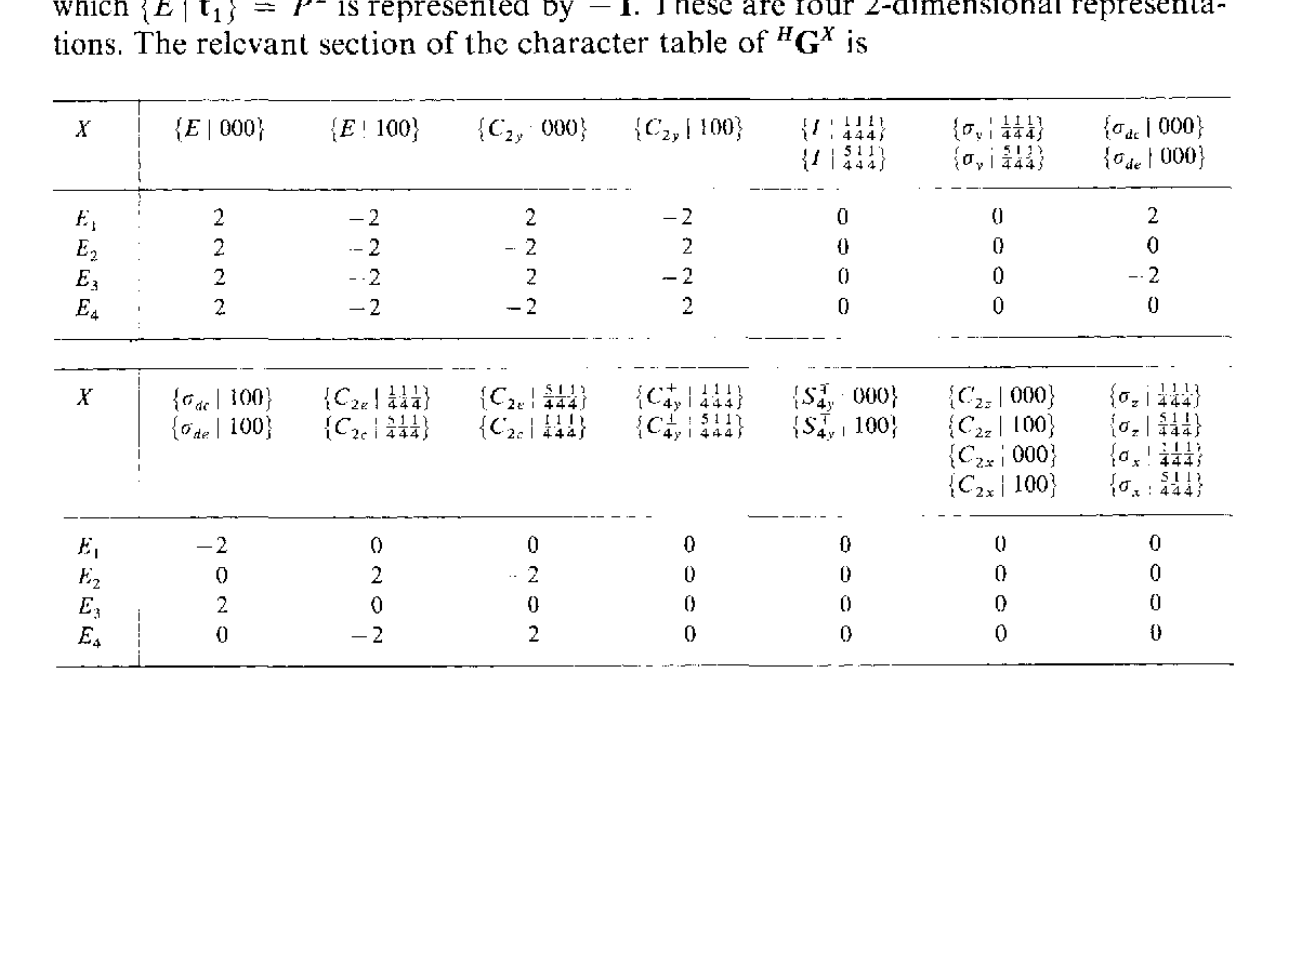
\includegraphics[width=0.92\textwidth]{c3_xchar.png}
\caption*{\textbf{X 点}\ ${}^{H}\mathbf{G}^{X}$ 的特征标表（原书扫描占位）。}
\end{figure}

生成这些表示的合适矩阵是
\begin{center}
\begin{tabular}{lccc}
 & $\{\sigma_{x} \mid {\frac{1}{4}}{\frac{1}{4}}{\frac{1}{4}}\}$ & $\{S^{+}_{4y} \mid 000\}$ & $\{C_{2x} \mid 000\}$\\[0.5ex]
$E_{1}$ & $\begin{pmatrix} 0 & -1\\ 1 & 0 \end{pmatrix}$ & $\begin{pmatrix} 0 & 1\\ 1 & 0 \end{pmatrix}$ & $\begin{pmatrix} 0 & 1\\ 1 & 0 \end{pmatrix}$\\[2ex]
$E_{2}$ & $\begin{pmatrix} 0 & -1\\ 1 & 0 \end{pmatrix}$ & $\begin{pmatrix} 0 & 1\\ -1 & 0 \end{pmatrix}$ & $\begin{pmatrix} 0 & 1\\ 1 & 0 \end{pmatrix}$\\[2ex]
$E_{3}$ & $\begin{pmatrix} 0 & -1\\ 1 & 0 \end{pmatrix}$ & $\begin{pmatrix} 0 & -1\\ -1 & 0 \end{pmatrix}$ & $\begin{pmatrix} 0 & 1\\ 1 & 0 \end{pmatrix}$\\[2ex]
$E_{4}$ & $\begin{pmatrix} 0 & -1\\ 1 & 0 \end{pmatrix}$ & $\begin{pmatrix} 0 & -1\\ 1 & 0 \end{pmatrix}$ & $\begin{pmatrix} 0 & 1\\ 1 & 0 \end{pmatrix}$
\end{tabular}
\end{center}

\subsection*{L}

由于 $L = (\frac{1}{2}\frac{1}{2}\frac{1}{2})$，群 ${}^{H}\mathbf{G}^{L}$ 含有两个平移 $\{E \mid \mathbf{0}\}$ 与 $\{E \mid \mathbf{t}_{1}\}$，分别由 $\mathbf{1}$ 与 $-\mathbf{1}$ 表示。该群阶为 24，同构于 $3m\ (C_{3v}) \otimes \mathbf{J} \otimes \mathbf{T}_{1}$，其中 $3m\ (C_{3v})$ 含有六个元素 $\{E \mid \mathbf{0}\}$、$\{C^{\pm}_{31} \mid \mathbf{0}\}$、$\{\sigma_{db} \mid \mathbf{0}\}$、$\{\sigma_{dc} \mid \mathbf{0}\}$、$\{\sigma_{df} \mid \mathbf{0}\}$，$\mathbf{J}$ 含有 $\{E \mid \mathbf{0}\}$ 与 $\{I \mid \mathbf{v}\}$，$\mathbf{T}_{1}$ 含有两个平移 $\{E \mid \mathbf{0}\}$ 与 $\{E \mid \mathbf{t}_{1}\}$。因此有六个小表示，${}^{H}\mathbf{G}^{L}$ 的特征标表的有关部分由表 2.2 可见为
\begin{center}
\begin{tabular}{lcccccc}
$L$ & $\{E \mid 000\}$ & $\{C^{\pm}_{31} \mid 000\}$ & $\begin{array}{c}\{\sigma_{db} \mid 000\}\\ \{\sigma_{dc} \mid 000\}\\ \{\sigma_{df} \mid 000\}\end{array}$ & $\{I \mid {\frac{1}{4}}{\frac{1}{4}}{\frac{1}{4}}\}$ & $\{S^{\mp}_{61} \mid {\frac{1}{4}}{\frac{1}{4}}{\frac{1}{4}}\}$ & $\begin{array}{c}\{C_{2b} \mid {\frac{1}{4}}{\frac{1}{4}}{\frac{1}{4}}\}\\ \{C_{2e} \mid {\frac{1}{4}}{\frac{1}{4}}{\frac{1}{4}}\}\\ \{C_{2f} \mid {\frac{1}{4}}{\frac{1}{4}}{\frac{1}{4}}\}\end{array}$\\
$A_{1g}$ & $1$ & $1$ & $1$ & $1$ & $1$ & $1$\\
$A_{2g}$ & $1$ & $1$ & $-1$ & $1$ & $1$ & $-1$\\
$E_{g}$ & $2$ & $-1$ & $0$ & $2$ & $-1$ & $0$\\
$A_{1u}$ & $1$ & $1$ & $1$ & $-1$ & $-1$ & $-1$\\
$A_{2u}$ & $1$ & $1$ & $-1$ & $-1$ & $-1$ & $1$\\
$E_{u}$ & $2$ & $-1$ & $0$ & $-2$ & $1$ & $0$
\end{tabular}
\end{center}
二维表示的生成矩阵可由表 2.3 得到。可以看到，碰巧 $Fd3m$ 中属于 $Q$ 和 $L$ 的表示的形式与 $Fm3m$ 中的完全一样。我们给出的关于这种情况何时必然发生的规则因此是充分的但不必要的；从这个例子我们看到，即使 $\mathbf{k}_{1}$ 位于布里渊区面上且空间群是非点式的，$\mathbf{G}^{\mathbf{k}_{1}}$ 的小表示偶尔也与 $\overline{\mathbf{G}}^{\mathbf{k}_{1}}$ 的表示具有相同的形式。


\end{document}
